% Options for packages loaded elsewhere
\PassOptionsToPackage{unicode}{hyperref}
\PassOptionsToPackage{hyphens}{url}
%
\documentclass[
]{book}
\usepackage{lmodern}
\usepackage{amsmath}
\usepackage{ifxetex,ifluatex}
\ifnum 0\ifxetex 1\fi\ifluatex 1\fi=0 % if pdftex
  \usepackage[T1]{fontenc}
  \usepackage[utf8]{inputenc}
  \usepackage{textcomp} % provide euro and other symbols
  \usepackage{amssymb}
\else % if luatex or xetex
  \usepackage{unicode-math}
  \defaultfontfeatures{Scale=MatchLowercase}
  \defaultfontfeatures[\rmfamily]{Ligatures=TeX,Scale=1}
\fi
% Use upquote if available, for straight quotes in verbatim environments
\IfFileExists{upquote.sty}{\usepackage{upquote}}{}
\IfFileExists{microtype.sty}{% use microtype if available
  \usepackage[]{microtype}
  \UseMicrotypeSet[protrusion]{basicmath} % disable protrusion for tt fonts
}{}
\makeatletter
\@ifundefined{KOMAClassName}{% if non-KOMA class
  \IfFileExists{parskip.sty}{%
    \usepackage{parskip}
  }{% else
    \setlength{\parindent}{0pt}
    \setlength{\parskip}{6pt plus 2pt minus 1pt}}
}{% if KOMA class
  \KOMAoptions{parskip=half}}
\makeatother
\usepackage{xcolor}
\IfFileExists{xurl.sty}{\usepackage{xurl}}{} % add URL line breaks if available
\IfFileExists{bookmark.sty}{\usepackage{bookmark}}{\usepackage{hyperref}}
\hypersetup{
  pdftitle={회귀모형 R 실습},
  pdfauthor={서울시립대학교 통계학과 이용희},
  hidelinks,
  pdfcreator={LaTeX via pandoc}}
\urlstyle{same} % disable monospaced font for URLs
\usepackage{color}
\usepackage{fancyvrb}
\newcommand{\VerbBar}{|}
\newcommand{\VERB}{\Verb[commandchars=\\\{\}]}
\DefineVerbatimEnvironment{Highlighting}{Verbatim}{commandchars=\\\{\}}
% Add ',fontsize=\small' for more characters per line
\usepackage{framed}
\definecolor{shadecolor}{RGB}{248,248,248}
\newenvironment{Shaded}{\begin{snugshade}}{\end{snugshade}}
\newcommand{\AlertTok}[1]{\textcolor[rgb]{0.94,0.16,0.16}{#1}}
\newcommand{\AnnotationTok}[1]{\textcolor[rgb]{0.56,0.35,0.01}{\textbf{\textit{#1}}}}
\newcommand{\AttributeTok}[1]{\textcolor[rgb]{0.77,0.63,0.00}{#1}}
\newcommand{\BaseNTok}[1]{\textcolor[rgb]{0.00,0.00,0.81}{#1}}
\newcommand{\BuiltInTok}[1]{#1}
\newcommand{\CharTok}[1]{\textcolor[rgb]{0.31,0.60,0.02}{#1}}
\newcommand{\CommentTok}[1]{\textcolor[rgb]{0.56,0.35,0.01}{\textit{#1}}}
\newcommand{\CommentVarTok}[1]{\textcolor[rgb]{0.56,0.35,0.01}{\textbf{\textit{#1}}}}
\newcommand{\ConstantTok}[1]{\textcolor[rgb]{0.00,0.00,0.00}{#1}}
\newcommand{\ControlFlowTok}[1]{\textcolor[rgb]{0.13,0.29,0.53}{\textbf{#1}}}
\newcommand{\DataTypeTok}[1]{\textcolor[rgb]{0.13,0.29,0.53}{#1}}
\newcommand{\DecValTok}[1]{\textcolor[rgb]{0.00,0.00,0.81}{#1}}
\newcommand{\DocumentationTok}[1]{\textcolor[rgb]{0.56,0.35,0.01}{\textbf{\textit{#1}}}}
\newcommand{\ErrorTok}[1]{\textcolor[rgb]{0.64,0.00,0.00}{\textbf{#1}}}
\newcommand{\ExtensionTok}[1]{#1}
\newcommand{\FloatTok}[1]{\textcolor[rgb]{0.00,0.00,0.81}{#1}}
\newcommand{\FunctionTok}[1]{\textcolor[rgb]{0.00,0.00,0.00}{#1}}
\newcommand{\ImportTok}[1]{#1}
\newcommand{\InformationTok}[1]{\textcolor[rgb]{0.56,0.35,0.01}{\textbf{\textit{#1}}}}
\newcommand{\KeywordTok}[1]{\textcolor[rgb]{0.13,0.29,0.53}{\textbf{#1}}}
\newcommand{\NormalTok}[1]{#1}
\newcommand{\OperatorTok}[1]{\textcolor[rgb]{0.81,0.36,0.00}{\textbf{#1}}}
\newcommand{\OtherTok}[1]{\textcolor[rgb]{0.56,0.35,0.01}{#1}}
\newcommand{\PreprocessorTok}[1]{\textcolor[rgb]{0.56,0.35,0.01}{\textit{#1}}}
\newcommand{\RegionMarkerTok}[1]{#1}
\newcommand{\SpecialCharTok}[1]{\textcolor[rgb]{0.00,0.00,0.00}{#1}}
\newcommand{\SpecialStringTok}[1]{\textcolor[rgb]{0.31,0.60,0.02}{#1}}
\newcommand{\StringTok}[1]{\textcolor[rgb]{0.31,0.60,0.02}{#1}}
\newcommand{\VariableTok}[1]{\textcolor[rgb]{0.00,0.00,0.00}{#1}}
\newcommand{\VerbatimStringTok}[1]{\textcolor[rgb]{0.31,0.60,0.02}{#1}}
\newcommand{\WarningTok}[1]{\textcolor[rgb]{0.56,0.35,0.01}{\textbf{\textit{#1}}}}
\usepackage{longtable,booktabs}
\usepackage{calc} % for calculating minipage widths
% Correct order of tables after \paragraph or \subparagraph
\usepackage{etoolbox}
\makeatletter
\patchcmd\longtable{\par}{\if@noskipsec\mbox{}\fi\par}{}{}
\makeatother
% Allow footnotes in longtable head/foot
\IfFileExists{footnotehyper.sty}{\usepackage{footnotehyper}}{\usepackage{footnote}}
\makesavenoteenv{longtable}
\usepackage{graphicx}
\makeatletter
\def\maxwidth{\ifdim\Gin@nat@width>\linewidth\linewidth\else\Gin@nat@width\fi}
\def\maxheight{\ifdim\Gin@nat@height>\textheight\textheight\else\Gin@nat@height\fi}
\makeatother
% Scale images if necessary, so that they will not overflow the page
% margins by default, and it is still possible to overwrite the defaults
% using explicit options in \includegraphics[width, height, ...]{}
\setkeys{Gin}{width=\maxwidth,height=\maxheight,keepaspectratio}
% Set default figure placement to htbp
\makeatletter
\def\fps@figure{htbp}
\makeatother
\setlength{\emergencystretch}{3em} % prevent overfull lines
\providecommand{\tightlist}{%
  \setlength{\itemsep}{0pt}\setlength{\parskip}{0pt}}
\setcounter{secnumdepth}{5}
%----- my options----------------
\usepackage[hangul]{kotex}
\usepackage{bm}
\usepackage{fullpage}

\newcommand{\pardiff}[2]{\frac{\partial #1}{\partial #2 }}
\newcommand{\pardiffl}[2]{{\partial #1}/{\partial #2 }}
\newcommand{\pardiffd}[2]{\frac{\partial^2 #1}{\partial #2^t \partial #2 }}
\newcommand{\pardiffdd}[3]{\frac{\partial^2 #1}{\partial #2 \partial #3 }}
\newcommand{\norm}[1]{\left\lVert#1\right\rVert}
\newcommand{\hatmat}{\bm X ({\bm X}^t {\bm X} )^{-1} {\bm X}^t}
\newcommand{\hatmatt}[1]{\bm X_{#1} ({\bm X}_{#1}^t {\bm X}_{#1})^{-1} {\bm X}_{#1}^t}

%--------- from bookdown.org --------------

\usepackage{booktabs}


\usepackage{framed,color}
\definecolor{shadecolor}{RGB}{248,248,248}

\renewcommand{\textfraction}{0.05}
\renewcommand{\topfraction}{0.8}
\renewcommand{\bottomfraction}{0.8}
\renewcommand{\floatpagefraction}{0.75}

\renewenvironment{quote}{\begin{VF}}{\end{VF}}
\let\oldhref\href
\renewcommand{\href}[2]{#2\footnote{\url{#1}}}

\makeatletter
\newenvironment{kframe}{%
\medskip{}
\setlength{\fboxsep}{.8em}
 \def\at@end@of@kframe{}%
 \ifinner\ifhmode%
  \def\at@end@of@kframe{\end{minipage}}%
  \begin{minipage}{\columnwidth}%
 \fi\fi%
 \def\FrameCommand##1{\hskip\@totalleftmargin \hskip-\fboxsep
 \colorbox{shadecolor}{##1}\hskip-\fboxsep
     % There is no \\@totalrightmargin, so:
     \hskip-\linewidth \hskip-\@totalleftmargin \hskip\columnwidth}%
 \MakeFramed {\advance\hsize-\width
   \@totalleftmargin\z@ \linewidth\hsize
   \@setminipage}}%
 {\par\unskip\endMakeFramed%
 \at@end@of@kframe}
\makeatother

\makeatletter

\@ifundefined{Shaded}{
}{\renewenvironment{Shaded}{\begin{kframe}}{\end{kframe}}}
\makeatother

\newenvironment{rmdblock}[1]
  {
  \begin{itemize}
  \renewcommand{\labelitemi}{
    \raisebox{-.7\height}[0pt][0pt]{
      {\setkeys{Gin}{width=3em,keepaspectratio}\includegraphics{images/#1}}
    }
  }
  \setlength{\fboxsep}{1em}
  \begin{kframe}
  \item
  }
  {
  \end{kframe}
  \end{itemize}
  }
  
\newenvironment{rmdnote}
  {\begin{rmdblock}{note}}
  {\end{rmdblock}}
  
\newenvironment{rmdcaution}
  {\begin{rmdblock}{caution}}
  {\end{rmdblock}}
  
\newenvironment{rmdimportant}
  {\begin{rmdblock}{important}}
  {\end{rmdblock}}
  
\newenvironment{rmdtip}
  {\begin{rmdblock}{tip}}
  {\end{rmdblock}}
  
\newenvironment{rmdwarning}
  {\begin{rmdblock}{warning}}
  {\end{rmdblock}}
  


\usepackage{makeidx}
\makeindex

\urlstyle{tt}

\usepackage{amsthm}
\makeatletter
 \def\thm@space@setup{%
   \thm@preskip=8pt plus 2pt minus 4pt
   \thm@postskip=\thm@preskip
}
\makeatother

\frontmatter
\usepackage{booktabs}
\usepackage{longtable}
\usepackage{array}
\usepackage{multirow}
\usepackage{wrapfig}
\usepackage{float}
\usepackage{colortbl}
\usepackage{pdflscape}
\usepackage{tabu}
\usepackage{threeparttable}
\usepackage{threeparttablex}
\usepackage[normalem]{ulem}
\usepackage{makecell}
\usepackage{xcolor}
\ifluatex
  \usepackage{selnolig}  % disable illegal ligatures
\fi
\usepackage[]{natbib}
\bibliographystyle{apalike}

\title{회귀모형 R 실습}
\author{서울시립대학교 통계학과 이용희}
\date{2021-05-25}

\begin{document}
\maketitle

{
\setcounter{tocdepth}{1}
\tableofcontents
}
\hypertarget{preface}{%
\chapter*{Preface}\label{preface}}


이 책은 일반 선형모형에 대한 R 프로그램과 결과에 대하여 설명합니다.

다음과 같은 R 패키지가 필요합니다.

\begin{verbatim}
library(ggplot2)
library(dplyr)
library(tidyr)
library(kableExtra)
library(regbook)
library(ellipse)
library(car)
library(MASS)
library(Matrix)
library(agricolae)
library(emmeans)
library(car)
library(leaps)
library(olsrr)
\end{verbatim}

\begin{rmdimportant}
이 책에서 사용된 기호, 표기법, 프로그램의 규칙과 쓰임은 다음과 같습니다.

\begin{itemize}
\tightlist
\item
  스칼라(scalar)와 일변량 확률변수는 일반적으로 보통 글씨체의 소문자로 표기한다. 특별한 이유가 있는 경우 대문자로 표시할 것이다.
\item
  벡터, 행렬, 다변량 확률벡터는 굵은 글씨체로 표기한다.
\item
  통계 프로그램은 \texttt{R}을 이용하였다. 각 예제에 사용된 \texttt{R} 프로그램은 코드 상자를 열면 나타난다.
\item
  통계 프로그램은 \texttt{R}에 대한 기초는 저자의 홈페이지에 있는 \href{https://ilovedata.github.io/computing/}{안내 사이트}에서 먼저 학습할 것을 권장한다.
\end{itemize}
\end{rmdimportant}

\hypertarget{chap02}{%
\chapter{단순회귀 예제}\label{chap02}}

\hypertarget{mammal-uxc790uxb8cc}{%
\section{MAMMAL 자료}\label{mammal-uxc790uxb8cc}}

이제 교재 109 페이지(연습문제 2.25) 에서 소개된 포유류의 뇌의 무게와 몸무게에 대한 자료 데이터프레임 \texttt{Mammal}를 사용할 수 있다.

\begin{Shaded}
\begin{Highlighting}[]
\FunctionTok{head}\NormalTok{(mammal)}
\end{Highlighting}
\end{Shaded}

\begin{verbatim}
##              brain    body
## Arctic fox  44.500   3.385
## Owl monkey  15.499   0.480
## Beaver       8.100   1.350
## Cow        423.012 464.983
## Gray wolf  119.498  36.328
## Goat       114.996  27.660
\end{verbatim}

\begin{Shaded}
\begin{Highlighting}[]
\FunctionTok{plot}\NormalTok{(brain}\SpecialCharTok{\textasciitilde{}}\NormalTok{body, }\AttributeTok{data=}\NormalTok{mammal) }
\end{Highlighting}
\end{Shaded}

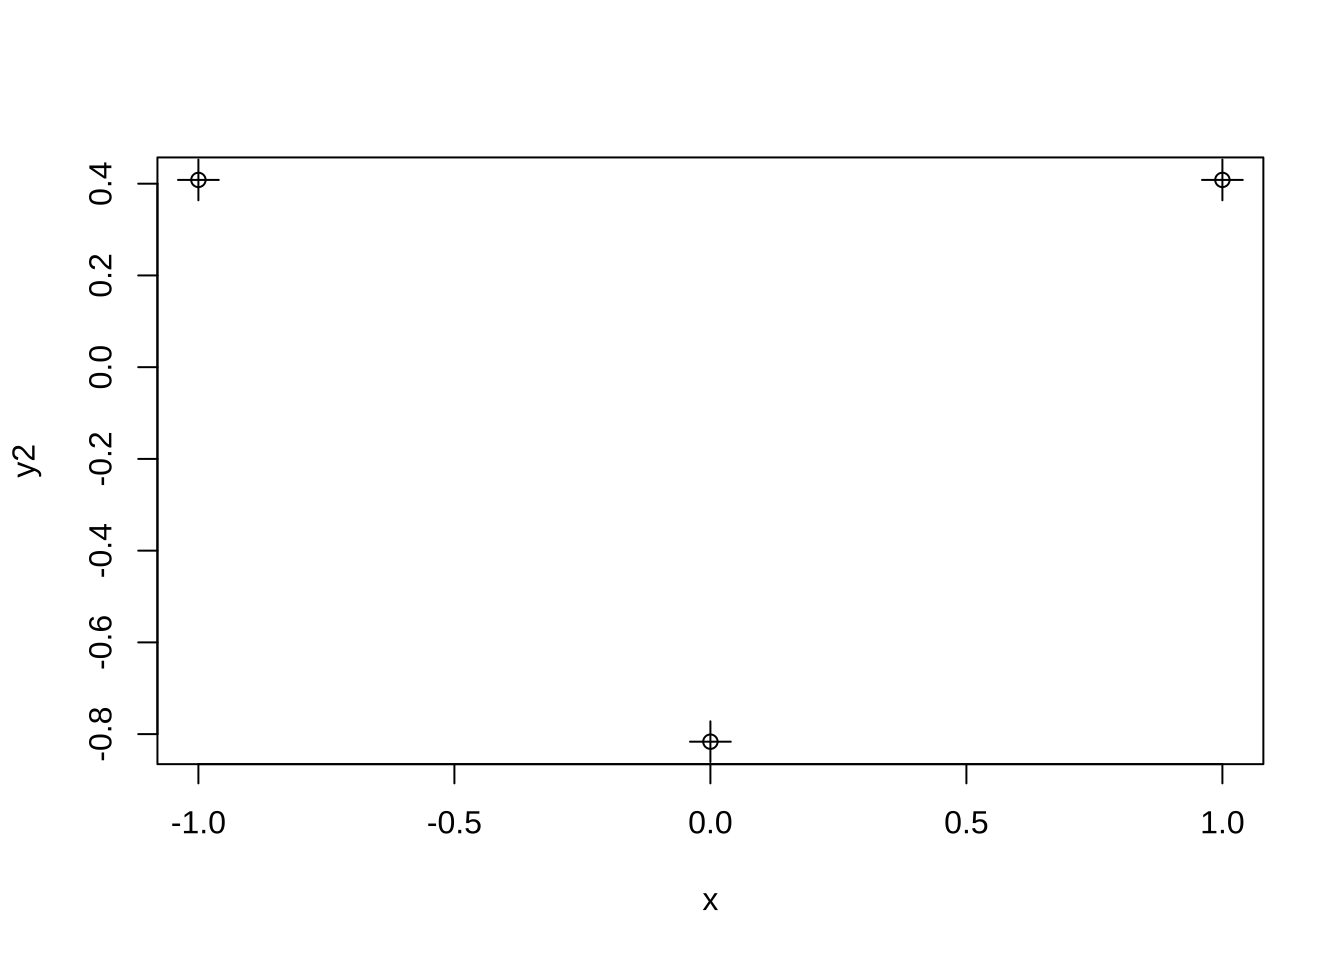
\includegraphics{lmpractice_files/figure-latex/unnamed-chunk-4-1.pdf}

\hypertarget{uxbcc0uxc218uxc758-uxbcc0uxd658}{%
\section{변수의 변환}\label{uxbcc0uxc218uxc758-uxbcc0uxd658}}

데이터프레임 \texttt{Mammal}의 두 두 변수를 \texttt{log10()} 함수를 이용하여 변환하고 새로운 변수를 만들자.

\begin{Shaded}
\begin{Highlighting}[]
\NormalTok{mammal}\SpecialCharTok{$}\NormalTok{lbrain }\OtherTok{\textless{}{-}} \FunctionTok{log10}\NormalTok{(mammal}\SpecialCharTok{$}\NormalTok{brain)}
\NormalTok{mammal}\SpecialCharTok{$}\NormalTok{lbody }\OtherTok{\textless{}{-}} \FunctionTok{log10}\NormalTok{(mammal}\SpecialCharTok{$}\NormalTok{body)}
\FunctionTok{head}\NormalTok{(mammal)}
\end{Highlighting}
\end{Shaded}

\begin{verbatim}
##              brain    body   lbrain      lbody
## Arctic fox  44.500   3.385 1.648360  0.5295587
## Owl monkey  15.499   0.480 1.190304 -0.3187588
## Beaver       8.100   1.350 0.908485  0.1303338
## Cow        423.012 464.983 2.626353  2.6674371
## Gray wolf  119.498  36.328 2.077361  1.5602415
## Goat       114.996  27.660 2.060683  1.4418522
\end{verbatim}

\begin{Shaded}
\begin{Highlighting}[]
\FunctionTok{plot}\NormalTok{(lbrain}\SpecialCharTok{\textasciitilde{}}\NormalTok{lbody, }\AttributeTok{data=}\NormalTok{mammal)}
\end{Highlighting}
\end{Shaded}

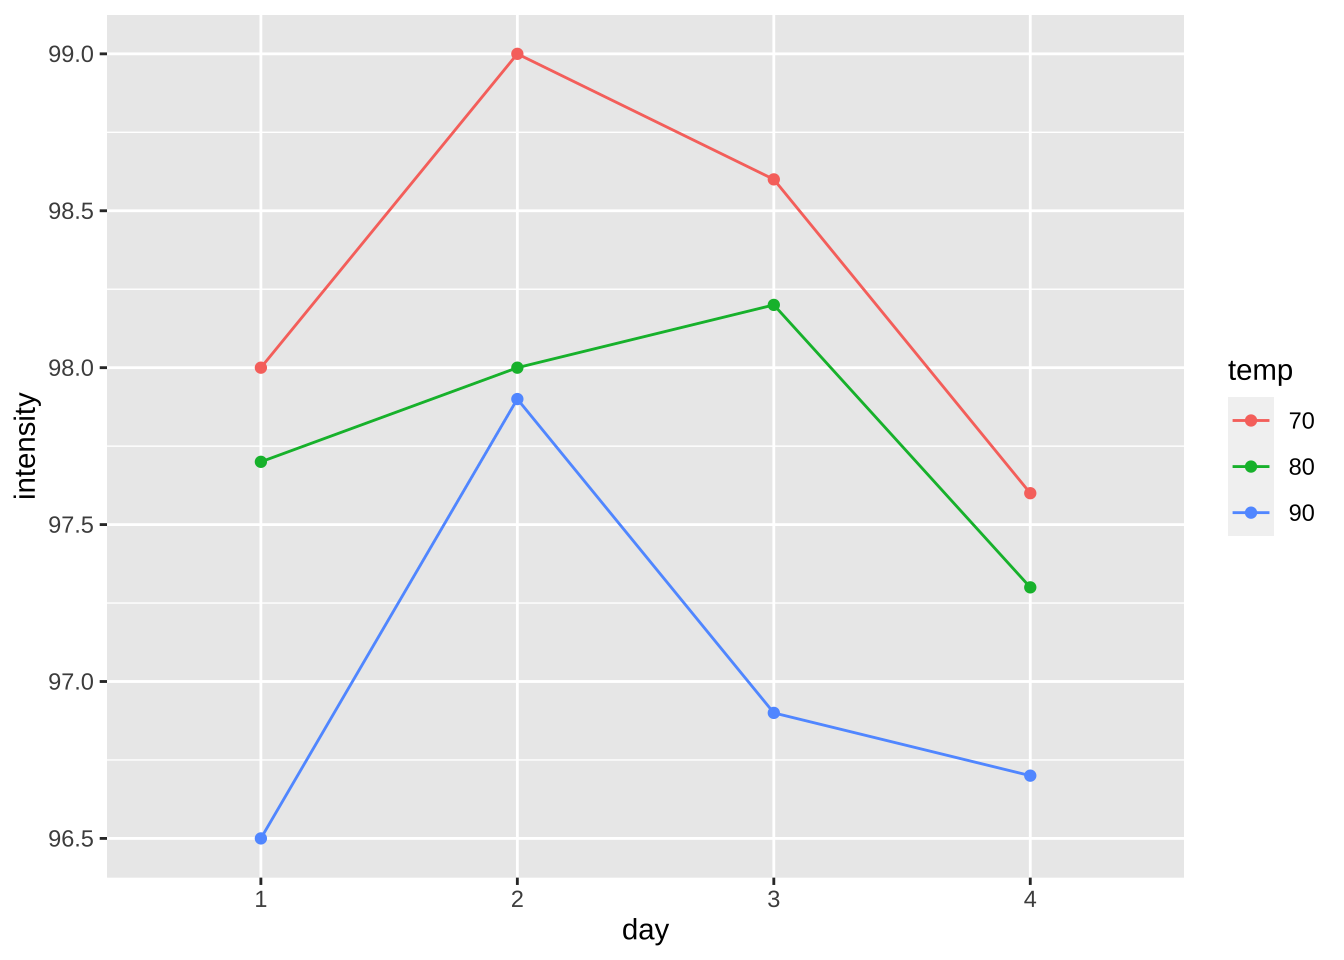
\includegraphics{lmpractice_files/figure-latex/unnamed-chunk-5-1.pdf}

\hypertarget{uxd2b9uxbcc4uxd55c-uxc790uxb8ccuxb97c-uxcc3euxae30}{%
\section{특별한 자료를 찾기}\label{uxd2b9uxbcc4uxd55c-uxc790uxb8ccuxb97c-uxcc3euxae30}}

자료에서 최대값과 최소값을 찾고 그 위치를 알아보는 방법은 여러 가지가 있다.

일단 산점도를 그린 후에 마우스를 이용하여 자료의 특성을 알아낼 수 있는 방법이 있다.
이러한 방법은 \texttt{plot()}으로 산범도를 그린 후에 \texttt{identify()}함수를 이용하면 마우스를 이용하여 동물의 이름을 볼수 있다.

\begin{Shaded}
\begin{Highlighting}[]
\FunctionTok{plot}\NormalTok{(lbrain}\SpecialCharTok{\textasciitilde{}}\NormalTok{lbody, }\AttributeTok{data=}\NormalTok{mammal)}
\FunctionTok{with}\NormalTok{(mammal, }\FunctionTok{identify}\NormalTok{(lbody, lbrain, }\AttributeTok{labels =} \FunctionTok{rownames}\NormalTok{(mammal)))}
\end{Highlighting}
\end{Shaded}

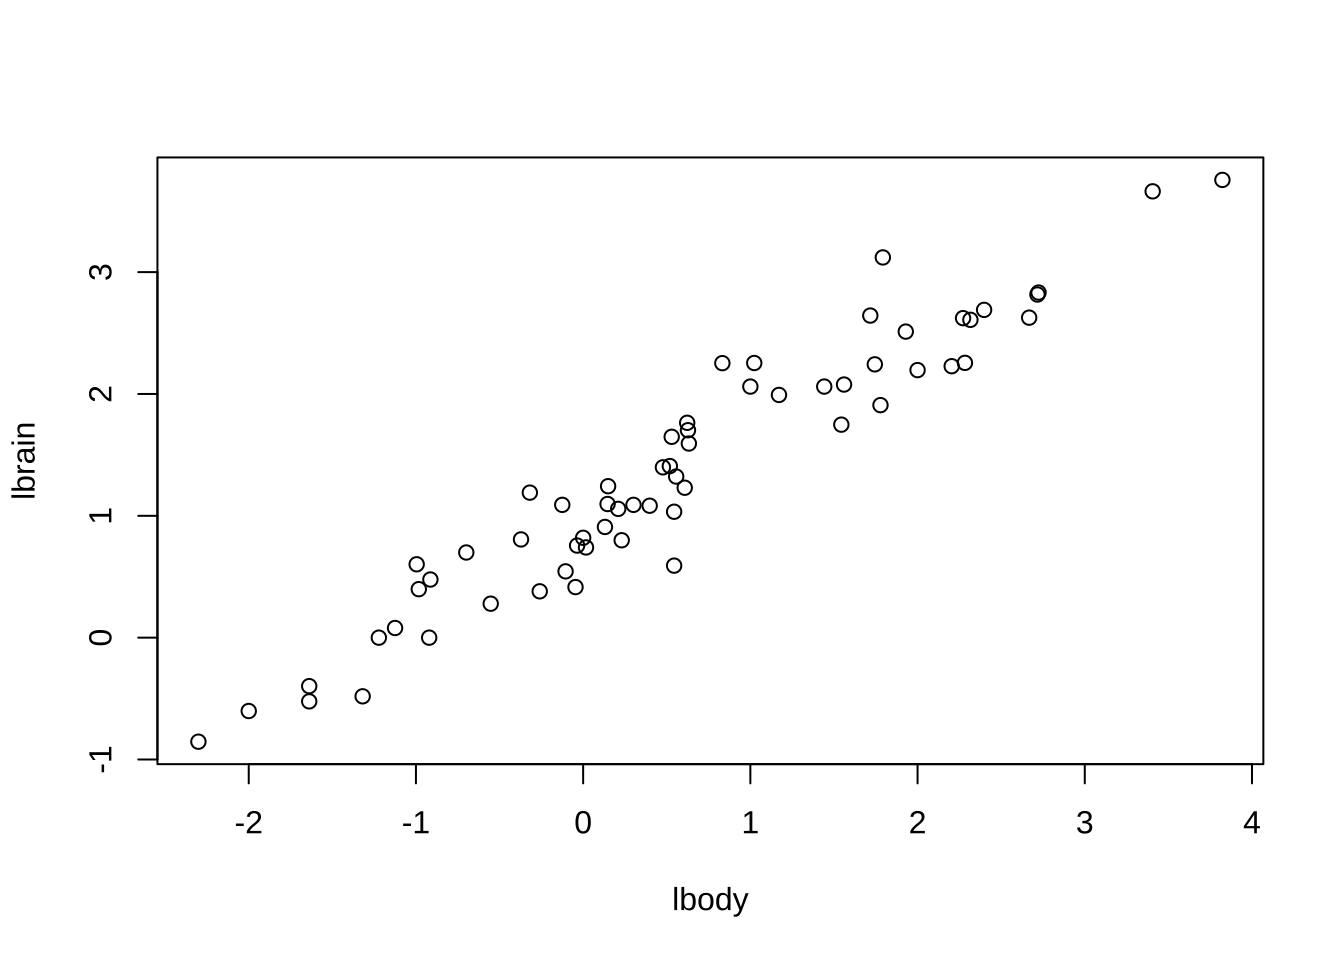
\includegraphics{lmpractice_files/figure-latex/unnamed-chunk-6-1.pdf}

\begin{verbatim}
## integer(0)
\end{verbatim}

데이터프레임 \texttt{mammal}에 있는 각 동물의 이름은 \texttt{rownames()} 함수를 통하여 알 수 있다.

\begin{Shaded}
\begin{Highlighting}[]
\FunctionTok{rownames}\NormalTok{(mammal)}
\end{Highlighting}
\end{Shaded}

\begin{verbatim}
##  [1] "Arctic fox"               "Owl monkey"               "Beaver"                   "Cow"                      "Gray wolf"                "Goat"                     "Roe deer"                 "Guinea pig"               "Vervet\""                 "Chinchilla"              
## [11] "Ground squirrel"          "Arctic ground squirrel"   "African giant pouched ra" "Lesser short-tailed shre" "Star-nosed mole"          "Nine-banded armadillo"    "Tree hyrax"               "N. American opossum"      "Asian elephant"           "Big brown bat"           
## [21] "Donkey"                   "Horse"                    "European hedgehog"        "Patas monkey"             "Cat"                      "Galago"                   "Genet"                    "Giraffe"                  "Gorilla"                  "Gray seal"               
## [31] "Rock hyrax1"              "Human"                    "African elephant"         "Water opossum"            "Rhesus monkey"            "Kangaroo"                 "Yellow-bellied marmot"    "Golden hamster"           "Mouse"                    "Little brown bat"        
## [41] "Slow loris"               "Okapi"                    "Rabbit"                   "Sheep"                    "Jaguar"                   "Chimpanzee"               "Baboon"                   "Desert hedgehog"          "Giant armadillo"          "Rock hyrax2"             
## [51] "Raccoon"                  "Rat"                      "E. American mole"         "Mole rat"                 "Musk shrew"               "Pig"                      "Echidna"                  "Brazilian tapir"          "Tenrec"                   "Phalanger"               
## [61] "Tree shrew"               "Red fox"
\end{verbatim}

\hypertarget{uxc790uxb8ccuxc758-uxc815uxb82c}{%
\section{자료의 정렬}\label{uxc790uxb8ccuxc758-uxc815uxb82c}}

\begin{itemize}
\item
  벡터에 있는 자료들을 크기순으로 정렬하고 싶다면 함수 \texttt{sort()}를 사용한다. 내림차순 정렬이 기본이고 내림차순으로 정렬하려면 \texttt{sort(x,\ decreasing\ =\ TRUE)}로 사용한다.
\item
  또한 벡터에 있는자료가 정렬된 순서(기본은 내림차순)를 구하고 싶으면 함수 \texttt{order()}를 사용한다. 내림차순의 순서를 구하고 싶으면 \texttt{order(x,\ decreasing\ =\ TRUE)}를 사용한다.
\end{itemize}

\begin{Shaded}
\begin{Highlighting}[]
\NormalTok{mammal}\SpecialCharTok{$}\NormalTok{body}
\end{Highlighting}
\end{Shaded}

\begin{verbatim}
##  [1]    3.385    0.480    1.350  464.983   36.328   27.660   14.831    1.040    4.190    0.425    0.101    0.920    1.000    0.005    0.060    3.500    2.000    1.700 2547.070    0.023  187.092  521.026    0.785   10.000    3.300    0.200    1.410  529.006  206.996   85.004    0.750   61.998
## [33] 6654.180    3.500    6.800   34.998    4.050    0.120    0.023    0.010    1.400  250.010    2.500   55.501  100.003   52.159   10.550    0.550   59.997    3.600    4.288    0.280    0.075    0.122    0.048  192.001    3.000  160.004    0.900    1.620    0.104    4.235
\end{verbatim}

\begin{Shaded}
\begin{Highlighting}[]
\FunctionTok{sort}\NormalTok{(mammal}\SpecialCharTok{$}\NormalTok{body)}
\end{Highlighting}
\end{Shaded}

\begin{verbatim}
##  [1]    0.005    0.010    0.023    0.023    0.048    0.060    0.075    0.101    0.104    0.120    0.122    0.200    0.280    0.425    0.480    0.550    0.750    0.785    0.900    0.920    1.000    1.040    1.350    1.400    1.410    1.620    1.700    2.000    2.500    3.000    3.300    3.385
## [33]    3.500    3.500    3.600    4.050    4.190    4.235    4.288    6.800   10.000   10.550   14.831   27.660   34.998   36.328   52.159   55.501   59.997   61.998   85.004  100.003  160.004  187.092  192.001  206.996  250.010  464.983  521.026  529.006 2547.070 6654.180
\end{verbatim}

\begin{Shaded}
\begin{Highlighting}[]
\FunctionTok{order}\NormalTok{(mammal}\SpecialCharTok{$}\NormalTok{body)}
\end{Highlighting}
\end{Shaded}

\begin{verbatim}
##  [1] 14 40 20 39 55 15 53 11 61 38 54 26 52 10  2 48 31 23 59 12 13  8  3 41 27 60 18 17 43 57 25  1 16 34 50 37  9 62 51 35 24 47  7  6 36  5 46 44 49 32 30 45 58 21 56 29 42  4 22 28 19 33
\end{verbatim}

자료의 최대값과 최소값을 구하는 함수는 \texttt{max()}와 \texttt{min()}이다.

\begin{Shaded}
\begin{Highlighting}[]
\FunctionTok{max}\NormalTok{(mammal}\SpecialCharTok{$}\NormalTok{lbrain)}
\end{Highlighting}
\end{Shaded}

\begin{verbatim}
## [1] 3.756778
\end{verbatim}

\begin{Shaded}
\begin{Highlighting}[]
\FunctionTok{min}\NormalTok{(mammal}\SpecialCharTok{$}\NormalTok{lbrain)}
\end{Highlighting}
\end{Shaded}

\begin{verbatim}
## [1] -0.853872
\end{verbatim}

자료의 최대값과 최소값의 순서을 구하는 함수는 \texttt{which.max()}와 \texttt{which.min()}이다.
이러한 함수를 통해서 구해진 순서의 자료에 대한 변수를 모두 볼 수 있다.

\begin{Shaded}
\begin{Highlighting}[]
\FunctionTok{which.max}\NormalTok{(mammal}\SpecialCharTok{$}\NormalTok{body)}
\end{Highlighting}
\end{Shaded}

\begin{verbatim}
## [1] 33
\end{verbatim}

\begin{Shaded}
\begin{Highlighting}[]
\NormalTok{mammal[}\FunctionTok{which.max}\NormalTok{(mammal}\SpecialCharTok{$}\NormalTok{body), ]}
\end{Highlighting}
\end{Shaded}

\begin{verbatim}
##                    brain    body   lbrain    lbody
## African elephant 5711.86 6654.18 3.756778 3.823095
\end{verbatim}

\begin{Shaded}
\begin{Highlighting}[]
\FunctionTok{which.min}\NormalTok{(mammal}\SpecialCharTok{$}\NormalTok{body)}
\end{Highlighting}
\end{Shaded}

\begin{verbatim}
## [1] 14
\end{verbatim}

\begin{Shaded}
\begin{Highlighting}[]
\NormalTok{mammal[}\FunctionTok{which.min}\NormalTok{(mammal}\SpecialCharTok{$}\NormalTok{body), ]}
\end{Highlighting}
\end{Shaded}

\begin{verbatim}
##                          brain  body    lbrain    lbody
## Lesser short-tailed shre  0.14 0.005 -0.853872 -2.30103
\end{verbatim}

\hypertarget{uxb2e8uxc21cuxd68cuxadc0uxbaa8uxd615uxc758-uxc801uxd569}{%
\section{단순회귀모형의 적합}\label{uxb2e8uxc21cuxd68cuxadc0uxbaa8uxd615uxc758-uxc801uxd569}}

다음과 같은 단순선형모형을 고려하자
\[ y_i = \beta_0 + \beta_1  x_i + \epsilon_i,~~ i=1,2,\dots,n \]

데이터프레임 \texttt{mammal}에서 로그변환된 몸무게 \texttt{lbody}을 독립변수 \(x\)로 하고 로그변환된 뇌무게를 \texttt{lbrain}을 종속변수 \(y\)로 하는 선형회귀직선의 절편과 기울기를 다음과 같이 함수 \texttt{lm()}을 이용하여 추정할 수 있다.

\begin{Shaded}
\begin{Highlighting}[]
\NormalTok{mammal.lm }\OtherTok{\textless{}{-}} \FunctionTok{lm}\NormalTok{(lbrain}\SpecialCharTok{\textasciitilde{}}\NormalTok{lbody, }\AttributeTok{data=}\NormalTok{mammal)}
\FunctionTok{summary}\NormalTok{(mammal.lm)}
\end{Highlighting}
\end{Shaded}

\begin{verbatim}
## 
## Call:
## lm(formula = lbrain ~ lbody, data = mammal)
## 
## Residuals:
##      Min       1Q   Median       3Q      Max 
## -0.74503 -0.21380 -0.02676  0.18934  0.84615 
## 
## Coefficients:
##             Estimate Std. Error t value Pr(>|t|)    
## (Intercept)  0.92713    0.04171   22.23   <2e-16 ***
## lbody        0.75169    0.02846   26.41   <2e-16 ***
## ---
## Signif. codes:  0 '***' 0.001 '**' 0.01 '*' 0.05 '.' 0.1 ' ' 1
## 
## Residual standard error: 0.3015 on 60 degrees of freedom
## Multiple R-squared:  0.9208, Adjusted R-squared:  0.9195 
## F-statistic: 697.4 on 1 and 60 DF,  p-value: < 2.2e-16
\end{verbatim}

\hypertarget{uxc0b0uxc810uxb3c4uxc5d0uxc11c-uxd2b9uxc815-uxc790uxb8ccuxc758-uxd45cuxc2dc}{%
\section{산점도에서 특정 자료의 표시}\label{uxc0b0uxc810uxb3c4uxc5d0uxc11c-uxd2b9uxc815-uxc790uxb8ccuxc758-uxd45cuxc2dc}}

산점도에 인간 \texttt{human} 자료 \((x_i, y_i)\)를 표시하고 싶으면 다음과 같은 \texttt{R} 코드를 사용할 수 있다. 산점도에 문자를 표시하는 함수 \texttt{text()}를 사용한다.

\begin{verbatim}
text(x,y, labels="A", cex=1.0, pos=1 )
\end{verbatim}

먼저 사람(\texttt{Human})에 대한 자료만 선택한다.

\begin{Shaded}
\begin{Highlighting}[]
\NormalTok{pickhuman }\OtherTok{\textless{}{-}} \FunctionTok{rownames}\NormalTok{(mammal) }\SpecialCharTok{==} \StringTok{"Human"}  
\NormalTok{pickhuman}
\end{Highlighting}
\end{Shaded}

\begin{verbatim}
##  [1] FALSE FALSE FALSE FALSE FALSE FALSE FALSE FALSE FALSE FALSE FALSE FALSE FALSE FALSE FALSE FALSE FALSE FALSE FALSE FALSE FALSE FALSE FALSE FALSE FALSE FALSE FALSE FALSE FALSE FALSE FALSE  TRUE FALSE FALSE FALSE FALSE FALSE FALSE FALSE FALSE FALSE FALSE FALSE FALSE FALSE FALSE FALSE FALSE FALSE
## [50] FALSE FALSE FALSE FALSE FALSE FALSE FALSE FALSE FALSE FALSE FALSE FALSE FALSE
\end{verbatim}

\begin{Shaded}
\begin{Highlighting}[]
\NormalTok{dat1 }\OtherTok{\textless{}{-}}\NormalTok{ mammal[pickhuman,]}
\NormalTok{dat1}
\end{Highlighting}
\end{Shaded}

\begin{verbatim}
##         brain   body   lbrain    lbody
## Human 1320.02 61.998 3.120581 1.792378
\end{verbatim}

함수 \texttt{points()} 는 지정된 좌표\((x,y)\)에 기호를 표시하며 기호의 종류는 \texttt{pch=}를 이용하여 숫자로 기호의 종류를 지정한다. 예를 들어 \texttt{pch=3}는 \texttt{+} 를 나타낸다.

함수\texttt{text()}에서 지정된 좌표\((x,y)\)에 문자로 표시를 하며 \texttt{labels=}는 산점도에 표시할 문자열을 지정하고 \texttt{cex=}은 문자의 크기, \texttt{pos=}은 표시할 위치를 지정한다.

\begin{Shaded}
\begin{Highlighting}[]
\FunctionTok{plot}\NormalTok{(lbrain}\SpecialCharTok{\textasciitilde{}}\NormalTok{lbody, }\AttributeTok{data=}\NormalTok{mammal)}
\FunctionTok{with}\NormalTok{(dat1, }\FunctionTok{points}\NormalTok{(lbody,lbrain, }\AttributeTok{pch=}\DecValTok{3}\NormalTok{))}
\FunctionTok{with}\NormalTok{(dat1, }\FunctionTok{text}\NormalTok{(lbody,lbrain, }\AttributeTok{labels =}\FunctionTok{rownames}\NormalTok{(dat1), }\AttributeTok{cex=}\FloatTok{1.2}\NormalTok{, }\AttributeTok{pos =} \DecValTok{4}\NormalTok{))}
\end{Highlighting}
\end{Shaded}

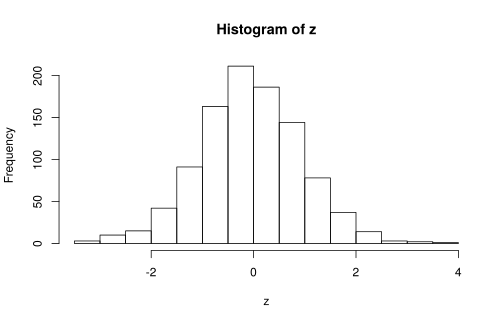
\includegraphics{lmpractice_files/figure-latex/unnamed-chunk-13-1.pdf}

위의 코드를 이용하면 다음과 같이 모든 자료의 이름을 표시할 수 있지만 읽기 힘든 그림이다.

\begin{Shaded}
\begin{Highlighting}[]
\FunctionTok{plot}\NormalTok{(lbrain}\SpecialCharTok{\textasciitilde{}}\NormalTok{lbody, }\AttributeTok{data=}\NormalTok{mammal)}
\FunctionTok{with}\NormalTok{(mammal, }\FunctionTok{text}\NormalTok{(lbody,lbrain, }\AttributeTok{labels =}\FunctionTok{rownames}\NormalTok{(mammal), }\AttributeTok{cex=}\FloatTok{0.6}\NormalTok{, }\AttributeTok{pos =} \DecValTok{1}\NormalTok{))}
\end{Highlighting}
\end{Shaded}

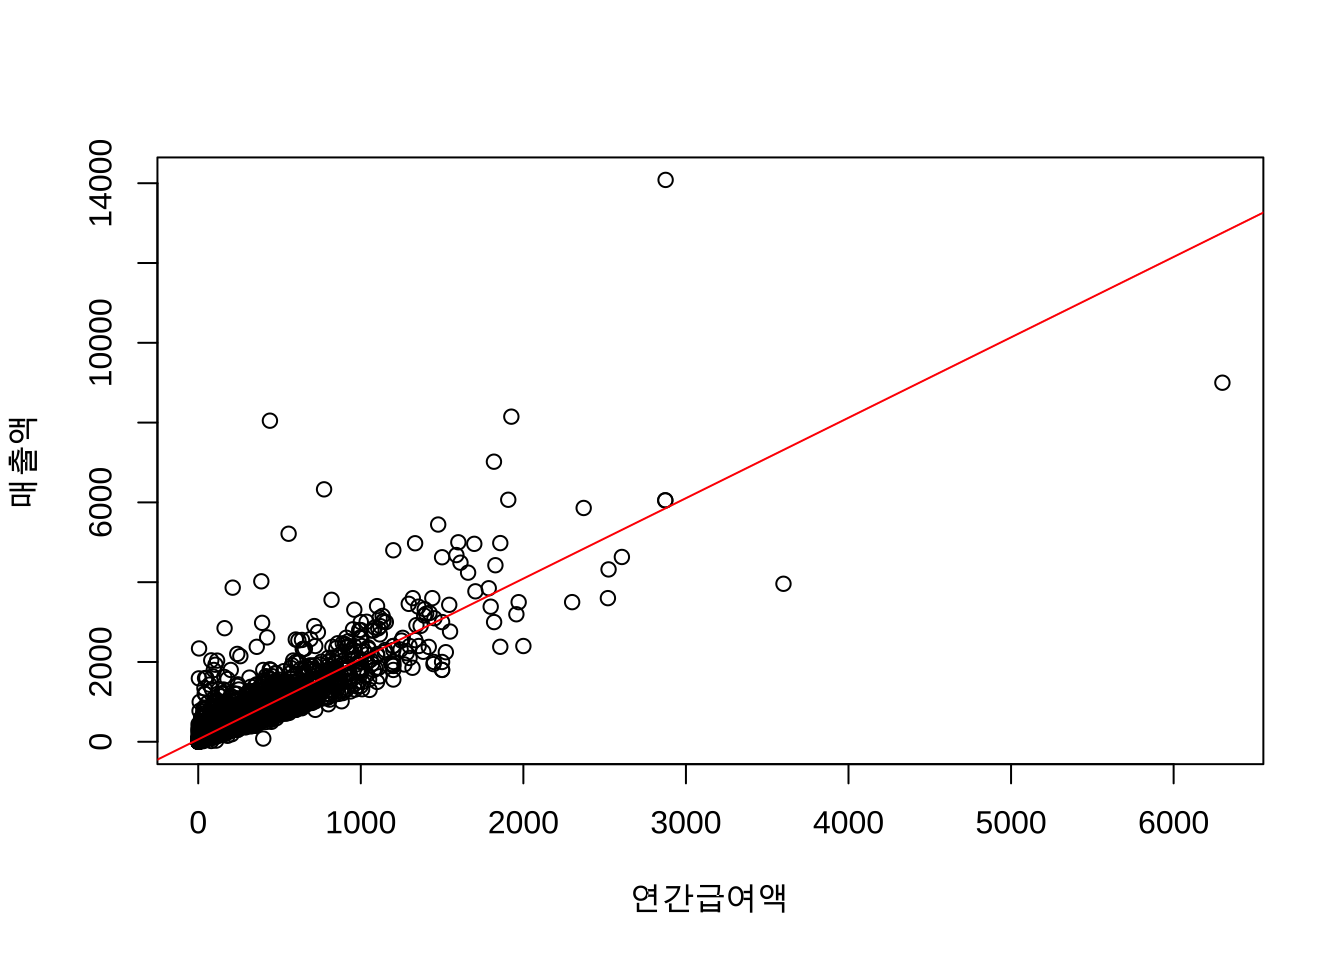
\includegraphics{lmpractice_files/figure-latex/unnamed-chunk-14-1.pdf}

\mainmatter

\hypertarget{chapter03}{%
\chapter{중회귀분석}\label{chapter03}}

예제 3.3에 나온 중고차 가격자료를 이용한 R 실습입니다.
\#\#

\hypertarget{uxc911uxace0uxcc28-uxc790uxb8cc}{%
\section{중고차 자료}\label{uxc911uxace0uxcc28-uxc790uxb8cc}}

\begin{Shaded}
\begin{Highlighting}[]
\FunctionTok{head}\NormalTok{(usedcars)}
\end{Highlighting}
\end{Shaded}

\begin{verbatim}
##   price year mileage   cc automatic
## 1   790   78  133462 1998         1
## 2  1380   39   33000 2000         1
## 3   270  109  120000 1800         0
## 4  1190   20   69727 1999         1
## 5   590   70  112000 2000         0
## 6  1120   58   39106 1998         1
\end{verbatim}

\hypertarget{uxc0b0uxc810uxb3c4-uxd589uxb82c}{%
\section{산점도 행렬}\label{uxc0b0uxc810uxb3c4-uxd589uxb82c}}

\begin{Shaded}
\begin{Highlighting}[]
\FunctionTok{pairs}\NormalTok{(usedcars)}
\end{Highlighting}
\end{Shaded}

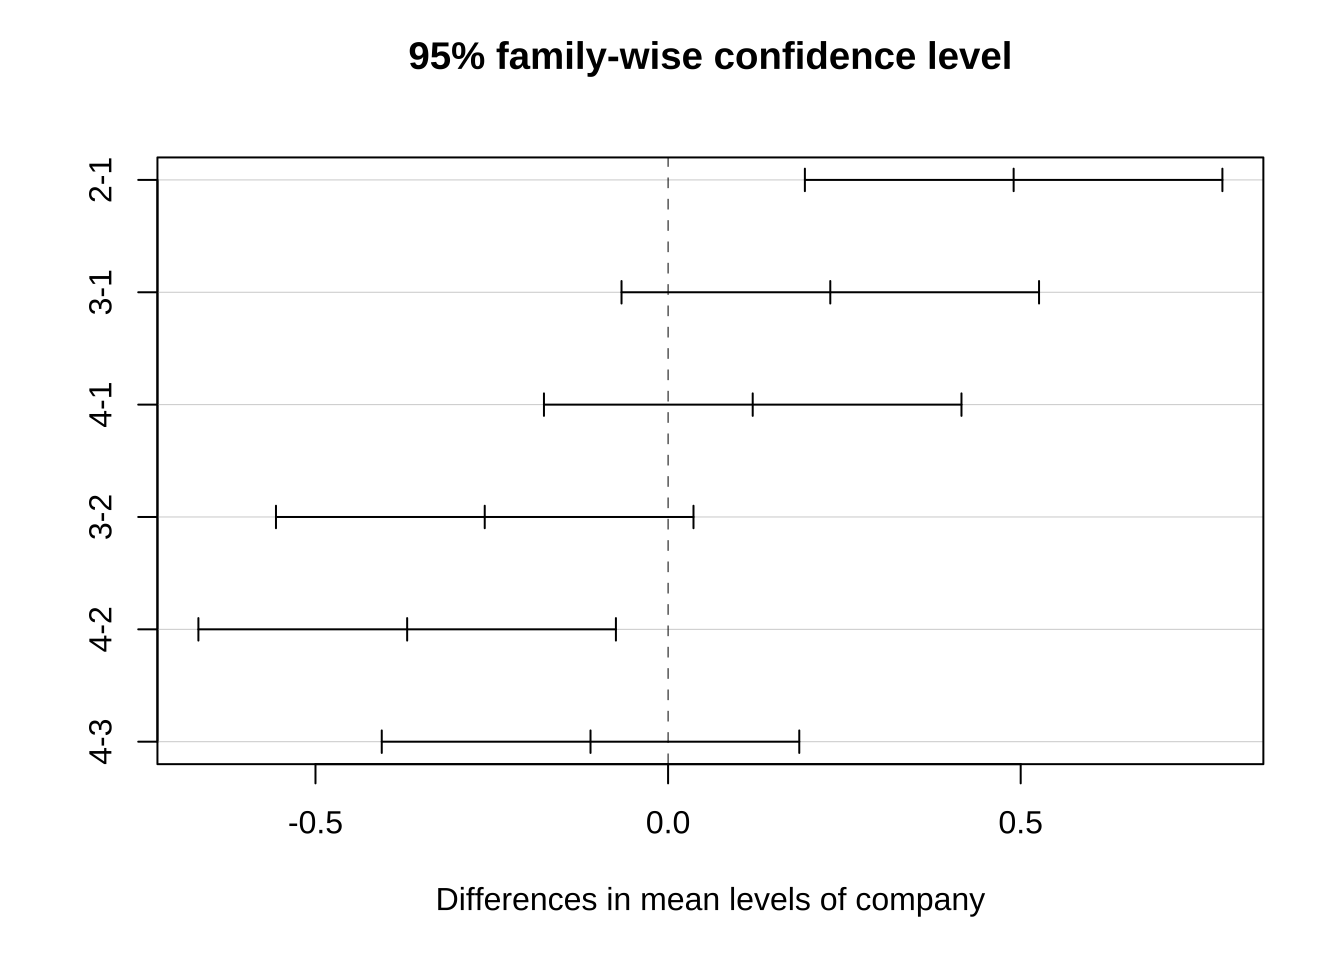
\includegraphics{lmpractice_files/figure-latex/unnamed-chunk-16-1.pdf}

\hypertarget{uxc911uxd68cuxadc0-uxbaa8uxd615uxc758-uxc801uxd569}{%
\section{중회귀 모형의 적합}\label{uxc911uxd68cuxadc0-uxbaa8uxd615uxc758-uxc801uxd569}}

\begin{Shaded}
\begin{Highlighting}[]
\NormalTok{fit0 }\OtherTok{\textless{}{-}} \FunctionTok{lm}\NormalTok{(price }\SpecialCharTok{\textasciitilde{}}\NormalTok{ year }\SpecialCharTok{+}\NormalTok{ mileage }\SpecialCharTok{+}\NormalTok{ cc }\SpecialCharTok{+}\NormalTok{ automatic, usedcars)}
\end{Highlighting}
\end{Shaded}

계획행렬은 다음과 같이 구할 수 있다.

\begin{Shaded}
\begin{Highlighting}[]
\FunctionTok{model.matrix}\NormalTok{(fit0)}
\end{Highlighting}
\end{Shaded}

\begin{verbatim}
##    (Intercept) year mileage   cc automatic
## 1            1   78  133462 1998         1
## 2            1   39   33000 2000         1
## 3            1  109  120000 1800         0
## 4            1   20   69727 1999         1
## 5            1   70  112000 2000         0
## 6            1   58   39106 1998         1
## 7            1   53   95935 1800         1
## 8            1   68  120000 1800         0
## 9            1   15   20215 1798         1
## 10           1   96  140000 1800         0
## 11           1   63   68924 1998         1
## 12           1   82   90000 2000         0
## 13           1   76   81279 1998         0
## 14           1   17   24070 1798         1
## 15           1   38   40000 2000         0
## 16           1   46   56887 1832         1
## 17           1   95   91216 1997         1
## 18           1   37   48680 1998         1
## 19           1   68    8000 2000         0
## 20           1   41   60634 1835         1
## 21           1   69  114131 1998         1
## 22           1   71   75000 1800         0
## 23           1   99  124417 1998         1
## 24           1  129  130000 1800         0
## 25           1   57   77559 1997         1
## 26           1  107   75216 1838         1
## 27           1   45   52000 2000         0
## 28           1   80   58000 2000         1
## 29           1  113  134500 1800         0
## 30           1   41   80000 2000         0
## attr(,"assign")
## [1] 0 1 2 3 4
\end{verbatim}

\texttt{fit0} 에 저장된 결과를 다음과 같이 함수 \texttt{str}을 이용하여 볼 수 있다.

\begin{Shaded}
\begin{Highlighting}[]
\FunctionTok{str}\NormalTok{(fit0)}
\end{Highlighting}
\end{Shaded}

\begin{verbatim}
## List of 12
##  $ coefficients : Named num [1:5] 525.28696 -5.79964 -0.00226 0.38879 165.31263
##   ..- attr(*, "names")= chr [1:5] "(Intercept)" "year" "mileage" "cc" ...
##  $ residuals    : Named num [1:30] 76.98 212.69 -51.4 -4.01 -53.45 ...
##   ..- attr(*, "names")= chr [1:30] "1" "2" "3" "4" ...
##  $ effects      : Named num [1:30] -4407 -1434 -369 -229 419 ...
##   ..- attr(*, "names")= chr [1:30] "(Intercept)" "year" "mileage" "cc" ...
##  $ rank         : int 5
##  $ fitted.values: Named num [1:30] 713 1167 321 1194 643 ...
##   ..- attr(*, "names")= chr [1:30] "1" "2" "3" "4" ...
##  $ assign       : int [1:5] 0 1 2 3 4
##  $ qr           :List of 5
##   ..$ qr   : num [1:30, 1:5] -5.477 0.183 0.183 0.183 0.183 ...
##   .. ..- attr(*, "dimnames")=List of 2
##   .. .. ..$ : chr [1:30] "1" "2" "3" "4" ...
##   .. .. ..$ : chr [1:5] "(Intercept)" "year" "mileage" "cc" ...
##   .. ..- attr(*, "assign")= int [1:5] 0 1 2 3 4
##   ..$ qraux: num [1:5] 1.18 1.18 1.08 1.03 1.26
##   ..$ pivot: int [1:5] 1 2 3 4 5
##   ..$ tol  : num 1e-07
##   ..$ rank : int 5
##   ..- attr(*, "class")= chr "qr"
##  $ df.residual  : int 25
##  $ xlevels      : Named list()
##  $ call         : language lm(formula = price ~ year + mileage + cc + automatic, data = usedcars)
##  $ terms        :Classes 'terms', 'formula'  language price ~ year + mileage + cc + automatic
##   .. ..- attr(*, "variables")= language list(price, year, mileage, cc, automatic)
##   .. ..- attr(*, "factors")= int [1:5, 1:4] 0 1 0 0 0 0 0 1 0 0 ...
##   .. .. ..- attr(*, "dimnames")=List of 2
##   .. .. .. ..$ : chr [1:5] "price" "year" "mileage" "cc" ...
##   .. .. .. ..$ : chr [1:4] "year" "mileage" "cc" "automatic"
##   .. ..- attr(*, "term.labels")= chr [1:4] "year" "mileage" "cc" "automatic"
##   .. ..- attr(*, "order")= int [1:4] 1 1 1 1
##   .. ..- attr(*, "intercept")= int 1
##   .. ..- attr(*, "response")= int 1
##   .. ..- attr(*, ".Environment")=<environment: R_GlobalEnv> 
##   .. ..- attr(*, "predvars")= language list(price, year, mileage, cc, automatic)
##   .. ..- attr(*, "dataClasses")= Named chr [1:5] "numeric" "numeric" "numeric" "numeric" ...
##   .. .. ..- attr(*, "names")= chr [1:5] "price" "year" "mileage" "cc" ...
##  $ model        :'data.frame':   30 obs. of  5 variables:
##   ..$ price    : int [1:30] 790 1380 270 1190 590 1120 815 450 1290 420 ...
##   ..$ year     : int [1:30] 78 39 109 20 70 58 53 68 15 96 ...
##   ..$ mileage  : int [1:30] 133462 33000 120000 69727 112000 39106 95935 120000 20215 140000 ...
##   ..$ cc       : int [1:30] 1998 2000 1800 1999 2000 1998 1800 1800 1798 1800 ...
##   ..$ automatic: int [1:30] 1 1 0 1 0 1 1 0 1 0 ...
##   ..- attr(*, "terms")=Classes 'terms', 'formula'  language price ~ year + mileage + cc + automatic
##   .. .. ..- attr(*, "variables")= language list(price, year, mileage, cc, automatic)
##   .. .. ..- attr(*, "factors")= int [1:5, 1:4] 0 1 0 0 0 0 0 1 0 0 ...
##   .. .. .. ..- attr(*, "dimnames")=List of 2
##   .. .. .. .. ..$ : chr [1:5] "price" "year" "mileage" "cc" ...
##   .. .. .. .. ..$ : chr [1:4] "year" "mileage" "cc" "automatic"
##   .. .. ..- attr(*, "term.labels")= chr [1:4] "year" "mileage" "cc" "automatic"
##   .. .. ..- attr(*, "order")= int [1:4] 1 1 1 1
##   .. .. ..- attr(*, "intercept")= int 1
##   .. .. ..- attr(*, "response")= int 1
##   .. .. ..- attr(*, ".Environment")=<environment: R_GlobalEnv> 
##   .. .. ..- attr(*, "predvars")= language list(price, year, mileage, cc, automatic)
##   .. .. ..- attr(*, "dataClasses")= Named chr [1:5] "numeric" "numeric" "numeric" "numeric" ...
##   .. .. .. ..- attr(*, "names")= chr [1:5] "price" "year" "mileage" "cc" ...
##  - attr(*, "class")= chr "lm"
\end{verbatim}

\hypertarget{uxd68cuxadc0uxacc4uxc218uxc758-uxcd94uxc815uxacfc-uxacb0uxc815uxacc4uxc218}{%
\section{회귀계수의 추정과 결정계수}\label{uxd68cuxadc0uxacc4uxc218uxc758-uxcd94uxc815uxacfc-uxacb0uxc815uxacc4uxc218}}

함수 \texttt{summary} 는 각 계수의 추정값과 가설 \(H_0: \beta_i=0\)에 대한 t-검정 결과를 보여준다.
또한 결정계수 \(R^2\)도 구해준다.

\begin{Shaded}
\begin{Highlighting}[]
\FunctionTok{summary}\NormalTok{(fit0)}
\end{Highlighting}
\end{Shaded}

\begin{verbatim}
## 
## Call:
## lm(formula = price ~ year + mileage + cc + automatic, data = usedcars)
## 
## Residuals:
##     Min      1Q  Median      3Q     Max 
## -177.35  -63.91   -0.99   70.34  212.69 
## 
## Coefficients:
##               Estimate Std. Error t value Pr(>|t|)    
## (Intercept)  5.253e+02  3.998e+02   1.314 0.200823    
## year        -5.800e+00  9.283e-01  -6.247 1.55e-06 ***
## mileage     -2.263e-03  7.211e-04  -3.138 0.004324 ** 
## cc           3.888e-01  2.022e-01   1.923 0.065958 .  
## automatic    1.653e+02  3.986e+01   4.147 0.000339 ***
## ---
## Signif. codes:  0 '***' 0.001 '**' 0.01 '*' 0.05 '.' 0.1 ' ' 1
## 
## Residual standard error: 101.1 on 25 degrees of freedom
## Multiple R-squared:  0.9045, Adjusted R-squared:  0.8892 
## F-statistic: 59.21 on 4 and 25 DF,  p-value: 2.184e-12
\end{verbatim}

각 회귀 계수에 대한 신뢰구간은 함수 \texttt{confint}로 구할 수 있다.

\begin{Shaded}
\begin{Highlighting}[]
\FunctionTok{confint}\NormalTok{(fit0)}
\end{Highlighting}
\end{Shaded}

\begin{verbatim}
##                     2.5 %        97.5 %
## (Intercept) -2.981256e+02  1.348699e+03
## year        -7.711605e+00 -3.887669e+00
## mileage     -3.748021e-03 -7.776672e-04
## cc          -2.763072e-02  8.052054e-01
## automatic    8.322275e+01  2.474025e+02
\end{verbatim}

공동 신뢰영역은 패키지 \texttt{ellipse} 에 있는 함수 \texttt{ellipse}를 이용해서 다음과 같이 그릴 수 있다.

\begin{Shaded}
\begin{Highlighting}[]
\FunctionTok{plot}\NormalTok{(ellipse}\SpecialCharTok{::}\FunctionTok{ellipse}\NormalTok{(fit0, }\AttributeTok{level =} \FloatTok{0.90}\NormalTok{), }\AttributeTok{type =} \StringTok{\textquotesingle{}l\textquotesingle{}}\NormalTok{)}
\end{Highlighting}
\end{Shaded}

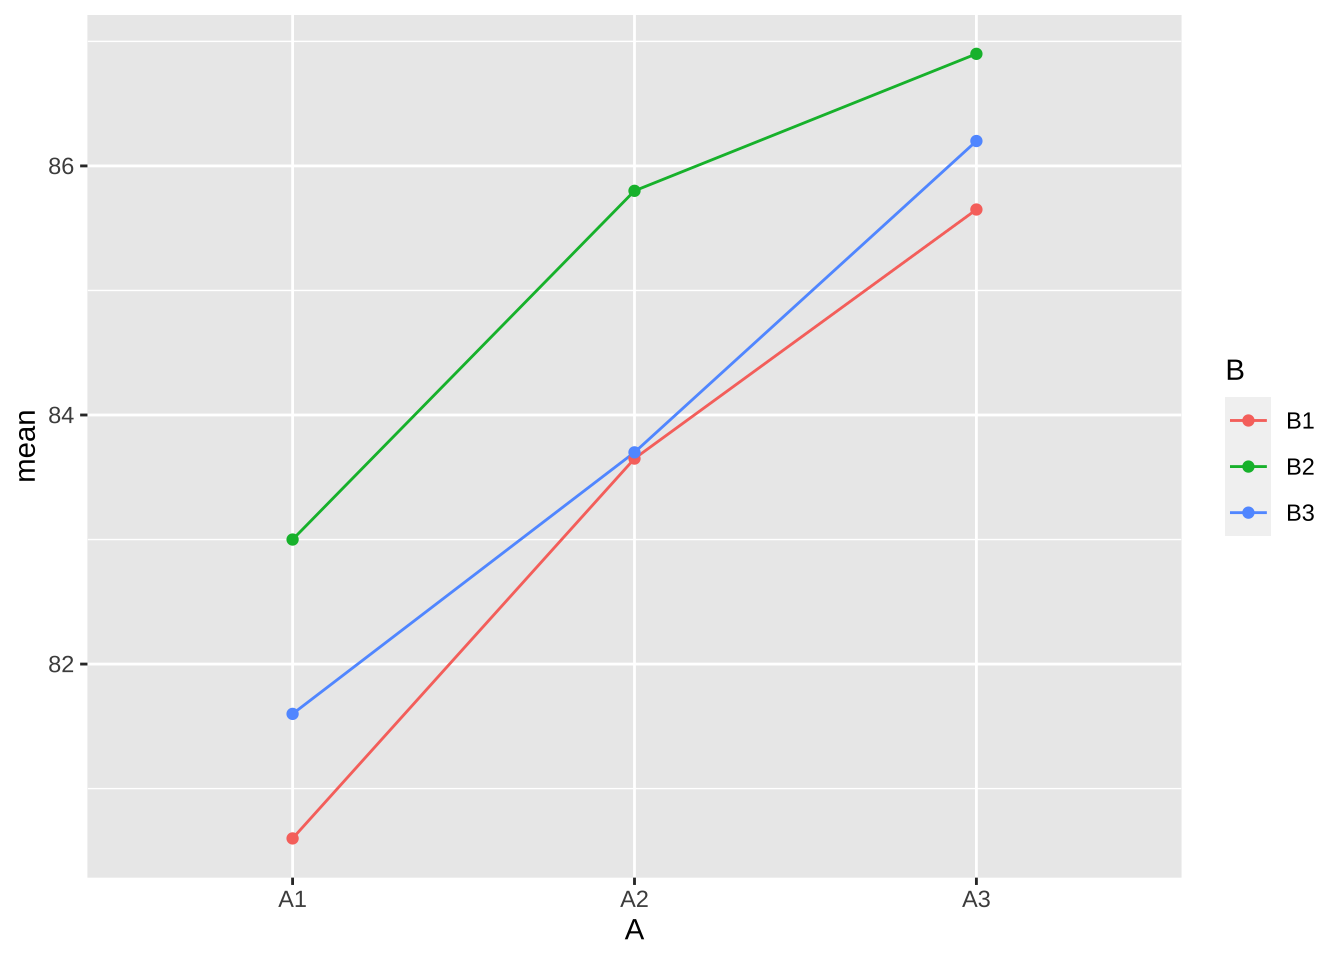
\includegraphics{lmpractice_files/figure-latex/unnamed-chunk-22-1.pdf}

\begin{Shaded}
\begin{Highlighting}[]
\FunctionTok{plot}\NormalTok{(ellipse}\SpecialCharTok{::}\FunctionTok{ellipse}\NormalTok{(fit0, }\AttributeTok{which =} \FunctionTok{c}\NormalTok{(}\StringTok{\textquotesingle{}year\textquotesingle{}}\NormalTok{, }\StringTok{\textquotesingle{}mileage\textquotesingle{}}\NormalTok{), }\AttributeTok{level =} \FloatTok{0.90}\NormalTok{), }\AttributeTok{type =} \StringTok{\textquotesingle{}l\textquotesingle{}}\NormalTok{)}
\FunctionTok{points}\NormalTok{(fit0}\SpecialCharTok{$}\NormalTok{coefficients[}\StringTok{\textquotesingle{}year\textquotesingle{}}\NormalTok{], fit0}\SpecialCharTok{$}\NormalTok{coefficients[}\StringTok{\textquotesingle{}mileage\textquotesingle{}}\NormalTok{])}
\end{Highlighting}
\end{Shaded}

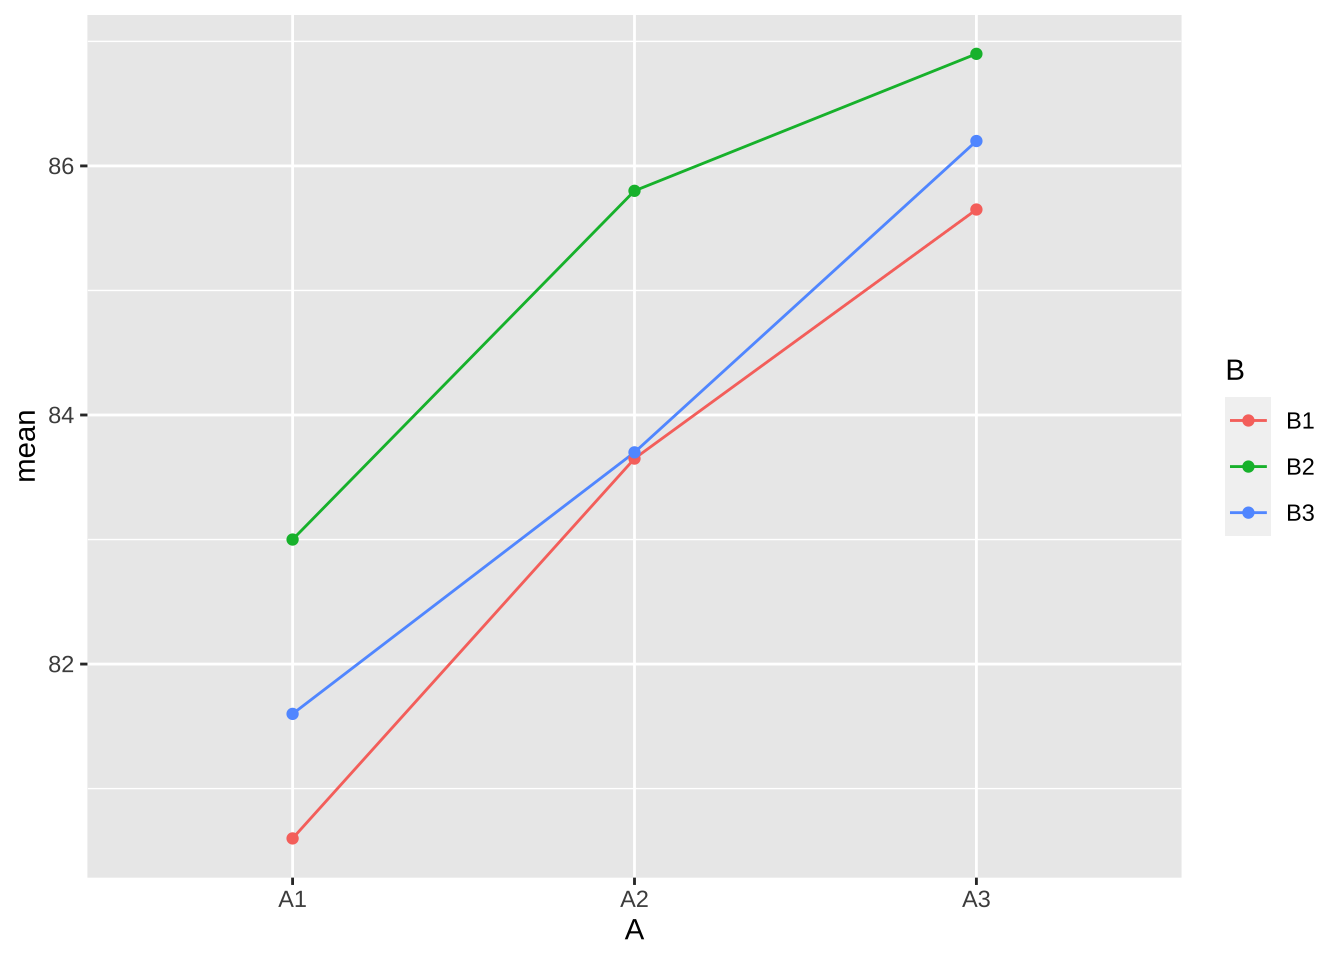
\includegraphics{lmpractice_files/figure-latex/unnamed-chunk-23-1.pdf}
\#\# 분산분석

\begin{Shaded}
\begin{Highlighting}[]
\FunctionTok{anova}\NormalTok{(fit0)}
\end{Highlighting}
\end{Shaded}

\begin{verbatim}
## Analysis of Variance Table
## 
## Response: price
##           Df  Sum Sq Mean Sq  F value    Pr(>F)    
## year       1 2056608 2056608 201.2036 1.841e-13 ***
## mileage    1  135864  135864  13.2919 0.0012228 ** 
## cc         1   52409   52409   5.1273 0.0324794 *  
## automatic  1  175828  175828  17.2018 0.0003389 ***
## Residuals 25  255538   10222                       
## ---
## Signif. codes:  0 '***' 0.001 '**' 0.01 '*' 0.05 '.' 0.1 ' ' 1
\end{verbatim}

\hypertarget{uxc608uxce21uxac12}{%
\section{예측값}\label{uxc608uxce21uxac12}}

반응변수에 대한 예측값 \(\hat {\bm y} = \bm X \hat {\bm \beta}\)는 함수 \texttt{redict}를 이용한다.

\begin{Shaded}
\begin{Highlighting}[]
\FunctionTok{predict}\NormalTok{(fit0)}
\end{Highlighting}
\end{Shaded}

\begin{verbatim}
##         1         2         3         4         5         6         7         8         9        10        11        12        13        14        15        16        17        18        19        20        21        22        23        24        25        26        27        28        29        30 
##  713.0214 1167.3146  321.4025 1194.0114  643.4485 1042.5270  865.9501  559.1876 1256.9013  351.5409  946.0553  623.6355  677.3900 1236.5788  991.9617 1007.3483  709.6348 1142.6549  890.3836 1029.0340  808.9611  643.6167  611.6964  182.7813  960.9247  614.4275  924.2101  872.9584  265.3927  884.0490
\end{verbatim}

새로운 자료에 대한 예측값 \(\widehat { E(y|x)}\)은 다음과 같이 데이터프레임을 만들고 예측한다.

\begin{Shaded}
\begin{Highlighting}[]
\NormalTok{nw }\OtherTok{\textless{}{-}} \FunctionTok{data.frame}\NormalTok{(}\AttributeTok{year=}\DecValTok{60}\NormalTok{, }\AttributeTok{mileage=}\DecValTok{10000}\NormalTok{, }\AttributeTok{cc=}\DecValTok{200}\NormalTok{, }\AttributeTok{automatic=}\DecValTok{1}\NormalTok{)}
\NormalTok{nw}
\end{Highlighting}
\end{Shaded}

\begin{verbatim}
##   year mileage  cc automatic
## 1   60   10000 200         1
\end{verbatim}

\begin{Shaded}
\begin{Highlighting}[]
\FunctionTok{predict}\NormalTok{(fit0, }\AttributeTok{newdata=}\NormalTok{nw, }\AttributeTok{interval=}\StringTok{"confidence"}\NormalTok{)}
\end{Highlighting}
\end{Shaded}

\begin{verbatim}
##        fit       lwr      upr
## 1 397.7504 -342.6272 1138.128
\end{verbatim}

새로운 관측값에 대항 예측은 다음과 같이 한다.

\begin{Shaded}
\begin{Highlighting}[]
\FunctionTok{predict}\NormalTok{(fit0, }\AttributeTok{newdata=}\NormalTok{nw, }\AttributeTok{interval=}\StringTok{"prediction"}\NormalTok{)}
\end{Highlighting}
\end{Shaded}

\begin{verbatim}
##        fit       lwr      upr
## 1 397.7504 -371.3501 1166.851
\end{verbatim}

\hypertarget{uxc794uxcc28-uxbd84uxc11d}{%
\section{잔차 분석}\label{uxc794uxcc28-uxbd84uxc11d}}

\begin{Shaded}
\begin{Highlighting}[]
\FunctionTok{plot}\NormalTok{(fit0)}
\end{Highlighting}
\end{Shaded}

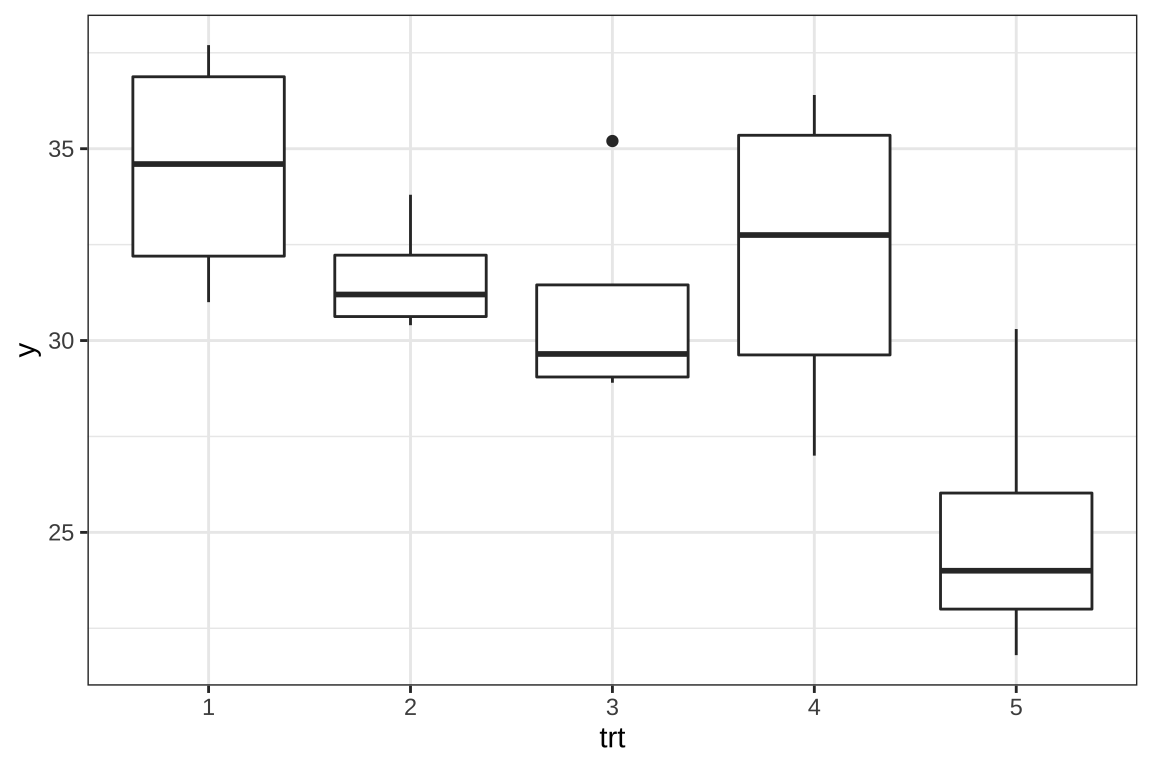
\includegraphics{lmpractice_files/figure-latex/unnamed-chunk-28-1.pdf} 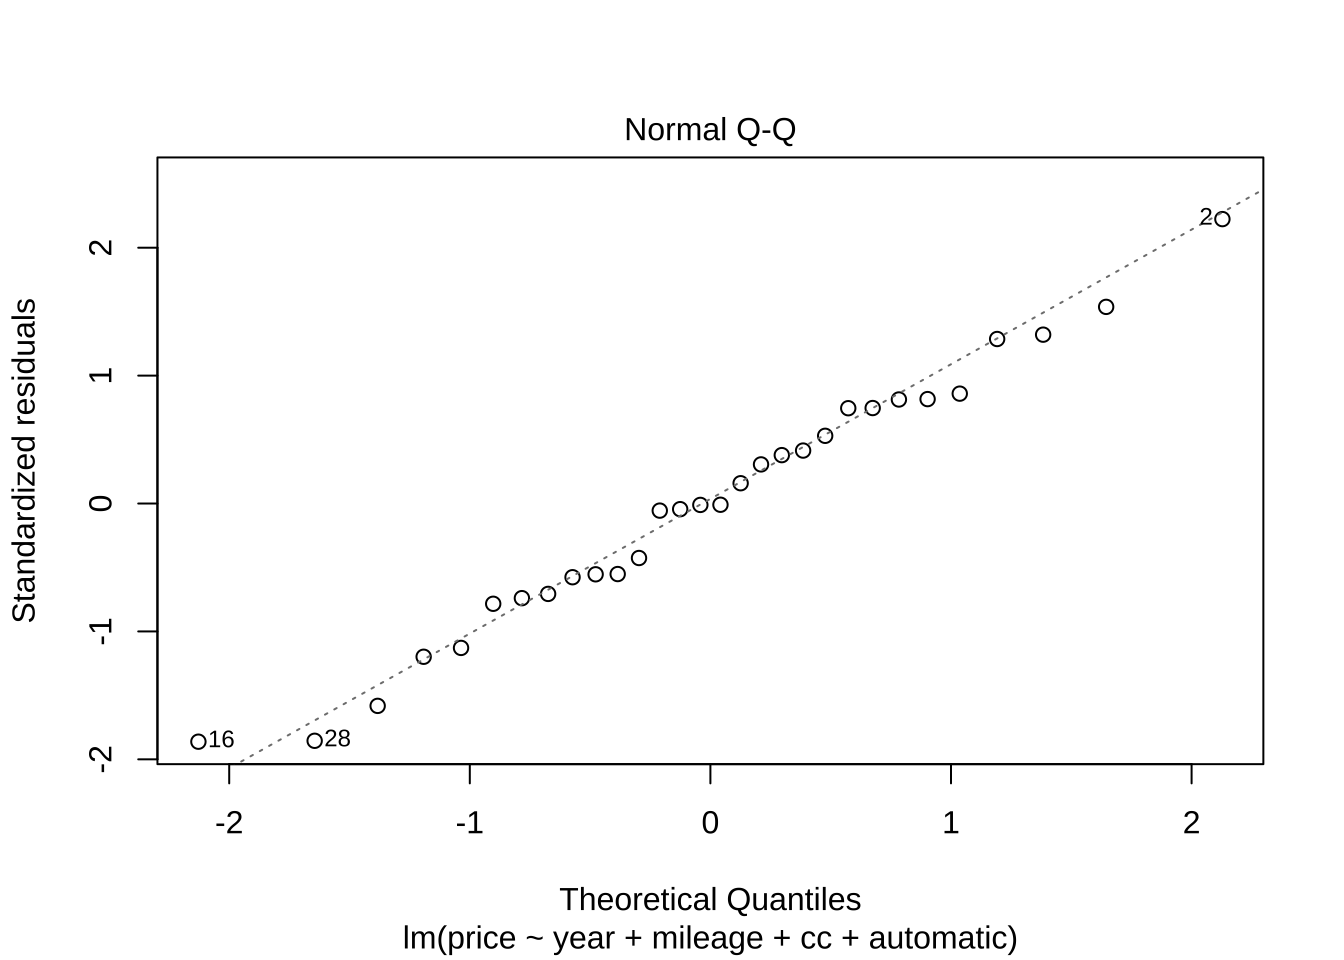
\includegraphics{lmpractice_files/figure-latex/unnamed-chunk-28-2.pdf} 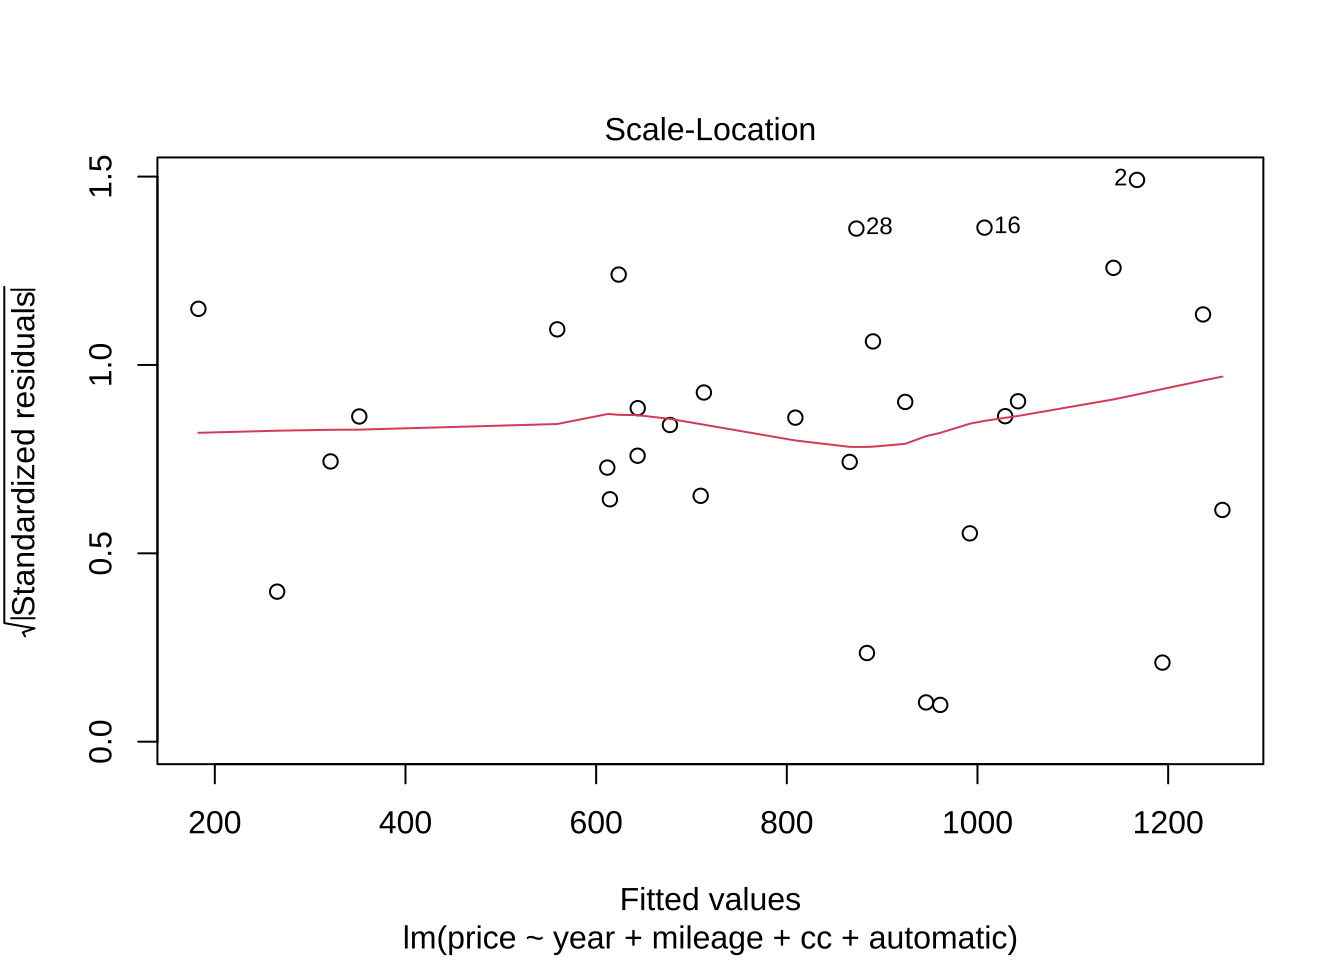
\includegraphics{lmpractice_files/figure-latex/unnamed-chunk-28-3.pdf} 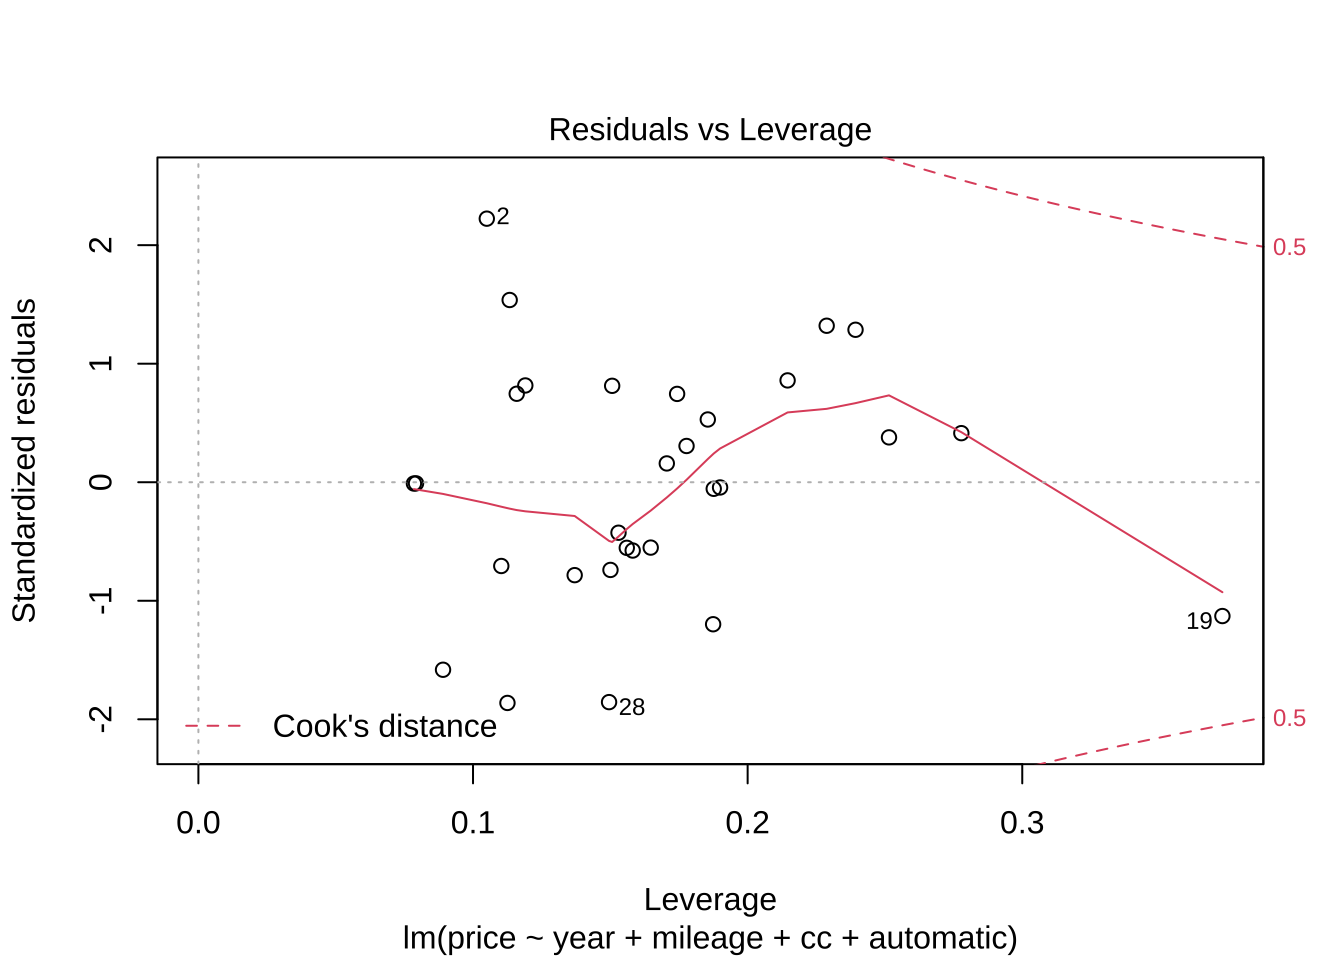
\includegraphics{lmpractice_files/figure-latex/unnamed-chunk-28-4.pdf}

\hypertarget{chapter04}{%
\chapter{모형의 진단과 수정}\label{chapter04}}

예제 3.3에 나온 중고차 가격자료를 이용한 R 실습입니다.

\hypertarget{uxc21cuxcc28uxc81cuxacf1uxd569}{%
\section{순차제곱합}\label{uxc21cuxcc28uxc81cuxacf1uxd569}}

순차제곱합은 모형에 들어가는 변수의 순서에 따라서 제곱합이 틀려진다.

다음의 예를 보면 두 모형이 같은 변수들로 적합되지만 순서가 달라지면 순차제곱합이 다르다.

\begin{Shaded}
\begin{Highlighting}[]
\NormalTok{model1 }\OtherTok{\textless{}{-}}\NormalTok{ price }\SpecialCharTok{\textasciitilde{}}\NormalTok{ year }\SpecialCharTok{+}\NormalTok{ mileage }\SpecialCharTok{+}\NormalTok{ cc }\SpecialCharTok{+}\NormalTok{ automatic}
\NormalTok{model2 }\OtherTok{\textless{}{-}}\NormalTok{ price }\SpecialCharTok{\textasciitilde{}}\NormalTok{ mileage }\SpecialCharTok{+}\NormalTok{ automatic }\SpecialCharTok{+}\NormalTok{ cc }\SpecialCharTok{+}\NormalTok{ year}
\NormalTok{fit1 }\OtherTok{\textless{}{-}} \FunctionTok{lm}\NormalTok{(model1, usedcars)}
\NormalTok{fit2 }\OtherTok{\textless{}{-}} \FunctionTok{lm}\NormalTok{(model2, usedcars)}
\FunctionTok{anova}\NormalTok{(fit1)}
\end{Highlighting}
\end{Shaded}

\begin{verbatim}
## Analysis of Variance Table
## 
## Response: price
##           Df  Sum Sq Mean Sq  F value    Pr(>F)    
## year       1 2056608 2056608 201.2036 1.841e-13 ***
## mileage    1  135864  135864  13.2919 0.0012228 ** 
## cc         1   52409   52409   5.1273 0.0324794 *  
## automatic  1  175828  175828  17.2018 0.0003389 ***
## Residuals 25  255538   10222                       
## ---
## Signif. codes:  0 '***' 0.001 '**' 0.01 '*' 0.05 '.' 0.1 ' ' 1
\end{verbatim}

\begin{Shaded}
\begin{Highlighting}[]
\FunctionTok{anova}\NormalTok{(fit2)}
\end{Highlighting}
\end{Shaded}

\begin{verbatim}
## Analysis of Variance Table
## 
## Response: price
##           Df  Sum Sq Mean Sq  F value    Pr(>F)    
## mileage    1 1637355 1637355 160.1870 2.274e-12 ***
## automatic  1  341741  341741  33.4335 5.006e-06 ***
## cc         1   42683   42683   4.1758   0.05168 .  
## year       1  398929  398929  39.0283 1.552e-06 ***
## Residuals 25  255538   10222                       
## ---
## Signif. codes:  0 '***' 0.001 '**' 0.01 '*' 0.05 '.' 0.1 ' ' 1
\end{verbatim}

하지만 회귀계수의 추정량은 동일하다.

\begin{Shaded}
\begin{Highlighting}[]
\FunctionTok{summary}\NormalTok{(fit1)}
\end{Highlighting}
\end{Shaded}

\begin{verbatim}
## 
## Call:
## lm(formula = model1, data = usedcars)
## 
## Residuals:
##     Min      1Q  Median      3Q     Max 
## -177.35  -63.91   -0.99   70.34  212.69 
## 
## Coefficients:
##               Estimate Std. Error t value Pr(>|t|)    
## (Intercept)  5.253e+02  3.998e+02   1.314 0.200823    
## year        -5.800e+00  9.283e-01  -6.247 1.55e-06 ***
## mileage     -2.263e-03  7.211e-04  -3.138 0.004324 ** 
## cc           3.888e-01  2.022e-01   1.923 0.065958 .  
## automatic    1.653e+02  3.986e+01   4.147 0.000339 ***
## ---
## Signif. codes:  0 '***' 0.001 '**' 0.01 '*' 0.05 '.' 0.1 ' ' 1
## 
## Residual standard error: 101.1 on 25 degrees of freedom
## Multiple R-squared:  0.9045, Adjusted R-squared:  0.8892 
## F-statistic: 59.21 on 4 and 25 DF,  p-value: 2.184e-12
\end{verbatim}

\begin{Shaded}
\begin{Highlighting}[]
\FunctionTok{summary}\NormalTok{(fit2)}
\end{Highlighting}
\end{Shaded}

\begin{verbatim}
## 
## Call:
## lm(formula = model2, data = usedcars)
## 
## Residuals:
##     Min      1Q  Median      3Q     Max 
## -177.35  -63.91   -0.99   70.34  212.69 
## 
## Coefficients:
##               Estimate Std. Error t value Pr(>|t|)    
## (Intercept)  5.253e+02  3.998e+02   1.314 0.200823    
## mileage     -2.263e-03  7.211e-04  -3.138 0.004324 ** 
## automatic    1.653e+02  3.986e+01   4.147 0.000339 ***
## cc           3.888e-01  2.022e-01   1.923 0.065958 .  
## year        -5.800e+00  9.283e-01  -6.247 1.55e-06 ***
## ---
## Signif. codes:  0 '***' 0.001 '**' 0.01 '*' 0.05 '.' 0.1 ' ' 1
## 
## Residual standard error: 101.1 on 25 degrees of freedom
## Multiple R-squared:  0.9045, Adjusted R-squared:  0.8892 
## F-statistic: 59.21 on 4 and 25 DF,  p-value: 2.184e-12
\end{verbatim}

\hypertarget{uxd3b8uxc81cuxacf1uxd569}{%
\section{편제곱합}\label{uxd3b8uxc81cuxacf1uxd569}}

편제곱합은 다른 변수들로 보정된 제곱합으로 순서에 관계없이 일정하다.패키지 \texttt{car} 에 있는 함수 \texttt{Anova} 를 사용하면
편제곱합을 구할 수 있다.

\begin{Shaded}
\begin{Highlighting}[]
\FunctionTok{Anova}\NormalTok{(fit1, }\AttributeTok{type=}\StringTok{"III"}\NormalTok{)}
\end{Highlighting}
\end{Shaded}

\begin{verbatim}
## Anova Table (Type III tests)
## 
## Response: price
##             Sum Sq Df F value    Pr(>F)    
## (Intercept)  17645  1  1.7262 0.2008228    
## year        398929  1 39.0283 1.552e-06 ***
## mileage     100649  1  9.8467 0.0043244 ** 
## cc           37794  1  3.6975 0.0659577 .  
## automatic   175828  1 17.2018 0.0003389 ***
## Residuals   255538 25                      
## ---
## Signif. codes:  0 '***' 0.001 '**' 0.01 '*' 0.05 '.' 0.1 ' ' 1
\end{verbatim}

\begin{Shaded}
\begin{Highlighting}[]
\FunctionTok{Anova}\NormalTok{(fit2, }\AttributeTok{type=}\StringTok{"III"}\NormalTok{)}
\end{Highlighting}
\end{Shaded}

\begin{verbatim}
## Anova Table (Type III tests)
## 
## Response: price
##             Sum Sq Df F value    Pr(>F)    
## (Intercept)  17645  1  1.7262 0.2008228    
## mileage     100649  1  9.8467 0.0043244 ** 
## automatic   175828  1 17.2018 0.0003389 ***
## cc           37794  1  3.6975 0.0659577 .  
## year        398929  1 39.0283 1.552e-06 ***
## Residuals   255538 25                      
## ---
## Signif. codes:  0 '***' 0.001 '**' 0.01 '*' 0.05 '.' 0.1 ' ' 1
\end{verbatim}

\hypertarget{uxbd80uxbd84-f-uxac80uxc815}{%
\section{부분 F 검정}\label{uxbd80uxbd84-f-uxac80uxc815}}

배기량(cc)에 대항 계수가 0인지 검정해보자.

\[ H_0: ~ \beta_k =0 \]

하나의 계수에 대한 검정은 분산분석 표의 t-검정으로도 가능하며 결과는 동일하다.

\begin{Shaded}
\begin{Highlighting}[]
\NormalTok{fullmodel }\OtherTok{\textless{}{-}}\NormalTok{ price }\SpecialCharTok{\textasciitilde{}}\NormalTok{ year }\SpecialCharTok{+}\NormalTok{ mileage }\SpecialCharTok{+}\NormalTok{ cc }\SpecialCharTok{+}\NormalTok{ automatic}
\NormalTok{reducemodel1 }\OtherTok{\textless{}{-}}\NormalTok{ price }\SpecialCharTok{\textasciitilde{}}\NormalTok{ year }\SpecialCharTok{+}\NormalTok{ mileage }\SpecialCharTok{+}\NormalTok{ automatic}
\NormalTok{fitfull }\OtherTok{\textless{}{-}} \FunctionTok{lm}\NormalTok{(fullmodel, }\AttributeTok{data=}\NormalTok{usedcars)}
\NormalTok{fitreduce1 }\OtherTok{\textless{}{-}} \FunctionTok{lm}\NormalTok{(reducemodel1, }\AttributeTok{data=}\NormalTok{usedcars)}
\FunctionTok{anova}\NormalTok{(fitreduce1, fitfull)}
\end{Highlighting}
\end{Shaded}

\begin{verbatim}
## Analysis of Variance Table
## 
## Model 1: price ~ year + mileage + automatic
## Model 2: price ~ year + mileage + cc + automatic
##   Res.Df    RSS Df Sum of Sq      F  Pr(>F)  
## 1     26 293332                              
## 2     25 255538  1     37794 3.6975 0.06596 .
## ---
## Signif. codes:  0 '***' 0.001 '**' 0.01 '*' 0.05 '.' 0.1 ' ' 1
\end{verbatim}

이제 두 개 이상
의 변수에 대하여 부분 F 검정을 해보자.

\begin{Shaded}
\begin{Highlighting}[]
\NormalTok{reducemodel2 }\OtherTok{\textless{}{-}}\NormalTok{ price }\SpecialCharTok{\textasciitilde{}}\NormalTok{ year }\SpecialCharTok{+}\NormalTok{ mileage}
\NormalTok{fitreduce2 }\OtherTok{\textless{}{-}} \FunctionTok{lm}\NormalTok{(reducemodel2, }\AttributeTok{data=}\NormalTok{usedcars)}
\FunctionTok{anova}\NormalTok{(fitreduce2, fitfull)}
\end{Highlighting}
\end{Shaded}

\begin{verbatim}
## Analysis of Variance Table
## 
## Model 1: price ~ year + mileage
## Model 2: price ~ year + mileage + cc + automatic
##   Res.Df    RSS Df Sum of Sq      F    Pr(>F)    
## 1     27 483775                                  
## 2     25 255538  2    228237 11.165 0.0003429 ***
## ---
## Signif. codes:  0 '***' 0.001 '**' 0.01 '*' 0.05 '.' 0.1 ' ' 1
\end{verbatim}

\hypertarget{uxc120uxd615-uxac00uxc124uxc5d0-uxb300uxd55c-uxac80uxc815}{%
\section{선형 가설에 대한 검정}\label{uxc120uxd615-uxac00uxc124uxc5d0-uxb300uxd55c-uxac80uxc815}}

다음과 같은 선형 가설을 생각자.

\[ H_0: \bm L \bm \beta= \bm 0\]

예제 4.4 에서 다음과 같은 가설을 고려한다.

\[ H_0: \beta_2=0, \beta_3= 2.5 \beta_4 \]

\begin{Shaded}
\begin{Highlighting}[]
\NormalTok{modreduce }\OtherTok{\textless{}{-}} \FunctionTok{lm}\NormalTok{(suneung }\SpecialCharTok{\textasciitilde{}}\NormalTok{ kor }\SpecialCharTok{+} \FunctionTok{I}\NormalTok{(}\FloatTok{2.5}\SpecialCharTok{*}\NormalTok{math }\SpecialCharTok{+}\NormalTok{ sci), }\AttributeTok{data=}\NormalTok{suneung)}
\NormalTok{modfull }\OtherTok{\textless{}{-}} \FunctionTok{lm}\NormalTok{(suneung }\SpecialCharTok{\textasciitilde{}}\NormalTok{ kor }\SpecialCharTok{+}\NormalTok{ eng }\SpecialCharTok{+}\NormalTok{ math }\SpecialCharTok{+}\NormalTok{ sci, }\AttributeTok{data=}\NormalTok{suneung)}
\FunctionTok{anova}\NormalTok{(modreduce, modfull)}
\end{Highlighting}
\end{Shaded}

\begin{verbatim}
## Analysis of Variance Table
## 
## Model 1: suneung ~ kor + I(2.5 * math + sci)
## Model 2: suneung ~ kor + eng + math + sci
##   Res.Df    RSS Df Sum of Sq      F Pr(>F)
## 1     22 3136.4                           
## 2     20 3023.5  2    112.95 0.3736  0.693
\end{verbatim}

위의 검정은 다음과 과 같이 선형행렬 \(L\)을 정의하고 함수 \texttt{car::linearHypothesis}를 이용한 결과와 같다.

\[
H_0: 
\begin{bmatrix}
0 & 0  & 1 & 0 & 0  \\
0 & 0  & 0 & 1 &-2.5 
\end{bmatrix}
\begin{bmatrix}
\beta_0 \\
\beta_1 \\
\beta_2 \\
\beta_3 \\
\beta_4 
\end{bmatrix}
=\bm 0
\]

\begin{Shaded}
\begin{Highlighting}[]
\NormalTok{L }\OtherTok{\textless{}{-}} \FunctionTok{matrix}\NormalTok{(}\FunctionTok{c}\NormalTok{(}\DecValTok{0}\NormalTok{,}\DecValTok{0}\NormalTok{,}\DecValTok{1}\NormalTok{,}\DecValTok{0}\NormalTok{,}\DecValTok{0}\NormalTok{,}\DecValTok{0}\NormalTok{,}\DecValTok{0}\NormalTok{,}\DecValTok{0}\NormalTok{,}\DecValTok{1}\NormalTok{,}\SpecialCharTok{{-}}\FloatTok{2.5}\NormalTok{),}\DecValTok{2}\NormalTok{,}\DecValTok{5}\NormalTok{, }\AttributeTok{byrow=}\ConstantTok{TRUE}\NormalTok{)}
\NormalTok{L}
\end{Highlighting}
\end{Shaded}

\begin{verbatim}
##      [,1] [,2] [,3] [,4] [,5]
## [1,]    0    0    1    0  0.0
## [2,]    0    0    0    1 -2.5
\end{verbatim}

\begin{Shaded}
\begin{Highlighting}[]
\FunctionTok{linearHypothesis}\NormalTok{(modfull, }\AttributeTok{hypothesis.matrix=}\NormalTok{L)}
\end{Highlighting}
\end{Shaded}

\begin{verbatim}
## Linear hypothesis test
## 
## Hypothesis:
## eng = 0
## math - 2.5 sci = 0
## 
## Model 1: restricted model
## Model 2: suneung ~ kor + eng + math + sci
## 
##   Res.Df    RSS Df Sum of Sq      F Pr(>F)
## 1     22 3136.4                           
## 2     20 3023.5  2    112.95 0.3736  0.693
\end{verbatim}

\hypertarget{uxbcc0uxc218uxbcc0uxd658}{%
\section{변수변환}\label{uxbcc0uxc218uxbcc0uxd658}}

로그변화을 고려해 보자.

\begin{Shaded}
\begin{Highlighting}[]
\FunctionTok{plot}\NormalTok{(y}\SpecialCharTok{\textasciitilde{}}\NormalTok{time, regbook}\SpecialCharTok{::}\NormalTok{bug)}
\end{Highlighting}
\end{Shaded}

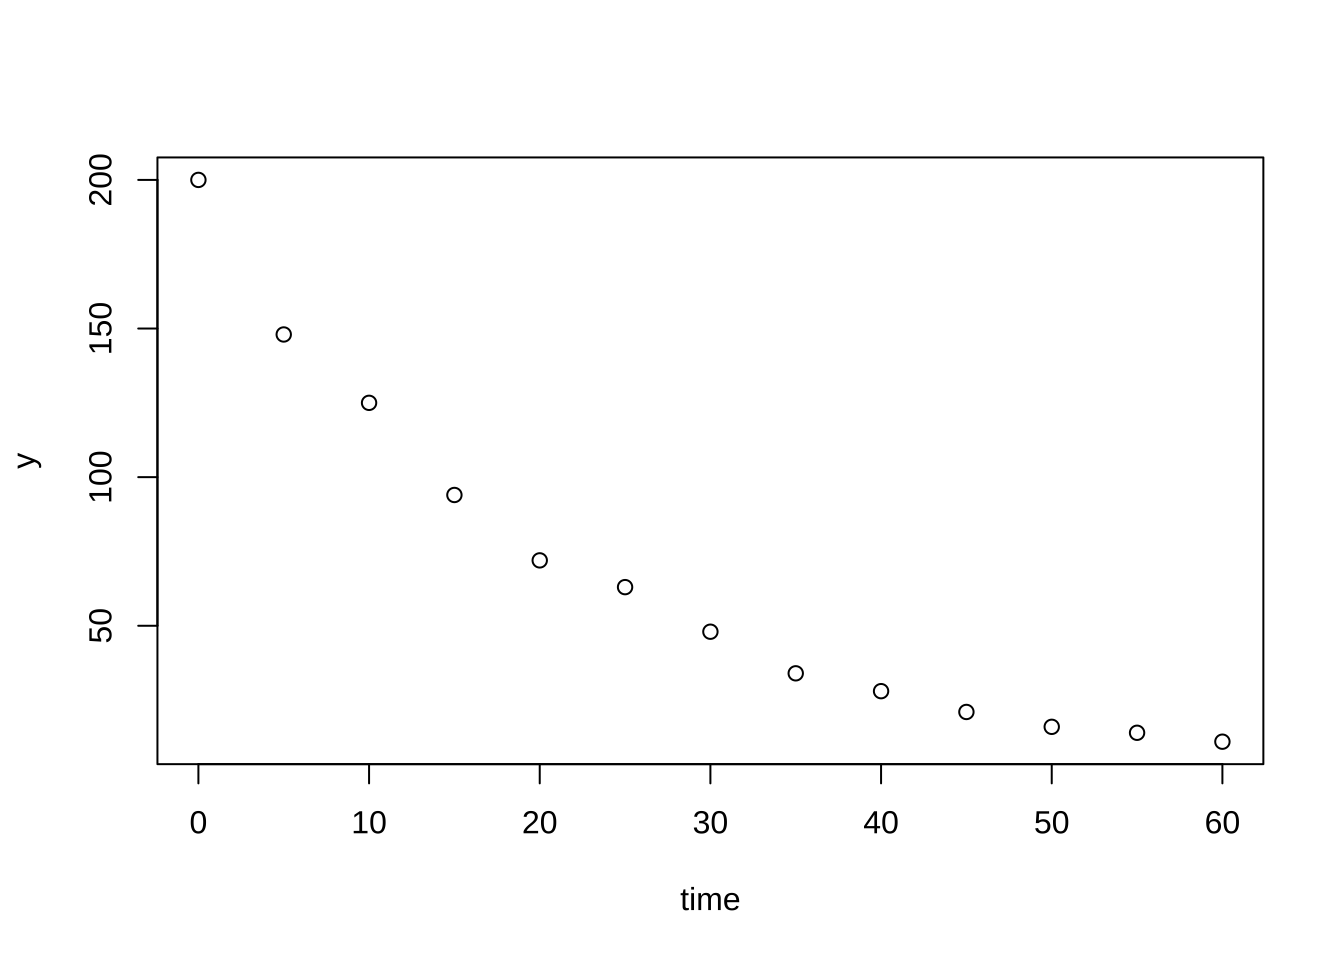
\includegraphics{lmpractice_files/figure-latex/unnamed-chunk-36-1.pdf}

\begin{Shaded}
\begin{Highlighting}[]
\NormalTok{bug2 }\OtherTok{\textless{}{-}}\NormalTok{regbook}\SpecialCharTok{::}\NormalTok{bug}
\NormalTok{bug2}\SpecialCharTok{$}\NormalTok{logy }\OtherTok{\textless{}{-}} \FunctionTok{log}\NormalTok{(bug2}\SpecialCharTok{$}\NormalTok{y)}
\NormalTok{fitlog }\OtherTok{\textless{}{-}} \FunctionTok{lm}\NormalTok{(logy}\SpecialCharTok{\textasciitilde{}}\NormalTok{time, bug2)}
\FunctionTok{plot}\NormalTok{(logy}\SpecialCharTok{\textasciitilde{}}\NormalTok{time, bug2)}
\FunctionTok{abline}\NormalTok{(fitlog)}
\end{Highlighting}
\end{Shaded}

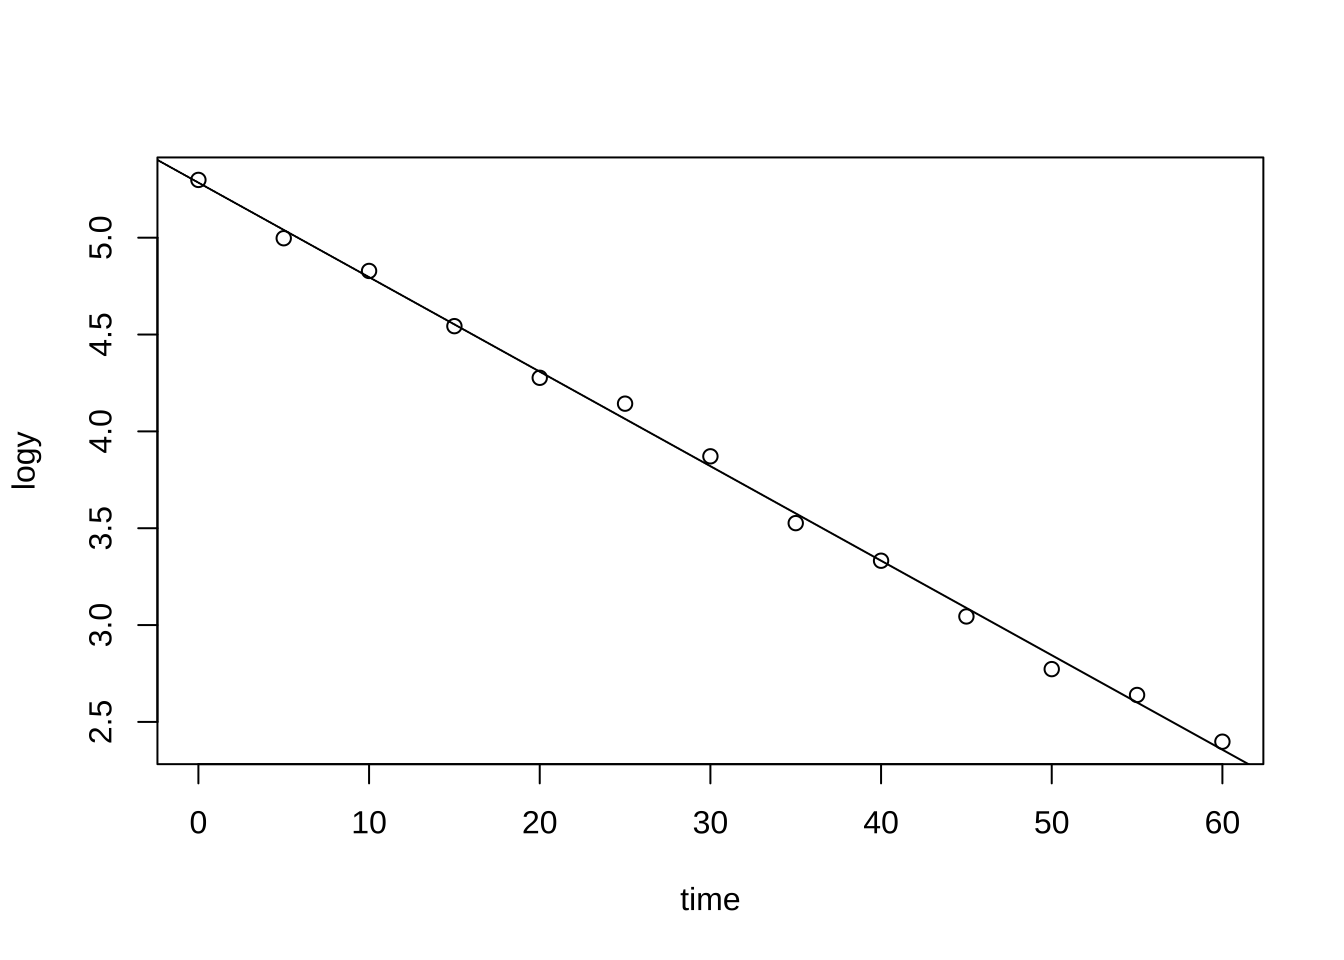
\includegraphics{lmpractice_files/figure-latex/unnamed-chunk-36-2.pdf}

Box-Cox 변환은 다음과 같이 수행한다. 패키지 \texttt{MASS} 의 함수 \texttt{boxcox} 를 이용한다.

\begin{itemize}
\tightlist
\item
  \texttt{foot}:발길이(mm), 양말을 벗은 상태로 측정하였고 오른쪽 발만 측정하였다.
\item
  \texttt{forearm}: 팔안쪽길이(mm), 손목부터 팔꿈치가 접히는 부분까지의 길이이다. 오른쪽 팔만 측정하였다.
\end{itemize}

\begin{Shaded}
\begin{Highlighting}[]
\FunctionTok{plot}\NormalTok{(foot }\SpecialCharTok{\textasciitilde{}}\NormalTok{ forearm, }\AttributeTok{data=}\NormalTok{aflength)}
\end{Highlighting}
\end{Shaded}

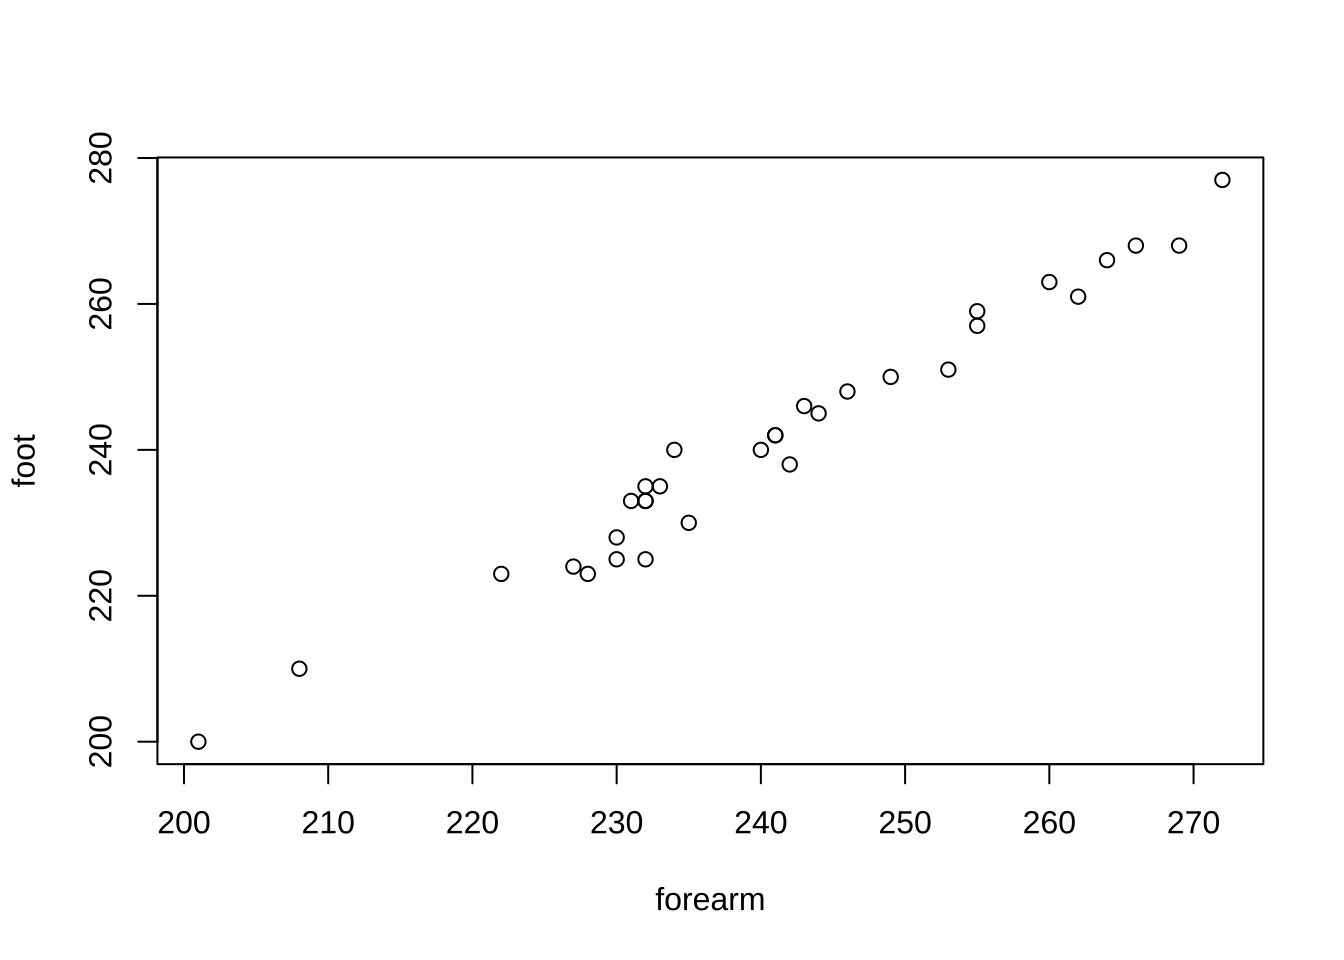
\includegraphics{lmpractice_files/figure-latex/unnamed-chunk-37-1.pdf}

\begin{Shaded}
\begin{Highlighting}[]
\FunctionTok{boxcox}\NormalTok{(}\FunctionTok{lm}\NormalTok{(foot }\SpecialCharTok{\textasciitilde{}}\NormalTok{ forearm, }\AttributeTok{data=}\NormalTok{aflength))}
\end{Highlighting}
\end{Shaded}

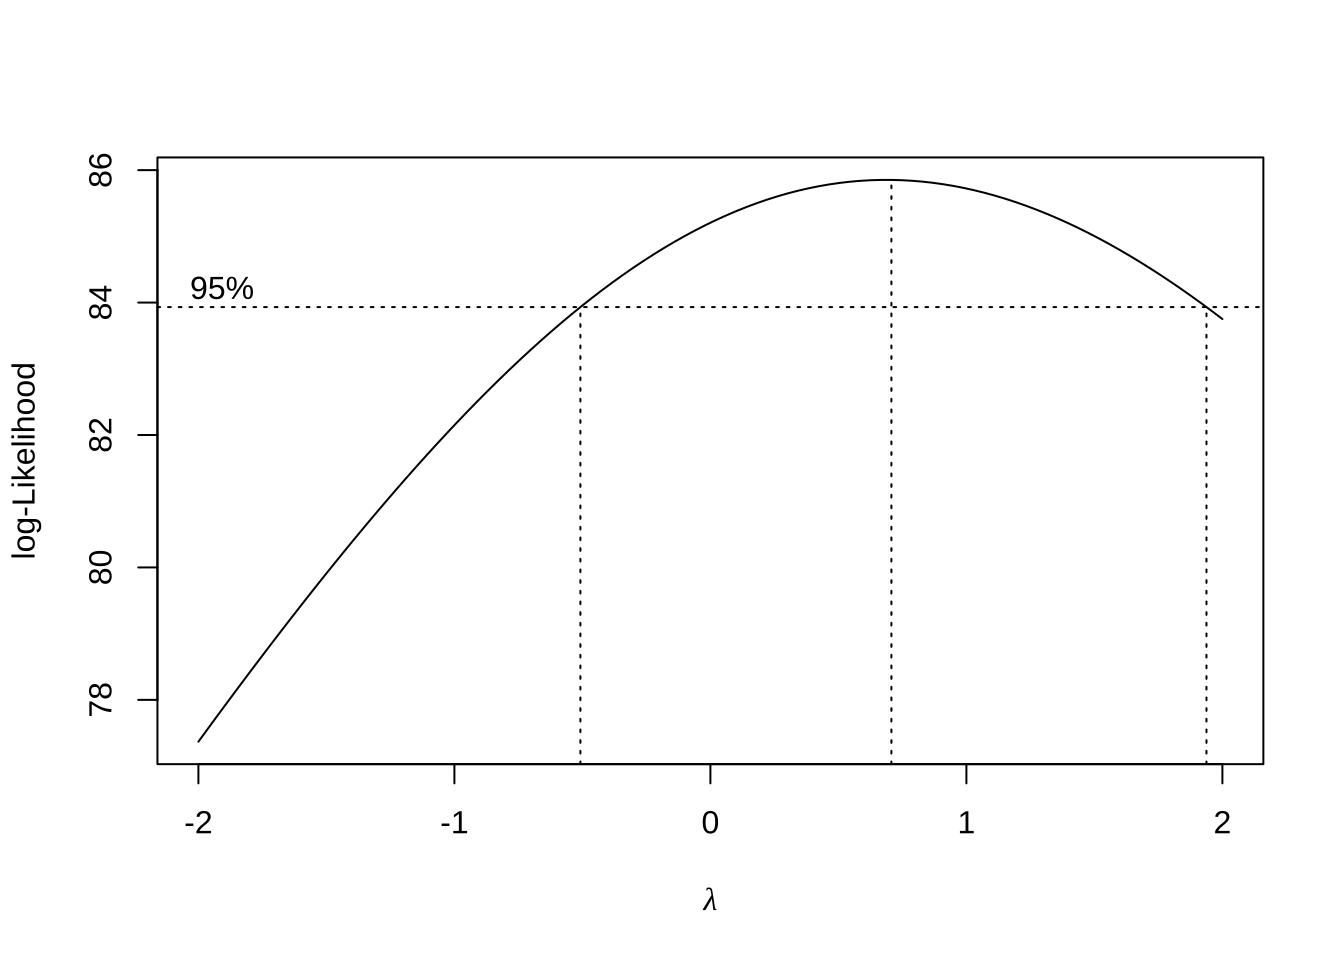
\includegraphics{lmpractice_files/figure-latex/unnamed-chunk-37-2.pdf}
- 예제 4.11

\begin{Shaded}
\begin{Highlighting}[]
\NormalTok{woolfm1 }\OtherTok{\textless{}{-}} \FunctionTok{lm}\NormalTok{(cycle}\SpecialCharTok{\textasciitilde{}}\NormalTok{length }\SpecialCharTok{+}\NormalTok{ amplitude }\SpecialCharTok{+}\NormalTok{ load, }\AttributeTok{data=}\NormalTok{wool)}
\FunctionTok{plot}\NormalTok{(woolfm1)}
\end{Highlighting}
\end{Shaded}

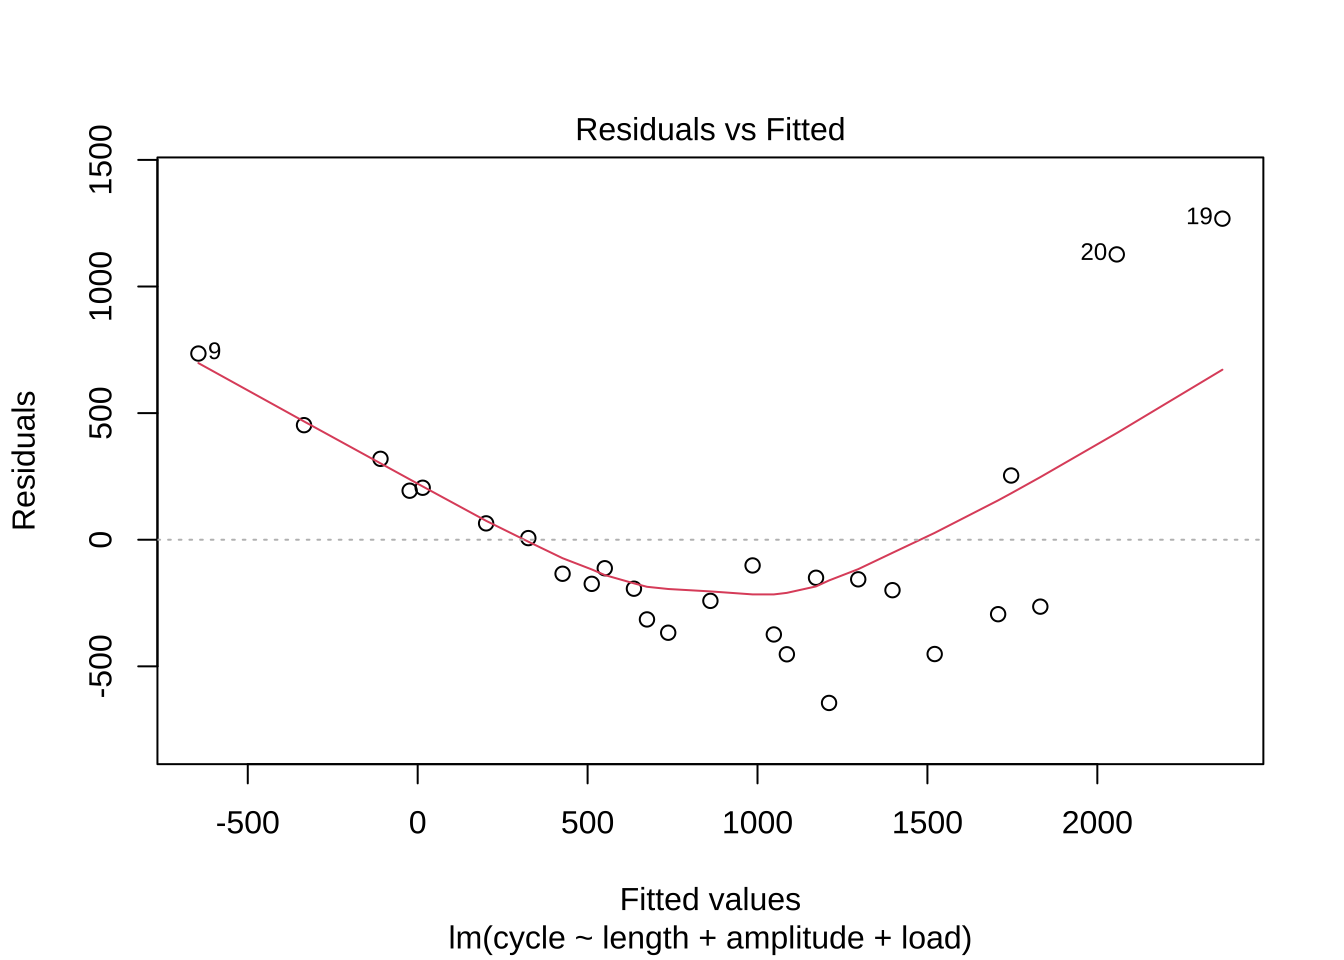
\includegraphics{lmpractice_files/figure-latex/unnamed-chunk-38-1.pdf} 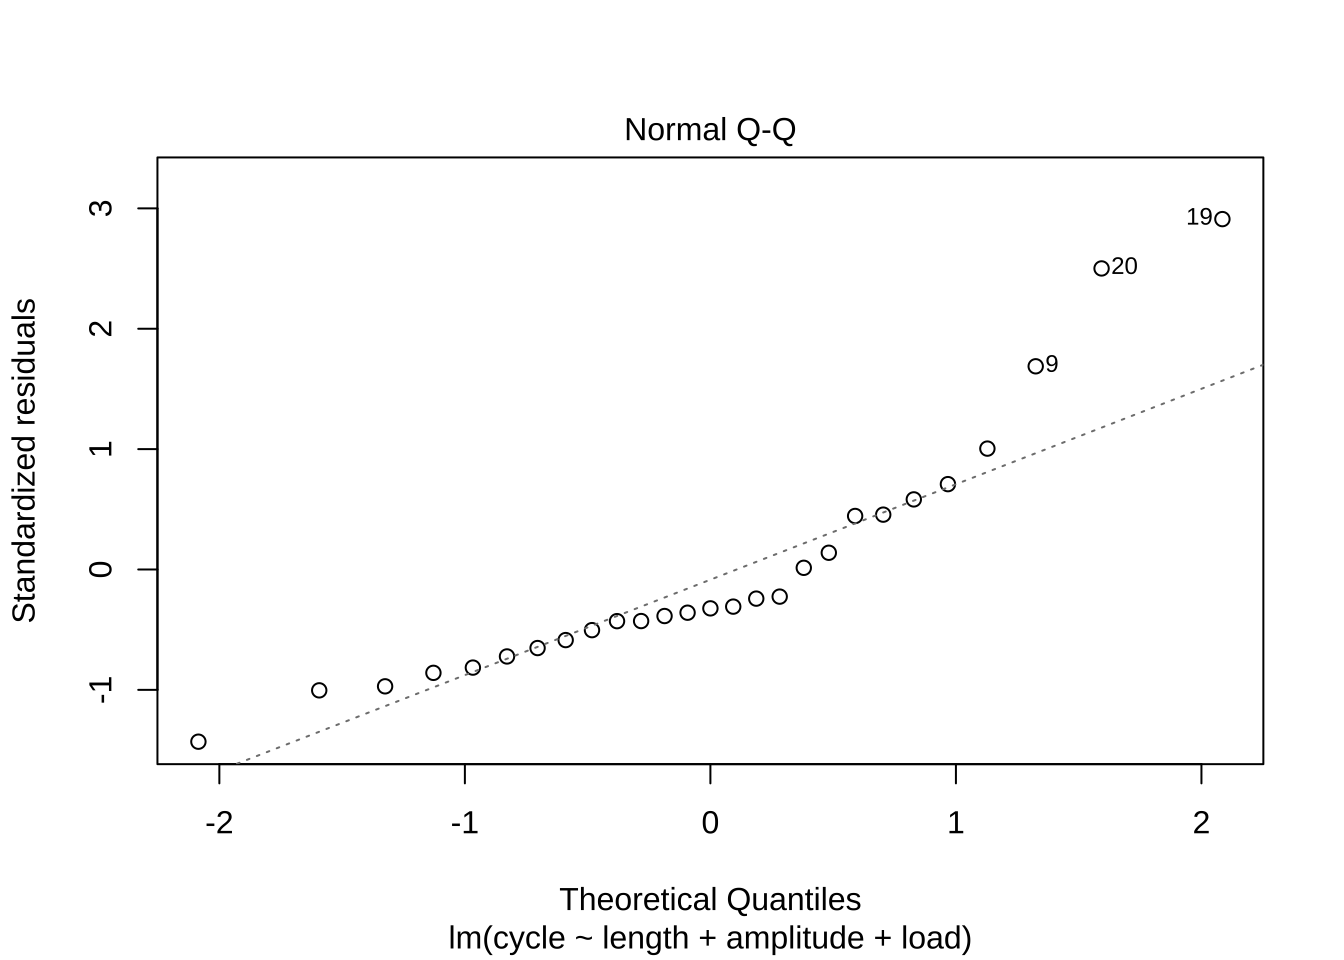
\includegraphics{lmpractice_files/figure-latex/unnamed-chunk-38-2.pdf} 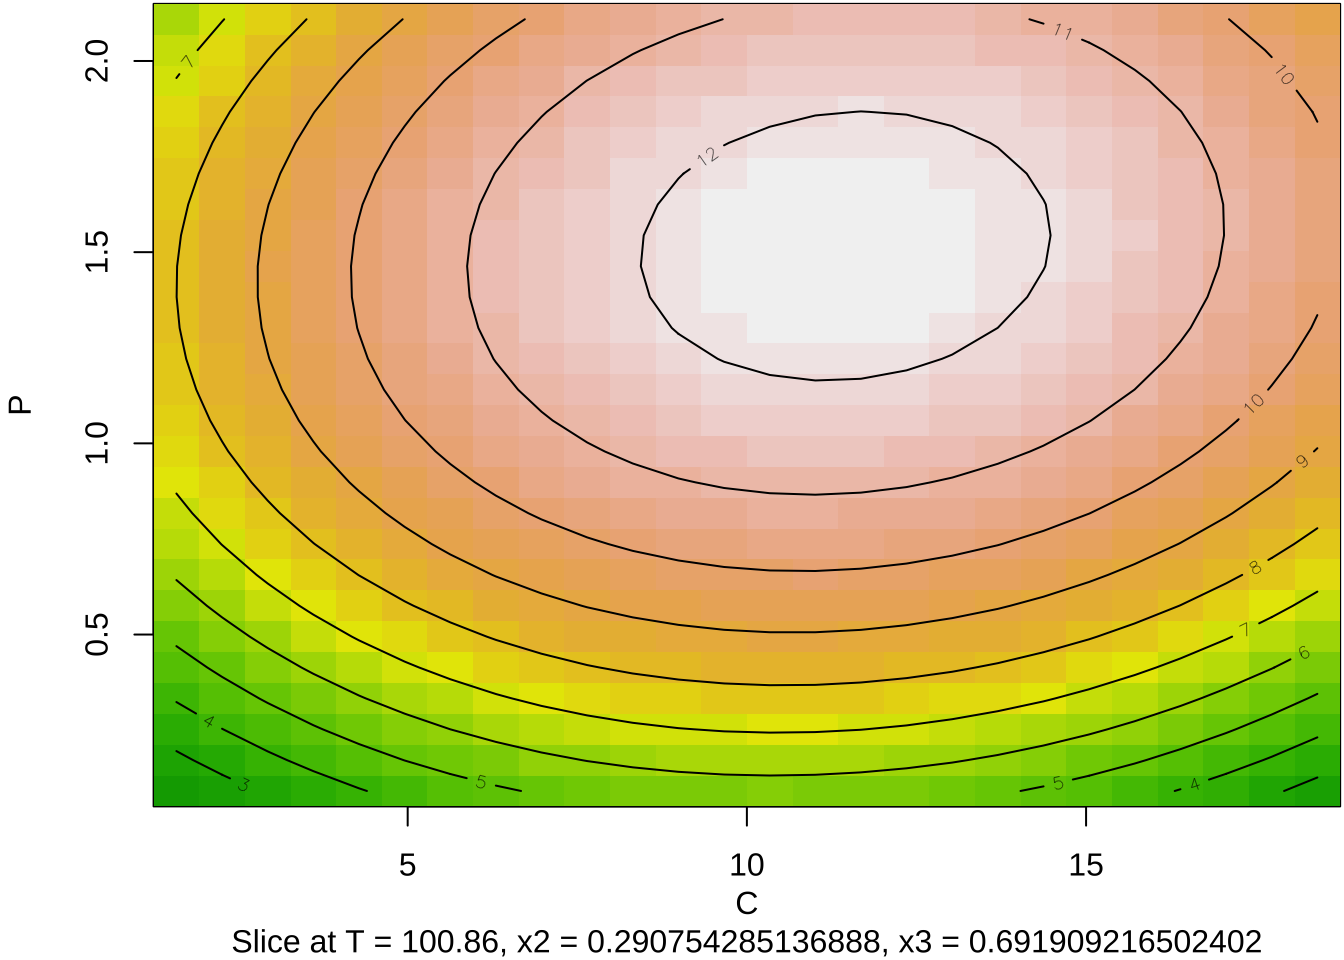
\includegraphics{lmpractice_files/figure-latex/unnamed-chunk-38-3.pdf} 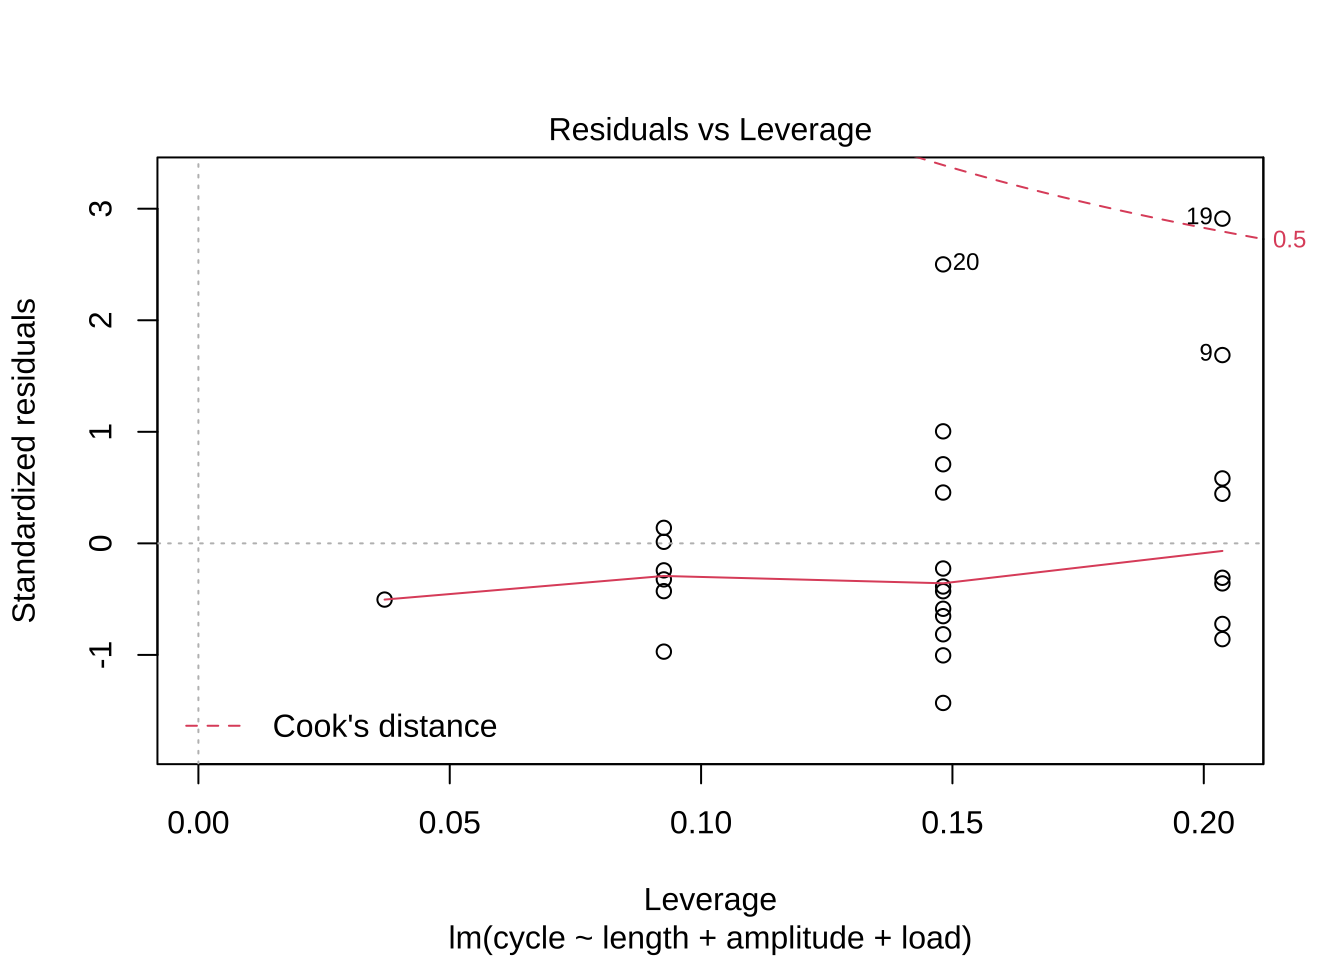
\includegraphics{lmpractice_files/figure-latex/unnamed-chunk-38-4.pdf}

\begin{Shaded}
\begin{Highlighting}[]
\NormalTok{wool}\SpecialCharTok{$}\NormalTok{logcycle }\OtherTok{\textless{}{-}} \FunctionTok{log}\NormalTok{(wool}\SpecialCharTok{$}\NormalTok{cycle)}
\FunctionTok{boxcox}\NormalTok{(woolfm1)}
\end{Highlighting}
\end{Shaded}

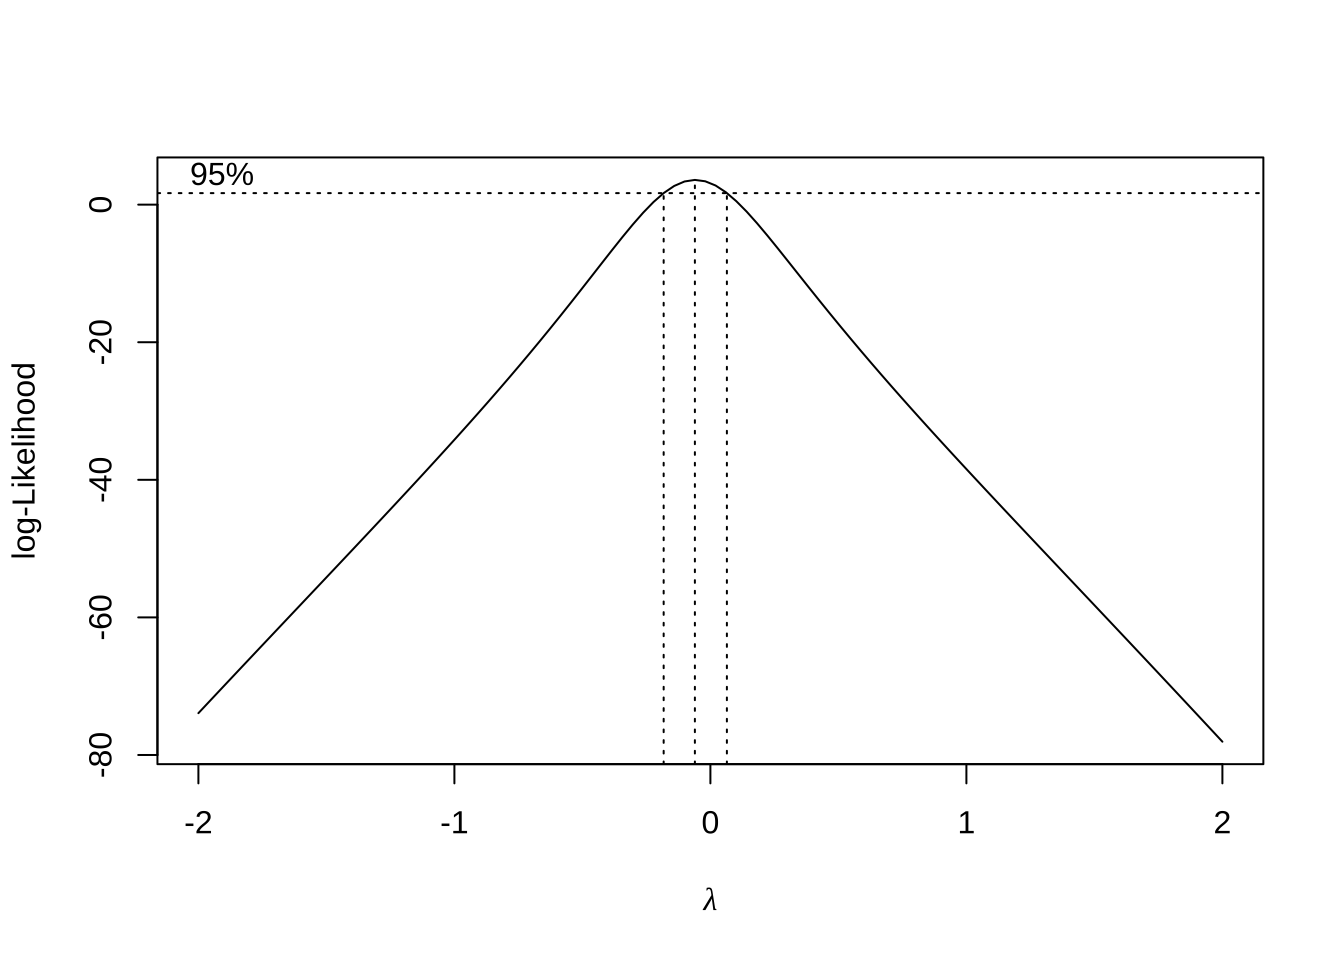
\includegraphics{lmpractice_files/figure-latex/unnamed-chunk-38-5.pdf}

\begin{Shaded}
\begin{Highlighting}[]
\NormalTok{woolfm2 }\OtherTok{\textless{}{-}} \FunctionTok{lm}\NormalTok{(logcycle}\SpecialCharTok{\textasciitilde{}}\NormalTok{length }\SpecialCharTok{+}\NormalTok{ amplitude }\SpecialCharTok{+}\NormalTok{ load, }\AttributeTok{data=}\NormalTok{wool)}
\FunctionTok{plot}\NormalTok{(woolfm2)}
\end{Highlighting}
\end{Shaded}

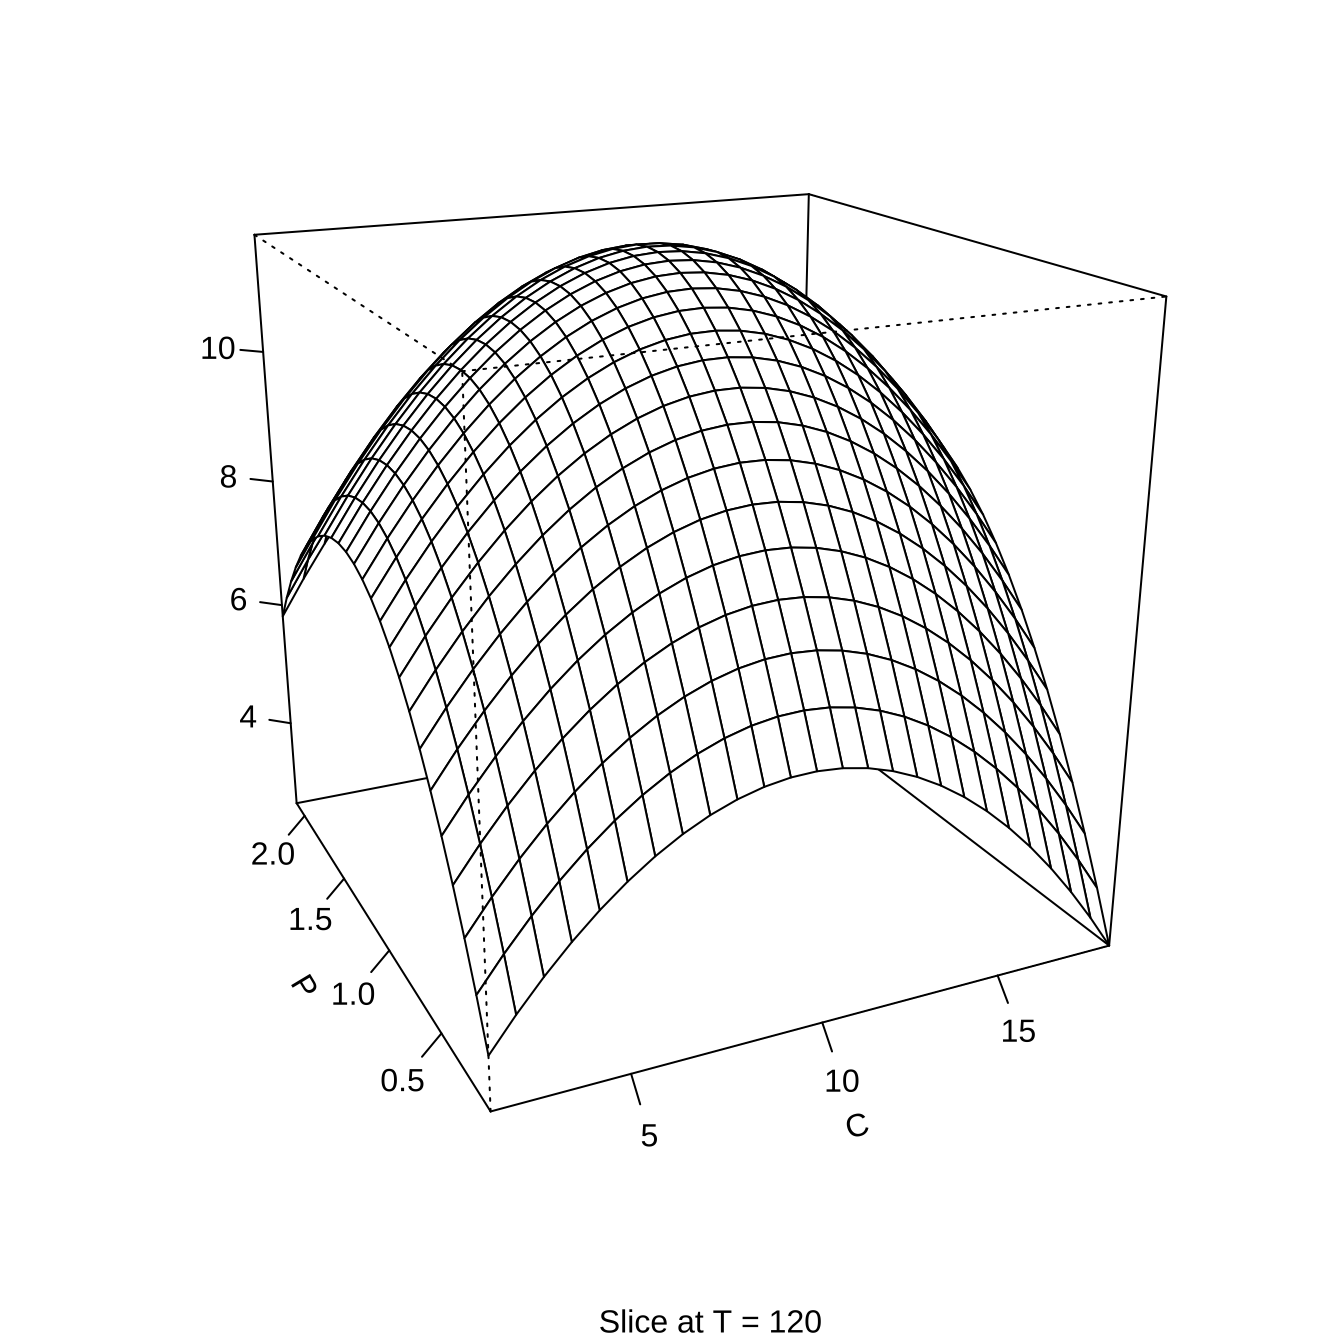
\includegraphics{lmpractice_files/figure-latex/unnamed-chunk-38-6.pdf} 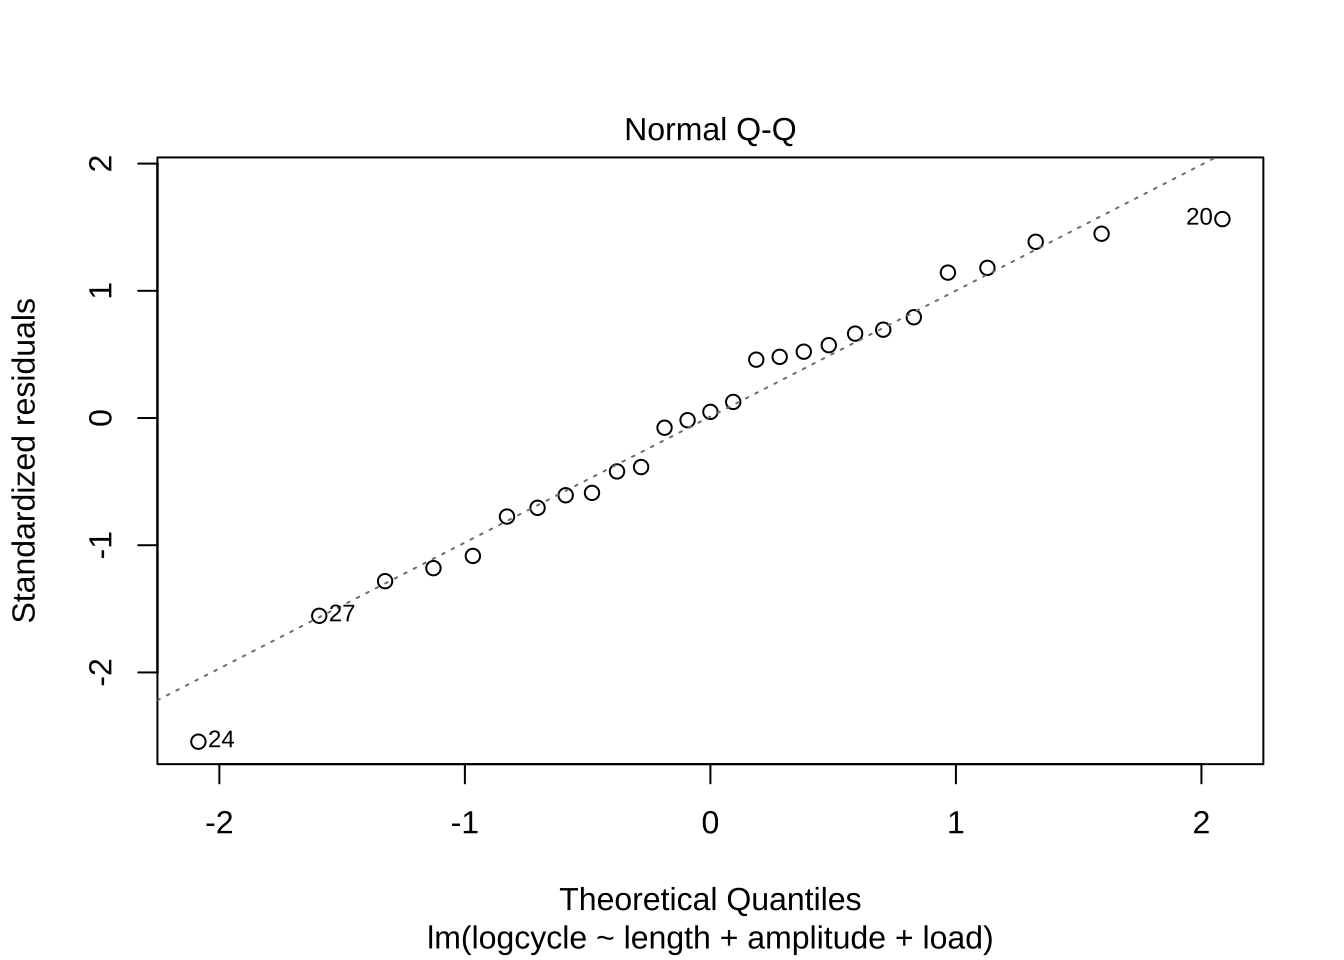
\includegraphics{lmpractice_files/figure-latex/unnamed-chunk-38-7.pdf} 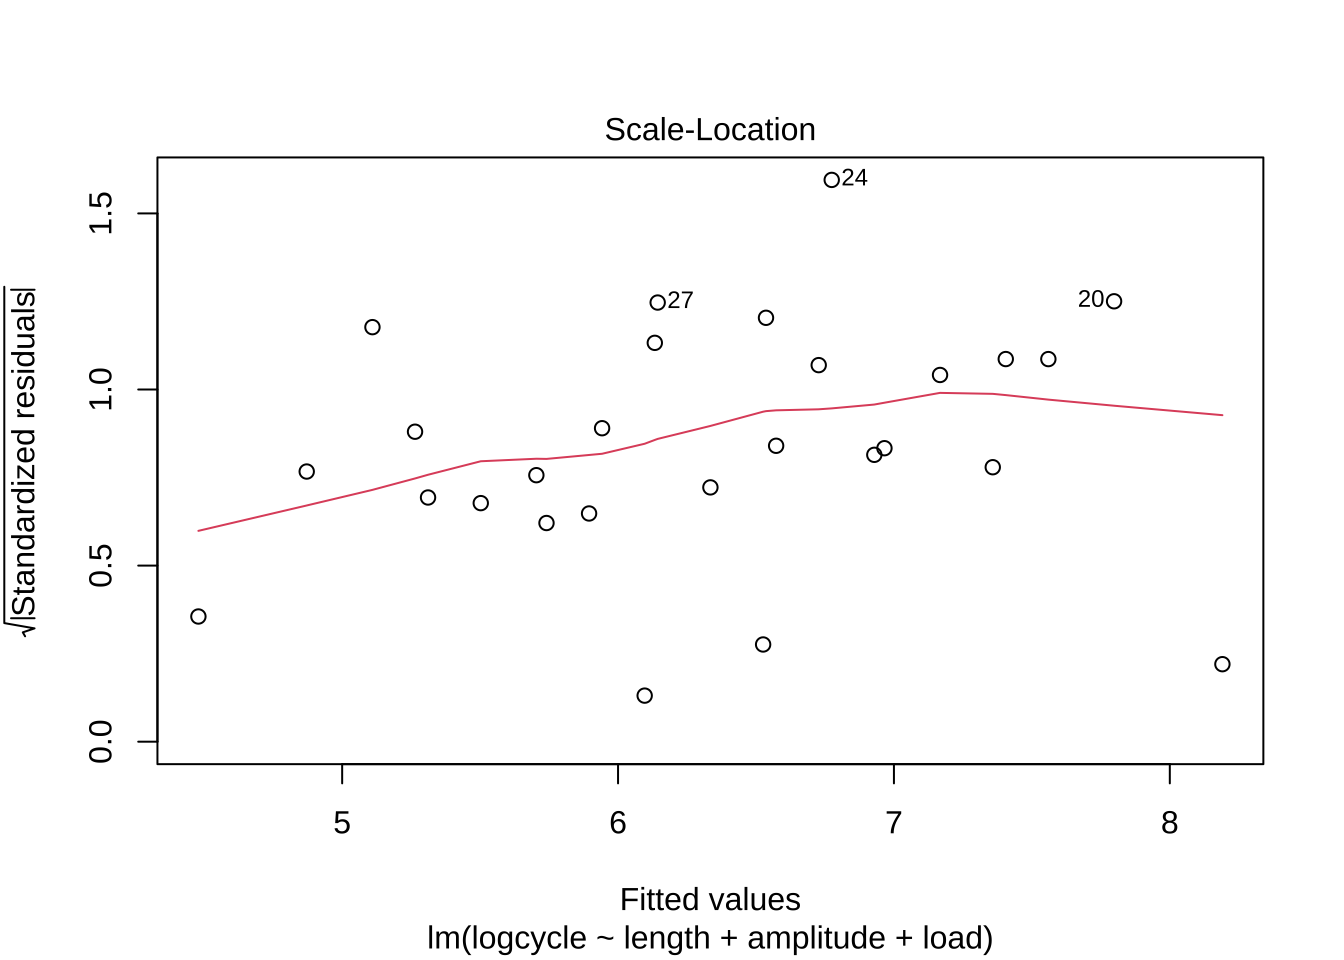
\includegraphics{lmpractice_files/figure-latex/unnamed-chunk-38-8.pdf} 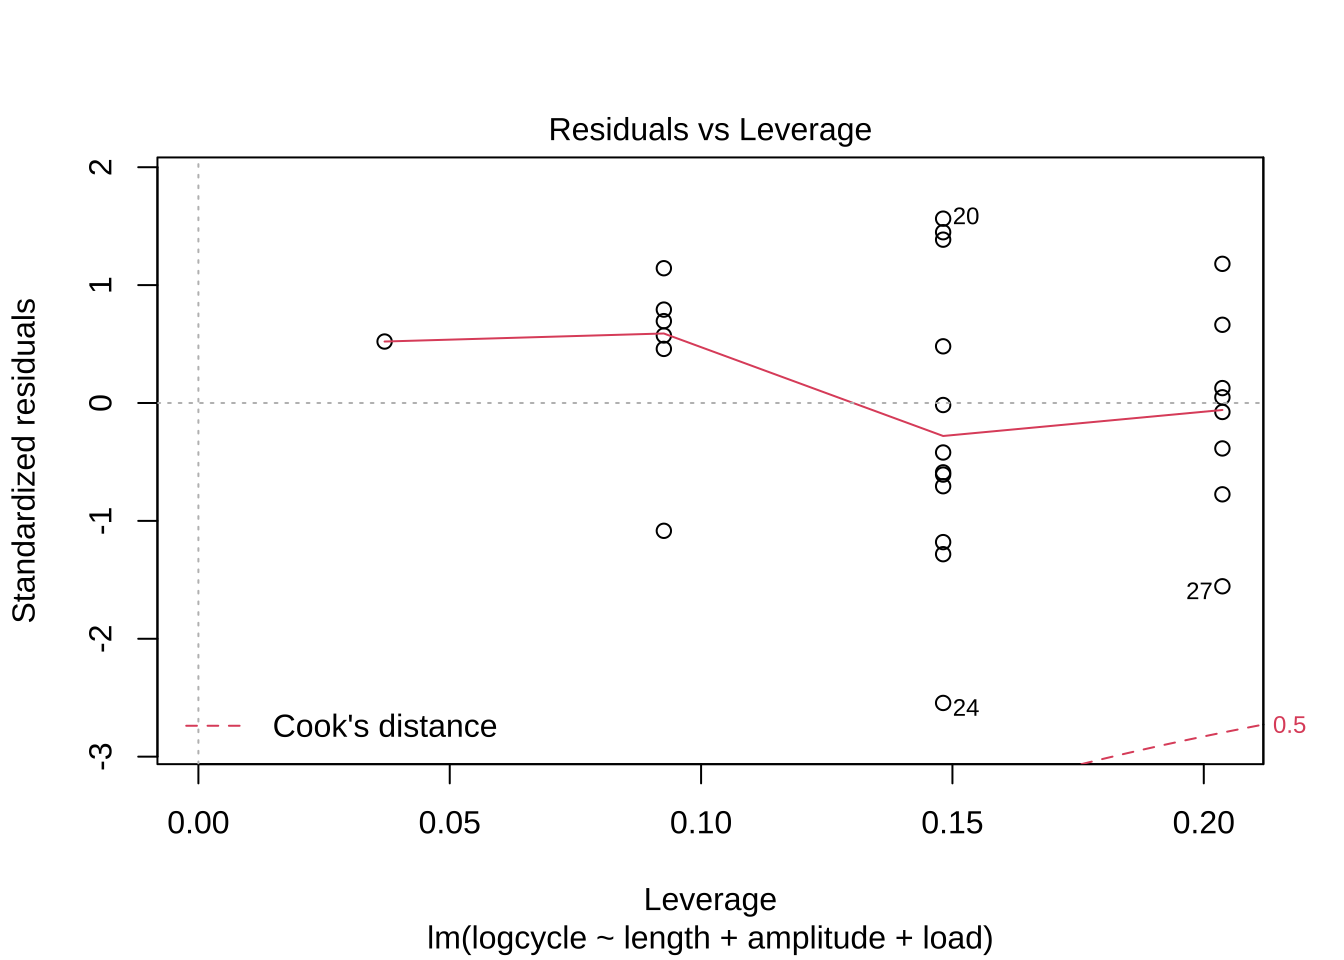
\includegraphics{lmpractice_files/figure-latex/unnamed-chunk-38-9.pdf}

\hypertarget{uxb2e4uxc911uxacf5uxc120uxc131}{%
\section{다중공선성}\label{uxb2e4uxc911uxacf5uxc120uxc131}}

\hypertarget{uxace0uxc720uxac12uxacfc-uxace0uxc720uxbca1uxd130uxc5d0-uxb300uxd55c-uxc774uxb860}{%
\subsection{고유값과 고유벡터에 대한 이론}\label{uxace0uxc720uxac12uxacfc-uxace0uxc720uxbca1uxd130uxc5d0-uxb300uxd55c-uxc774uxb860}}

대칭행렬 \(\bm A = \bm X^t\bm X\)의 고유값 \(\lambda_i\)와 그에 대응하는 고유벡터
\(\bm v_i\)는 다음을 만족하는 실수와 벡터이다.

\[ \bm A \bm  v_i = \lambda_i \bm  v_i \]

고유값 \(\lambda_i\)을 구하는 방법은 다음의 방정식을 만족하는 해를 구하는 것이다.

\[ det \left ( \bm A - \lambda_i \bm I \right ) = 0\]

여기서 \(det(\bm A)\)는 행렬 \(\bm A\)의 행렬식을 의미한다.

\(\lambda_1 \ge \lambda_2 \ge \dots \ge \lambda_{p-1}\)를 \(\bm X^t \bm X\)의 고유값이라고 하자. \(\bm X^t \bm X\)의 각 고유값에 대한 정규직교 고유벡터(orthonormal eigenvector)를 \(\bm v_1, \bm v_2,\dots,\bm v_{p-1}\)라고 하자, 즉

\[ \bm  v_i^t \bm  v_i = 1 , \quad \bm  v_i^t \bm  v_j = 0 \quad (i \ne j) \]

더 나아가 행렬 \(\bm V\)를 고유벡터를 모아놓은 행렬로 정의하자.

\[ \bm V=[\bm v_1 ~ \bm v_2 ~\dots ~ \bm v_{p-1} ] \]

이때 \((p-1) \times (p-1)\) 차원의 행렬 \(\bm V\)는 직교행렬이다.

\[ \bm V^t \bm V =\bm V  \bm V^t =I \]

이제 다음과 같이 \(\bm X^t \bm X\)를 나타낼 수 있다.

\[ \bm V^t (\bm X^t \bm X) \bm V = \text{diag}(\lambda_1 , \lambda_2 , \dots , \lambda_{p-1}) = \bm \Lambda \]

또한

\[ \bm V^t (\bm X^t \bm X)^{-1} \bm V = \text{diag} \left (\frac{1}{\lambda_1} , \frac{1}{\lambda_2} , \dots , \frac{1}{\lambda_{p-1}} \right ) = \bm \Lambda^{-1} \]

위의 식에서 알 수 있듯이 \(1/\lambda_i\)는 \((\bm X^t \bm X)^{-1}\)의 고유값이다.

행렬 \(\bm V\)가 직교행렬이기 때문에 다음과 같은 표현도 가능하다.

\[ (\bm X^t \bm X) =  \bm V \bm \Lambda \bm V^t, 
\quad (\bm X^t \bm X)^{-1} =  \bm V \bm \Lambda^{-1} \bm V^t  \]

따라서 고유값 \(\lambda_k\)이 매우 0에 가까우면 다음이 성립하고

\[ \bm v_k^t (\bm X^t \bm X) \bm v_k = (\bm X \bm v_k)^t ( \bm X \bm v_k) \approx 0   \]
위의 식은 다음과 같이 행렬 \(\bm X\)의 열들간에 선형관계가 있다는 것을 의미한다.

\[  v_{1k} \bm X_1 +  v_{2k} \bm X_2 + \dots  v_{p-1,k} \bm X_k \approx 0 \]

위에서 \(\bm v_k\)와 \(\bm X\)는 다음과 같이 표시한다.

\[ \bm X=[\bm X_1~ \bm X_2~ \dots~\bm X_{p-1}], \quad 
\bm v_k = [ v_{1k},  v_{2k}, \cdots,  v_{p-1,k}]^t \]

또한 회귀계수 벡터 \(\hat \beta\)의 공분산 행렬이 다음과 같이 주어지므로

\begin{equation} 
Cov(\hat {\bm \beta}) = \sigma^2 (\bm X^t \bm X)^{-1} = \sigma^2  \bm V \bm \Lambda^{-1} \bm V^t 
\label{eq:eq1}
\end{equation}

다음과 같은 식이 성립한다.

\begin{equation} 
var(\hat \beta_j) / \sigma^2 = \frac{v^2_{j1}}{\lambda_1} + \frac{v^2_{j2}}{\lambda_2} + \dots \frac{v^2_{j, p-1}}{\lambda_{p-1}} 
\label{eq:eq2}
\end{equation}

\hypertarget{uxace0uxc720uxac12uxacfc-uxace0uxc720uxbca1uxd130uxc5d0-uxb300uxd55c-uxc608uxc81c-uxb450-uxac1cuxc758-uxb3c5uxb9bduxbcc0uxc218}{%
\subsection{고유값과 고유벡터에 대한 예제: 두 개의 독립변수}\label{uxace0uxc720uxac12uxacfc-uxace0uxc720uxbca1uxd130uxc5d0-uxb300uxd55c-uxc608uxc81c-uxb450-uxac1cuxc758-uxb3c5uxb9bduxbcc0uxc218}}

이제 다음과 두 개의 독립변수가 있는 회귀 모형을 고려해 보자.

\[ y_i = \beta_0 + \beta_1 x_{i1} + \beta_2 x_{i2} + e_i, i=1,2,\cdots,n \]

절편을 제외한 두 개의 표준화된 독립변수들로 이루어진 행렬을 \(\bm X\)로 표시하자.

\[  \bm X = [ \bm X_1 ~ \bm X_2 ]   \]

위에서 디자인 행렬 \(\bm X\)는 원래 독립변수의 디자인 행렬 \(X\)의 열들을 표준화한 변수로 구성된 것이다..

이제 \(\bm X^t \bm X\)는 두 독립변수의 상관계수 행렬임을 알 수 있다.

\[  \bm X^t \bm X =
\begin{bmatrix}
1  &  \rho \\
\rho & 1 
\end{bmatrix} 
=\bm R, \quad
0 < \rho < 1
\]

여기서 두 독립변수 \(X_1\)과 \(X_2\)의 상관계수 \(\rho\)는 0보다 크다고 가정하자.

이제 \(\bm X^t \bm X\)의 고유값(\(\lambda_i\))과 고유벡터(\(\bm v_i\))는 다음과 같은 방정식을 만족하는 수 \(\lambda_i\)와 벡터 \(\bm v_i\) 이다.

\[ (\bm X^t \bm X) \bm v_i = \lambda_i \bm v_i, \quad \bm v_i^t \bm v_i=1  \]

일단 먼저 고유값을 구하는 방법은 \(det(\bm X^t \bm X - \lambda_i \bm I ) =0\)을 만족하는
값을 찾는 것이다. 여기서 \(det(\bm A)\)는 \(\bm A\)의 행렬식을 의미한다.

\[ 
det(\bm X^t \bm X - \lambda_i \bm I ) = det \left ( 
\begin{bmatrix}
1-\lambda_i  &  \rho \\
\rho & 1-\lambda_i 
\end{bmatrix}
 \right ) =0
\]
위의 방정식은 다음과 같이 요약할 수 있고

\[ \lambda_i^2 -2 \lambda_i + (1-\rho^2) =0 \]

해는 다음과 같이 주어진다.

\[ \lambda_1 = 1+ \rho, \quad \lambda_2 = 1 -\rho \quad (\lambda_1 \ge \lambda_2) \]

이제 각 고유값에 대한 고유벡터를 구해보자. 각 고유값 \(\lambda_i\)에 대한 고유벡터를 \(\bm v_i\) 라고 하면

\[ 
\bm v_1 = 
\begin{bmatrix} 
 v_{11} \\
 v_{21}
\end{bmatrix},
~ v^2_{11}+v^2_{21}=1
\quad \quad
\bm v_2 = 
\begin{bmatrix} 
 v_{12} \\
 v_{22}
\end{bmatrix},~
v^2_{12}+v^2_{11}=1
\]

다음과 같은 방정식을 만족해야 한다.

\[ (\bm X^t \bm X) \bm v_1 = \lambda_1 \bm v_1 , \quad  (\bm X^t \bm X) \bm v_2 = \lambda_2 \bm v_2 \]

즉,

\[ 
\begin{bmatrix}
1  &  \rho \\
\rho & 1 
\end{bmatrix}
\begin{bmatrix} 
 v_{11} \\
 v_{21}
\end{bmatrix}
=
(1+ \rho)
\begin{bmatrix} 
 v_{11} \\
 v_{21}
\end{bmatrix}
, \quad 
\begin{bmatrix}
1  &  \rho \\
\rho & 1 
\end{bmatrix}
\begin{bmatrix} 
 v_{12} \\
 v_{22}
\end{bmatrix}
=
(1- \rho)
\begin{bmatrix} 
 v_{12} \\
 v_{22}
\end{bmatrix}
\]

위의 두 방정식은 정리하면 다음과 더 단순한 방정식을 얻는다.

\[  v_{11} -  v_{21} = 0, \quad  v_{12}+ v_{22}=0 \]

이제 위의 식을 만족하고 길이가 1인 두 벡터를 찾으면 다음과 같은 두 개의 직교하고 길이가 1인 고유벡터 \(\bm v_1\)과 \(\bm v_2\)를 찾을 수 있다.

\[ 
\bm v_1 = 
\begin{bmatrix} 
 v_{11} \\
 v_{21}
\end{bmatrix}
= 
\begin{bmatrix} 
1/\sqrt{2} \\
1/\sqrt{2}
\end{bmatrix},
\quad \quad
\bm v_2 = 
\begin{bmatrix} 
 v_{12} \\
 v_{22}
\end{bmatrix}
= 
\begin{bmatrix} 
1/\sqrt{2} \\
-1/\sqrt{2}
\end{bmatrix}
\]

따라서 앞 절의 이론에서 나온 고유벡터로 구성된 행렬 \(\bm V\)와 고유값을 대각원소로 하는 행렬 \(\bm \Lambda\)는 다음과 같다.

\[ 
\bm V = [\bm v_1~ \bm v_2]
= \begin{bmatrix} 
 v_{11} &  v_{12}\\
 v_{21} &  v_{22}
\end{bmatrix}
= 
\begin{bmatrix} 
1/\sqrt{2} &  1/\sqrt{2}\\
1/\sqrt{2} &  -1/\sqrt{2}
\end{bmatrix},
\quad \quad
\bm \Lambda =
 \begin{bmatrix} 
\lambda_1 & 0 \\
0 & \lambda_2
\end{bmatrix}
= 
 \begin{bmatrix} 
1+\rho & 0 \\
0 & 1-\rho
\end{bmatrix}
\]

이제 다음이 성립함을 확인할 수 있다.

\[ \bm V^t (\bm X^t \bm X) \bm V =  \bm \Lambda, \quad (\bm X^t \bm X)^{-1} =  \bm V \bm \Lambda^{-1} \bm V^t   \]

즉,

\begin{align*}
\bm V^t (\bm X^t \bm X) \bm V 
& =  
\begin{bmatrix} 
1/\sqrt{2} &  1/\sqrt{2}\\
1/\sqrt{2} &  -1/\sqrt{2}
\end{bmatrix}
\begin{bmatrix} 
1 & \rho \\
\rho & 1
\end{bmatrix}
\begin{bmatrix} 
1/\sqrt{2} &  1/\sqrt{2}\\
1/\sqrt{2} &  -1/\sqrt{2}
\end{bmatrix} \\
& =
 \begin{bmatrix} 
1+\rho & 0 \\
0 & 1-\rho
\end{bmatrix} \\
&=
\bm \Lambda
\end{align*}

또한 다음도 성립함을 확인할 수 있다.

\[  (\bm X^t \bm X)^{-1} =  \bm V \bm \Lambda^{-1} \bm V^t   \]

즉,

\begin{align*}
(\bm X^t \bm X)^{-1} & =  \bm V \bm \Lambda^{-1} \bm V^t \\   
 &  = 
 \begin{bmatrix} 
 v_{11} &  v_{12}\\
 v_{21} &  v_{22}
\end{bmatrix}
 \begin{bmatrix} 
\frac{1}{\lambda_1} & 0 \\
0 & \frac{1}{\lambda_2}
\end{bmatrix} 
\begin{bmatrix} 
 v_{11} &  v_{21}\\
 v_{12} &  v_{22}
\end{bmatrix} \\
&= 
\begin{bmatrix} 
1/\sqrt{2} &  1/\sqrt{2}\\
1/\sqrt{2} &  -1/\sqrt{2}
\end{bmatrix}
 \begin{bmatrix} 
\frac{1}{1+\rho} & 0 \\
0 & \frac{1}{1-\rho}
\end{bmatrix}
\begin{bmatrix} 
1/\sqrt{2} &  1/\sqrt{2}\\
1/\sqrt{2} &  -1/\sqrt{2}
\end{bmatrix} \\
&=
 \begin{bmatrix} 
 v_{11}^2 \frac{1}{\lambda_1} +   v_{12}^2 \frac{1}{\lambda_2} &
 v_{11}  v_{21} \frac{1}{\lambda_1} +  v_{12}  v_{22} \frac{1}{\lambda_2} \\
 v_{11}  v_{21} \frac{1}{\lambda_1} +  v_{12}  v_{22} \frac{1}{\lambda_2}   & 
 v_{21}^2 \frac{1}{\lambda_1} +   v_{22}^2 \frac{1}{\lambda_2}
\end{bmatrix} \\
&= 
\begin{bmatrix} 
(\frac{1}{\sqrt{2}})^2 \frac{1}{1+\rho} +  (\frac{1}{\sqrt{2}})^2 \frac{1}{1-\rho} &
(\frac{1}{\sqrt{2}})^2 \frac{1}{1+\rho} + (\frac{1}{\sqrt{2}}) (-\frac{1}{\sqrt{2}}) \frac{1}{1-\rho} \\
(\frac{1}{\sqrt{2}})^2 \frac{1}{1+\rho} + (\frac{1}{\sqrt{2}}) (-\frac{1}{\sqrt{2}}) \frac{1}{1-\rho}  & 
(\frac{1}{\sqrt{2}})^2 \frac{1}{1+\rho} +  (-\frac{1}{\sqrt{2}})^2 \frac{1}{1-\rho} 
\end{bmatrix} \\
& =
\frac{1}{1-\rho^2}
\begin{bmatrix}
1  & -\rho \\
-\rho & 1
\end{bmatrix}
\end{align*}

앞 절에서 나온 회귀계수 추정량의 분산 공식 \eqref{eq:eq1} 과 \eqref{eq:eq2} 를 적용하면 다음과 같은 식을 얻을 수 있다.

\begin{align*}
Var(\hat \beta_j)/\sigma^2 
& = \frac{v^2_{j1}}{\lambda_1} + \frac{v^2_{j2}}{\lambda_2} \\
& = \frac{1}{2} \left ( \frac{1}{1+\rho} + \frac{1}{1-\rho} \right ) \\
& = \frac{1}{1-\rho^2}
\end{align*}

위의 분산 공식에서 제일 작은 두 번째 고유값 \(\lambda_2 = 1- \rho\)가 0에 가까우면 분산이 매우 커지는 것을 알 수 있다. 이 고유값은 상관계수 \(\rho\)가 1에 가까울 수록 0에 가까워 진다.

\hypertarget{uxc911uxace0uxcc28-uxc608uxc81c}{%
\subsection{중고차 예제}\label{uxc911uxace0uxcc28-uxc608uxc81c}}

\begin{Shaded}
\begin{Highlighting}[]
\NormalTok{usedcars2 }\OtherTok{\textless{}{-}}\NormalTok{ usedcars }\SpecialCharTok{\%\textgreater{}\%}  \FunctionTok{mutate}\NormalTok{(}\AttributeTok{ccmile =}\NormalTok{ cc }\SpecialCharTok{+}\NormalTok{ mileage)}
\NormalTok{fitcoll1 }\OtherTok{\textless{}{-}} \FunctionTok{lm}\NormalTok{(price }\SpecialCharTok{\textasciitilde{}}\NormalTok{ year }\SpecialCharTok{+}\NormalTok{ mileage }\SpecialCharTok{+}\NormalTok{ cc }\SpecialCharTok{+}\NormalTok{ automatic }\SpecialCharTok{+}\NormalTok{ ccmile, usedcars2)}
\FunctionTok{summary}\NormalTok{(fitcoll1)}
\end{Highlighting}
\end{Shaded}

\begin{verbatim}
## 
## Call:
## lm(formula = price ~ year + mileage + cc + automatic + ccmile, 
##     data = usedcars2)
## 
## Residuals:
##     Min      1Q  Median      3Q     Max 
## -177.35  -63.91   -0.99   70.34  212.69 
## 
## Coefficients: (1 not defined because of singularities)
##               Estimate Std. Error t value Pr(>|t|)    
## (Intercept)  5.253e+02  3.998e+02   1.314 0.200823    
## year        -5.800e+00  9.283e-01  -6.247 1.55e-06 ***
## mileage     -2.263e-03  7.211e-04  -3.138 0.004324 ** 
## cc           3.888e-01  2.022e-01   1.923 0.065958 .  
## automatic    1.653e+02  3.986e+01   4.147 0.000339 ***
## ccmile              NA         NA      NA       NA    
## ---
## Signif. codes:  0 '***' 0.001 '**' 0.01 '*' 0.05 '.' 0.1 ' ' 1
## 
## Residual standard error: 101.1 on 25 degrees of freedom
## Multiple R-squared:  0.9045, Adjusted R-squared:  0.8892 
## F-statistic: 59.21 on 4 and 25 DF,  p-value: 2.184e-12
\end{verbatim}

\hypertarget{uxc608uxc81c-4.14}{%
\subsection{예제 4.14}\label{uxc608uxc81c-4.14}}

모형을 적합해 보자.

\begin{Shaded}
\begin{Highlighting}[]
\NormalTok{hald.lm }\OtherTok{\textless{}{-}} \FunctionTok{lm}\NormalTok{(y}\SpecialCharTok{\textasciitilde{}}\NormalTok{ ., }\AttributeTok{data=}\NormalTok{hald)}
\FunctionTok{summary}\NormalTok{(hald.lm)}
\end{Highlighting}
\end{Shaded}

\begin{verbatim}
## 
## Call:
## lm(formula = y ~ ., data = hald)
## 
## Residuals:
##     Min      1Q  Median      3Q     Max 
## -3.1750 -1.6709  0.2508  1.3783  3.9254 
## 
## Coefficients:
##             Estimate Std. Error t value Pr(>|t|)  
## (Intercept)  62.4054    70.0710   0.891   0.3991  
## x1            1.5511     0.7448   2.083   0.0708 .
## x2            0.5102     0.7238   0.705   0.5009  
## x3            0.1019     0.7547   0.135   0.8959  
## x4           -0.1441     0.7091  -0.203   0.8441  
## ---
## Signif. codes:  0 '***' 0.001 '**' 0.01 '*' 0.05 '.' 0.1 ' ' 1
## 
## Residual standard error: 2.446 on 8 degrees of freedom
## Multiple R-squared:  0.9824, Adjusted R-squared:  0.9736 
## F-statistic: 111.5 on 4 and 8 DF,  p-value: 4.756e-07
\end{verbatim}

상관계수 행렬의 고유값을 계산해 보자.

\begin{Shaded}
\begin{Highlighting}[]
\NormalTok{R }\OtherTok{\textless{}{-}} \FunctionTok{cor}\NormalTok{(hald[}\DecValTok{2}\SpecialCharTok{:}\DecValTok{5}\NormalTok{])}
\NormalTok{R}
\end{Highlighting}
\end{Shaded}

\begin{verbatim}
##            x1         x2         x3         x4
## x1  1.0000000  0.2285795 -0.8241338 -0.2454451
## x2  0.2285795  1.0000000 -0.1392424 -0.9729550
## x3 -0.8241338 -0.1392424  1.0000000  0.0295370
## x4 -0.2454451 -0.9729550  0.0295370  1.0000000
\end{verbatim}

\begin{Shaded}
\begin{Highlighting}[]
\FunctionTok{solve}\NormalTok{(R)}
\end{Highlighting}
\end{Shaded}

\begin{verbatim}
##          x1        x2        x3       x4
## x1 38.49621  94.11969  41.88410  99.7858
## x2 94.11969 254.42317 105.09139 267.5394
## x3 41.88410 105.09139  46.86839 111.1451
## x4 99.78580 267.53942 111.14509 282.5129
\end{verbatim}

\begin{Shaded}
\begin{Highlighting}[]
\FunctionTok{diag}\NormalTok{(}\FunctionTok{solve}\NormalTok{(R))}
\end{Highlighting}
\end{Shaded}

\begin{verbatim}
##        x1        x2        x3        x4 
##  38.49621 254.42317  46.86839 282.51286
\end{verbatim}

\begin{Shaded}
\begin{Highlighting}[]
\NormalTok{eigenval }\OtherTok{\textless{}{-}} \FunctionTok{eigen}\NormalTok{(R)}\SpecialCharTok{$}\NormalTok{values}
\NormalTok{eigenval}
\end{Highlighting}
\end{Shaded}

\begin{verbatim}
## [1] 2.235704035 1.576066070 0.186606149 0.001623746
\end{verbatim}

\begin{Shaded}
\begin{Highlighting}[]
\FunctionTok{sqrt}\NormalTok{(}\FunctionTok{max}\NormalTok{(eigenval)}\SpecialCharTok{/}\NormalTok{eigenval)}
\end{Highlighting}
\end{Shaded}

\begin{verbatim}
## [1]  1.000000  1.191022  3.461339 37.106342
\end{verbatim}

VIF를 구해보자.

\begin{Shaded}
\begin{Highlighting}[]
\NormalTok{car}\SpecialCharTok{::}\FunctionTok{vif}\NormalTok{(hald.lm)}
\end{Highlighting}
\end{Shaded}

\begin{verbatim}
##        x1        x2        x3        x4 
##  38.49621 254.42317  46.86839 282.51286
\end{verbatim}

\begin{Shaded}
\begin{Highlighting}[]
\FunctionTok{summary}\NormalTok{(regbook}\SpecialCharTok{::}\FunctionTok{vif}\NormalTok{(hald.lm))}
\end{Highlighting}
\end{Shaded}

\begin{verbatim}
## 
## VIF:
##     x1     x2     x3     x4 
##  38.50 254.42  46.87 282.51 
## 
## Variance Proportion:
##   Eigenvalues Cond.Index          x1           x2          x3           x4
## 1 2.235704035   1.000000 0.002632084 0.0005589686 0.001481988 0.0004753347
## 2 1.576066070   1.191022 0.004269804 0.0004272931 0.004954638 0.0004572915
## 3 0.186606149   3.461339 0.063519491 0.0020822791 0.046495910 0.0007243995
## 4 0.001623746  37.106342 0.929578621 0.9969314592 0.947067464 0.9983429744
\end{verbatim}

\(x_2\)를 제외하고 분석해 보자.

\begin{Shaded}
\begin{Highlighting}[]
\NormalTok{hald.lm2 }\OtherTok{\textless{}{-}} \FunctionTok{lm}\NormalTok{(y}\SpecialCharTok{\textasciitilde{}}\NormalTok{ x1 }\SpecialCharTok{+}\NormalTok{ x3 }\SpecialCharTok{+}\NormalTok{ x4, }\AttributeTok{data=}\NormalTok{hald)}
\FunctionTok{summary}\NormalTok{(hald.lm2)}
\end{Highlighting}
\end{Shaded}

\begin{verbatim}
## 
## Call:
## lm(formula = y ~ x1 + x3 + x4, data = hald)
## 
## Residuals:
##     Min      1Q  Median      3Q     Max 
## -2.9323 -1.8090  0.4806  1.1398  3.7771 
## 
## Coefficients:
##              Estimate Std. Error t value Pr(>|t|)    
## (Intercept) 111.68441    4.56248  24.479 1.52e-09 ***
## x1            1.05185    0.22368   4.702  0.00112 ** 
## x3           -0.41004    0.19923  -2.058  0.06969 .  
## x4           -0.64280    0.04454 -14.431 1.58e-07 ***
## ---
## Signif. codes:  0 '***' 0.001 '**' 0.01 '*' 0.05 '.' 0.1 ' ' 1
## 
## Residual standard error: 2.377 on 9 degrees of freedom
## Multiple R-squared:  0.9813, Adjusted R-squared:  0.975 
## F-statistic: 157.3 on 3 and 9 DF,  p-value: 4.312e-08
\end{verbatim}

\begin{Shaded}
\begin{Highlighting}[]
\FunctionTok{summary}\NormalTok{(regbook}\SpecialCharTok{::}\FunctionTok{vif}\NormalTok{(hald.lm2))}
\end{Highlighting}
\end{Shaded}

\begin{verbatim}
## 
## VIF:
##    x1    x3    x4 
## 3.678 3.460 1.181 
## 
## Variance Proportion:
##   Eigenvalues Cond.Index           x1         x3         x4
## 1   1.8683737   1.000000 0.0720157120 0.07053018 0.02229687
## 2   0.9838532   1.378056 0.0002285765 0.02382939 0.79011946
## 3   0.1477731   3.555775 0.9277557115 0.90564042 0.18758367
\end{verbatim}

\hypertarget{compute}{%
\chapter{최소제곱의 계산법}\label{compute}}

이제 선형모형에서 회귀게수를 구하는 계산 방법에 대하여 알아보자. 최소제곱법(동시에 최대 가능도 추정법)에 의한 회귀게수의 추정치를 구하려면 다음과 같은 정규 방정식(normal equation)을 풀어야 한다.

\begin{equation}
 {\bm X}^t \bm X \bm \beta = \bm X^t \bm y
\label{eq:comp-lse}
\end{equation}

중고차 자료를 이용한다.

\begin{Shaded}
\begin{Highlighting}[]
\FunctionTok{head}\NormalTok{(usedcars)}
\end{Highlighting}
\end{Shaded}

\begin{verbatim}
##   price year mileage   cc automatic
## 1   790   78  133462 1998         1
## 2  1380   39   33000 2000         1
## 3   270  109  120000 1800         0
## 4  1190   20   69727 1999         1
## 5   590   70  112000 2000         0
## 6  1120   58   39106 1998         1
\end{verbatim}

\begin{Shaded}
\begin{Highlighting}[]
\NormalTok{fit0 }\OtherTok{\textless{}{-}} \FunctionTok{lm}\NormalTok{(price }\SpecialCharTok{\textasciitilde{}}\NormalTok{ year }\SpecialCharTok{+}\NormalTok{ mileage }\SpecialCharTok{+}\NormalTok{ cc }\SpecialCharTok{+}\NormalTok{ automatic, }\AttributeTok{data=}\NormalTok{usedcars)}
\NormalTok{lmbeta }\OtherTok{\textless{}{-}}\NormalTok{ fit0}\SpecialCharTok{$}\NormalTok{coefficients}
\NormalTok{lmbeta}
\end{Highlighting}
\end{Shaded}

\begin{verbatim}
##   (Intercept)          year       mileage            cc     automatic 
## 525.286960604  -5.799637101  -0.002262844   0.388787346 165.312632517
\end{verbatim}

계획행렬은 다음과 같이 구할 수 있다.

\begin{Shaded}
\begin{Highlighting}[]
\NormalTok{X }\OtherTok{\textless{}{-}} \FunctionTok{model.matrix}\NormalTok{(fit0)}
\NormalTok{y }\OtherTok{\textless{}{-}} \FunctionTok{as.matrix}\NormalTok{(usedcars}\SpecialCharTok{$}\NormalTok{price)}
\NormalTok{X}
\end{Highlighting}
\end{Shaded}

\begin{verbatim}
##    (Intercept) year mileage   cc automatic
## 1            1   78  133462 1998         1
## 2            1   39   33000 2000         1
## 3            1  109  120000 1800         0
## 4            1   20   69727 1999         1
## 5            1   70  112000 2000         0
## 6            1   58   39106 1998         1
## 7            1   53   95935 1800         1
## 8            1   68  120000 1800         0
## 9            1   15   20215 1798         1
## 10           1   96  140000 1800         0
## 11           1   63   68924 1998         1
## 12           1   82   90000 2000         0
## 13           1   76   81279 1998         0
## 14           1   17   24070 1798         1
## 15           1   38   40000 2000         0
## 16           1   46   56887 1832         1
## 17           1   95   91216 1997         1
## 18           1   37   48680 1998         1
## 19           1   68    8000 2000         0
## 20           1   41   60634 1835         1
## 21           1   69  114131 1998         1
## 22           1   71   75000 1800         0
## 23           1   99  124417 1998         1
## 24           1  129  130000 1800         0
## 25           1   57   77559 1997         1
## 26           1  107   75216 1838         1
## 27           1   45   52000 2000         0
## 28           1   80   58000 2000         1
## 29           1  113  134500 1800         0
## 30           1   41   80000 2000         0
## attr(,"assign")
## [1] 0 1 2 3 4
\end{verbatim}

\begin{Shaded}
\begin{Highlighting}[]
\NormalTok{y}
\end{Highlighting}
\end{Shaded}

\begin{verbatim}
##       [,1]
##  [1,]  790
##  [2,] 1380
##  [3,]  270
##  [4,] 1190
##  [5,]  590
##  [6,] 1120
##  [7,]  815
##  [8,]  450
##  [9,] 1290
## [10,]  420
## [11,]  945
## [12,]  770
## [13,]  610
## [14,] 1350
## [15,] 1020
## [16,]  830
## [17,]  670
## [18,]  990
## [19,]  800
## [20,] 1100
## [21,]  740
## [22,]  570
## [23,]  660
## [24,]  300
## [25,]  960
## [26,]  650
## [27,] 1000
## [28,]  700
## [29,]  280
## [30,]  879
\end{verbatim}

\begin{Shaded}
\begin{Highlighting}[]
\NormalTok{A }\OtherTok{\textless{}{-}} \FunctionTok{t}\NormalTok{(X) }\SpecialCharTok{\%*\%}\NormalTok{ X}
\NormalTok{Xty }\OtherTok{\textless{}{-}} \FunctionTok{t}\NormalTok{(X) }\SpecialCharTok{\%*\%}\NormalTok{ y }
\NormalTok{A}
\end{Highlighting}
\end{Shaded}

\begin{verbatim}
##             (Intercept)      year      mileage         cc automatic
## (Intercept)          30      1980      2373958      57680        17
## year               1980    155858    179424383    3792473       974
## mileage         2373958 179424383 228412852144 4542340762   1191179
## cc                57680   3792473   4542340762  111163348     32882
## automatic            17       974      1191179      32882        17
\end{verbatim}

\begin{Shaded}
\begin{Highlighting}[]
\NormalTok{Xty}
\end{Highlighting}
\end{Shaded}

\begin{verbatim}
##                   [,1]
## (Intercept)      24139
## year           1365619
## mileage     1652471805
## cc            46679690
## automatic        16180
\end{verbatim}

\hypertarget{uxcd10uxb808uxc2a4uxd0a4}{%
\section{촐레스키}\label{uxcd10uxb808uxc2a4uxd0a4}}

\begin{Shaded}
\begin{Highlighting}[]
\NormalTok{U }\OtherTok{\textless{}{-}} \FunctionTok{chol}\NormalTok{(A) }\CommentTok{\# chol give upper diagonal}
\NormalTok{U}
\end{Highlighting}
\end{Shaded}

\begin{verbatim}
##             (Intercept)     year  mileage          cc  automatic
## (Intercept)    5.477226 361.4969 433423.4 10530.87904  3.1037612
## year           0.000000 158.6758 143331.0   -90.79521 -0.9327196
## mileage        0.000000   0.0000 141468.0   -63.44464 -0.1440343
## cc             0.000000   0.0000      0.0   501.66291  0.2050022
## automatic      0.000000   0.0000      0.0     0.00000  2.5365191
\end{verbatim}

\begin{Shaded}
\begin{Highlighting}[]
\NormalTok{bstar }\OtherTok{\textless{}{-}} \FunctionTok{solve}\NormalTok{(}\FunctionTok{t}\NormalTok{(U) ,Xty)}
\NormalTok{hatb\_chol }\OtherTok{\textless{}{-}} \FunctionTok{solve}\NormalTok{(U, bstar)}
\NormalTok{hatb\_chol}
\end{Highlighting}
\end{Shaded}

\begin{verbatim}
##                      [,1]
## (Intercept) 525.286960604
## year         -5.799637101
## mileage      -0.002262844
## cc            0.388787346
## automatic   165.312632517
\end{verbatim}

\hypertarget{qr}{%
\section{QR}\label{qr}}

\begin{Shaded}
\begin{Highlighting}[]
\NormalTok{QRans }\OtherTok{\textless{}{-}} \FunctionTok{qr}\NormalTok{(X)}
\NormalTok{Q1 }\OtherTok{\textless{}{-}} \FunctionTok{qr.Q}\NormalTok{(QRans)}
\NormalTok{Q1}
\end{Highlighting}
\end{Shaded}

\begin{verbatim}
##             [,1]        [,2]        [,3]       [,4]        [,5]
##  [1,] -0.1825742  0.07562591  0.30742310 -0.2027340  0.19971845
##  [2,] -0.1825742 -0.17015830 -0.15369537 -0.1039196  0.09114151
##  [3,] -0.1825742  0.27099286  0.01432404  0.1936620 -0.10728957
##  [4,] -0.1825742 -0.28989933  0.22723602 -0.1284304  0.06676071
##  [5,] -0.1825742  0.02520864  0.20679510 -0.1848696 -0.21733215
##  [6,] -0.1825742 -0.05041728 -0.23185156 -0.1117203  0.13010376
##  [7,] -0.1825742 -0.08192807  0.20178344  0.2338289  0.17106774
##  [8,] -0.1825742  0.01260432  0.27611529  0.2073189 -0.18633389
##  [9,] -0.1825742 -0.32141013 -0.09082550  0.3181650  0.07320675
## [10,] -0.1825742  0.18906478  0.23870575  0.1801128 -0.12576957
## [11,] -0.1825742 -0.01890648 -0.05300173 -0.1400423  0.14955765
## [12,] -0.1825742  0.10083455 -0.02533894 -0.1691993 -0.20143834
## [13,] -0.1825742  0.06302159 -0.04867448 -0.1554176 -0.21555404
## [14,] -0.1825742 -0.30880581 -0.07634583  0.3140525  0.07833142
## [15,] -0.1825742 -0.17646046 -0.09782906 -0.1098444 -0.30272348
## [16,] -0.1825742 -0.12604319 -0.02954052  0.2072806  0.13956469
## [17,] -0.1825742  0.18276262 -0.09975034 -0.1686365  0.21874911
## [18,] -0.1825742 -0.18276262 -0.03008727 -0.1132842  0.09276884
## [19,] -0.1825742  0.01260432 -0.51558321 -0.0912301 -0.25541870
## [20,] -0.1825742 -0.15755399  0.02887180  0.1996162  0.13067512
## [21,] -0.1825742  0.01890648  0.22824373 -0.1824548  0.17600462
## [22,] -0.1825742  0.03151080 -0.06113331  0.2465485 -0.19536153
## [23,] -0.1825742  0.20797126  0.10939817 -0.2016431  0.23722748
## [24,] -0.1825742  0.39703604 -0.04269165  0.1780603 -0.06543995
## [25,] -0.1825742 -0.05671943  0.04634772 -0.1437698  0.14099343
## [26,] -0.1825742  0.25838854 -0.28947196  0.1586158  0.26223342
## [27,] -0.1825742 -0.13234535 -0.05770029 -0.1229037 -0.28527840
## [28,] -0.1825742  0.08823023 -0.23876821 -0.1399259  0.17841437
## [29,] -0.1825742  0.29620149  0.09128011  0.1793670 -0.09480537
## [30,] -0.1825742 -0.15755399  0.16576495 -0.1466026 -0.28377408
\end{verbatim}

\begin{Shaded}
\begin{Highlighting}[]
\NormalTok{R }\OtherTok{\textless{}{-}} \FunctionTok{qr.R}\NormalTok{(QRans)}
\NormalTok{R}
\end{Highlighting}
\end{Shaded}

\begin{verbatim}
##   (Intercept)      year   mileage           cc  automatic
## 1   -5.477226 -361.4969 -433423.4 -10530.87904 -3.1037612
## 2    0.000000  158.6758  143331.0    -90.79521 -0.9327196
## 3    0.000000    0.0000  141468.0    -63.44464 -0.1440343
## 4    0.000000    0.0000       0.0   -501.66291 -0.2050022
## 5    0.000000    0.0000       0.0      0.00000  2.5365191
\end{verbatim}

\begin{Shaded}
\begin{Highlighting}[]
\NormalTok{Q1 }\SpecialCharTok{\%*\%}\NormalTok{ R}
\end{Highlighting}
\end{Shaded}

\begin{verbatim}
##       (Intercept) year mileage   cc    automatic
##  [1,]           1   78  133462 1998 1.000000e+00
##  [2,]           1   39   33000 2000 1.000000e+00
##  [3,]           1  109  120000 1800 3.330669e-16
##  [4,]           1   20   69727 1999 1.000000e+00
##  [5,]           1   70  112000 2000 4.440892e-16
##  [6,]           1   58   39106 1998 1.000000e+00
##  [7,]           1   53   95935 1800 1.000000e+00
##  [8,]           1   68  120000 1800 2.220446e-16
##  [9,]           1   15   20215 1798 1.000000e+00
## [10,]           1   96  140000 1800 3.330669e-16
## [11,]           1   63   68924 1998 1.000000e+00
## [12,]           1   82   90000 2000 4.440892e-16
## [13,]           1   76   81279 1998 2.220446e-16
## [14,]           1   17   24070 1798 1.000000e+00
## [15,]           1   38   40000 2000 2.220446e-16
## [16,]           1   46   56887 1832 1.000000e+00
## [17,]           1   95   91216 1997 1.000000e+00
## [18,]           1   37   48680 1998 1.000000e+00
## [19,]           1   68    8000 2000 2.220446e-16
## [20,]           1   41   60634 1835 1.000000e+00
## [21,]           1   69  114131 1998 1.000000e+00
## [22,]           1   71   75000 1800 4.440892e-16
## [23,]           1   99  124417 1998 1.000000e+00
## [24,]           1  129  130000 1800 3.608225e-16
## [25,]           1   57   77559 1997 1.000000e+00
## [26,]           1  107   75216 1838 1.000000e+00
## [27,]           1   45   52000 2000 2.220446e-16
## [28,]           1   80   58000 2000 1.000000e+00
## [29,]           1  113  134500 1800 3.608225e-16
## [30,]           1   41   80000 2000 1.110223e-16
\end{verbatim}

\begin{Shaded}
\begin{Highlighting}[]
\NormalTok{c }\OtherTok{\textless{}{-}} \FunctionTok{t}\NormalTok{(Q1) }\SpecialCharTok{\%*\%}\NormalTok{ y}
\NormalTok{hatb\_qr }\OtherTok{\textless{}{-}} \FunctionTok{solve}\NormalTok{(R, c)}
\NormalTok{hatb\_qr}
\end{Highlighting}
\end{Shaded}

\begin{verbatim}
##                      [,1]
## (Intercept) 525.286960604
## year         -5.799637101
## mileage      -0.002262844
## cc            0.388787346
## automatic   165.312632517
\end{verbatim}

\hypertarget{svd}{%
\section{SVD}\label{svd}}

\begin{Shaded}
\begin{Highlighting}[]
\NormalTok{SVDans }\OtherTok{\textless{}{-}} \FunctionTok{svd}\NormalTok{(X)}
\NormalTok{U1 }\OtherTok{\textless{}{-}}\NormalTok{ SVDans}\SpecialCharTok{$}\NormalTok{u}
\NormalTok{U1}
\end{Highlighting}
\end{Shaded}

\begin{verbatim}
##              [,1]        [,2]        [,3]        [,4]        [,5]
##  [1,] -0.27922535 -0.14384816 -0.17683730 -0.19605332  0.21490162
##  [2,] -0.06910432  0.29439322 -0.01255121 -0.08990468  0.07302296
##  [3,] -0.25106075 -0.12847284  0.18834231  0.10431768 -0.17349316
##  [4,] -0.14592052  0.13404317 -0.37005122 -0.06506012  0.09762905
##  [5,] -0.23433662 -0.04988011 -0.13888170  0.22047822  0.18122523
##  [6,] -0.08187526  0.26738497  0.12638464 -0.12857541  0.09130066
##  [7,] -0.20072757 -0.02370994 -0.18962224 -0.17516194 -0.23918651
##  [8,] -0.25106068 -0.12856953 -0.17837344  0.18285052 -0.20644692
##  [9,] -0.04235545  0.30581174 -0.14242453 -0.07935719 -0.35996963
## [10,] -0.29289168 -0.21567979 -0.03012250  0.12303554 -0.16115036
## [11,] -0.14424103  0.13742563  0.01875236 -0.14737052  0.12929933
## [12,] -0.18832260  0.04604211  0.08085774  0.20429408  0.16579954
## [13,] -0.17008212  0.08360304  0.07194430  0.21809284  0.14708697
## [14,] -0.05041837  0.28901322 -0.14423291 -0.08437980 -0.35396906
## [15,] -0.08374516  0.26387907 -0.05721816  0.30403022  0.07345566
## [16,] -0.11905814  0.15348681 -0.05580187 -0.14344493 -0.22608197
## [17,] -0.19086582  0.04011533  0.19116595 -0.21575072  0.17844689
## [18,] -0.10189970  0.22560416 -0.11036330 -0.09131098  0.08533222
## [19,] -0.01681569  0.40343187  0.37461298  0.25645964  0.06110169
## [20,] -0.12689529  0.13779975 -0.11995752 -0.13444132 -0.21990301
## [21,] -0.23879363 -0.05960914 -0.15856502 -0.17283842  0.18563870
## [22,] -0.15694105  0.06758419  0.07838486  0.19101551 -0.25531665
## [23,] -0.26030733 -0.10437316  0.05720774 -0.23348128  0.22147290
## [24,] -0.27197626 -0.17201383  0.31613351  0.06291757 -0.14602238
## [25,] -0.16230149  0.09955405 -0.07893713 -0.13874226  0.13234117
## [26,] -0.15739446  0.07505237  0.39557026 -0.26478314 -0.14431045
## [27,] -0.10884374  0.21158980 -0.05592161  0.28691249  0.09275684
## [28,] -0.12139308  0.18551955  0.22642819 -0.17616602  0.13446615
## [29,] -0.28138819 -0.19166622  0.15003237  0.09217341 -0.15375428
## [30,] -0.16740706  0.08953357 -0.23476347  0.28591832  0.12145000
\end{verbatim}

\begin{Shaded}
\begin{Highlighting}[]
\NormalTok{R1 }\OtherTok{\textless{}{-}} \FunctionTok{diag}\NormalTok{(SVDans}\SpecialCharTok{$}\NormalTok{d)}
\NormalTok{R1}
\end{Highlighting}
\end{Shaded}

\begin{verbatim}
##          [,1]     [,2]     [,3]     [,4]      [,5]
## [1,] 478020.2    0.000   0.0000 0.000000 0.0000000
## [2,]      0.0 4563.562   0.0000 0.000000 0.0000000
## [3,]      0.0    0.000 111.7954 0.000000 0.0000000
## [4,]      0.0    0.000   0.0000 2.536856 0.0000000
## [5,]      0.0    0.000   0.0000 0.000000 0.2528772
\end{verbatim}

\begin{Shaded}
\begin{Highlighting}[]
\NormalTok{V }\OtherTok{\textless{}{-}}\NormalTok{ SVDans}\SpecialCharTok{$}\NormalTok{v}
\NormalTok{V}
\end{Highlighting}
\end{Shaded}

\begin{verbatim}
##               [,1]          [,2]          [,3]          [,4]          [,5]
## [1,] -1.039213e-05  0.0005024682  0.0001895614 -1.705262e-03 -9.999984e-01
## [2,] -7.853907e-04  0.0107615439  0.9999299572 -4.859183e-03  2.032501e-04
## [3,] -9.998020e-01 -0.0198917212 -0.0005712134 -7.842434e-07  2.881731e-07
## [4,] -1.988441e-02  0.9997439979 -0.0107728592  4.945024e-04  4.996616e-04
## [5,] -5.214794e-06  0.0004412482 -0.0048645579 -9.999866e-01  1.704542e-03
\end{verbatim}

\begin{Shaded}
\begin{Highlighting}[]
\NormalTok{c }\OtherTok{\textless{}{-}} \FunctionTok{t}\NormalTok{(U1) }\SpecialCharTok{\%*\%}\NormalTok{ y}
\NormalTok{hatb\_svd }\OtherTok{\textless{}{-}}\NormalTok{ V }\SpecialCharTok{\%*\%} \FunctionTok{solve}\NormalTok{(R1, c)}
\NormalTok{hatb\_svd}
\end{Highlighting}
\end{Shaded}

\begin{verbatim}
##               [,1]
## [1,] 525.286960605
## [2,]  -5.799637101
## [3,]  -0.002262844
## [4,]   0.388787346
## [5,] 165.312632517
\end{verbatim}

\hypertarget{uxacb0uxacfc}{%
\section{결과}\label{uxacb0uxacfc}}

\begin{Shaded}
\begin{Highlighting}[]
\NormalTok{resbeta }\OtherTok{\textless{}{-}} \FunctionTok{data.frame}\NormalTok{(lmbeta, }\AttributeTok{chol =}\NormalTok{hatb\_chol, }\AttributeTok{qr=}\NormalTok{hatb\_qr, }\AttributeTok{svd =}\NormalTok{ hatb\_svd)}
\NormalTok{resbeta}
\end{Highlighting}
\end{Shaded}

\begin{verbatim}
##                    lmbeta          chol            qr           svd
## (Intercept) 525.286960604 525.286960604 525.286960604 525.286960605
## year         -5.799637101  -5.799637101  -5.799637101  -5.799637101
## mileage      -0.002262844  -0.002262844  -0.002262844  -0.002262844
## cc            0.388787346   0.388787346   0.388787346   0.388787346
## automatic   165.312632517 165.312632517 165.312632517 165.312632517
\end{verbatim}

\hypertarget{uxcc38uxace0}{%
\section{참고}\label{uxcc38uxace0}}

QR분해와 SVD 분해를 다음과 같이 하면 전체 차원에 대하여 구할 수 있다.

\begin{Shaded}
\begin{Highlighting}[]
\NormalTok{Q1 }\OtherTok{\textless{}{-}} \FunctionTok{qr.Q}\NormalTok{(QRans)}
\FunctionTok{dim}\NormalTok{(Q1)}
\end{Highlighting}
\end{Shaded}

\begin{verbatim}
## [1] 30  5
\end{verbatim}

\begin{Shaded}
\begin{Highlighting}[]
\NormalTok{Q }\OtherTok{\textless{}{-}} \FunctionTok{qr.Q}\NormalTok{(QRans, }\AttributeTok{complete =} \ConstantTok{TRUE}\NormalTok{)}
\FunctionTok{dim}\NormalTok{(Q)}
\end{Highlighting}
\end{Shaded}

\begin{verbatim}
## [1] 30 30
\end{verbatim}

\begin{Shaded}
\begin{Highlighting}[]
\NormalTok{RR }\OtherTok{\textless{}{-}} \FunctionTok{qr.R}\NormalTok{(QRans,}\AttributeTok{complete =} \ConstantTok{TRUE}\NormalTok{) }
\NormalTok{RR}
\end{Highlighting}
\end{Shaded}

\begin{verbatim}
##    (Intercept)      year   mileage           cc  automatic
## 1    -5.477226 -361.4969 -433423.4 -10530.87904 -3.1037612
## 2     0.000000  158.6758  143331.0    -90.79521 -0.9327196
## 3     0.000000    0.0000  141468.0    -63.44464 -0.1440343
## 4     0.000000    0.0000       0.0   -501.66291 -0.2050022
## 5     0.000000    0.0000       0.0      0.00000  2.5365191
## 6     0.000000    0.0000       0.0      0.00000  0.0000000
## 7     0.000000    0.0000       0.0      0.00000  0.0000000
## 8     0.000000    0.0000       0.0      0.00000  0.0000000
## 9     0.000000    0.0000       0.0      0.00000  0.0000000
## 10    0.000000    0.0000       0.0      0.00000  0.0000000
## 11    0.000000    0.0000       0.0      0.00000  0.0000000
## 12    0.000000    0.0000       0.0      0.00000  0.0000000
## 13    0.000000    0.0000       0.0      0.00000  0.0000000
## 14    0.000000    0.0000       0.0      0.00000  0.0000000
## 15    0.000000    0.0000       0.0      0.00000  0.0000000
## 16    0.000000    0.0000       0.0      0.00000  0.0000000
## 17    0.000000    0.0000       0.0      0.00000  0.0000000
## 18    0.000000    0.0000       0.0      0.00000  0.0000000
## 19    0.000000    0.0000       0.0      0.00000  0.0000000
## 20    0.000000    0.0000       0.0      0.00000  0.0000000
## 21    0.000000    0.0000       0.0      0.00000  0.0000000
## 22    0.000000    0.0000       0.0      0.00000  0.0000000
## 23    0.000000    0.0000       0.0      0.00000  0.0000000
## 24    0.000000    0.0000       0.0      0.00000  0.0000000
## 25    0.000000    0.0000       0.0      0.00000  0.0000000
## 26    0.000000    0.0000       0.0      0.00000  0.0000000
## 27    0.000000    0.0000       0.0      0.00000  0.0000000
## 28    0.000000    0.0000       0.0      0.00000  0.0000000
## 29    0.000000    0.0000       0.0      0.00000  0.0000000
## 30    0.000000    0.0000       0.0      0.00000  0.0000000
## attr(,"assign")
## [1] 0 1 2 3 4
\end{verbatim}

\begin{Shaded}
\begin{Highlighting}[]
\FunctionTok{svd}\NormalTok{(X, }\AttributeTok{nu=}\FunctionTok{dim}\NormalTok{(X)[}\DecValTok{1}\NormalTok{], }\AttributeTok{nv=}\FunctionTok{dim}\NormalTok{(X)[}\DecValTok{2}\NormalTok{])}
\end{Highlighting}
\end{Shaded}

\begin{verbatim}
## $d
## [1] 4.780202e+05 4.563562e+03 1.117954e+02 2.536856e+00 2.528772e-01
## 
## $u
##              [,1]        [,2]        [,3]        [,4]        [,5]         [,6]         [,7]         [,8]         [,9]        [,10]         [,11]        [,12]         [,13]        [,14]        [,15]         [,16]        [,17]        [,18]       [,19]        [,20]        [,21]        [,22]
##  [1,] -0.27922535 -0.14384816 -0.17683730 -0.19605332  0.21490162 -0.075429520 -0.299217629 -0.217825866 -0.091015083 -0.248937500 -0.1707889060 -0.073609738 -0.0519965469 -0.101539469  0.038822890 -0.1712774263 -0.204525951 -0.136176758  0.18829708 -0.190418431 -0.317469568 -0.059858007
##  [2,] -0.06910432  0.29439322 -0.01255121 -0.08990468  0.07302296 -0.168760218 -0.102057561  0.022372896 -0.425673128  0.173848733 -0.0782182361  0.054238210  0.0105208534 -0.408983685 -0.228721140 -0.2138290393  0.093265422 -0.222920465 -0.19567393 -0.222381022  0.053233000 -0.075440197
##  [3,] -0.25106075 -0.12847284  0.18834231  0.10431768 -0.17349316 -0.220397812  0.167948520  0.134456509  0.009452520  0.043980201 -0.0844529246 -0.164972950 -0.1710641960  0.017051311 -0.130419084 -0.0103257941 -0.191017539 -0.010131919 -0.53698163  0.047905865  0.133302028 -0.148434710
##  [4,] -0.14592052  0.13404317 -0.37005122 -0.06506012  0.09762905 -0.140220867  0.189560341  0.247685524  0.246304277  0.235419887 -0.1620418086 -0.105061658 -0.0953506991  0.243613356 -0.071896921  0.1578472745 -0.173754333 -0.149401319 -0.04507774  0.148915906 -0.195276497  0.281630998
##  [5,] -0.23433662 -0.04988011 -0.13888170  0.22047822  0.18122523  0.136780832  0.074061790 -0.269233703  0.075180510 -0.197636410  0.0968507485 -0.225195781 -0.2309089498  0.075421206 -0.300405753  0.1130107856  0.180171792  0.033726849 -0.11638496  0.084445259  0.030004064 -0.166877796
##  [6,] -0.08187526  0.26738497  0.12638464 -0.12857541  0.09130066  0.888944052  0.026238750  0.077218036 -0.011931879  0.052673854 -0.0765800355 -0.038201708 -0.0390695435 -0.010092638 -0.027127813 -0.0250624873 -0.105247607 -0.056265299 -0.13252768 -0.010503352 -0.021254365  0.004791949
##  [7,] -0.20072757 -0.02370994 -0.18962224 -0.17516194 -0.23918651  0.044176807  0.820988040 -0.125492873 -0.142244590 -0.099634572  0.0092709871  0.076576589  0.0764253319 -0.144051404  0.063907884 -0.1135803726  0.039029819 -0.012221652  0.17206857 -0.127284779 -0.046809226 -0.051732317
##  [8,] -0.25106068 -0.12856953 -0.17837344  0.18285052 -0.20644692  0.103392532 -0.147156067  0.796827470 -0.089286352 -0.166159639  0.0510036358  0.014508584  0.0154544978 -0.092096820 -0.001908755 -0.0623928016  0.094028135  0.020394212  0.15784730 -0.083814061 -0.033049919 -0.093236819
##  [9,] -0.04235545  0.30581174 -0.14242453 -0.07935719 -0.35996963 -0.029475729 -0.150064556 -0.102563812  0.743782144 -0.049229780 -0.0025298335  0.050236346  0.0343367254 -0.250797667 -0.045901626 -0.1615689625  0.057284793 -0.053164511 -0.02422286 -0.163944801  0.036061637 -0.128141958
## [10,] -0.29289168 -0.21567979 -0.03012250  0.12303554 -0.16115036  0.096801407 -0.118661529 -0.170050357 -0.016652582  0.832752020  0.0396812681  0.002359084  0.0106636650 -0.021779286  0.038726243 -0.0313036051  0.043708705  0.040750950  0.15902352 -0.046622674 -0.049555006 -0.066254755
## [11,] -0.14424103  0.13742563  0.01875236 -0.14737052  0.12929933 -0.067328056 -0.005833423  0.045850556  0.008622881  0.025549419  0.9363463427 -0.016910609 -0.0133790314  0.007847630  0.009826160 -0.0168651952 -0.086804703 -0.045267771 -0.02678442 -0.011826906 -0.056623021  0.030564233
## [12,] -0.18832260  0.04604211  0.08085774  0.20429408  0.16579954 -0.019568300  0.039528261 -0.017671950  0.071629597 -0.034218298 -0.0273673333  0.913468018 -0.0814880189  0.069999869 -0.057102849  0.0390739408 -0.045833289 -0.011694160 -0.06496977  0.039658339 -0.038465820 -0.010743618
## [13,] -0.17008212  0.08360304  0.07194430  0.21809284  0.14708697 -0.025231884  0.038543823 -0.019590633  0.053421980 -0.030348731 -0.0269678577 -0.087300908  0.9155936077  0.052670658 -0.070526309  0.0310653527 -0.038956567 -0.016989992 -0.08242967  0.032107321 -0.028984550 -0.021075780
## [14,] -0.05041837  0.28901322 -0.14423291 -0.08437980 -0.35396906 -0.025795182 -0.151464623 -0.103644582 -0.250328567 -0.051797137 -0.0019566484  0.051537402  0.0364486347  0.754722711 -0.040253647 -0.1591037220  0.056226244 -0.051029824 -0.01438257 -0.162024606  0.031885434 -0.124277518
## [15,] -0.08374516  0.26387907 -0.05721816  0.30403022  0.07345566 -0.040984407  0.021044974 -0.043341144 -0.047875750 -0.013452981 -0.0201520408 -0.084040092 -0.0927428770 -0.044308390  0.858028775 -0.0116525076  0.013832358 -0.048892772 -0.14149083 -0.013149521  0.010411274 -0.067970580
## [16,] -0.11905814  0.15348681 -0.05580187 -0.14344493 -0.22608197 -0.020624418 -0.119401009 -0.067470273 -0.148456596 -0.049796792 -0.0152783729  0.039706106  0.0345320686 -0.146991738  0.010383855  0.8896079577  0.004364348 -0.031829025  0.02486154 -0.111412197 -0.008076644 -0.069510381
## [17,] -0.19086582  0.04011533  0.19116595 -0.21575072  0.17844689 -0.075571514  0.026952884  0.083946624  0.090788806  0.024428242 -0.0766657296 -0.031004850 -0.0191554057  0.087418893  0.055777964  0.0181585781  0.855461286 -0.022006222 -0.02739966  0.030385346 -0.074555011  0.060445011
## [18,] -0.10189970  0.22560416 -0.11036330 -0.09131098  0.08533222 -0.064069304 -0.029924572  0.017470070 -0.059306083  0.028276149 -0.0540926109 -0.007123968 -0.0106220547 -0.057790292 -0.029798835 -0.0459023297 -0.041827409  0.935360372 -0.03460176 -0.045854202 -0.039230810  0.004174156
## [19,] -0.01681569  0.40343187  0.37461298  0.25645964  0.06110169 -0.139456496  0.127220201  0.068039944  0.014506948  0.040200908 -0.0627123636 -0.144814857 -0.1519140488  0.020072825 -0.158887600  0.0162717550 -0.095915904 -0.042069170  0.64494175  0.042912010  0.058725389 -0.081716148
## [20,] -0.12689529  0.13779975 -0.11995752 -0.13444132 -0.21990301 -0.007694886 -0.133113852 -0.082098650 -0.157269746 -0.055739804 -0.0098373797  0.047529106  0.0419781377 -0.156020184  0.010954551 -0.1138566761  0.019904449 -0.033876969  0.05313915  0.881116681 -0.014868069 -0.066971864
## [21,] -0.23879363 -0.05960914 -0.15856502 -0.17283842  0.18563870  0.001271196 -0.057664721 -0.005178806  0.036012242 -0.016670762 -0.0427739483  0.017063660  0.0269825173  0.031309241  0.064835669 -0.0060783660 -0.054823370 -0.029426828  0.13800551 -0.016275436  0.889291778  0.069015782
## [22,] -0.15694105  0.06758419  0.07838486  0.19101551 -0.25531665  0.022030308 -0.077357170 -0.132659275 -0.095126984 -0.117905688  0.0229412181 -0.028932069 -0.0327395146 -0.094232504 -0.050896659 -0.0638138081  0.039370956  0.009351300 -0.03158050 -0.065523138  0.023415328  0.872017421
## [23,] -0.26030733 -0.10437316  0.05720774 -0.23348128  0.22147290 -0.024854387 -0.011358958  0.046136792  0.110614281 -0.006404093 -0.0612510937 -0.005913515  0.0105797854  0.104363947  0.095765463  0.0261083181 -0.120381393 -0.010741627  0.09446326  0.026953841 -0.114628279  0.089029418
## [24,] -0.27197626 -0.17201383  0.31613351  0.06291757 -0.14602238  0.031596425 -0.037547503 -0.083326704  0.059250404 -0.134084965  0.0072170880 -0.041967989 -0.0289371178  0.054208947  0.048631767  0.0019532394 -0.050679568  0.055325736  0.02542448  0.007397732 -0.027538013 -0.061256356
## [25,] -0.16230149  0.09955405 -0.07893713 -0.13874226  0.13234117 -0.043553659 -0.030811852  0.019839009 -0.003888602  0.012068218 -0.0536190487 -0.002461830  0.0009861557 -0.005245894  0.015889574 -0.0226745308 -0.062154901 -0.045850322  0.02522850 -0.024181144 -0.068813780  0.034592987
## [26,] -0.15739446  0.07505237  0.39557026 -0.26478314 -0.14431045 -0.079707454 -0.018110705  0.043908193  0.006571716 -0.023524708 -0.0558191557 -0.011101889 -0.0030582439  0.005076707  0.069440994 -0.0425078154 -0.133826293  0.004507466 -0.07594886 -0.019945805 -0.014250424 -0.027852336
## [27,] -0.10884374  0.21158980 -0.05592161  0.28691249  0.09275684 -0.030655990  0.018257852 -0.045003807 -0.027694525 -0.020907361 -0.0189959175 -0.080820476 -0.0868607223 -0.025293202 -0.123892048 -0.0031746097  0.008567727 -0.041840025 -0.11305091 -0.005975918 -0.002361812 -0.055636585
## [28,] -0.12139308  0.18551955  0.22642819 -0.17616602  0.13446615 -0.111306860  0.045283446  0.099847161  0.047417929  0.049470647 -0.0841645220 -0.045497653 -0.0401586851  0.047160485  0.008094979  0.0005847946 -0.142190402 -0.039689245 -0.11944411  0.018680907 -0.038616156  0.029540043
## [29,] -0.28138819 -0.19166622  0.15003237  0.09217341 -0.15375428  0.062614745 -0.076382123 -0.124879527  0.022348255 -0.149806442  0.0227588237 -0.020787570 -0.0100891989  0.017294688  0.043434782 -0.0142064185 -0.005279735  0.048161420  0.08879857 -0.018688228 -0.037782450 -0.063958036
## [30,] -0.16740706  0.08953357 -0.23476347  0.28591832  0.12145000  0.023078639 -0.029501029 -0.093566823 -0.029154022 -0.052412613  0.0001956554 -0.051502994 -0.0549671264 -0.029009302 -0.094782511 -0.0045055288  0.048002930 -0.036092427  0.01085265 -0.020652987 -0.038120513 -0.034856238
##              [,23]        [,24]        [,25]        [,26]        [,27]        [,28]        [,29]        [,30]
##  [1,] -0.312678690 -0.170738743 -0.208445441 -0.152001015  0.007094190 -0.110524798 -0.207460937 -0.094040290
##  [2,]  0.188573696  0.271161638 -0.079685473  0.056694999 -0.173918575 -0.041522577  0.223136609 -0.120911884
##  [3,] -0.028209133 -0.257202205  0.009923558 -0.354388789 -0.112472497 -0.273283470 -0.113193875  0.079272760
##  [4,] -0.200084366  0.246073102 -0.167194615  0.138709378 -0.080198854 -0.156001679  0.241168550 -0.101525663
##  [5,]  0.129094912 -0.045826854  0.055918168  0.317526152 -0.296565683  0.185928511 -0.118731568 -0.368769353
##  [6,] -0.064048599 -0.025956681 -0.051971447 -0.117223676 -0.022900157 -0.126072269  0.011651273  0.026291040
##  [7,] -0.002324873 -0.018605216 -0.016371254 -0.015367741  0.059831516  0.060994937 -0.057367411  0.009671275
##  [8,]  0.031653573 -0.047073787  0.013482178  0.078261424 -0.008390478  0.126419177 -0.104029041 -0.083040245
##  [9,]  0.085809021 -0.008655873 -0.006145459 -0.057551866 -0.027921655  0.016067057 -0.028559388 -0.015058434
## [10,] -0.022090550 -0.090243946  0.010299223  0.032713508  0.024059346  0.092854611 -0.126814187 -0.044083402
## [11,] -0.081473171 -0.007713686 -0.055502522 -0.069357584  0.006697690 -0.082809478  0.008316961  0.018179729
## [12,] -0.054137466 -0.047523075 -0.025866615  0.005646443 -0.062531426 -0.033835578 -0.041007954 -0.065862964
## [13,] -0.040589671 -0.043264694 -0.024261177  0.005588562 -0.073166463 -0.034282740 -0.037004866 -0.071411959
## [14,]  0.081246531 -0.009340264 -0.006646706 -0.055628263 -0.023403262  0.018223223 -0.030118999 -0.013668790
## [15,]  0.035856064  0.001952783 -0.018768501  0.037597766 -0.130366592 -0.015943924 -0.005722413 -0.116419191
## [16,]  0.009929471 -0.031768599 -0.018495804 -0.070945060  0.015386319 -0.005456017 -0.040538619  0.015436318
## [17,] -0.142372245 -0.057913243 -0.058865030 -0.122795648  0.043441119 -0.121887549 -0.018116686  0.063152602
## [18,] -0.031069111  0.030719093 -0.052358122 -0.030631686 -0.024951159 -0.054781266  0.029427792 -0.017034276
## [19,] -0.005793140 -0.097129792 -0.016147841 -0.125198700 -0.144053743 -0.152174388 -0.031630174 -0.044006917
## [20,]  0.016281370 -0.015913061 -0.019387604 -0.046664371  0.015717509  0.013245940 -0.035132055  0.003899332
## [21,] -0.105193556  0.023497508 -0.060803742  0.008191747  0.050763081 -0.013205651  0.004579539  0.003035130
## [22,]  0.039954495 -0.098312838  0.018462592 -0.027202645 -0.047667964  0.034350829 -0.107789516 -0.051802062
## [23,]  0.840546459 -0.033773729 -0.062956288 -0.064383367  0.075425459 -0.070078747 -0.020144923  0.051171441
## [24,] -0.075419967  0.825682351  0.010337396 -0.092595920  0.031857572 -0.009706517 -0.154607546  0.021103036
## [25,] -0.073455625  0.014009307  0.943932424 -0.032207212  0.011632508 -0.051026975  0.013183390  0.002540507
## [26,] -0.101753433 -0.148956351 -0.023848931  0.777033426  0.062165324 -0.128002983 -0.088618063  0.114040063
## [27,]  0.020332452 -0.001918332 -0.020354394  0.041145977  0.884094223 -0.011198292 -0.011222817 -0.110698609
## [28,] -0.107932877 -0.056125202 -0.055253989 -0.145872062  0.005138948  0.852838832 -0.005407034  0.054821899
## [29,] -0.049459353 -0.133899215  0.010358224 -0.032583360  0.027760570  0.039366095  0.858858270 -0.010302448
## [30,]  0.018807785  0.034759603 -0.023382813  0.113489580 -0.092556865  0.051505685 -0.007104314  0.866021355
## 
## $v
##               [,1]          [,2]          [,3]          [,4]          [,5]
## [1,] -1.039213e-05  0.0005024682  0.0001895614 -1.705262e-03 -9.999984e-01
## [2,] -7.853907e-04  0.0107615439  0.9999299572 -4.859183e-03  2.032501e-04
## [3,] -9.998020e-01 -0.0198917212 -0.0005712134 -7.842434e-07  2.881731e-07
## [4,] -1.988441e-02  0.9997439979 -0.0107728592  4.945024e-04  4.996616e-04
## [5,] -5.214794e-06  0.0004412482 -0.0048645579 -9.999866e-01  1.704542e-03
\end{verbatim}

\hypertarget{chapter05}{%
\chapter{자료에 대한 진단}\label{chapter05}}

\hypertarget{uxc794uxcc28-uxadf8uxb9bc}{%
\section{잔차 그림}\label{uxc794uxcc28-uxadf8uxb9bc}}

회귀 분석에서 이상점과 영향점에 대한 분석을 할 때 여러 가지 잔차 그림(residual plot)은 매우 유용하다.

\begin{itemize}
\item
  Studentized 잔차 \(r_i^*\) 와 예측값 \(\hat y_i\) 그림 (residual vs.~fitted value)
\item
  Studentized 잔차 \(r_i^*\) 와 독립변수 값 \(x_{ji}\) 그림 (residual vs.~predictor)
\end{itemize}

\hypertarget{uxbd80uxbd84uxd68cuxadc0uxadf8uxb9bc-partial-regression-plot-added-variable-plot}{%
\subsection{부분회귀그림 (Partial regression plot; added variable plot)}\label{uxbd80uxbd84uxd68cuxadc0uxadf8uxb9bc-partial-regression-plot-added-variable-plot}}

하나의 독립변수 \(x_j\)와 종속변수 \(y\)의 관계를 다른 독립변수의 영향을 제거하고 검토하는 그림이다.

다음과 같이 독립변수 \(x_j\)를 제외한 \(y\)에 대한 회귀식을 고려하고

\[ 
y_i=\beta_0 + \beta_1 x_{i1} + \beta_2 x_{i2} + \dots + \beta_{j-1} x_{i,j-1
} +\beta_{j+1} x_{i,j+1}+  \beta_{p-1} x_{i, p-1} + e_i 
\]

그 잔차를 \(r_{y| {\bm X}_{-j}}\) 라고 하자. 또한 설명변수 \(x_j\)를 반응변수로 하는 대한 회귀식을 고려하고

\[
x_{ij}=\beta'_0 + \beta'_1 x_{i1} + \beta'_2 x_{i2} + \dots + \beta'_{j-1} x_{i,j-1} +\beta'_{j+1} x_{i,j+1}+  \beta'_{p-1} x_{i,p-1} + e'_i 
\]

그 잔차를 \(r_{x_j|\bm X_{-j}}\)라고 하자. 위에서 구한 두 잔차 \(r_{y|\bm X_{-j}}\)과 \(r_{x_j|\bm X_{-j}}\)에 대한 그림을 부분회귀그림이라고 하며 만약에 설명변수 \(x_j\)가 유의하면 두 잔차의 관계는 다음과 같다.

\[
r_{y|\bm X_{-j}} = \beta_j r_{x_j|\bm X_{-j}} + e 
\]

\hypertarget{uxc790uxb8cc-usedcars-uxc5d0-uxb300uxd55c-uxc794uxcc28-uxbd84uxc11d-uxc608uxc81c-3.8-uxc608uxc81c-5.3}{%
\section{\texorpdfstring{자료 \texttt{usedcars} 에 대한 잔차 분석 (예제 3.8, 예제 5.3)}{자료 usedcars 에 대한 잔차 분석 (예제 3.8, 예제 5.3)}}\label{uxc790uxb8cc-usedcars-uxc5d0-uxb300uxd55c-uxc794uxcc28-uxbd84uxc11d-uxc608uxc81c-3.8-uxc608uxc81c-5.3}}

\begin{Shaded}
\begin{Highlighting}[]
\NormalTok{usedcars.lm }\OtherTok{\textless{}{-}} \FunctionTok{lm}\NormalTok{(price }\SpecialCharTok{\textasciitilde{}}\NormalTok{ year }\SpecialCharTok{+}\NormalTok{ mileage }\SpecialCharTok{+}\NormalTok{ cc }\SpecialCharTok{+}\NormalTok{ automatic, usedcars)}
\FunctionTok{summary}\NormalTok{(usedcars.lm)}
\end{Highlighting}
\end{Shaded}

\begin{verbatim}
## 
## Call:
## lm(formula = price ~ year + mileage + cc + automatic, data = usedcars)
## 
## Residuals:
##     Min      1Q  Median      3Q     Max 
## -177.35  -63.91   -0.99   70.34  212.69 
## 
## Coefficients:
##               Estimate Std. Error t value Pr(>|t|)    
## (Intercept)  5.253e+02  3.998e+02   1.314 0.200823    
## year        -5.800e+00  9.283e-01  -6.247 1.55e-06 ***
## mileage     -2.263e-03  7.211e-04  -3.138 0.004324 ** 
## cc           3.888e-01  2.022e-01   1.923 0.065958 .  
## automatic    1.653e+02  3.986e+01   4.147 0.000339 ***
## ---
## Signif. codes:  0 '***' 0.001 '**' 0.01 '*' 0.05 '.' 0.1 ' ' 1
## 
## Residual standard error: 101.1 on 25 degrees of freedom
## Multiple R-squared:  0.9045, Adjusted R-squared:  0.8892 
## F-statistic: 59.21 on 4 and 25 DF,  p-value: 2.184e-12
\end{verbatim}

\hypertarget{uxc794uxcc28uxadf8uxb9bc}{%
\subsection{잔차그림}\label{uxc794uxcc28uxadf8uxb9bc}}

\begin{Shaded}
\begin{Highlighting}[]
\FunctionTok{plot}\NormalTok{(usedcars.lm)}
\end{Highlighting}
\end{Shaded}

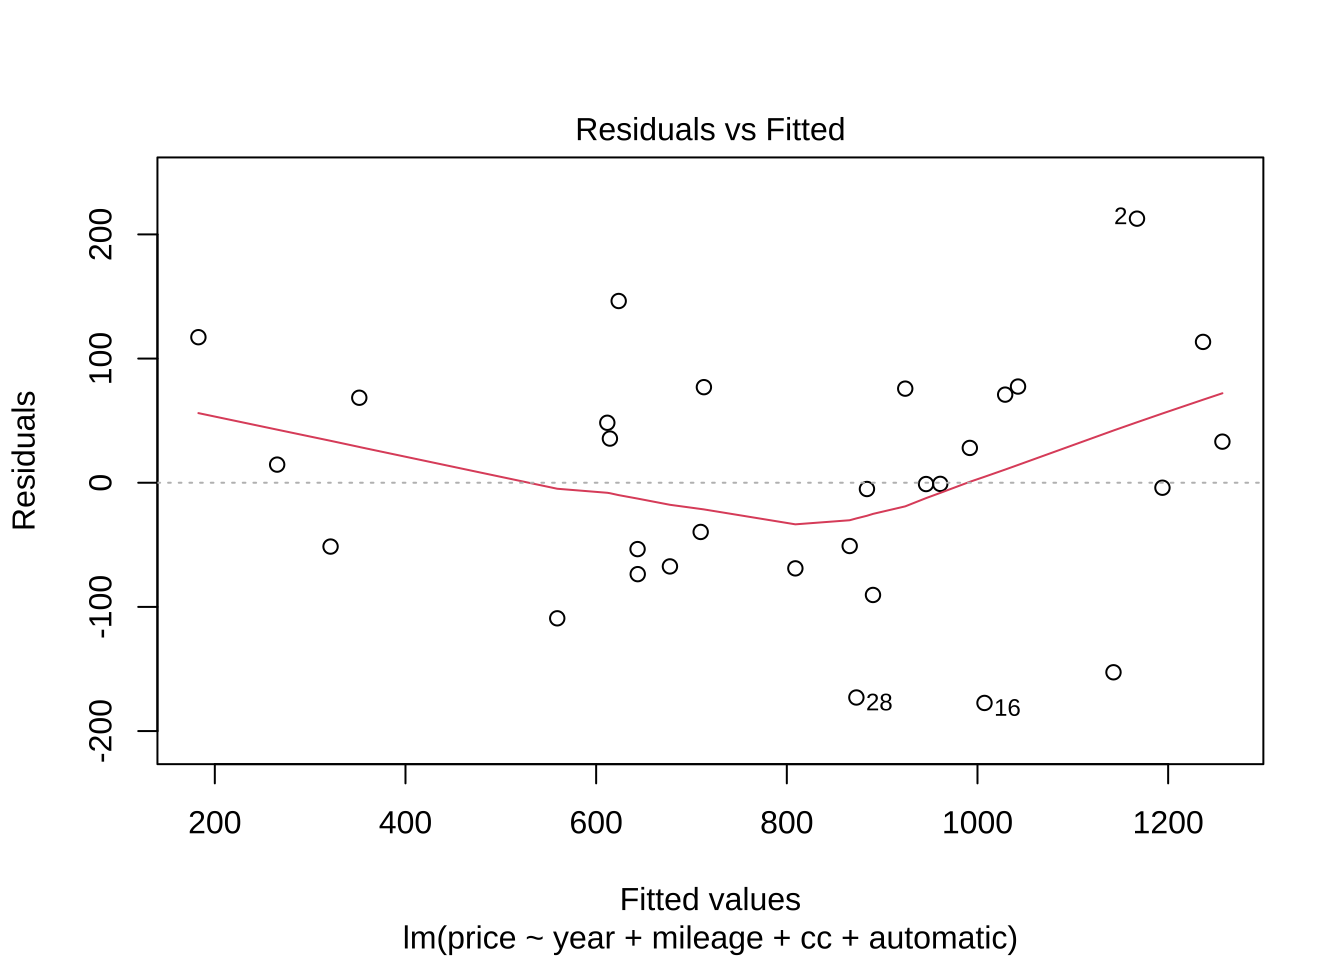
\includegraphics{lmpractice_files/figure-latex/unnamed-chunk-54-1.pdf} 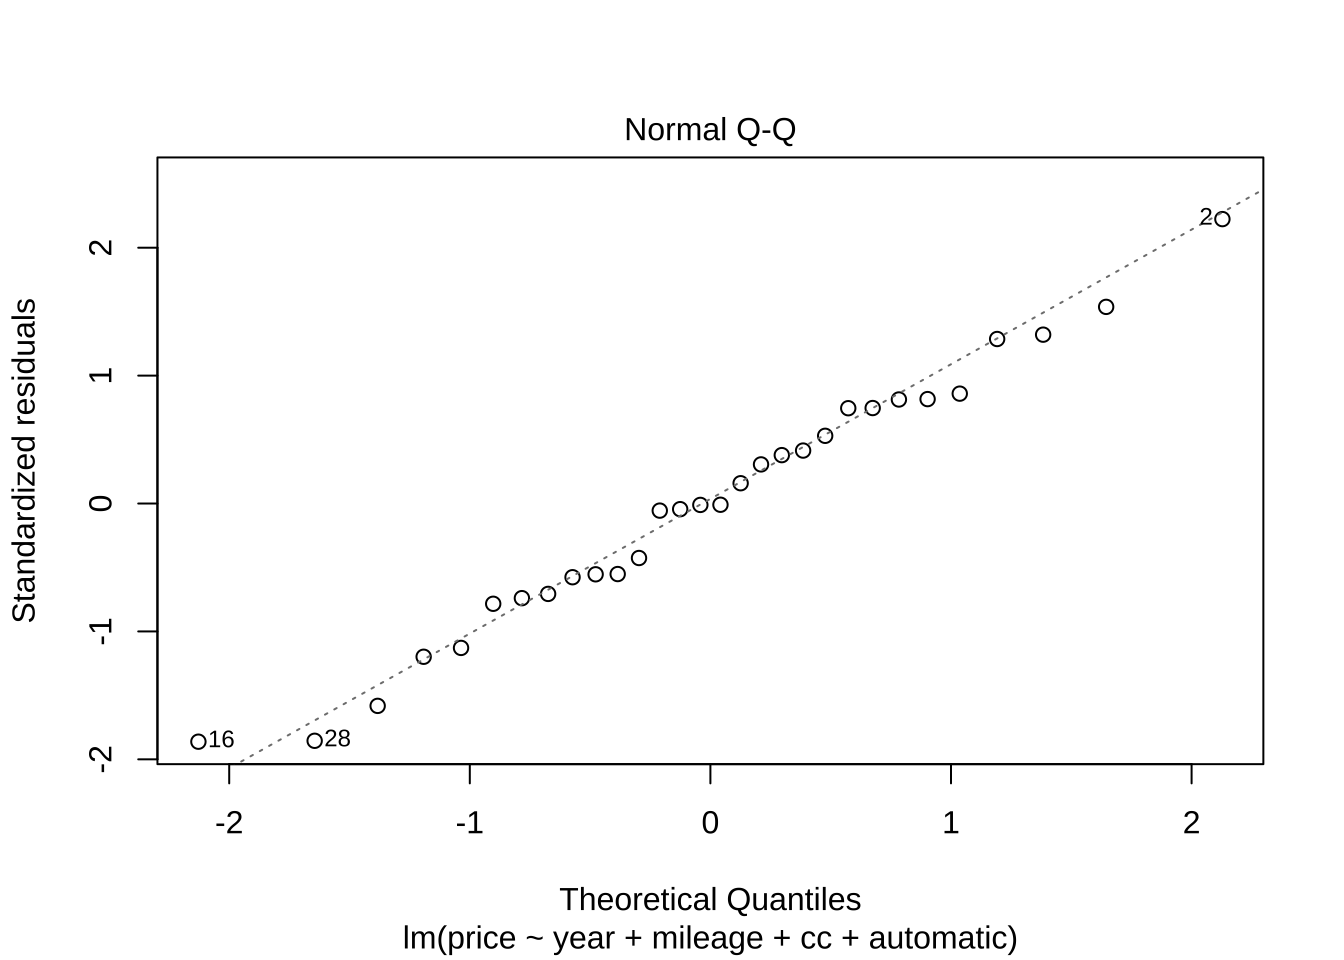
\includegraphics{lmpractice_files/figure-latex/unnamed-chunk-54-2.pdf} 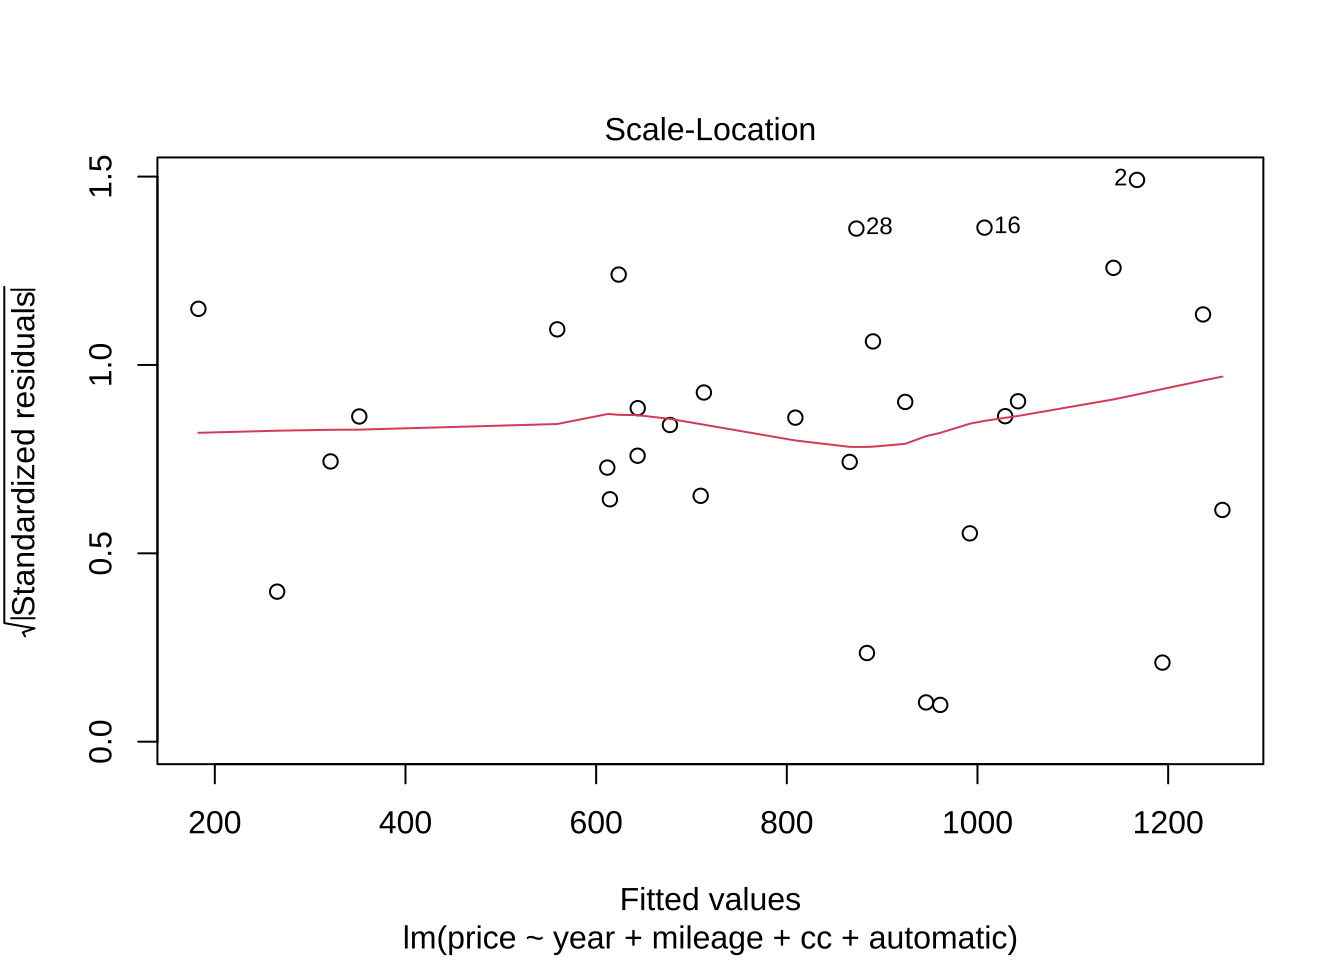
\includegraphics{lmpractice_files/figure-latex/unnamed-chunk-54-3.pdf} 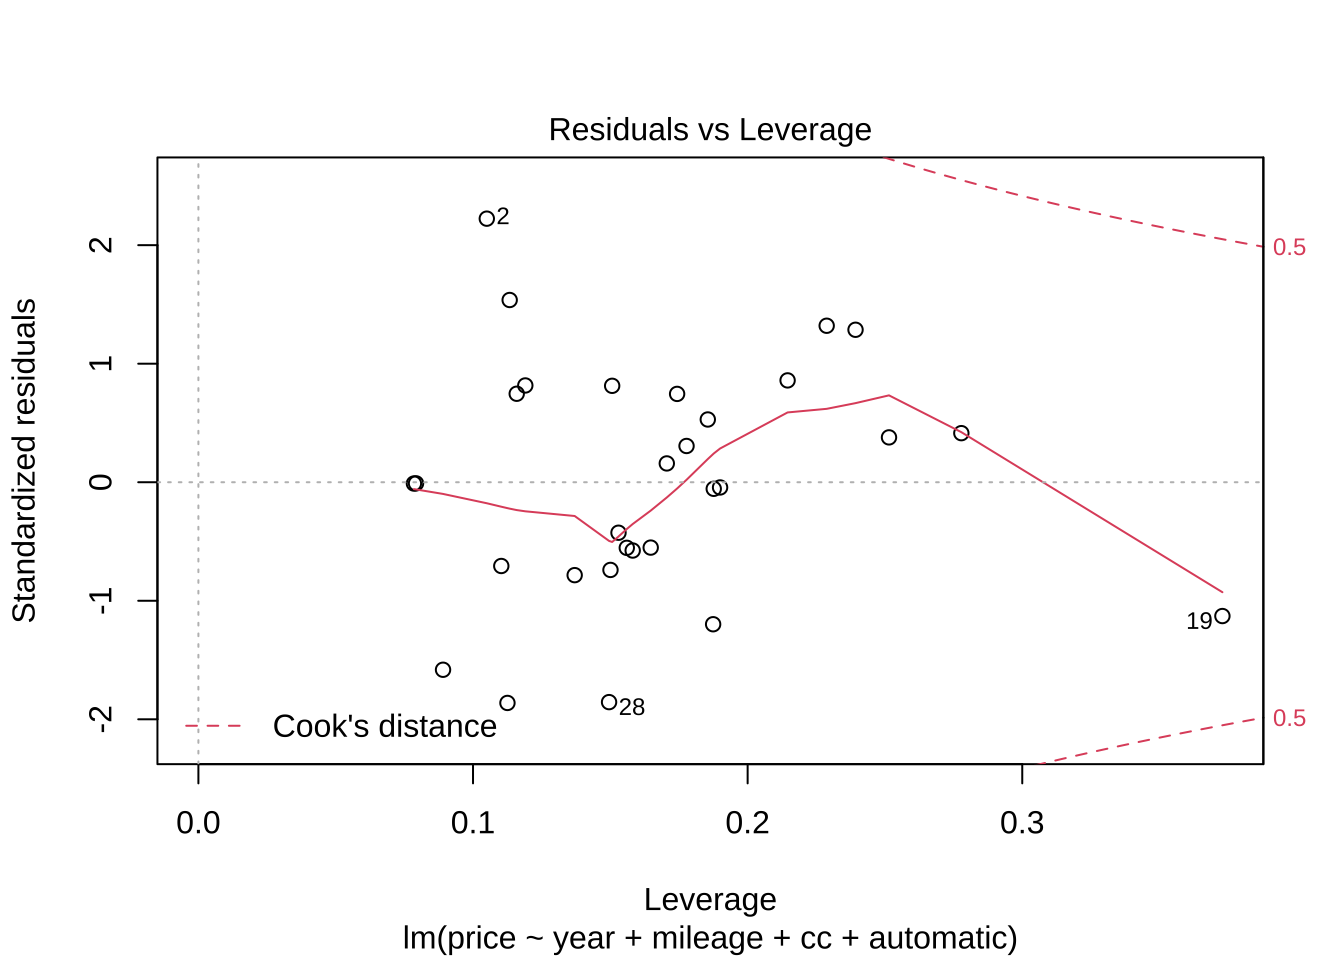
\includegraphics{lmpractice_files/figure-latex/unnamed-chunk-54-4.pdf}

\hypertarget{uxc794uxcc28}{%
\subsection{잔차}\label{uxc794uxcc28}}

\begin{Shaded}
\begin{Highlighting}[]
\NormalTok{resid\_inter }\OtherTok{\textless{}{-}} \FunctionTok{rstandard}\NormalTok{(usedcars.lm)  }\CommentTok{\# internal studentized residual}
\NormalTok{resid\_exter }\OtherTok{\textless{}{-}} \FunctionTok{rstudent}\NormalTok{(usedcars.lm)   }\CommentTok{\# external studentized residual}
\NormalTok{hatval }\OtherTok{\textless{}{-}} \FunctionTok{hatvalues}\NormalTok{(usedcars.lm)       }\CommentTok{\# leverage}
\FunctionTok{data.frame}\NormalTok{(resid\_inter , resid\_exter, hatval)}
\end{Highlighting}
\end{Shaded}

\begin{verbatim}
##     resid_inter  resid_exter     hatval
## 1   0.859118727  0.854468915 0.21455013
## 2   2.223678962  2.432560486 0.10501551
## 3  -0.553417436 -0.545588388 0.15599165
## 4  -0.044084943 -0.043195925 0.18996253
## 5  -0.576180936 -0.568325835 0.15814304
## 6   0.816421059  0.810807796 0.11903880
## 7  -0.551399974 -0.543574935 0.16470220
## 8  -1.198080391 -1.209098031 0.18743332
## 9   0.378399054  0.371820157 0.25147525
## 10  0.745189938  0.738380670 0.17431785
## 11 -0.010873657 -0.010653990 0.07847932
## 12  1.537452127  1.583088042 0.11334881
## 13 -0.706665346 -0.699408397 0.11029244
## 14  1.286252868  1.304157036 0.23928783
## 15  0.305838319  0.300221293 0.17774944
## 16 -1.862061057 -1.965848316 0.11253640
## 17 -0.425962246 -0.418878889 0.15297508
## 18 -1.582023043 -1.634007936 0.08908012
## 19 -1.128902196 -1.135412108 0.37287989
## 20  0.746526192  0.739734875 0.11591279
## 21 -0.739861832 -0.732982630 0.15005336
## 22 -0.783820912 -0.777598695 0.13701582
## 23  0.529387292  0.521623446 0.18549015
## 24  1.320232140  1.341155689 0.22878139
## 25 -0.009531759 -0.009339195 0.07924745
## 26  0.414031097  0.407063963 0.27781733
## 27  0.813419294  0.807745473 0.15066704
## 28 -1.855054061 -1.957267375 0.14953912
## 29  0.158642701  0.155515766 0.17056129
## 30 -0.055408868 -0.054292716 0.18765466
\end{verbatim}

\hypertarget{uxc601uxd5a5uxc810-uxce21uxb3c4}{%
\subsection{영향점 측도}\label{uxc601uxd5a5uxc810-uxce21uxb3c4}}

\begin{Shaded}
\begin{Highlighting}[]
\CommentTok{\# DFBETAS for each model variable, DFFITS, covariance ratios, }
\CommentTok{\# Cook\textquotesingle{}s distances and the diagonal elements of the hat matrix}
\CommentTok{\# Cases which are influential with respect to any of these measures }
\CommentTok{\# are marked with an asterisk.}
\FunctionTok{influence.measures}\NormalTok{(usedcars.lm)}
\end{Highlighting}
\end{Shaded}

\begin{verbatim}
## Influence measures of
##   lm(formula = price ~ year + mileage + cc + automatic, data = usedcars) :
## 
##      dfb.1_  dfb.year  dfb.milg   dfb.cc dfb.atmt    dffit cov.r   cook.d    hat inf
## 1  -0.20716 -0.108544  0.327125  0.17932  0.19256  0.44658 1.344 4.03e-02 0.2146    
## 2  -0.18773  0.033416 -0.347354  0.24746  0.23435  0.83326 0.455 1.16e-01 0.1050    
## 3  -0.10302 -0.086990  0.008925  0.10950  0.06372 -0.23455 1.366 1.13e-02 0.1560    
## 4   0.00469  0.016237 -0.011729 -0.00589 -0.00320 -0.02092 1.513 9.12e-05 0.1900    
## 5   0.11228  0.102465 -0.135083 -0.12498  0.13462 -0.24632 1.363 1.25e-02 0.1581    
## 6  -0.07885  0.136480 -0.181209  0.08714  0.11239  0.29805 1.216 1.80e-02 0.1190    
## 7  -0.14228  0.100579 -0.106201  0.14682 -0.10174 -0.24137 1.381 1.20e-02 0.1647    
## 8  -0.27687  0.308498 -0.320654  0.25704  0.24993 -0.58070 1.123 6.62e-02 0.1874    
## 9   0.15471 -0.066016 -0.054370 -0.13883  0.03146  0.21551 1.592 9.62e-03 0.2515    
## 10  0.13093 -0.056206  0.169173 -0.13765 -0.10220  0.33927 1.328 2.34e-02 0.1743    
## 11  0.00143 -0.000670  0.000312 -0.00142 -0.00166 -0.00311 1.331 2.01e-06 0.0785    
## 12 -0.27881  0.085189 -0.022194  0.31082 -0.33867  0.56603 0.842 6.04e-02 0.1133    
## 13  0.10909 -0.027792  0.028700 -0.12774  0.15983 -0.24625 1.246 1.24e-02 0.1103    
## 14  0.52930 -0.229975 -0.166587 -0.47750  0.11713  0.73144 1.145 1.04e-01 0.2393    
## 15 -0.02434 -0.037299 -0.032166  0.04432 -0.10023  0.13959 1.464 4.04e-03 0.1777    
## 16 -0.47183  0.092199  0.101866  0.45460 -0.29124 -0.70004 0.655 8.79e-02 0.1125    
## 17  0.08120 -0.112348  0.030779 -0.06848 -0.09956 -0.17801 1.396 6.55e-03 0.1530    
## 18  0.14607  0.138551  0.019412 -0.18052 -0.15882 -0.51098 0.795 4.90e-02 0.0891    
## 19  0.08767 -0.454297  0.733107 -0.15988  0.36621 -0.87551 1.505 1.52e-01 0.3729    
## 20  0.17302 -0.084980  0.007572 -0.16482  0.10281  0.26785 1.239 1.46e-02 0.1159    
## 21  0.14757  0.081228 -0.204480 -0.13332 -0.13993 -0.30798 1.292 1.93e-02 0.1501    
## 22 -0.21369 -0.011866  0.084126  0.19253  0.16353 -0.30984 1.255 1.95e-02 0.1370    
## 23 -0.12798  0.071546  0.083597  0.10512  0.13711  0.24893 1.423 1.28e-02 0.1855    
## 24  0.22299  0.430646 -0.103308 -0.26300 -0.09994  0.73047 1.108 1.03e-01 0.2288    
## 25  0.00129  0.000354 -0.000686 -0.00128 -0.00137 -0.00274 1.332 1.56e-06 0.0792    
## 26  0.06915  0.204983 -0.141142 -0.08585  0.12561  0.25248 1.641 1.32e-02 0.2778   *
## 27 -0.08134 -0.093035 -0.048156  0.12751 -0.25004  0.34021 1.263 2.35e-02 0.1507    
## 28  0.28532 -0.571184  0.447521 -0.26551 -0.37866 -0.82073 0.688 1.21e-01 0.1495    
## 29  0.02625  0.019365  0.010861 -0.02922 -0.01619  0.07052 1.471 1.04e-03 0.1706    
## 30  0.00732  0.016726 -0.010214 -0.01018  0.01709 -0.02609 1.509 1.42e-04 0.1877
\end{verbatim}

\hypertarget{uxbd80uxbd84uxd68cuxadc0uxadf8uxb9bc}{%
\subsection{부분회귀그림}\label{uxbd80uxbd84uxd68cuxadc0uxadf8uxb9bc}}

\begin{Shaded}
\begin{Highlighting}[]
\CommentTok{\#added variable plot}
\FunctionTok{avPlots}\NormalTok{(usedcars.lm)}
\end{Highlighting}
\end{Shaded}

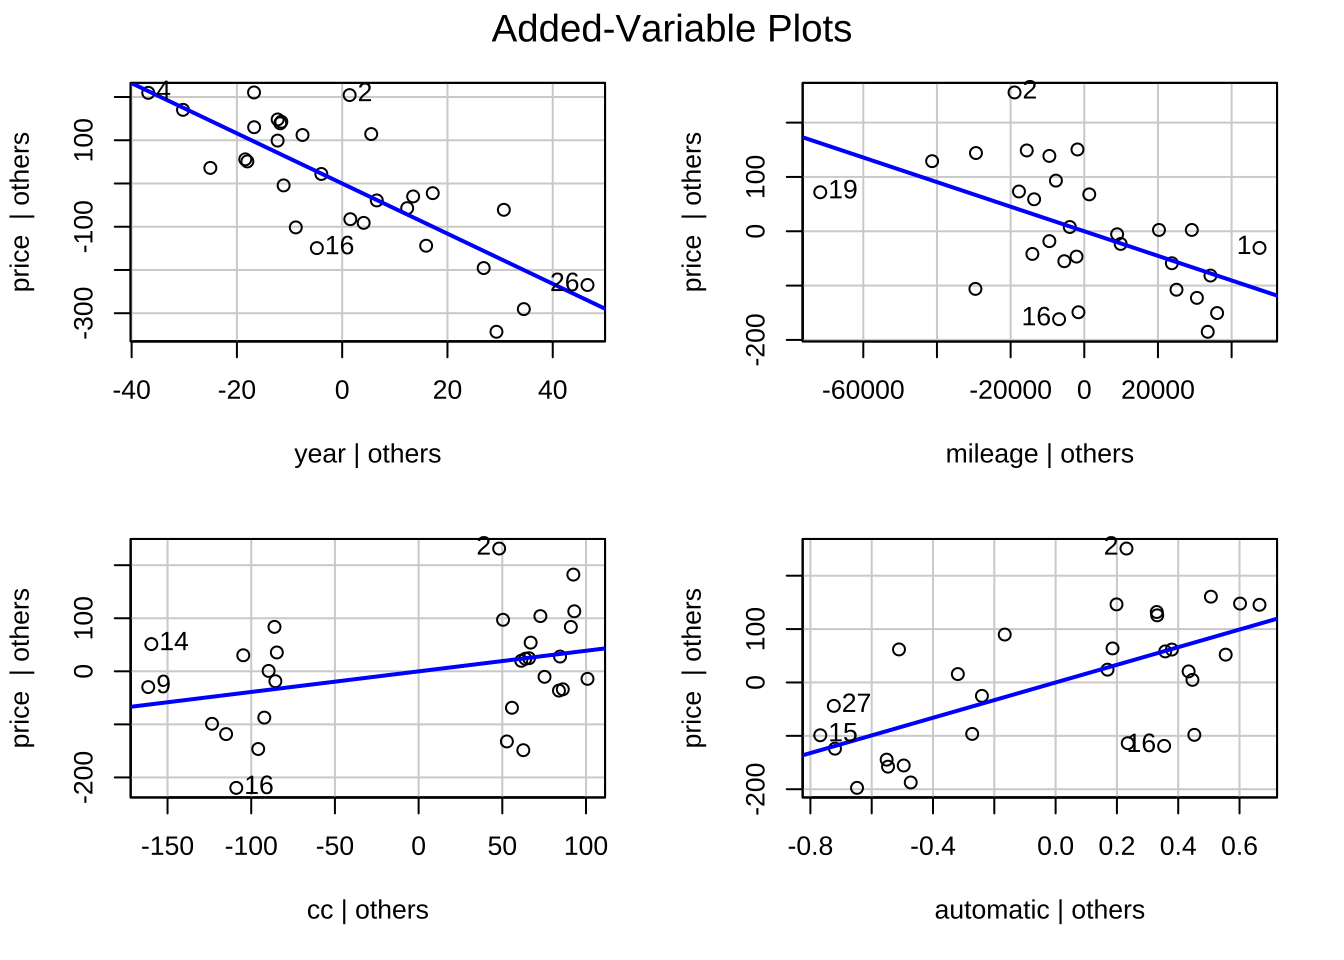
\includegraphics{lmpractice_files/figure-latex/unnamed-chunk-57-1.pdf}

\hypertarget{uxc790uxb8cc-houseprice-uxc5d0-uxb300uxd55c-uxc794uxcc28-uxbd84uxc11d-uxc5f0uxc2b5uxbb38uxc81c-5.9}{%
\section{\texorpdfstring{자료 \texttt{houseprice} 에 대한 잔차 분석 (연습문제 5.9)}{자료 houseprice 에 대한 잔차 분석 (연습문제 5.9)}}\label{uxc790uxb8cc-houseprice-uxc5d0-uxb300uxd55c-uxc794uxcc28-uxbd84uxc11d-uxc5f0uxc2b5uxbb38uxc81c-5.9}}

\begin{itemize}
\tightlist
\item
  \texttt{price} : 주택 판매가격(천만원)
\item
  \texttt{tax} : 세금(만원)
\item
  \texttt{ground} : 대지평수(평)
\item
  \texttt{floor} : 건물평수(평)
\item
  \texttt{year} : 주택연령(년)
\end{itemize}

\begin{Shaded}
\begin{Highlighting}[]
\NormalTok{house.lm }\OtherTok{\textless{}{-}} \FunctionTok{lm}\NormalTok{(price }\SpecialCharTok{\textasciitilde{}}\NormalTok{ tax }\SpecialCharTok{+}\NormalTok{ ground }\SpecialCharTok{+}\NormalTok{ floor }\SpecialCharTok{+}\NormalTok{ year, houseprice)}
\FunctionTok{summary}\NormalTok{(house.lm )}
\end{Highlighting}
\end{Shaded}

\begin{verbatim}
## 
## Call:
## lm(formula = price ~ tax + ground + floor + year, data = houseprice)
## 
## Residuals:
##     Min      1Q  Median      3Q     Max 
## -3.4891 -1.3574  0.1337  1.0686  3.4938 
## 
## Coefficients:
##             Estimate Std. Error t value Pr(>|t|)    
## (Intercept)  1.21874    2.04661   0.595  0.55759    
## tax          0.05195    0.01383   3.756  0.00109 ** 
## ground       0.01159    0.02534   0.458  0.65169    
## floor        0.34941    0.07268   4.807 8.41e-05 ***
## year        -0.21894    0.33149  -0.660  0.51582    
## ---
## Signif. codes:  0 '***' 0.001 '**' 0.01 '*' 0.05 '.' 0.1 ' ' 1
## 
## Residual standard error: 2.039 on 22 degrees of freedom
## Multiple R-squared:  0.9313, Adjusted R-squared:  0.9188 
## F-statistic: 74.53 on 4 and 22 DF,  p-value: 1.817e-12
\end{verbatim}

\hypertarget{uxc794uxcc28uxadf8uxb9bc-1}{%
\subsection{잔차그림}\label{uxc794uxcc28uxadf8uxb9bc-1}}

\begin{Shaded}
\begin{Highlighting}[]
\FunctionTok{plot}\NormalTok{(house.lm)}
\end{Highlighting}
\end{Shaded}

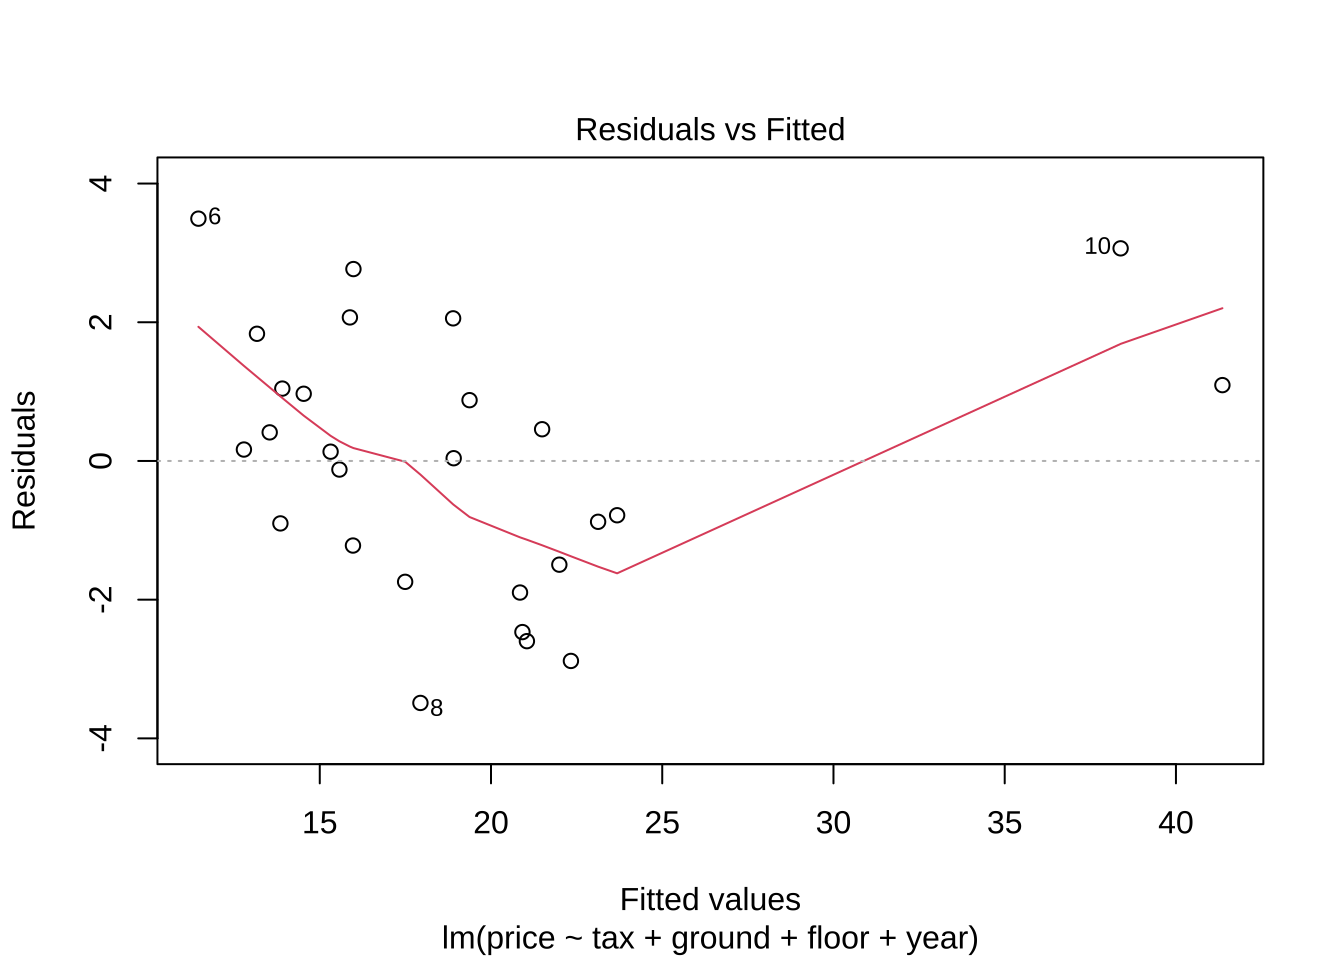
\includegraphics{lmpractice_files/figure-latex/unnamed-chunk-59-1.pdf} 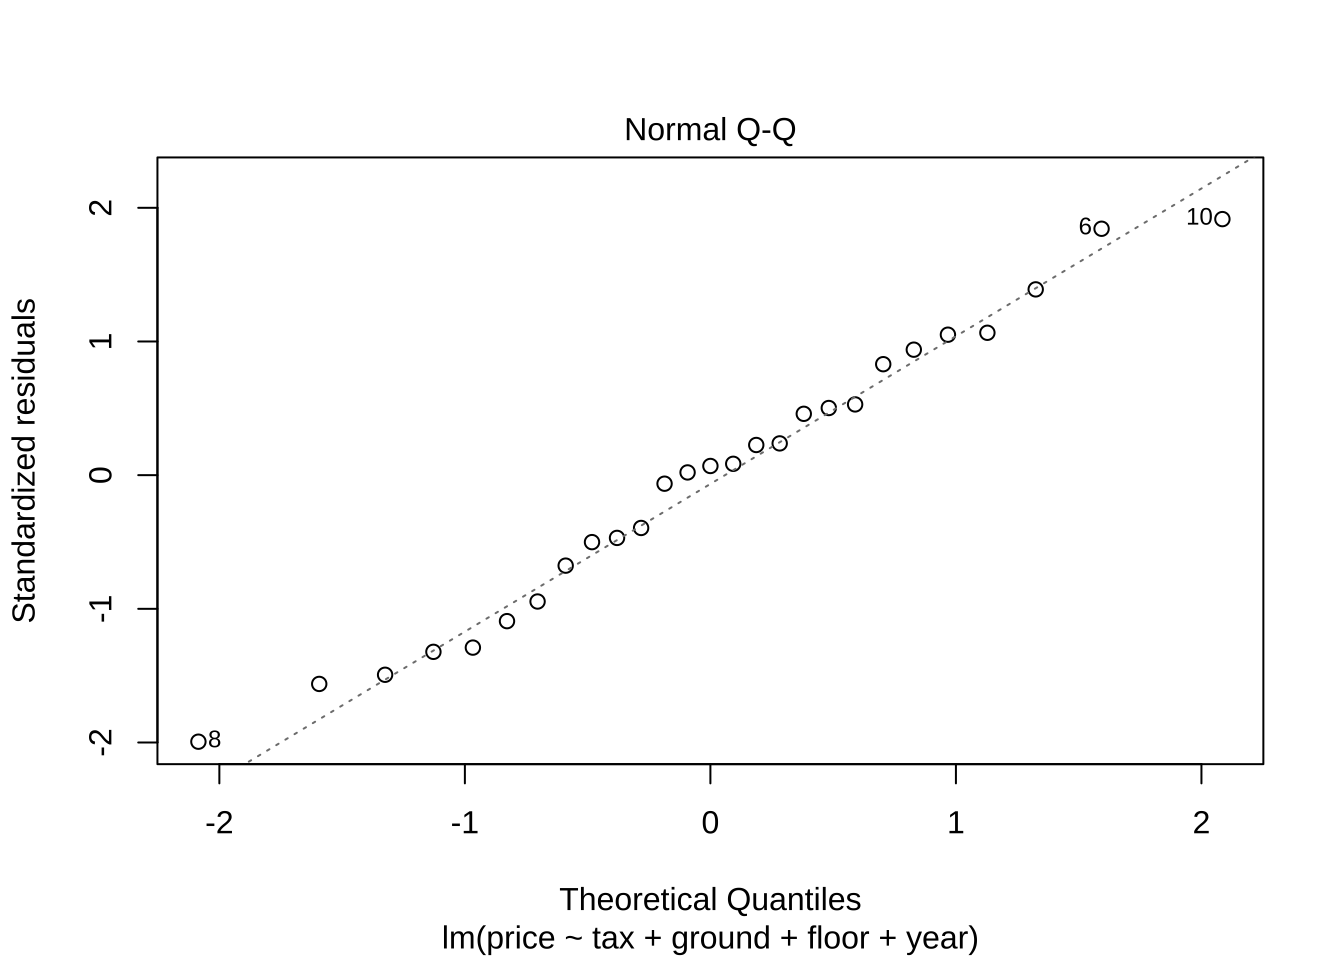
\includegraphics{lmpractice_files/figure-latex/unnamed-chunk-59-2.pdf} 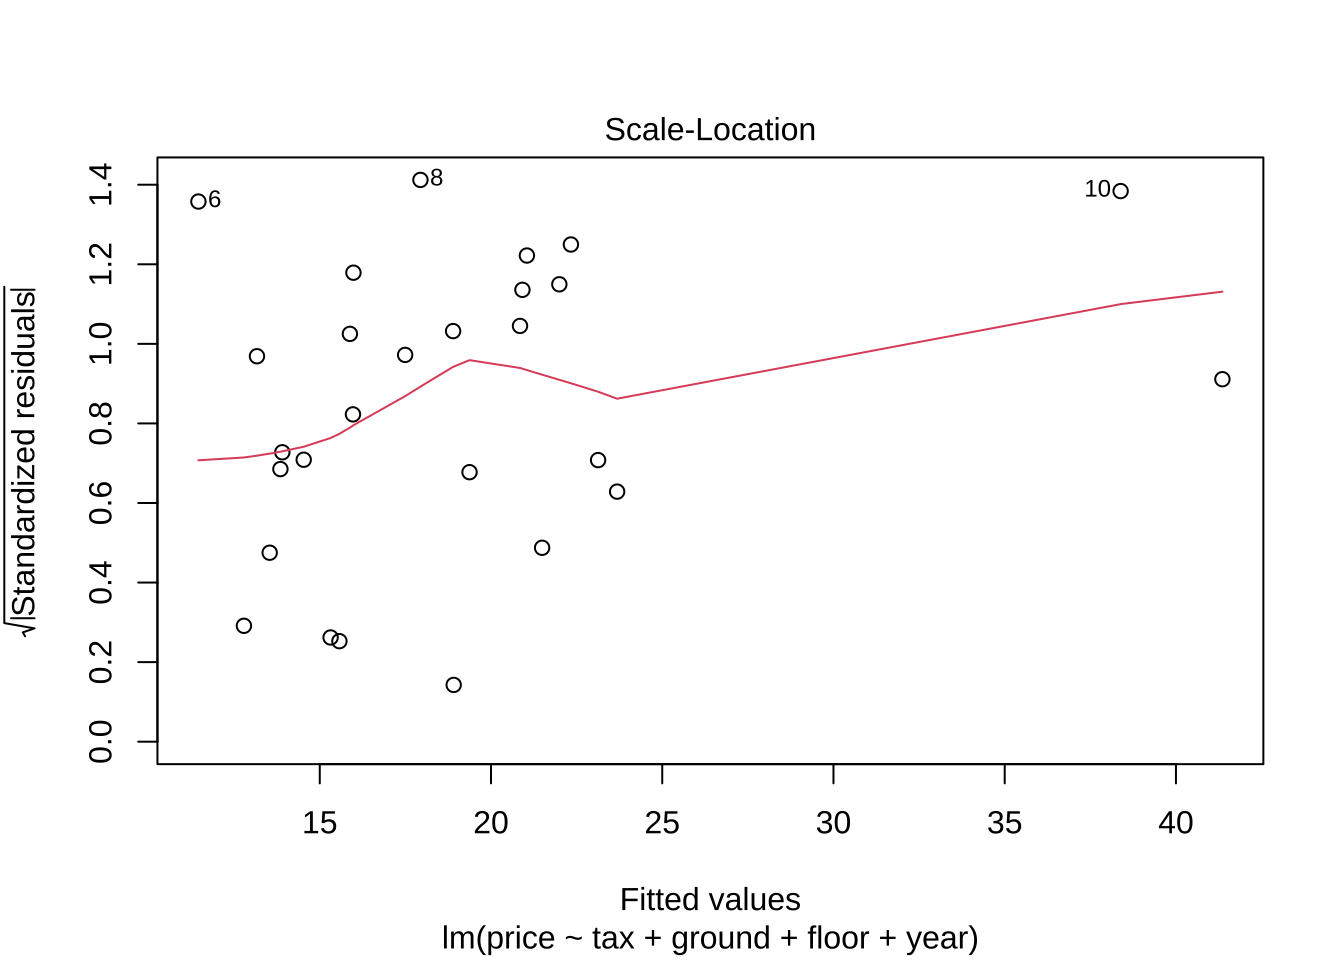
\includegraphics{lmpractice_files/figure-latex/unnamed-chunk-59-3.pdf} 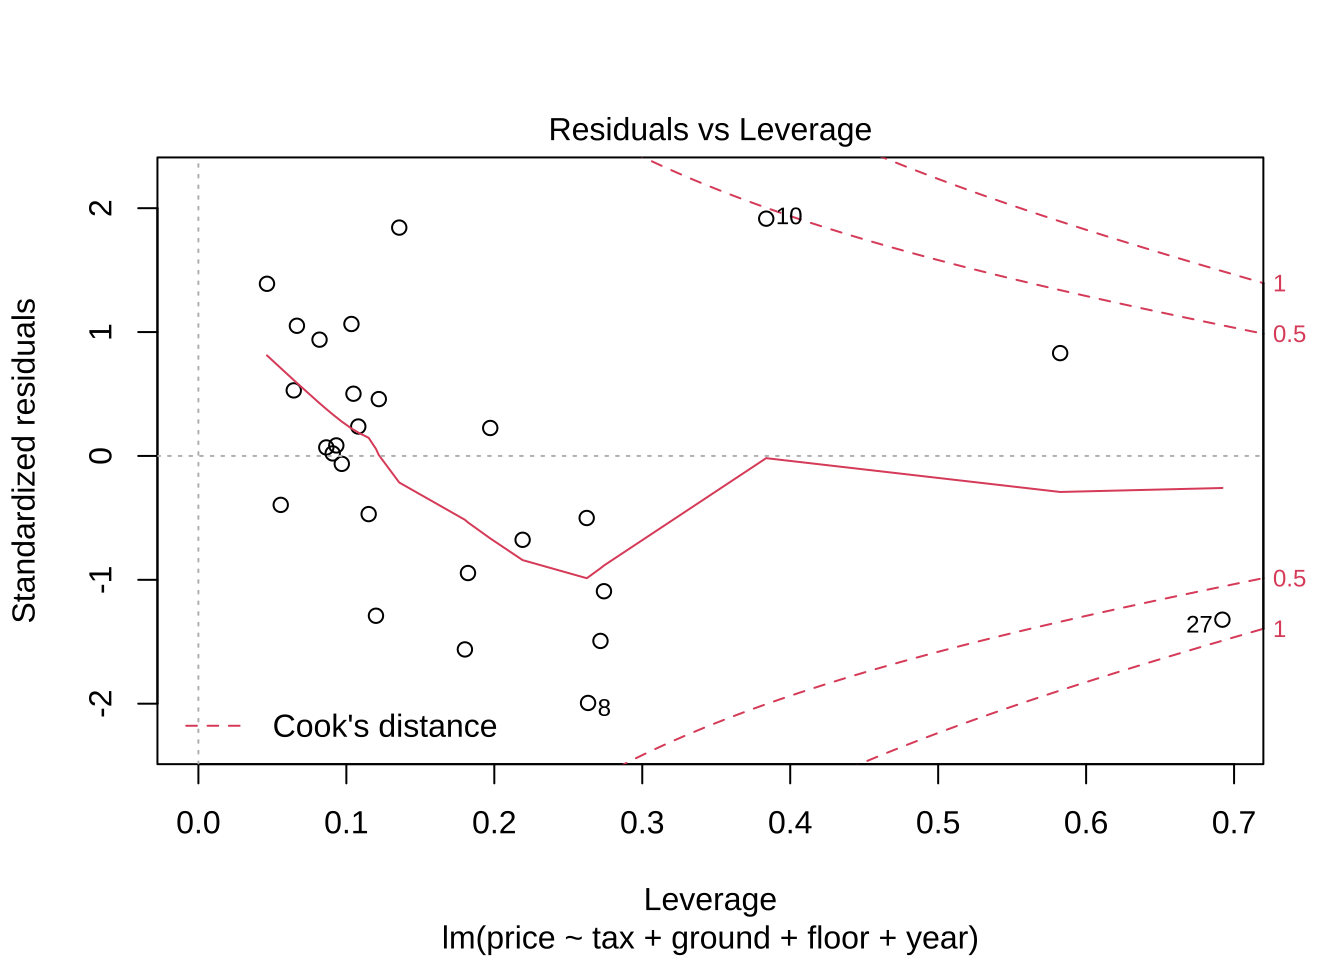
\includegraphics{lmpractice_files/figure-latex/unnamed-chunk-59-4.pdf}

\hypertarget{uxc794uxcc28-1}{%
\subsection{잔차}\label{uxc794uxcc28-1}}

\begin{Shaded}
\begin{Highlighting}[]
\NormalTok{resid\_inter }\OtherTok{\textless{}{-}} \FunctionTok{rstandard}\NormalTok{(house.lm)  }\CommentTok{\# internal studentized residual}
\NormalTok{resid\_exter }\OtherTok{\textless{}{-}} \FunctionTok{rstudent}\NormalTok{(house.lm)   }\CommentTok{\# external studentized residual}
\NormalTok{hatval }\OtherTok{\textless{}{-}} \FunctionTok{hatvalues}\NormalTok{(house.lm)       }\CommentTok{\# leverage}
\FunctionTok{data.frame}\NormalTok{(resid\_inter , resid\_exter, hatval)}
\end{Highlighting}
\end{Shaded}

\begin{verbatim}
##    resid_inter resid_exter     hatval
## 1   0.08485161  0.08291431 0.09320631
## 2  -0.67688158 -0.66831473 0.21913894
## 3   0.22562538  0.22069338 0.19724713
## 4  -0.46948020 -0.46100124 0.11507835
## 5   0.52919554  0.52035100 0.06445355
## 6   1.84331217  1.95851264 0.13574846
## 7  -0.06384170 -0.06237966 0.09690865
## 8  -1.99395355 -2.15227270 0.26336419
## 9   0.83013951  0.82406251 0.58244898
## 10  1.91549041  2.05020730 0.38378669
## 11  1.05080043  1.05341670 0.06658106
## 12 -0.94527321 -0.94288627 0.18220181
## 13  0.50227319  0.49356319 0.10480032
## 14  0.06861447  0.06704409 0.08643549
## 15  0.93871235  0.93606793 0.08186844
## 16 -1.29008121 -1.31098352 0.12001347
## 17  1.06516817  1.06859785 0.10343469
## 18  0.45890058  0.45051112 0.12193265
## 19  0.23755461  0.23239110 0.10805628
## 20  1.38973242  1.42161443 0.04635041
## 21 -1.09213214 -1.09717908 0.27411620
## 22 -0.50097821 -0.49227596 0.26244274
## 23  0.02037349  0.01990526 0.09076853
## 24 -1.56186889 -1.61831671 0.18011950
## 25 -1.49330686 -1.53905802 0.27174557
## 26 -0.39509397 -0.38738692 0.05564326
## 27 -1.32177835 -1.34593675 0.69210833
\end{verbatim}

\hypertarget{uxc601uxd5a5uxc810-uxce21uxb3c4-1}{%
\subsection{영향점 측도}\label{uxc601uxd5a5uxc810-uxce21uxb3c4-1}}

\begin{Shaded}
\begin{Highlighting}[]
\CommentTok{\# DFBETAS for each model variable, DFFITS, covariance ratios, }
\CommentTok{\# Cook\textquotesingle{}s distances and the diagonal elements of the hat matrix}
\CommentTok{\# Cases which are influential with respect to any of these measures }
\CommentTok{\# are marked with an asterisk.}
\FunctionTok{influence.measures}\NormalTok{(house.lm)}
\end{Highlighting}
\end{Shaded}

\begin{verbatim}
## Influence measures of
##   lm(formula = price ~ tax + ground + floor + year, data = houseprice) :
## 
##       dfb.1_   dfb.tax dfb.grnd dfb.flor  dfb.year    dffit cov.r   cook.d    hat inf
## 1   0.014217  0.002017 -0.01275 -0.00268 -0.000135  0.02658 1.389 1.48e-04 0.0932    
## 2   0.042404  0.079930  0.14075 -0.15424 -0.158274 -0.35404 1.455 2.57e-02 0.2191    
## 3   0.069922 -0.027157 -0.08571  0.04958 -0.034094  0.10940 1.554 2.50e-03 0.1972    
## 4  -0.007662  0.042042  0.03758 -0.03751 -0.069086 -0.16624 1.356 5.73e-03 0.1151    
## 5   0.063837 -0.019261 -0.03297 -0.00264  0.006118  0.13658 1.265 3.86e-03 0.0645    
## 6  -0.054546 -0.098819  0.13310 -0.13410  0.454340  0.77620 0.631 1.07e-01 0.1357    
## 7   0.006212 -0.003046 -0.00704  0.00782 -0.014422 -0.02043 1.396 8.75e-05 0.0969    
## 8  -0.005790  0.732398 -1.01363 -0.05094  0.080104 -1.28691 0.632 2.84e-01 0.2634   *
## 9  -0.485623  0.145037 -0.28210  0.47003  0.181974  0.97327 2.578 1.92e-01 0.5824   *
## 10 -0.441587 -0.024860  0.39734  0.44403 -0.383840  1.61800 0.822 4.57e-01 0.3838   *
## 11  0.135462 -0.079420  0.10301 -0.05113 -0.073622  0.28134 1.045 1.58e-02 0.0666    
## 12 -0.290579  0.312281  0.18500 -0.33279  0.268032 -0.44505 1.254 3.98e-02 0.1822    
## 13  0.080276  0.061427  0.01756 -0.11076 -0.027110  0.16887 1.331 5.91e-03 0.1048    
## 14  0.006784 -0.000403  0.01053 -0.01017 -0.001943  0.02062 1.380 8.91e-05 0.0864    
## 15  0.028693  0.027810  0.05281 -0.12180  0.117515  0.27952 1.120 1.57e-02 0.0819    
## 16  0.148557 -0.215769  0.20142  0.00669 -0.261136 -0.48414 0.968 4.54e-02 0.1200    
## 17  0.246376 -0.173013  0.01794  0.10015 -0.265665  0.36296 1.080 2.62e-02 0.1034    
## 18  0.103552  0.009435  0.01415 -0.03784 -0.110898  0.16788 1.370 5.85e-03 0.1219    
## 19  0.014602  0.036836  0.02175 -0.04407 -0.019199  0.08089 1.397 1.37e-03 0.1081    
## 20  0.091734 -0.009786  0.01097 -0.05796  0.042615  0.31341 0.836 1.88e-02 0.0464    
## 21 -0.450615  0.123028  0.53573 -0.37690  0.450929 -0.67424 1.316 9.01e-02 0.2741    
## 22  0.205044 -0.042537 -0.22449  0.10230 -0.199701 -0.29365 1.615 1.79e-02 0.2624    
## 23 -0.000357 -0.003982  0.00133  0.00316  0.000992  0.00629 1.388 8.29e-06 0.0908    
## 24  0.498955 -0.067078 -0.55352  0.21412 -0.497936 -0.75852 0.855 1.07e-01 0.1801    
## 25 -0.628635  0.164535 -0.05777 -0.02051  0.792697 -0.94014 1.015 1.66e-01 0.2717    
## 26 -0.002774 -0.019178  0.01071 -0.01033  0.016113 -0.09403 1.289 1.84e-03 0.0556    
## 27  0.109605 -1.912785  0.46868  1.41138 -0.355827 -2.01796 2.710 7.85e-01 0.6921   *
\end{verbatim}

\begin{Shaded}
\begin{Highlighting}[]
\FunctionTok{data.frame}\NormalTok{(}\FunctionTok{influence.measures}\NormalTok{(house.lm)}\SpecialCharTok{$}\NormalTok{infmat) }\SpecialCharTok{\%\textgreater{}\%} \FunctionTok{arrange}\NormalTok{(}\FunctionTok{desc}\NormalTok{(cook.d))}
\end{Highlighting}
\end{Shaded}

\begin{verbatim}
##           dfb.1_       dfb.tax     dfb.grnd     dfb.flor      dfb.year        dffit     cov.r       cook.d        hat
## 27  0.1096047217 -1.9127853141  0.468676877  1.411381453 -0.3558265703 -2.017960765 2.7098290 7.854588e-01 0.69210833
## 10 -0.4415870543 -0.0248604761  0.397338451  0.444034941 -0.3838396389  1.617995073 0.8224149 4.570343e-01 0.38378669
## 8  -0.0057902619  0.7323984486 -1.013634156 -0.050938912  0.0801037723 -1.286913158 0.6323020 2.842916e-01 0.26336419
## 9  -0.4856234858  0.1450371174 -0.282098491  0.470027818  0.1819741325  0.973272210 2.5775061 1.922563e-01 0.58244898
## 25 -0.6286351847  0.1645351185 -0.057767986 -0.020507197  0.7926966789 -0.940144619 1.0154477 1.664207e-01 0.27174557
## 24  0.4989545517 -0.0670775894 -0.553522590  0.214118018 -0.4979362714 -0.758522754 0.8551849 1.071838e-01 0.18011950
## 6  -0.0545461054 -0.0988187998  0.133102135 -0.134103045  0.4543397926  0.776200207 0.6310808 1.067389e-01 0.13574846
## 21 -0.4506145915  0.1230280032  0.535727211 -0.376896955  0.4509288359 -0.674235034 1.3155567 9.008406e-02 0.27411620
## 16  0.1485568463 -0.2157694362  0.201415137  0.006694886 -0.2611364532 -0.484143630 0.9676585 4.539605e-02 0.12001347
## 12 -0.2905789777  0.3122807716  0.185004213 -0.332794386  0.2680322860 -0.445053871 1.2541060 3.981541e-02 0.18220181
## 17  0.2463756161 -0.1730128116  0.017939895  0.100146357 -0.2656652976  0.362958055 1.0800825 2.617885e-02 0.10343469
## 2   0.0424037098  0.0799299689  0.140753289 -0.154237840 -0.1582742772 -0.354041305 1.4545976 2.571587e-02 0.21913894
## 20  0.0917343695 -0.0097856304  0.010973417 -0.057957406  0.0426148630  0.313410964 0.8358047 1.877401e-02 0.04635041
## 22  0.2050435817 -0.0425371361 -0.224492803  0.102295021 -0.1997011456 -0.293648675 1.6154977 1.786103e-02 0.26244274
## 11  0.1354618103 -0.0794200881  0.103010169 -0.051125306 -0.0736223445  0.281343734 1.0450182 1.575232e-02 0.06658106
## 15  0.0286930080  0.0278098038  0.052808877 -0.121803476  0.1175145249  0.279520178 1.1203321 1.571472e-02 0.08186844
## 13  0.0802759117  0.0614266653  0.017558647 -0.110759188 -0.0271098481  0.168874509 1.3306151 5.906805e-03 0.10480032
## 18  0.1035515927  0.0094345541  0.014153127 -0.037842744 -0.1108978787  0.167881022 1.3696294 5.848701e-03 0.12193265
## 4  -0.0076624989  0.0420420176  0.037576080 -0.037512885 -0.0690856639 -0.166244194 1.3559605 5.732622e-03 0.11507835
## 5   0.0638374271 -0.0192611164 -0.032971284 -0.002640161  0.0061177215  0.136580011 1.2651222 3.858725e-03 0.06445355
## 3   0.0699218586 -0.0271569355 -0.085706412  0.049581510 -0.0340940269  0.109396575 1.5538338 2.501697e-03 0.19724713
## 26 -0.0027742220 -0.0191783392  0.010712437 -0.010330051  0.0161132923 -0.094033628 1.2894913 1.839532e-03 0.05564326
## 19  0.0146019324  0.0368361881  0.021746080 -0.044073810 -0.0191988608  0.080886448 1.3966972 1.367318e-03 0.10805628
## 1   0.0142171388  0.0020173997 -0.012754491 -0.002679822 -0.0001347719  0.026582627 1.3893053 1.480086e-04 0.09320631
## 14  0.0067843423 -0.0004028513  0.010527346 -0.010173078 -0.0019433376  0.020622293 1.3797899 8.908700e-05 0.08643549
## 7   0.0062121502 -0.0030464468 -0.007037304  0.007822060 -0.0144221961 -0.020434236 1.3959920 8.747214e-05 0.09690865
## 23 -0.0003574067 -0.0039823274  0.001330353  0.003161260  0.0009924586  0.006289241 1.3877189 8.287463e-06 0.09076853
\end{verbatim}

\hypertarget{uxbd80uxbd84uxd68cuxadc0uxadf8uxb9bc-1}{%
\subsection{부분회귀그림}\label{uxbd80uxbd84uxd68cuxadc0uxadf8uxb9bc-1}}

\begin{Shaded}
\begin{Highlighting}[]
\CommentTok{\#added variable plot}
\FunctionTok{avPlots}\NormalTok{(house.lm)}
\end{Highlighting}
\end{Shaded}

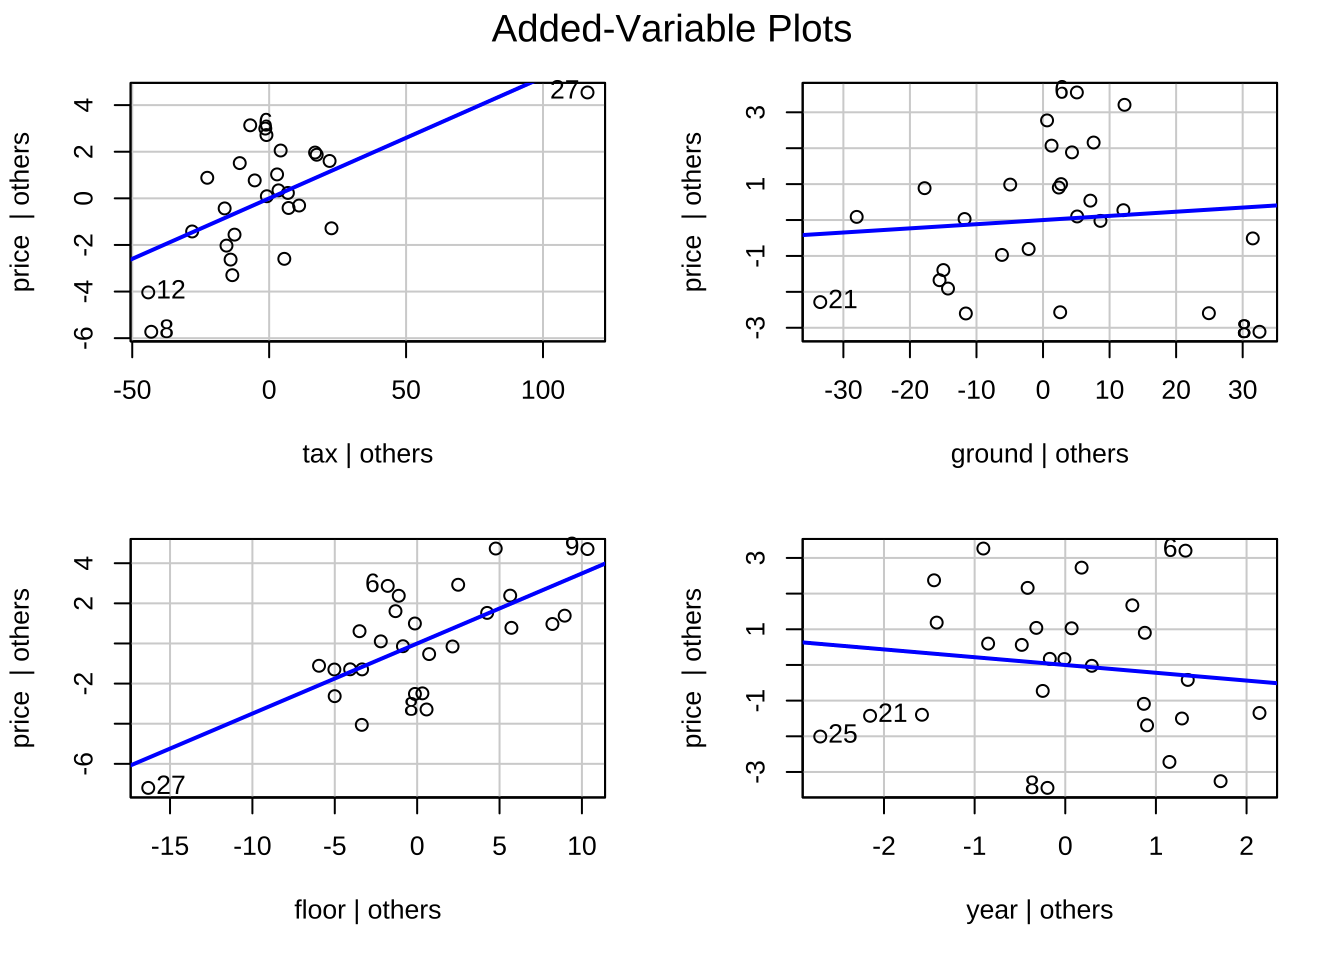
\includegraphics{lmpractice_files/figure-latex/unnamed-chunk-63-1.pdf}

\hypertarget{onewayanova}{%
\chapter{일원배치에서의 추정: 예제와 R 실습}\label{onewayanova}}

\hypertarget{uxc608uxc81c}{%
\section{예제}\label{uxc608uxc81c}}

4개의 서로 다른 원단업체에서 직물을 공급받고 있다. 공급한 직물의 긁힘에
대한 저항력을 알아보기 위하여 각 업체마다 4개의 제품을 랜덤하게 선택하여
(\(a=4\), \(r=4\)) 일원배치법에 의하여 마모도 검사을 실시하였다.

\hypertarget{uxc790uxb8ccuxc758-uxc0dduxc131}{%
\section{자료의 생성}\label{uxc790uxb8ccuxc758-uxc0dduxc131}}

\begin{Shaded}
\begin{Highlighting}[]
\NormalTok{company}\OtherTok{\textless{}{-}} \FunctionTok{as.factor}\NormalTok{(}\FunctionTok{rep}\NormalTok{(}\FunctionTok{c}\NormalTok{(}\DecValTok{1}\SpecialCharTok{:}\DecValTok{4}\NormalTok{), }\AttributeTok{each=}\DecValTok{4}\NormalTok{))}
\NormalTok{response}\OtherTok{\textless{}{-}} \FunctionTok{c}\NormalTok{(}\FloatTok{1.93}\NormalTok{, }\FloatTok{2.38}\NormalTok{, }\FloatTok{2.20}\NormalTok{, }\FloatTok{2.25}\NormalTok{,}
             \FloatTok{2.55}\NormalTok{, }\FloatTok{2.72}\NormalTok{, }\FloatTok{2.75}\NormalTok{, }\FloatTok{2.70}\NormalTok{,}
             \FloatTok{2.40}\NormalTok{, }\FloatTok{2.68}\NormalTok{, }\FloatTok{2.32}\NormalTok{, }\FloatTok{2.28}\NormalTok{,}
             \FloatTok{2.33}\NormalTok{, }\FloatTok{2.38}\NormalTok{, }\FloatTok{2.28}\NormalTok{, }\FloatTok{2.25}\NormalTok{)}
\NormalTok{df31}\OtherTok{\textless{}{-}} \FunctionTok{data.frame}\NormalTok{(}\AttributeTok{company=}\NormalTok{company, }\AttributeTok{response=}\NormalTok{ response)}
\NormalTok{df31}
\end{Highlighting}
\end{Shaded}

\begin{verbatim}
##    company response
## 1        1     1.93
## 2        1     2.38
## 3        1     2.20
## 4        1     2.25
## 5        2     2.55
## 6        2     2.72
## 7        2     2.75
## 8        2     2.70
## 9        3     2.40
## 10       3     2.68
## 11       3     2.32
## 12       3     2.28
## 13       4     2.33
## 14       4     2.38
## 15       4     2.28
## 16       4     2.25
\end{verbatim}

각 수준에 대한 표보 평균을 구해보자.

\begin{Shaded}
\begin{Highlighting}[]
\NormalTok{df31s }\OtherTok{\textless{}{-}}\NormalTok{ df31 }\SpecialCharTok{\%\textgreater{}\%} \FunctionTok{group\_by}\NormalTok{(company)  }\SpecialCharTok{\%\textgreater{}\%}  \FunctionTok{summarise}\NormalTok{(}\AttributeTok{mean=}\FunctionTok{mean}\NormalTok{(response), }\AttributeTok{median=} \FunctionTok{median}\NormalTok{(response), }\AttributeTok{sd=}\FunctionTok{sd}\NormalTok{(response), }\AttributeTok{min=}\FunctionTok{min}\NormalTok{(response), }\AttributeTok{max=}\FunctionTok{max}\NormalTok{(response))}
\NormalTok{df31s}
\end{Highlighting}
\end{Shaded}

\begin{verbatim}
## # A tibble: 4 x 6
##   company  mean median     sd   min   max
##   <fct>   <dbl>  <dbl>  <dbl> <dbl> <dbl>
## 1 1        2.19   2.22 0.189   1.93  2.38
## 2 2        2.68   2.71 0.0891  2.55  2.75
## 3 3        2.42   2.36 0.180   2.28  2.68
## 4 4        2.31   2.30 0.0572  2.25  2.38
\end{verbatim}

\hypertarget{uxc120uxd615uxbaa8uxd615uxc758-uxc801uxd569set-to-zero}{%
\section{선형모형의 적합(set-to-zero)}\label{uxc120uxd615uxbaa8uxd615uxc758-uxc801uxd569set-to-zero}}

이제 자료를 다음과 같은 선형 모형으로 적합해 보자. 선형 모형의 적합은
\texttt{lm()} 함수를 사용한다.

\[ y_{ij} = \mu + \alpha_i + e_{ij}  \]

여기서 선형식의 모수와 \texttt{R}의 변수는 다음과 같은 관계를 가진다,

\begin{longtable}[]{@{}rr@{}}
\toprule
선형식의 모수 & \texttt{R}의 변수\tabularnewline
\midrule
\endhead
\(\mu\) & \texttt{(Intercept)}\tabularnewline
\(\alpha_1\) & \texttt{company1}\tabularnewline
\(\alpha_2\) & \texttt{company2}\tabularnewline
\(\alpha_3\) & \texttt{company3}\tabularnewline
\(\alpha_4\) & \texttt{company4}\tabularnewline
\bottomrule
\end{longtable}

\begin{Shaded}
\begin{Highlighting}[]
\NormalTok{fit1 }\OtherTok{\textless{}{-}} \FunctionTok{lm}\NormalTok{(response}\SpecialCharTok{\textasciitilde{}}\NormalTok{company,}\AttributeTok{data=}\NormalTok{df31)}
\FunctionTok{summary}\NormalTok{(fit1)}
\end{Highlighting}
\end{Shaded}

\begin{verbatim}
## 
## Call:
## lm(formula = response ~ company, data = df31)
## 
## Residuals:
##     Min      1Q  Median      3Q     Max 
## -0.2600 -0.0700  0.0150  0.0625  0.2600 
## 
## Coefficients:
##             Estimate Std. Error t value Pr(>|t|)    
## (Intercept)  2.19000    0.07050  31.062 7.79e-13 ***
## company2     0.49000    0.09971   4.914 0.000357 ***
## company3     0.23000    0.09971   2.307 0.039710 *  
## company4     0.12000    0.09971   1.204 0.251982    
## ---
## Signif. codes:  0 '***' 0.001 '**' 0.01 '*' 0.05 '.' 0.1 ' ' 1
## 
## Residual standard error: 0.141 on 12 degrees of freedom
## Multiple R-squared:  0.6871, Adjusted R-squared:  0.6089 
## F-statistic: 8.785 on 3 and 12 DF,  p-value: 0.002353
\end{verbatim}

위에서 적합한 결과를 보면 평균 \(\mu\)와 4개의 처리 \(\alpha_1\),
\(\alpha_2\), \(\alpha_3\), \(\alpha_4\) 가 모형에 있지만 모수의 추정량은
평균(\texttt{intercept})과 3개의 모수(\texttt{company2}, \texttt{company3}, \texttt{company4})만
추정량이 주어진다.

\texttt{R} 에서 옵션을 지정하지 않고 함수 \texttt{lm()}으로 선형모형을 적합하는 경우 set-to-zero 조건을
적용하며 자료에 나타난 처리의 수준들 중 순위가 가장 낮은 수준의 효과를
0으로 지정한다 (\texttt{company1}=0 ). set-to-zero 조건을 강제로 지정하려면 다음과 같은 명령문을 먼저 실행한다.

\begin{verbatim}
options(contrasts=c("contr.treatment", "contr.poly"))
\end{verbatim}

위의 결과를 보면 \texttt{(Intercept)}에 대한 추정량이 첫 번째 처리 \texttt{company1}의
평균과 같은 것을 알 수 있다.

set-to-zero 조건에서의 계획행렬은 다음과 같이 볼 수 있다.

\begin{Shaded}
\begin{Highlighting}[]
\FunctionTok{model.matrix}\NormalTok{(fit1)}
\end{Highlighting}
\end{Shaded}

\begin{verbatim}
##    (Intercept) company2 company3 company4
## 1            1        0        0        0
## 2            1        0        0        0
## 3            1        0        0        0
## 4            1        0        0        0
## 5            1        1        0        0
## 6            1        1        0        0
## 7            1        1        0        0
## 8            1        1        0        0
## 9            1        0        1        0
## 10           1        0        1        0
## 11           1        0        1        0
## 12           1        0        1        0
## 13           1        0        0        1
## 14           1        0        0        1
## 15           1        0        0        1
## 16           1        0        0        1
## attr(,"assign")
## [1] 0 1 1 1
## attr(,"contrasts")
## attr(,"contrasts")$company
## [1] "contr.treatment"
\end{verbatim}

이제 각 처리 평균에 대한 추정값 \(\widehat{\mu+ \alpha_i}\)을 구해보자.

\begin{Shaded}
\begin{Highlighting}[]
\FunctionTok{emmeans}\NormalTok{(fit1, }\StringTok{"company"}\NormalTok{)}
\end{Highlighting}
\end{Shaded}

\begin{verbatim}
##  company emmean     SE df lower.CL upper.CL
##  1         2.19 0.0705 12     2.04     2.34
##  2         2.68 0.0705 12     2.53     2.83
##  3         2.42 0.0705 12     2.27     2.57
##  4         2.31 0.0705 12     2.16     2.46
## 
## Confidence level used: 0.95
\end{verbatim}

이 경우 처리 평균에 대한 추정값은 산술 평균과 동일하게 나온다.

\hypertarget{uxc120uxd615uxbaa8uxd615uxc758-uxc801uxd569-sum-to-zero}{%
\section{선형모형의 적합 (sum-to-zero)}\label{uxc120uxd615uxbaa8uxd615uxc758-uxc801uxd569-sum-to-zero}}

이제 일원배치 모형에서 sum-to-zero 조건을 적용하여 모수를 추정해 보자.
sum-to-zero 조건을 적용하려면 다음과 같은 명령어를 실행해야 한다.

\begin{Shaded}
\begin{Highlighting}[]
\FunctionTok{options}\NormalTok{(}\AttributeTok{contrasts=}\FunctionTok{c}\NormalTok{(}\StringTok{"contr.sum"}\NormalTok{, }\StringTok{"contr.poly"}\NormalTok{))}
\end{Highlighting}
\end{Shaded}

이제 다시 선형모형을 적합하고 추정결과를 보자.

\begin{Shaded}
\begin{Highlighting}[]
\NormalTok{fit2 }\OtherTok{\textless{}{-}} \FunctionTok{lm}\NormalTok{(response}\SpecialCharTok{\textasciitilde{}}\NormalTok{company,}\AttributeTok{data=}\NormalTok{df31)}
\FunctionTok{summary}\NormalTok{(fit2)}
\end{Highlighting}
\end{Shaded}

\begin{verbatim}
## 
## Call:
## lm(formula = response ~ company, data = df31)
## 
## Residuals:
##     Min      1Q  Median      3Q     Max 
## -0.2600 -0.0700  0.0150  0.0625  0.2600 
## 
## Coefficients:
##             Estimate Std. Error t value Pr(>|t|)    
## (Intercept)  2.40000    0.03525  68.081  < 2e-16 ***
## company1    -0.21000    0.06106  -3.439 0.004901 ** 
## company2     0.28000    0.06106   4.586 0.000626 ***
## company3     0.02000    0.06106   0.328 0.748892    
## ---
## Signif. codes:  0 '***' 0.001 '**' 0.01 '*' 0.05 '.' 0.1 ' ' 1
## 
## Residual standard error: 0.141 on 12 degrees of freedom
## Multiple R-squared:  0.6871, Adjusted R-squared:  0.6089 
## F-statistic: 8.785 on 3 and 12 DF,  p-value: 0.002353
\end{verbatim}

이제 sum-to-zero 조건에 따라서 위의 set-to-zero 결과와 모수의 추정값이
다르게 나타나는 것을 알 수 있다. 마지막 모수 \texttt{company4}(\(\alpha_4\))는
sum-to-zero 조건을 이용하여 다음과 같은 관계를 이용하여 구할 수 있다.

\[  \alpha_4 = -(\alpha_1 + \alpha_2 + \alpha_3) \]

sum-to-zero 조건에서의 계획행렬은 다음과 같이 볼 수 있다.

\begin{Shaded}
\begin{Highlighting}[]
\FunctionTok{model.matrix}\NormalTok{(fit2)}
\end{Highlighting}
\end{Shaded}

\begin{verbatim}
##    (Intercept) company1 company2 company3
## 1            1        1        0        0
## 2            1        1        0        0
## 3            1        1        0        0
## 4            1        1        0        0
## 5            1        0        1        0
## 6            1        0        1        0
## 7            1        0        1        0
## 8            1        0        1        0
## 9            1        0        0        1
## 10           1        0        0        1
## 11           1        0        0        1
## 12           1        0        0        1
## 13           1       -1       -1       -1
## 14           1       -1       -1       -1
## 15           1       -1       -1       -1
## 16           1       -1       -1       -1
## attr(,"assign")
## [1] 0 1 1 1
## attr(,"contrasts")
## attr(,"contrasts")$company
## [1] "contr.sum"
\end{verbatim}

이제 각 처리 평균에 대한 추정값 \(\widehat{\mu+ \alpha_i}\)을 구해보면 set-to-zero 조건에서의 추정값과 동일함을 알 수 있다.

\begin{Shaded}
\begin{Highlighting}[]
\FunctionTok{emmeans}\NormalTok{(fit2, }\StringTok{"company"}\NormalTok{)}
\end{Highlighting}
\end{Shaded}

\begin{verbatim}
##  company emmean     SE df lower.CL upper.CL
##  1         2.19 0.0705 12     2.04     2.34
##  2         2.68 0.0705 12     2.53     2.83
##  3         2.42 0.0705 12     2.27     2.57
##  4         2.31 0.0705 12     2.16     2.46
## 
## Confidence level used: 0.95
\end{verbatim}

\hypertarget{uxbd84uxc0b0uxbd84uxc11d}{%
\section{분산분석}\label{uxbd84uxc0b0uxbd84uxc11d}}

분산분석의 결과는 어떠한 제약 조건에서도 동일하다.

\begin{Shaded}
\begin{Highlighting}[]
\NormalTok{res1 }\OtherTok{\textless{}{-}} \FunctionTok{anova}\NormalTok{(fit1)}
\NormalTok{res1}
\end{Highlighting}
\end{Shaded}

\begin{verbatim}
## Analysis of Variance Table
## 
## Response: response
##           Df Sum Sq  Mean Sq F value   Pr(>F)   
## company    3 0.5240 0.174667  8.7846 0.002353 **
## Residuals 12 0.2386 0.019883                    
## ---
## Signif. codes:  0 '***' 0.001 '**' 0.01 '*' 0.05 '.' 0.1 ' ' 1
\end{verbatim}

\begin{Shaded}
\begin{Highlighting}[]
\NormalTok{res2}\OtherTok{\textless{}{-}} \FunctionTok{anova}\NormalTok{(fit2)}
\NormalTok{res2}
\end{Highlighting}
\end{Shaded}

\begin{verbatim}
## Analysis of Variance Table
## 
## Response: response
##           Df Sum Sq  Mean Sq F value   Pr(>F)   
## company    3 0.5240 0.174667  8.7846 0.002353 **
## Residuals 12 0.2386 0.019883                    
## ---
## Signif. codes:  0 '***' 0.001 '**' 0.01 '*' 0.05 '.' 0.1 ' ' 1
\end{verbatim}

\hypertarget{uxb2e4uxc911uxbe44uxad50-uxc608uxc81c}{%
\section{다중비교 예제}\label{uxb2e4uxc911uxbe44uxad50-uxc608uxc81c}}

앞에서 살펴본 일원배치법 예제은 4개의 처리가 있다. 따라서 \({4 \choose 2} =6\)
개의 가설 검정(또는 신뢰구간)을 수행해야 한다.

4개의 \texttt{company}가 처리 수준이며 각 처리수준 은 \texttt{1}, \texttt{2}, \texttt{3}, \texttt{4}로 표시된다.

\begin{Shaded}
\begin{Highlighting}[]
\NormalTok{df31s}
\end{Highlighting}
\end{Shaded}

\begin{verbatim}
## # A tibble: 4 x 6
##   company  mean median     sd   min   max
##   <fct>   <dbl>  <dbl>  <dbl> <dbl> <dbl>
## 1 1        2.19   2.22 0.189   1.93  2.38
## 2 2        2.68   2.71 0.0891  2.55  2.75
## 3 3        2.42   2.36 0.180   2.28  2.68
## 4 4        2.31   2.30 0.0572  2.25  2.38
\end{verbatim}

\hypertarget{uxb2e4uxc911uxbe44uxad50-uxbc29uxbc95uxc744-uxc801uxc6a9uxd558uxc9c0-uxc54auxb294-uxacbduxc6b0}{%
\subsection{다중비교 방법을 적용하지 않는 경우}\label{uxb2e4uxc911uxbe44uxad50-uxbc29uxbc95uxc744-uxc801uxc6a9uxd558uxc9c0-uxc54auxb294-uxacbduxc6b0}}

먼저 다중비교 방법을 적용하지 않는 경우 결과를 보자. 함수 \texttt{LSD.test}
에서 \texttt{p.adj=c("none")}를 지정하면 다중 비교를 적용하지 않는다. 명령문
\texttt{p.adj} 를 지정하지 않으면 수정을 하지 않는 LSD 방법에 의한 신뢰 구간
\eqref{eq:twomeanci} 와 검정 방법 \eqref{eq:lsd}로 구한 결과를 준다.

\begin{Shaded}
\begin{Highlighting}[]
\NormalTok{anova.res }\OtherTok{\textless{}{-}} \FunctionTok{aov}\NormalTok{(response}\SpecialCharTok{\textasciitilde{}}\NormalTok{company,}\AttributeTok{data=}\NormalTok{df31) }\CommentTok{\#일원배치}
\NormalTok{test1 }\OtherTok{\textless{}{-}} \FunctionTok{LSD.test}\NormalTok{(anova.res, }\StringTok{"company"}\NormalTok{, }\AttributeTok{alpha =} \FloatTok{0.05}\NormalTok{, }\AttributeTok{group =} \ConstantTok{FALSE}\NormalTok{, }\AttributeTok{console =} \ConstantTok{FALSE}\NormalTok{, }\AttributeTok{p.adj=}\FunctionTok{c}\NormalTok{(}\StringTok{"none"}\NormalTok{) )}
\NormalTok{test1}\SpecialCharTok{$}\NormalTok{comparison}
\end{Highlighting}
\end{Shaded}

\begin{verbatim}
##       difference pvalue signif.         LCL         UCL
## 1 - 2      -0.49 0.0004     *** -0.70724487 -0.27275513
## 1 - 3      -0.23 0.0397       * -0.44724487 -0.01275513
## 1 - 4      -0.12 0.2520         -0.33724487  0.09724487
## 2 - 3       0.26 0.0229       *  0.04275513  0.47724487
## 2 - 4       0.37 0.0030      **  0.15275513  0.58724487
## 3 - 4       0.11 0.2916         -0.10724487  0.32724487
\end{verbatim}

\hypertarget{uxbcf8uxd398uxb85cuxb2c8-uxc218uxc815bonferroni-correction}{%
\subsection{본페로니 수정(Bonferroni correction)}\label{uxbcf8uxd398uxb85cuxb2c8-uxc218uxc815bonferroni-correction}}

이제 다중비교 방법 중에 가장 보수적인 본페로니 수정(Bonferroni
correction)을 적용해 보자. 함수 \texttt{LSD.test} 에서
\texttt{p.adj=c("bonferroni")}를 이용한다.

아래의 결과는 본페로니 수정 방법에 의한 신뢰 구간
와 검정 방법으로 구한 결과이다.

본페로니 수정이 적용된 신뢰구간은 LSD 방법의
신뢰구간보다 길며 수정된 p-값은 LSD 방법으로 구한 값의 6배이다. LSD 방법을
적용하는 경우 유의한 차이를 보이는 조합이 4개로
나타났는데(1-2,1-3,2-3,2-4) 본페로니 수정을 적용한 경우에는 2개로 줄어
들었다(1-2,2-4)

수정한 p-값이 1이 초과하면 확률이기 때문에 1로 주어진다.

\begin{Shaded}
\begin{Highlighting}[]
\NormalTok{test2 }\OtherTok{\textless{}{-}} \FunctionTok{LSD.test}\NormalTok{(anova.res, }\StringTok{"company"}\NormalTok{, }\AttributeTok{alpha =} \FloatTok{0.05}\NormalTok{, }\AttributeTok{group =} \ConstantTok{FALSE}\NormalTok{, }\AttributeTok{console =} \ConstantTok{FALSE}\NormalTok{, }\AttributeTok{p.adj=}\FunctionTok{c}\NormalTok{(}\StringTok{"bonferroni"}\NormalTok{) )}
\NormalTok{test2}\SpecialCharTok{$}\NormalTok{comparison}
\end{Highlighting}
\end{Shaded}

\begin{verbatim}
##       difference pvalue signif.         LCL         UCL
## 1 - 2      -0.49 0.0021      ** -0.80434725 -0.17565275
## 1 - 3      -0.23 0.2383         -0.54434725  0.08434725
## 1 - 4      -0.12 1.0000         -0.43434725  0.19434725
## 2 - 3       0.26 0.1374         -0.05434725  0.57434725
## 2 - 4       0.37 0.0179       *  0.05565275  0.68434725
## 3 - 4       0.11 1.0000         -0.20434725  0.42434725
\end{verbatim}

\hypertarget{tukeyuxc758-hsd}{%
\subsection{Tukey의 HSD}\label{tukeyuxc758-hsd}}

함수\texttt{TukeyHSD}는 분산분석을 실행한 결과를 이용하여 다중비교 방법 중 가장
많이 이용되는 Tukey's Honest Significant Difference (HSD) 방법으로
다중비교를 제공한다.

Tukey의 HSD는 너무 보수적인 결과를 주는 본페로니 수정을 개선한 것이다.
따라서 Tukey의 HSD 에서 얻은 결과는 수정하지 않는 LDS 의 결과와 Bonferoni
방법의 중간에 있다고 할 수 있다.

Tukey의 HSD 에서는 본페로니와 유사하게 2개의 조합(1-2,2-4)만이 유의한
차이가 있다고 나타난다.

\begin{Shaded}
\begin{Highlighting}[]
\NormalTok{anova.res }\OtherTok{\textless{}{-}} \FunctionTok{aov}\NormalTok{(response}\SpecialCharTok{\textasciitilde{}}\NormalTok{company,}\AttributeTok{data=}\NormalTok{df31) }\CommentTok{\#일원배치}
\NormalTok{test3 }\OtherTok{\textless{}{-}} \FunctionTok{TukeyHSD}\NormalTok{(anova.res, }\AttributeTok{conf.level =} \FloatTok{0.95}\NormalTok{, }\AttributeTok{ordered=}\ConstantTok{FALSE}\NormalTok{)}
\NormalTok{test3}
\end{Highlighting}
\end{Shaded}

\begin{verbatim}
##   Tukey multiple comparisons of means
##     95% family-wise confidence level
## 
## Fit: aov(formula = response ~ company, data = df31)
## 
## $company
##      diff         lwr         upr     p adj
## 2-1  0.49  0.19397708  0.78602292 0.0017496
## 3-1  0.23 -0.06602292  0.52602292 0.1509207
## 4-1  0.12 -0.17602292  0.41602292 0.6362891
## 3-2 -0.26 -0.55602292  0.03602292 0.0924227
## 4-2 -0.37 -0.66602292 -0.07397708 0.0136804
## 4-3 -0.11 -0.40602292  0.18602292 0.6943908
\end{verbatim}

\begin{Shaded}
\begin{Highlighting}[]
\FunctionTok{plot}\NormalTok{(test3)}
\end{Highlighting}
\end{Shaded}

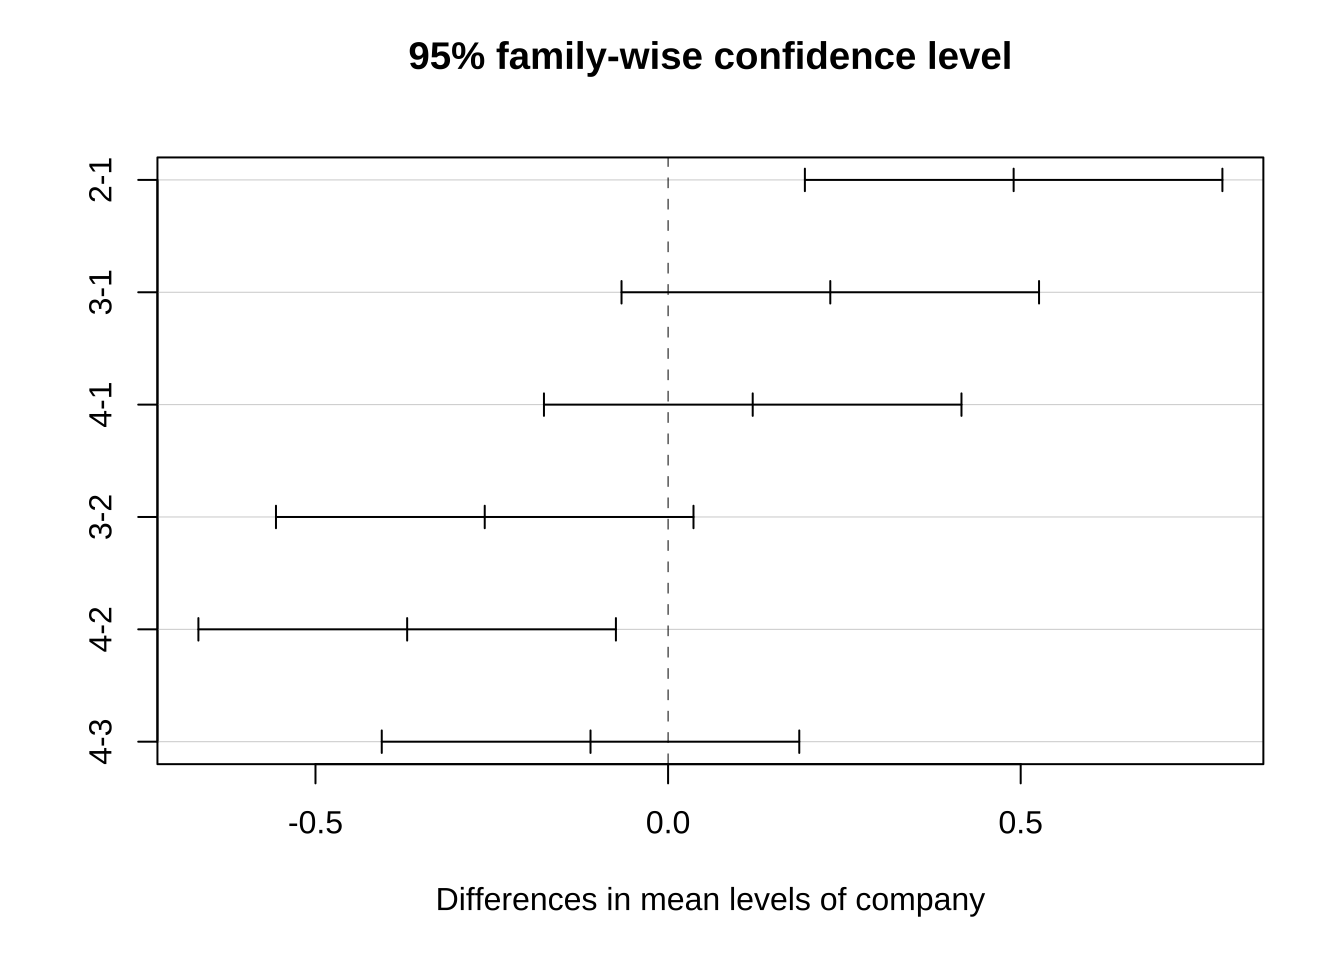
\includegraphics{lmpractice_files/figure-latex/unnamed-chunk-78-1.pdf}

\hypertarget{uxc138-uxbc29uxbc95uxc5d0uxc11cuxc758-p-uxac12-uxbe44uxad50}{%
\subsection{세 방법에서의 p-값 비교}\label{uxc138-uxbc29uxbc95uxc5d0uxc11cuxc758-p-uxac12-uxbe44uxad50}}

위에서 살펴본 수정을 하지 않은 LSD 방법, Tukey의 HSD 방법과 본페로니
방법에서 계산된 p-값을 아래 표에서 비교하였다.

\begin{longtable}[]{@{}rrrr@{}}
\caption{LSD, Bonferoni, HSD 방법의 p-값 비교}\tabularnewline
\toprule
펼균의 비교 조합 & LSD & HSD & Bonf\tabularnewline
\midrule
\endfirsthead
\toprule
펼균의 비교 조합 & LSD & HSD & Bonf\tabularnewline
\midrule
\endhead
1-2 & 0.0004 & 0.0017 & 0.0021\tabularnewline
1-3 & 0.0397 & 0.1509 & 0.2383\tabularnewline
1-4 & 0.2520 & 0.6363 & 1.0000\tabularnewline
2-3 & 0.0229 & 0.0924 & 0.1374\tabularnewline
2-4 & 0.0030 & 0.0137 & 0.0179\tabularnewline
3-4 & 0.2916 & 0.6944 & 1.0000\tabularnewline
\bottomrule
\end{longtable}

\hypertarget{chapter07}{%
\chapter{일웝배치와 공분산분석}\label{chapter07}}

\hypertarget{uxc608uxc81c-7.1---uxc77cuxc6d0uxbc30uxce58}{%
\section{예제 7.1 - 일원배치}\label{uxc608uxc81c-7.1---uxc77cuxc6d0uxbc30uxce58}}

이제 교재 예제 7.1 (271 페이지)에서 관고비 자료 \texttt{adsale}에서 판매액을 예측하는 회귀식을 고려해 보자.

먼저 \texttt{adsale} 데이터프레임에서 두 변수 광고비 \texttt{ad} 와 매체 \texttt{media} 변수의 차이점을 알아보자. 먼저 광고비 \texttt{ad}는 수치 변수(numeric variable)로서 함수 \texttt{class()}를 이용하면 정수(integer) 형태인 것을 알 수 있다. 수치변수는 정수, 실수, 복소수 등을 의미한다.

반면 매체 \texttt{media} 는 범주형 변수로서 함수 \texttt{class()}를 이용하면 범주형(factor) 형태인 것을 알 수 있다. \texttt{levels}는 범주형 변수의 항목을 나타내는 것으로서 범주형 변수 \texttt{media}는 두 개의 항목 \texttt{방송}과 \texttt{신문}으로 이루어 졌음을 알 수 있다.

\begin{Shaded}
\begin{Highlighting}[]
\FunctionTok{head}\NormalTok{(adsale)}
\end{Highlighting}
\end{Shaded}

\begin{verbatim}
##   sale ad media
## 1   39  4  방송
## 2   42  6  신문
## 3   45  6  방송
## 4   47  8  신문
## 5   50  8  방송
## 6   50  9  신문
\end{verbatim}

\begin{Shaded}
\begin{Highlighting}[]
\NormalTok{adsale}\SpecialCharTok{$}\NormalTok{ad}
\end{Highlighting}
\end{Shaded}

\begin{verbatim}
##  [1]  4  6  6  8  8  9  9 10 12 12
\end{verbatim}

\begin{Shaded}
\begin{Highlighting}[]
\NormalTok{adsale}\SpecialCharTok{$}\NormalTok{media}
\end{Highlighting}
\end{Shaded}

\begin{verbatim}
##  [1] 방송 신문 방송 신문 방송 신문 방송 방송 신문 방송
## Levels: 방송 신문
\end{verbatim}

\begin{Shaded}
\begin{Highlighting}[]
\FunctionTok{class}\NormalTok{(adsale}\SpecialCharTok{$}\NormalTok{ad)}
\end{Highlighting}
\end{Shaded}

\begin{verbatim}
## [1] "integer"
\end{verbatim}

\begin{Shaded}
\begin{Highlighting}[]
\FunctionTok{class}\NormalTok{(adsale}\SpecialCharTok{$}\NormalTok{media)}
\end{Highlighting}
\end{Shaded}

\begin{verbatim}
## [1] "factor"
\end{verbatim}

그룹별 기초통계량을 계산해보자.

\begin{Shaded}
\begin{Highlighting}[]
\NormalTok{adsalesum }\OtherTok{\textless{}{-}}\NormalTok{ adsale }\SpecialCharTok{\%\textgreater{}\%} \FunctionTok{group\_by}\NormalTok{(media)  }\SpecialCharTok{\%\textgreater{}\%}  \FunctionTok{summarise}\NormalTok{(}\AttributeTok{mean=}\FunctionTok{mean}\NormalTok{(ad), }\AttributeTok{median=} \FunctionTok{median}\NormalTok{(ad), }\AttributeTok{sd=}\FunctionTok{sd}\NormalTok{(ad), }\AttributeTok{min=}\FunctionTok{min}\NormalTok{(ad), }\AttributeTok{max=}\FunctionTok{max}\NormalTok{(ad))}
\NormalTok{adsalesum}
\end{Highlighting}
\end{Shaded}

\begin{verbatim}
## # A tibble: 2 x 6
##   media  mean median    sd   min   max
##   <fct> <dbl>  <dbl> <dbl> <int> <int>
## 1 방송   8.17    8.5  2.86     4    12
## 2 신문   8.75    8.5  2.5      6    12
\end{verbatim}

함수 lm()으로 선형모형을 적합하는 경우 set-to-zero 조건을 적용하며 자료에 나타난 처리의 수준들 중 순위가 가장 낮은 수준의 효과를 0으로 지정한다 set-to-zero 조건을 강제로 지정하려면 다음과 같은 명령문을 먼저 실행한다.

\begin{Shaded}
\begin{Highlighting}[]
\FunctionTok{options}\NormalTok{(}\AttributeTok{contrasts=}\FunctionTok{c}\NormalTok{(}\StringTok{"contr.treatment"}\NormalTok{, }\StringTok{"contr.poly"}\NormalTok{))}
\end{Highlighting}
\end{Shaded}

이제 광고비 \texttt{ad} 와 매체 \texttt{media} 를 포함한 회귀식을 적합시켜 보자. \texttt{R}의 \texttt{lm} 함수는
범주형변수를 자동적으로 가변수로 바꾸어 준다. 회귀식에 사용된 디자인행렬을 보면 \texttt{media}에 해당하는 열이 0 과 1로 이루어진 벡터로 바뀌었음을 알 수 있다.

\begin{Shaded}
\begin{Highlighting}[]
\NormalTok{fit1 }\OtherTok{\textless{}{-}} \FunctionTok{lm}\NormalTok{(sale}\SpecialCharTok{\textasciitilde{}}\NormalTok{ ad }\SpecialCharTok{+}\NormalTok{ media, }\AttributeTok{data=}\NormalTok{adsale)}
\FunctionTok{summary}\NormalTok{(fit1)}
\end{Highlighting}
\end{Shaded}

\begin{verbatim}
## 
## Call:
## lm(formula = sale ~ ad + media, data = adsale)
## 
## Residuals:
##      Min       1Q   Median       3Q      Max 
## -0.47902 -0.24720  0.02727  0.22832  0.39091 
## 
## Coefficients:
##             Estimate Std. Error t value Pr(>|t|)    
## (Intercept) 29.21888    0.38588   75.72 1.84e-11 ***
## ad           2.56503    0.04408   58.19 1.16e-10 ***
## media신문   -2.66294    0.22114  -12.04 6.21e-06 ***
## ---
## Signif. codes:  0 '***' 0.001 '**' 0.01 '*' 0.05 '.' 0.1 ' ' 1
## 
## Residual standard error: 0.3403 on 7 degrees of freedom
## Multiple R-squared:  0.998,  Adjusted R-squared:  0.9974 
## F-statistic:  1707 on 2 and 7 DF,  p-value: 3.875e-10
\end{verbatim}

\begin{Shaded}
\begin{Highlighting}[]
\FunctionTok{model.matrix}\NormalTok{(fit1)}
\end{Highlighting}
\end{Shaded}

\begin{verbatim}
##    (Intercept) ad media신문
## 1            1  4         0
## 2            1  6         1
## 3            1  6         0
## 4            1  8         1
## 5            1  8         0
## 6            1  9         1
## 7            1  9         0
## 8            1 10         0
## 9            1 12         1
## 10           1 12         0
## attr(,"assign")
## [1] 0 1 2
## attr(,"contrasts")
## attr(,"contrasts")$media
## [1] "contr.treatment"
\end{verbatim}

\begin{Shaded}
\begin{Highlighting}[]
\FunctionTok{data.frame}\NormalTok{(}\AttributeTok{media=}\NormalTok{adsale}\SpecialCharTok{$}\NormalTok{media, }\AttributeTok{z=}\FunctionTok{model.matrix}\NormalTok{(fit1)[,}\DecValTok{3}\NormalTok{])}
\end{Highlighting}
\end{Shaded}

\begin{verbatim}
##    media z
## 1   방송 0
## 2   신문 1
## 3   방송 0
## 4   신문 1
## 5   방송 0
## 6   신문 1
## 7   방송 0
## 8   방송 0
## 9   신문 1
## 10  방송 0
\end{verbatim}

\hypertarget{uxc608uxc81c-7.2---uxad50uxd638uxc791uxc6a9}{%
\section{예제 7.2 - 교호작용}\label{uxc608uxc81c-7.2---uxad50uxd638uxc791uxc6a9}}

\begin{Shaded}
\begin{Highlighting}[]
\NormalTok{fit2 }\OtherTok{\textless{}{-}} \FunctionTok{lm}\NormalTok{(sale }\SpecialCharTok{\textasciitilde{}}\NormalTok{ ad }\SpecialCharTok{+}\NormalTok{ media }\SpecialCharTok{+}\NormalTok{ ad}\SpecialCharTok{:}\NormalTok{media, }\AttributeTok{data=}\NormalTok{adsale)}
\FunctionTok{summary}\NormalTok{(fit2)}
\end{Highlighting}
\end{Shaded}

\begin{verbatim}
## 
## Call:
## lm(formula = sale ~ ad + media + ad:media, data = adsale)
## 
## Residuals:
##     Min      1Q  Median      3Q     Max 
## -0.3674 -0.1400 -0.1043  0.2194  0.4490 
## 
## Coefficients:
##              Estimate Std. Error t value Pr(>|t|)    
## (Intercept)  29.00000    0.46388  62.516 1.13e-09 ***
## ad            2.59184    0.05411  47.901 5.55e-09 ***
## media신문    -1.93333    0.85628  -2.258   0.0647 .  
## ad:media신문 -0.08517    0.09645  -0.883   0.4112    
## ---
## Signif. codes:  0 '***' 0.001 '**' 0.01 '*' 0.05 '.' 0.1 ' ' 1
## 
## Residual standard error: 0.3458 on 6 degrees of freedom
## Multiple R-squared:  0.9982, Adjusted R-squared:  0.9973 
## F-statistic:  1102 on 3 and 6 DF,  p-value: 1.298e-08
\end{verbatim}

\begin{Shaded}
\begin{Highlighting}[]
\FunctionTok{anova}\NormalTok{(fit2)}
\end{Highlighting}
\end{Shaded}

\begin{verbatim}
## Analysis of Variance Table
## 
## Response: sale
##           Df Sum Sq Mean Sq   F value    Pr(>F)    
## ad         1 378.50  378.50 3166.1379 2.116e-09 ***
## media      1  16.79   16.79  140.4378 2.183e-05 ***
## ad:media   1   0.09    0.09    0.7797    0.4112    
## Residuals  6   0.72    0.12                        
## ---
## Signif. codes:  0 '***' 0.001 '**' 0.01 '*' 0.05 '.' 0.1 ' ' 1
\end{verbatim}

\begin{Shaded}
\begin{Highlighting}[]
\FunctionTok{model.matrix}\NormalTok{(fit2)}
\end{Highlighting}
\end{Shaded}

\begin{verbatim}
##    (Intercept) ad media신문 ad:media신문
## 1            1  4         0            0
## 2            1  6         1            6
## 3            1  6         0            0
## 4            1  8         1            8
## 5            1  8         0            0
## 6            1  9         1            9
## 7            1  9         0            0
## 8            1 10         0            0
## 9            1 12         1           12
## 10           1 12         0            0
## attr(,"assign")
## [1] 0 1 2 3
## attr(,"contrasts")
## attr(,"contrasts")$media
## [1] "contr.treatment"
\end{verbatim}

\hypertarget{uxc608uxc81c-7.3---uxc77cuxc6d0uxbc30uxce58-2}{%
\section{예제 7.3 - 일원배치 2}\label{uxc608uxc81c-7.3---uxc77cuxc6d0uxbc30uxce58-2}}

\begin{Shaded}
\begin{Highlighting}[]
\NormalTok{english1}
\end{Highlighting}
\end{Shaded}

\begin{verbatim}
##    score grade
## 1     81     1
## 2     75     1
## 3     69     1
## 4     90     1
## 5     72     1
## 6     83     1
## 7     65     2
## 8     80     2
## 9     73     2
## 10    79     2
## 11    81     2
## 12    69     2
## 13    72     3
## 14    67     3
## 15    62     3
## 16    76     3
## 17    80     3
## 18    89     4
## 19    94     4
## 20    79     4
## 21    88     4
\end{verbatim}

\begin{Shaded}
\begin{Highlighting}[]
\FunctionTok{class}\NormalTok{(english1}\SpecialCharTok{$}\NormalTok{grade)}
\end{Highlighting}
\end{Shaded}

\begin{verbatim}
## [1] "integer"
\end{verbatim}

위의 결과로 보면 변수 \texttt{grade}는 수치형 변수이다. 따라서 이를 범주형 변수로 바꾸어 주어야 한다. 위의 명령문은 함수 \texttt{factor()}를 사용하여 수치 변수인 \texttt{grade}를 항목의 순서가 4,1,2,3 (\texttt{levels=c(4,1:3)}) 인 범주형 변수로 바꾸어 주는 것이다.

\begin{Shaded}
\begin{Highlighting}[]
\NormalTok{english1}\SpecialCharTok{$}\NormalTok{grade }\OtherTok{\textless{}{-}} \FunctionTok{factor}\NormalTok{(english1}\SpecialCharTok{$}\NormalTok{grade, }\AttributeTok{levels=}\FunctionTok{c}\NormalTok{(}\DecValTok{4}\NormalTok{, }\DecValTok{1}\SpecialCharTok{:}\DecValTok{3}\NormalTok{), }\AttributeTok{labels =} \FunctionTok{c}\NormalTok{(}\StringTok{"4학년"}\NormalTok{, }\StringTok{"1학년"}\NormalTok{, }\StringTok{"2학년"}\NormalTok{, }\StringTok{"3학년"}\NormalTok{))}
\NormalTok{english1}\SpecialCharTok{$}\NormalTok{grade}
\end{Highlighting}
\end{Shaded}

\begin{verbatim}
##  [1] 1학년 1학년 1학년 1학년 1학년 1학년 2학년 2학년 2학년 2학년 2학년 2학년 3학년 3학년 3학년 3학년 3학년 4학년 4학년 4학년 4학년
## Levels: 4학년 1학년 2학년 3학년
\end{verbatim}

그룹별 기초통계량을 계산해보자.

\begin{Shaded}
\begin{Highlighting}[]
\NormalTok{english1sum }\OtherTok{\textless{}{-}}\NormalTok{english1 }\SpecialCharTok{\%\textgreater{}\%} \FunctionTok{group\_by}\NormalTok{(grade)  }\SpecialCharTok{\%\textgreater{}\%}  \FunctionTok{summarise}\NormalTok{(}\AttributeTok{mean=}\FunctionTok{mean}\NormalTok{(score), }\AttributeTok{median=} \FunctionTok{median}\NormalTok{(score), }\AttributeTok{sd=}\FunctionTok{sd}\NormalTok{(score), }\AttributeTok{min=}\FunctionTok{min}\NormalTok{(score), }\AttributeTok{max=}\FunctionTok{max}\NormalTok{(score))}
\NormalTok{english1sum }
\end{Highlighting}
\end{Shaded}

\begin{verbatim}
## # A tibble: 4 x 6
##   grade  mean median    sd   min   max
##   <fct> <dbl>  <dbl> <dbl> <int> <int>
## 1 4학년  87.5   88.5  6.24    79    94
## 2 1학년  78.3   78    7.79    69    90
## 3 2학년  74.5   76    6.57    65    81
## 4 3학년  71.4   72    7.13    62    80
\end{verbatim}

이제 일원배치모형을 적합시키고 ANOVA F-검정을 수행해 보자.

\begin{Shaded}
\begin{Highlighting}[]
\NormalTok{fit3 }\OtherTok{\textless{}{-}} \FunctionTok{lm}\NormalTok{(score }\SpecialCharTok{\textasciitilde{}}\NormalTok{ grade, english1)}
\FunctionTok{summary}\NormalTok{(fit3)}
\end{Highlighting}
\end{Shaded}

\begin{verbatim}
## 
## Call:
## lm(formula = score ~ grade, data = english1)
## 
## Residuals:
##    Min     1Q Median     3Q    Max 
## -9.500 -5.500  0.600  4.667 11.667 
## 
## Coefficients:
##             Estimate Std. Error t value Pr(>|t|)    
## (Intercept)   87.500      3.513  24.910 8.06e-15 ***
## grade1학년    -9.167      4.535  -2.021  0.05927 .  
## grade2학년   -13.000      4.535  -2.867  0.01069 *  
## grade3학년   -16.100      4.713  -3.416  0.00329 ** 
## ---
## Signif. codes:  0 '***' 0.001 '**' 0.01 '*' 0.05 '.' 0.1 ' ' 1
## 
## Residual standard error: 7.025 on 17 degrees of freedom
## Multiple R-squared:  0.4341, Adjusted R-squared:  0.3342 
## F-statistic: 4.347 on 3 and 17 DF,  p-value: 0.01905
\end{verbatim}

\begin{Shaded}
\begin{Highlighting}[]
\FunctionTok{anova}\NormalTok{(fit3)}
\end{Highlighting}
\end{Shaded}

\begin{verbatim}
## Analysis of Variance Table
## 
## Response: score
##           Df Sum Sq Mean Sq F value  Pr(>F)  
## grade      3 643.63 214.544   4.347 0.01905 *
## Residuals 17 839.03  49.355                  
## ---
## Signif. codes:  0 '***' 0.001 '**' 0.01 '*' 0.05 '.' 0.1 ' ' 1
\end{verbatim}

적합한 모형을 이용하여 최소제곱 평균을 구해보자.

\begin{Shaded}
\begin{Highlighting}[]
\FunctionTok{emmeans}\NormalTok{(fit3, }\StringTok{"grade"}\NormalTok{)}
\end{Highlighting}
\end{Shaded}

\begin{verbatim}
##  grade emmean   SE df lower.CL upper.CL
##  4학년   87.5 3.51 17     80.1     94.9
##  1학년   78.3 2.87 17     72.3     84.4
##  2학년   74.5 2.87 17     68.4     80.6
##  3학년   71.4 3.14 17     64.8     78.0
## 
## Confidence level used: 0.95
\end{verbatim}

다중비교 방법을 적용하지 않고 각 학년별 평균의 차이를 비교하자.

\begin{Shaded}
\begin{Highlighting}[]
\NormalTok{anova.res }\OtherTok{\textless{}{-}} \FunctionTok{aov}\NormalTok{(fit3)}
\NormalTok{test1 }\OtherTok{\textless{}{-}} \FunctionTok{LSD.test}\NormalTok{(anova.res, }\StringTok{"grade"}\NormalTok{, }\AttributeTok{alpha =} \FloatTok{0.05}\NormalTok{, }\AttributeTok{group =} \ConstantTok{FALSE}\NormalTok{, }\AttributeTok{console =} \ConstantTok{FALSE}\NormalTok{, }\AttributeTok{p.adj=}\FunctionTok{c}\NormalTok{(}\StringTok{"none"}\NormalTok{) )}
\NormalTok{test1}\SpecialCharTok{$}\NormalTok{comparison}
\end{Highlighting}
\end{Shaded}

\begin{verbatim}
##               difference pvalue signif.        LCL        UCL
## 1학년 - 2학년   3.833333 0.3579          -4.724208 12.3908748
## 1학년 - 3학년   6.933333 0.1215          -2.041892 15.9085586
## 1학년 - 4학년  -9.166667 0.0593       . -18.734289  0.4009556
## 2학년 - 3학년   3.100000 0.4761          -5.875225 12.0752252
## 2학년 - 4학년 -13.000000 0.0107       * -22.567622 -3.4323777
## 3학년 - 4학년 -16.100000 0.0033      ** -26.042965 -6.1570353
\end{verbatim}

본페로니 수정(Bonferroni correction)을 적용하여 각 학년별 평균의 차이를 비교하자.

\begin{Shaded}
\begin{Highlighting}[]
\NormalTok{test2 }\OtherTok{\textless{}{-}} \FunctionTok{LSD.test}\NormalTok{(anova.res, }\StringTok{"grade"}\NormalTok{, }\AttributeTok{alpha =} \FloatTok{0.05}\NormalTok{, }\AttributeTok{group =} \ConstantTok{FALSE}\NormalTok{, }\AttributeTok{console =} \ConstantTok{FALSE}\NormalTok{, }\AttributeTok{p.adj=}\FunctionTok{c}\NormalTok{(}\StringTok{"bonferroni"}\NormalTok{) )}
\NormalTok{test2}\SpecialCharTok{$}\NormalTok{comparison}
\end{Highlighting}
\end{Shaded}

\begin{verbatim}
##               difference pvalue signif.        LCL        UCL
## 1학년 - 2학년   3.833333 1.0000          -8.270123 15.9367895
## 1학년 - 3학년   6.933333 0.7292          -5.760879 19.6275452
## 1학년 - 4학년  -9.166667 0.3556         -22.698742  4.3654087
## 2학년 - 3학년   3.100000 1.0000          -9.594212 15.7942119
## 2학년 - 4학년 -13.000000 0.0641       . -26.532075  0.5320754
## 3학년 - 4학년 -16.100000 0.0197       * -30.162945 -2.0370548
\end{verbatim}

다중비교 방법 중 가장 많이 이용되는 Tukey's Honest Significant Difference (HSD) 방법으로
각 학년별 평균의 차이를 비교하자.

\begin{Shaded}
\begin{Highlighting}[]
\NormalTok{test3 }\OtherTok{\textless{}{-}} \FunctionTok{TukeyHSD}\NormalTok{(anova.res, }\AttributeTok{conf.level =} \FloatTok{0.95}\NormalTok{, }\AttributeTok{ordered=}\ConstantTok{FALSE}\NormalTok{)}
\NormalTok{test3}
\end{Highlighting}
\end{Shaded}

\begin{verbatim}
##   Tukey multiple comparisons of means
##     95% family-wise confidence level
## 
## Fit: aov(formula = fit3)
## 
## $grade
##                   diff       lwr        upr     p adj
## 1학년-4학년  -9.166667 -22.05714  3.7238087 0.2190188
## 2학년-4학년 -13.000000 -25.89048 -0.1095246 0.0476922
## 3학년-4학년 -16.100000 -29.49617 -2.7038250 0.0157259
## 2학년-1학년  -3.833333 -15.36293  7.6962583 0.7813729
## 3학년-1학년  -6.933333 -19.02567  5.1590044 0.3891708
## 3학년-2학년  -3.100000 -15.19234  8.9923378 0.8842429
\end{verbatim}

\hypertarget{uxc608uxc81c-7.4---uxacf5uxbd84uxc0b0-uxbd84uxc11d}{%
\section{예제 7.4 - 공분산 분석}\label{uxc608uxc81c-7.4---uxacf5uxbd84uxc0b0-uxbd84uxc11d}}

교육방법 \texttt{method}의 세 가지 방법 A,B,C의 효과를 비교하기 위하여 세 집단에 대하여 방법을 적용하기 전에 영어 시험 \texttt{prescore} 을 보고 각 집단에 대하여 A, B, C 벙법을 적용하여 교육을 실시한 후에 영어 성적 \texttt{postscore}을 측정하였다.

\begin{Shaded}
\begin{Highlighting}[]
\NormalTok{english2}
\end{Highlighting}
\end{Shaded}

\begin{verbatim}
##    postscore prescore method
## 1         70       56      A
## 2         72       63      A
## 3         80       72      A
## 4         78       75      A
## 5         92       90      A
## 6         86       77      A
## 7         85       80      A
## 8         78       72      A
## 9         87       86      A
## 10        68       67      B
## 11        76       75      B
## 12        80       83      B
## 13        82       80      B
## 14        90       93      B
## 15        65       60      B
## 16        93       95      B
## 17        72       70      B
## 18        85       85      B
## 19        70       62      C
## 20        68       66      C
## 21        82       75      C
## 22        84       82      C
## 23        87       83      C
## 24        85       87      C
## 25        88       90      C
## 26        74       71      C
## 27        81       80      C
\end{verbatim}

\begin{Shaded}
\begin{Highlighting}[]
\NormalTok{english2}\SpecialCharTok{$}\NormalTok{method}
\end{Highlighting}
\end{Shaded}

\begin{verbatim}
##  [1] A A A A A A A A A B B B B B B B B B C C C C C C C C C
## Levels: A B C
\end{verbatim}

\begin{Shaded}
\begin{Highlighting}[]
\NormalTok{english2}\SpecialCharTok{$}\NormalTok{method }\OtherTok{\textless{}{-}} \FunctionTok{factor}\NormalTok{(english2}\SpecialCharTok{$}\NormalTok{method, }\AttributeTok{levels =} \FunctionTok{c}\NormalTok{(}\StringTok{"A"}\NormalTok{, }\StringTok{"B"}\NormalTok{, }\StringTok{"C"}\NormalTok{), }\AttributeTok{labels =}\FunctionTok{c}\NormalTok{(}\StringTok{"A 방법"}\NormalTok{, }\StringTok{"B 방법"}\NormalTok{, }\StringTok{"C 방법"}\NormalTok{) )}
\NormalTok{english2}\SpecialCharTok{$}\NormalTok{method}
\end{Highlighting}
\end{Shaded}

\begin{verbatim}
##  [1] A 방법 A 방법 A 방법 A 방법 A 방법 A 방법 A 방법 A 방법 A 방법 B 방법 B 방법 B 방법 B 방법 B 방법 B 방법 B 방법 B 방법 B 방법 C 방법 C 방법 C 방법 C 방법 C 방법 C 방법 C 방법 C 방법 C 방법
## Levels: A 방법 B 방법 C 방법
\end{verbatim}

아래 \texttt{R} 명령문에서 함수 \texttt{relevel()}을 이용하여 교육방법 C를 기준항목으로 하고 공분산분석을 수행해 보자.

\begin{Shaded}
\begin{Highlighting}[]
\NormalTok{english2}\SpecialCharTok{$}\NormalTok{method }\OtherTok{\textless{}{-}} \FunctionTok{relevel}\NormalTok{(english2}\SpecialCharTok{$}\NormalTok{method, }\AttributeTok{ref=}\StringTok{"C 방법"}\NormalTok{)}
\NormalTok{english2}\SpecialCharTok{$}\NormalTok{method}
\end{Highlighting}
\end{Shaded}

\begin{verbatim}
##  [1] A 방법 A 방법 A 방법 A 방법 A 방법 A 방법 A 방법 A 방법 A 방법 B 방법 B 방법 B 방법 B 방법 B 방법 B 방법 B 방법 B 방법 B 방법 C 방법 C 방법 C 방법 C 방법 C 방법 C 방법 C 방법 C 방법 C 방법
## Levels: C 방법 A 방법 B 방법
\end{verbatim}

\begin{Shaded}
\begin{Highlighting}[]
\NormalTok{english2 }\SpecialCharTok{\%\textgreater{}\%} \FunctionTok{ggplot}\NormalTok{(}\FunctionTok{aes}\NormalTok{(method, postscore)) }\SpecialCharTok{+} \FunctionTok{geom\_boxplot}\NormalTok{()  }\SpecialCharTok{+} \FunctionTok{theme\_bw}\NormalTok{()}
\end{Highlighting}
\end{Shaded}

\begin{figure}

{\centering 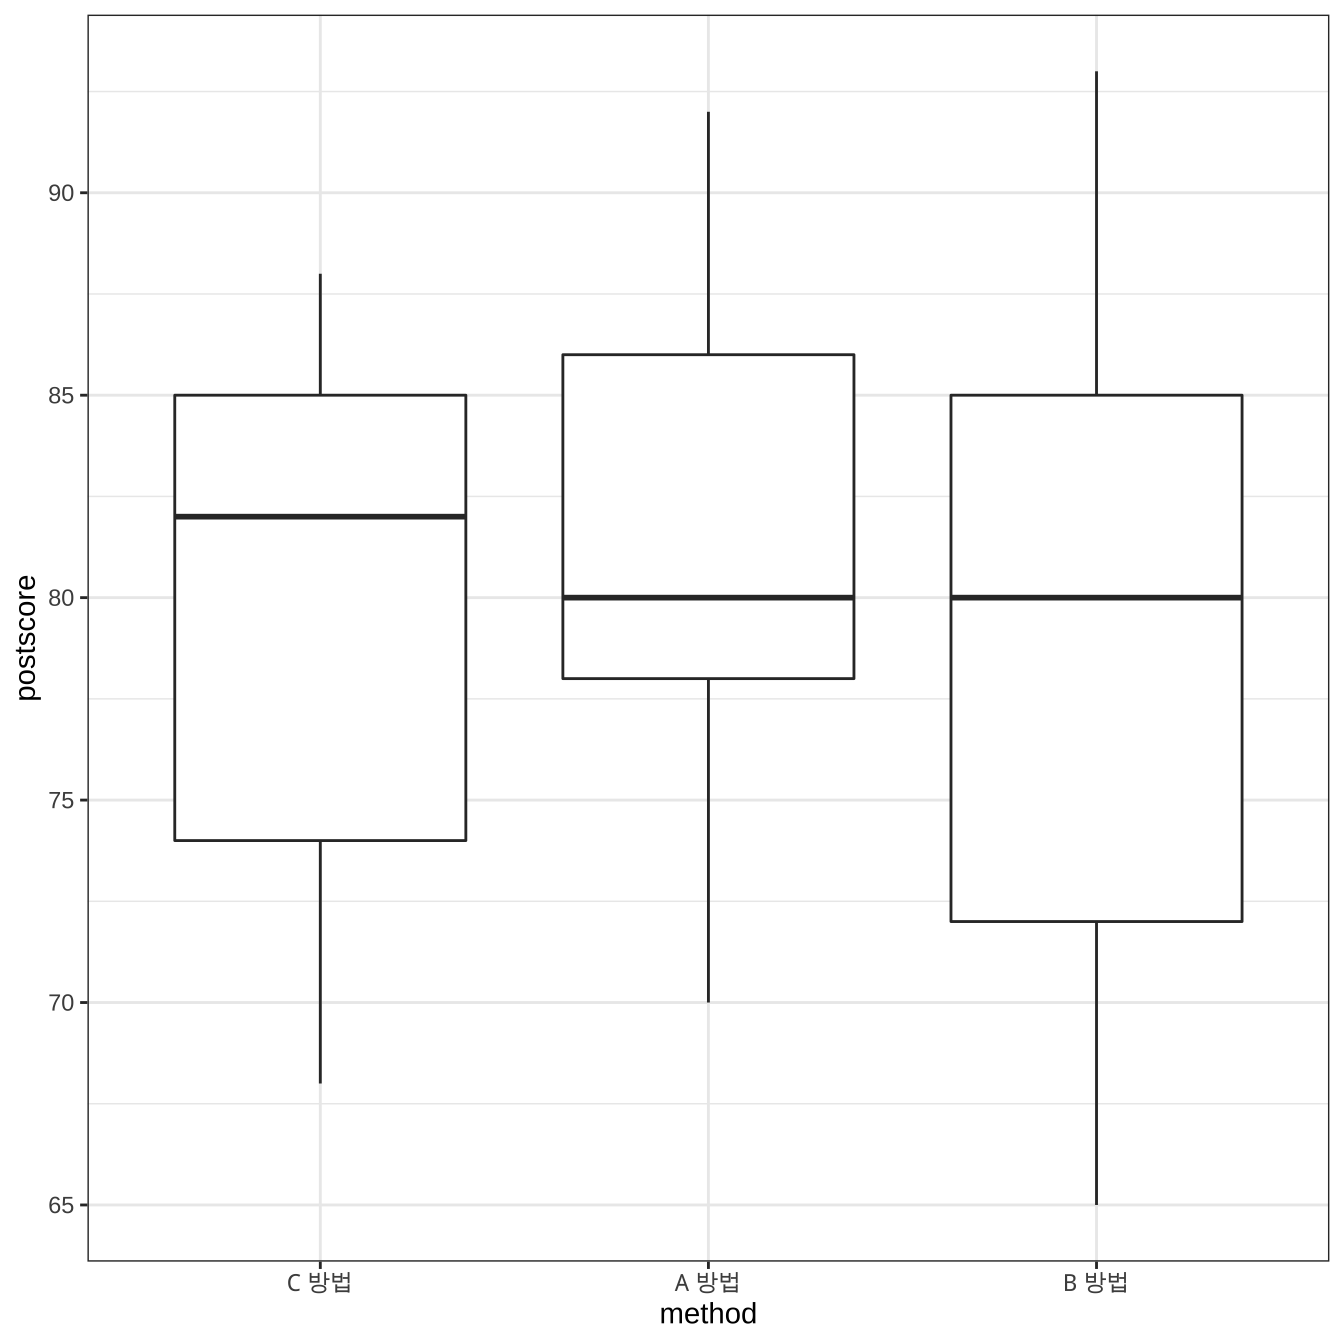
\includegraphics[width=0.7\linewidth]{lmpractice_files/figure-latex/unnamed-chunk-95-1} 

}

\caption{교육방법에 따른 영어 성적}\label{fig:unnamed-chunk-95}
\end{figure}

이제 3가지 교육 방법에 대한 일원배치 분석을 해보자.

\begin{Shaded}
\begin{Highlighting}[]
\NormalTok{fit40 }\OtherTok{\textless{}{-}} \FunctionTok{lm}\NormalTok{(postscore }\SpecialCharTok{\textasciitilde{}}\NormalTok{ method , }\AttributeTok{data=}\NormalTok{english2)}
\FunctionTok{summary}\NormalTok{(fit40)}
\end{Highlighting}
\end{Shaded}

\begin{verbatim}
## 
## Call:
## lm(formula = postscore ~ method, data = english2)
## 
## Residuals:
##     Min      1Q  Median      3Q     Max 
## -14.000  -6.444   1.111   5.556  14.000 
## 
## Coefficients:
##              Estimate Std. Error t value Pr(>|t|)    
## (Intercept)   79.8889     2.7181  29.392   <2e-16 ***
## methodA 방법   1.0000     3.8439   0.260    0.797    
## methodB 방법  -0.8889     3.8439  -0.231    0.819    
## ---
## Signif. codes:  0 '***' 0.001 '**' 0.01 '*' 0.05 '.' 0.1 ' ' 1
## 
## Residual standard error: 8.154 on 24 degrees of freedom
## Multiple R-squared:  0.009972,   Adjusted R-squared:  -0.07253 
## F-statistic: 0.1209 on 2 and 24 DF,  p-value: 0.8867
\end{verbatim}

\begin{Shaded}
\begin{Highlighting}[]
\FunctionTok{anova}\NormalTok{(fit40)}
\end{Highlighting}
\end{Shaded}

\begin{verbatim}
## Analysis of Variance Table
## 
## Response: postscore
##           Df  Sum Sq Mean Sq F value Pr(>F)
## method     2   16.07   8.037  0.1209 0.8867
## Residuals 24 1595.78  66.491
\end{verbatim}

이러한 실험에서 중요한 관심은 세 가지 영어교육 방법의 효과에 차이가 있는 지를 보는 것이지만 학생들의 영어에 대한 선행 능력도 교육의 효과에 영향을 미친다. 이러한 경우
교육 전의 점수 \texttt{prescore}를 공변량(covariate)라고 하며 집단간의 차이를 알아보는 실험에서 반응값에 영향을 미칠 수 있는 여러 가지 공변량을 모형에 같이 포함시키는 방법을 공분산분석(ANCOVA; Analysis of Covariance)라고 한다.

\begin{Shaded}
\begin{Highlighting}[]
\NormalTok{english2 }\SpecialCharTok{\%\textgreater{}\%} \FunctionTok{ggplot}\NormalTok{( }\FunctionTok{aes}\NormalTok{(prescore, postscore)) }\SpecialCharTok{+} \FunctionTok{geom\_point}\NormalTok{(}\FunctionTok{aes}\NormalTok{(}\AttributeTok{colour =}\NormalTok{ method)) }\SpecialCharTok{+} \FunctionTok{theme\_bw}\NormalTok{()}
\end{Highlighting}
\end{Shaded}

\begin{figure}

{\centering 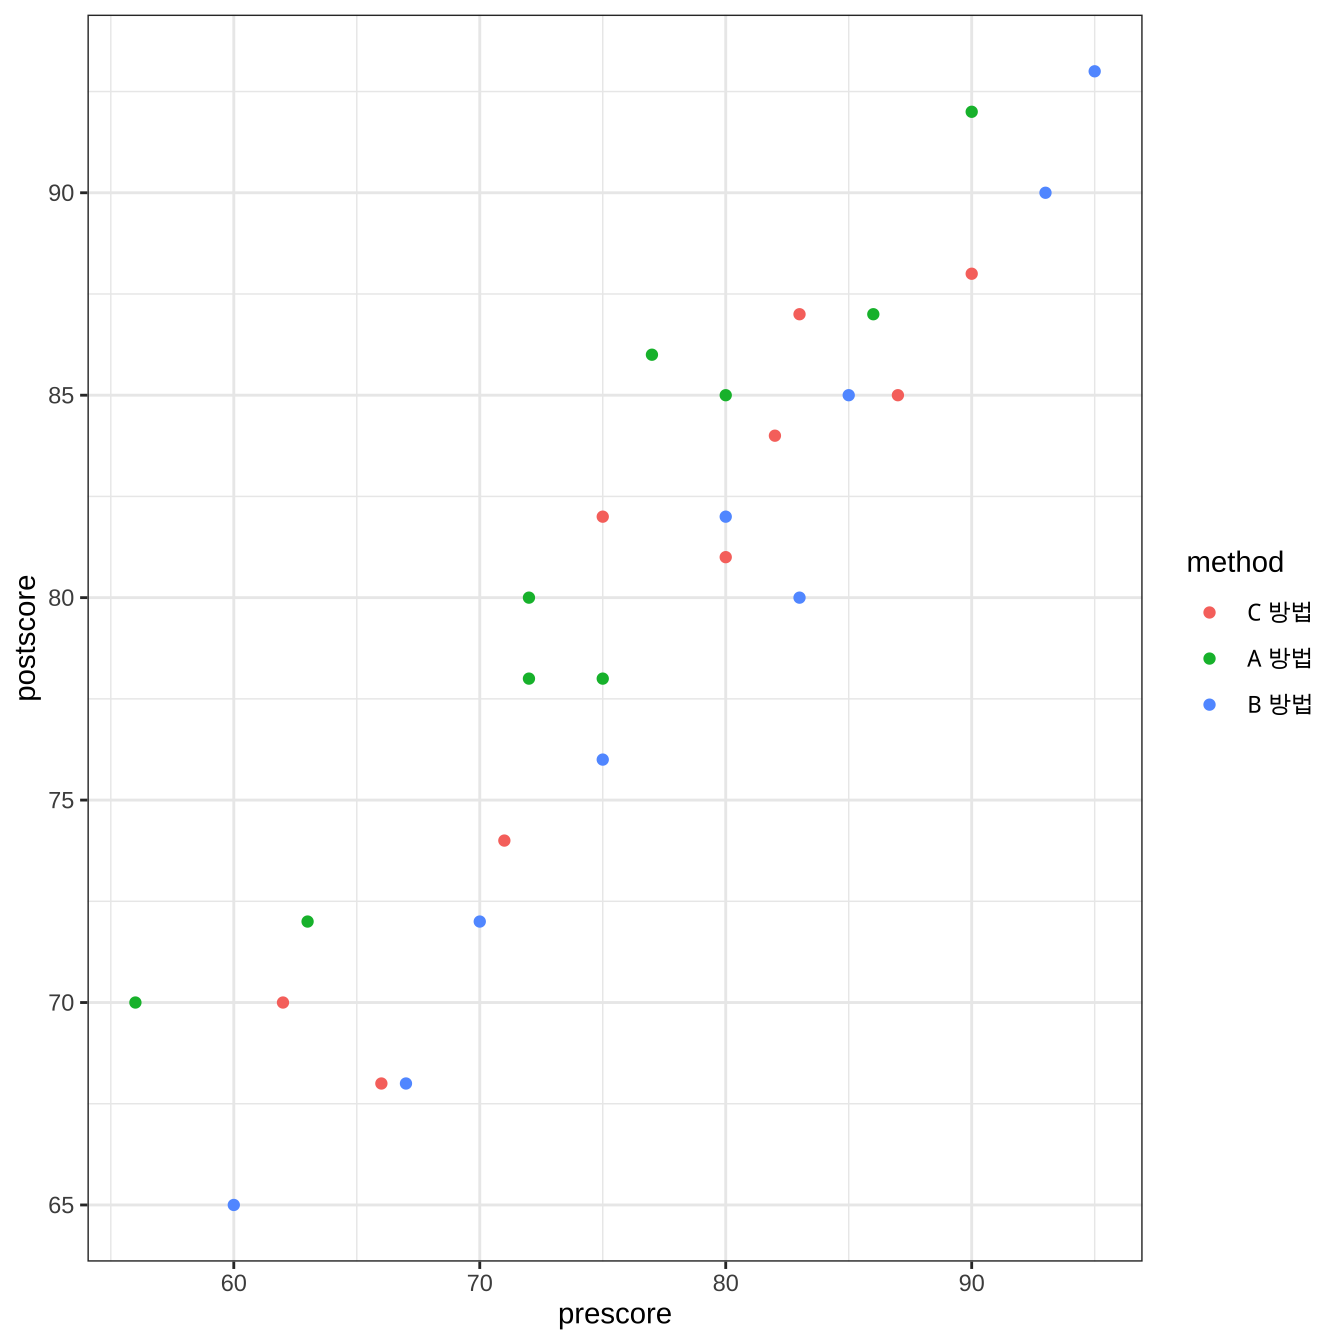
\includegraphics[width=0.7\linewidth]{lmpractice_files/figure-latex/unnamed-chunk-97-1} 

}

\caption{교육 전과 후의 영어 성적}\label{fig:unnamed-chunk-97}
\end{figure}

\begin{Shaded}
\begin{Highlighting}[]
\NormalTok{fit4 }\OtherTok{\textless{}{-}} \FunctionTok{lm}\NormalTok{(postscore }\SpecialCharTok{\textasciitilde{}}\NormalTok{ method }\SpecialCharTok{+}\NormalTok{ prescore, }\AttributeTok{data=}\NormalTok{english2)}
\FunctionTok{summary}\NormalTok{(fit4)}
\end{Highlighting}
\end{Shaded}

\begin{verbatim}
## 
## Call:
## lm(formula = postscore ~ method + prescore, data = english2)
## 
## Residuals:
##     Min      1Q  Median      3Q     Max 
## -3.5044 -1.2316 -0.2874  1.3847  3.8373 
## 
## Coefficients:
##              Estimate Std. Error t value Pr(>|t|)    
## (Intercept)  22.67685    3.22300   7.036 3.61e-07 ***
## methodA 방법  3.05503    1.00713   3.033  0.00591 ** 
## methodB 방법 -1.87530    1.00225  -1.871  0.07411 .  
## prescore      0.73981    0.04066  18.195 3.76e-15 ***
## ---
## Signif. codes:  0 '***' 0.001 '**' 0.01 '*' 0.05 '.' 0.1 ' ' 1
## 
## Residual standard error: 2.123 on 23 degrees of freedom
## Multiple R-squared:  0.9357, Adjusted R-squared:  0.9273 
## F-statistic: 111.5 on 3 and 23 DF,  p-value: 7.563e-14
\end{verbatim}

\begin{Shaded}
\begin{Highlighting}[]
\FunctionTok{anova}\NormalTok{(fit4)}
\end{Highlighting}
\end{Shaded}

\begin{verbatim}
## Analysis of Variance Table
## 
## Response: postscore
##           Df  Sum Sq Mean Sq  F value   Pr(>F)    
## method     2   16.07    8.04   1.7832   0.1906    
## prescore   1 1492.12 1492.12 331.0651 3.76e-15 ***
## Residuals 23  103.66    4.51                      
## ---
## Signif. codes:  0 '***' 0.001 '**' 0.01 '*' 0.05 '.' 0.1 ' ' 1
\end{verbatim}

\hypertarget{uxc608uxc81c-uxacf5uxbd84uxc0b0uxbd84uxc11d-2}{%
\section{예제: 공분산분석 2}\label{uxc608uxc81c-uxacf5uxbd84uxc0b0uxbd84uxc11d-2}}

\begin{rmdwarning}
여기에서 논의되는 예제는 실제 자료가 아닌 인공적인 자료이며 분산분석과 공분산분석을 비교 설명하기 위해서 만든 예제입니다.
\end{rmdwarning}

면역세포의 양을 증가시켜주는 새로운 약의 효과를 측정하기 위하여 한 집단에는 새로운 약(집단 A)를 투여하고 다른 집단에는 위약(집단 P)를 투여하여4주가 지난 후 면역세포가 증가한 비율(percentage; \(y\))를 측정하였다. 즉정된 자료는 다음과 같다.

\begin{Shaded}
\begin{Highlighting}[]
\NormalTok{data1}
\end{Highlighting}
\end{Shaded}

\begin{verbatim}
##    trt        y age
## 1    P 8.814752  25
## 2    P 8.052182  37
## 3    P 8.866027  22
## 4    P 8.120308  33
## 5    P 8.368265  31
## 6    P 8.500431  30
## 7    P 8.410057  29
## 8    P 8.286201  30
## 9    P 8.381821  31
## 10   P 8.523312  28
## 11   P 8.290160  34
## 12   P 8.194626  37
## 13   P 8.830524  22
## 14   P 8.306876  31
## 15   P 8.756627  25
## 16   P 8.380687  32
## 17   P 8.252787  32
## 18   P 8.736798  23
## 19   P 8.256965  32
## 20   P 8.652589  32
## 21   A 8.099116  48
## 22   A 7.505564  65
## 23   A 8.872682  36
## 24   A 8.040548  49
## 25   A 8.465196  45
## 26   A 8.350292  48
## 27   A 8.277757  48
## 28   A 8.366004  46
## 29   A 8.195370  49
## 30   A 7.774903  53
## 31   A 8.305913  47
## 32   A 8.442647  47
## 33   A 8.246845  49
## 34   A 8.452886  51
## 35   A 8.710324  47
## 36   A 8.311612  46
## 37   A 7.798335  57
## 38   A 8.688703  44
## 39   A 8.181481  49
## 40   A 8.086845  47
\end{verbatim}

이제 두 처리 집단의 반응값을 비교해 보자.

\begin{Shaded}
\begin{Highlighting}[]
\NormalTok{data1 }\SpecialCharTok{\%\textgreater{}\%} \FunctionTok{ggplot}\NormalTok{(}\FunctionTok{aes}\NormalTok{(trt, y)) }\SpecialCharTok{+} \FunctionTok{geom\_boxplot}\NormalTok{()  }\SpecialCharTok{+} \FunctionTok{theme\_bw}\NormalTok{()}
\end{Highlighting}
\end{Shaded}

\begin{figure}

{\centering 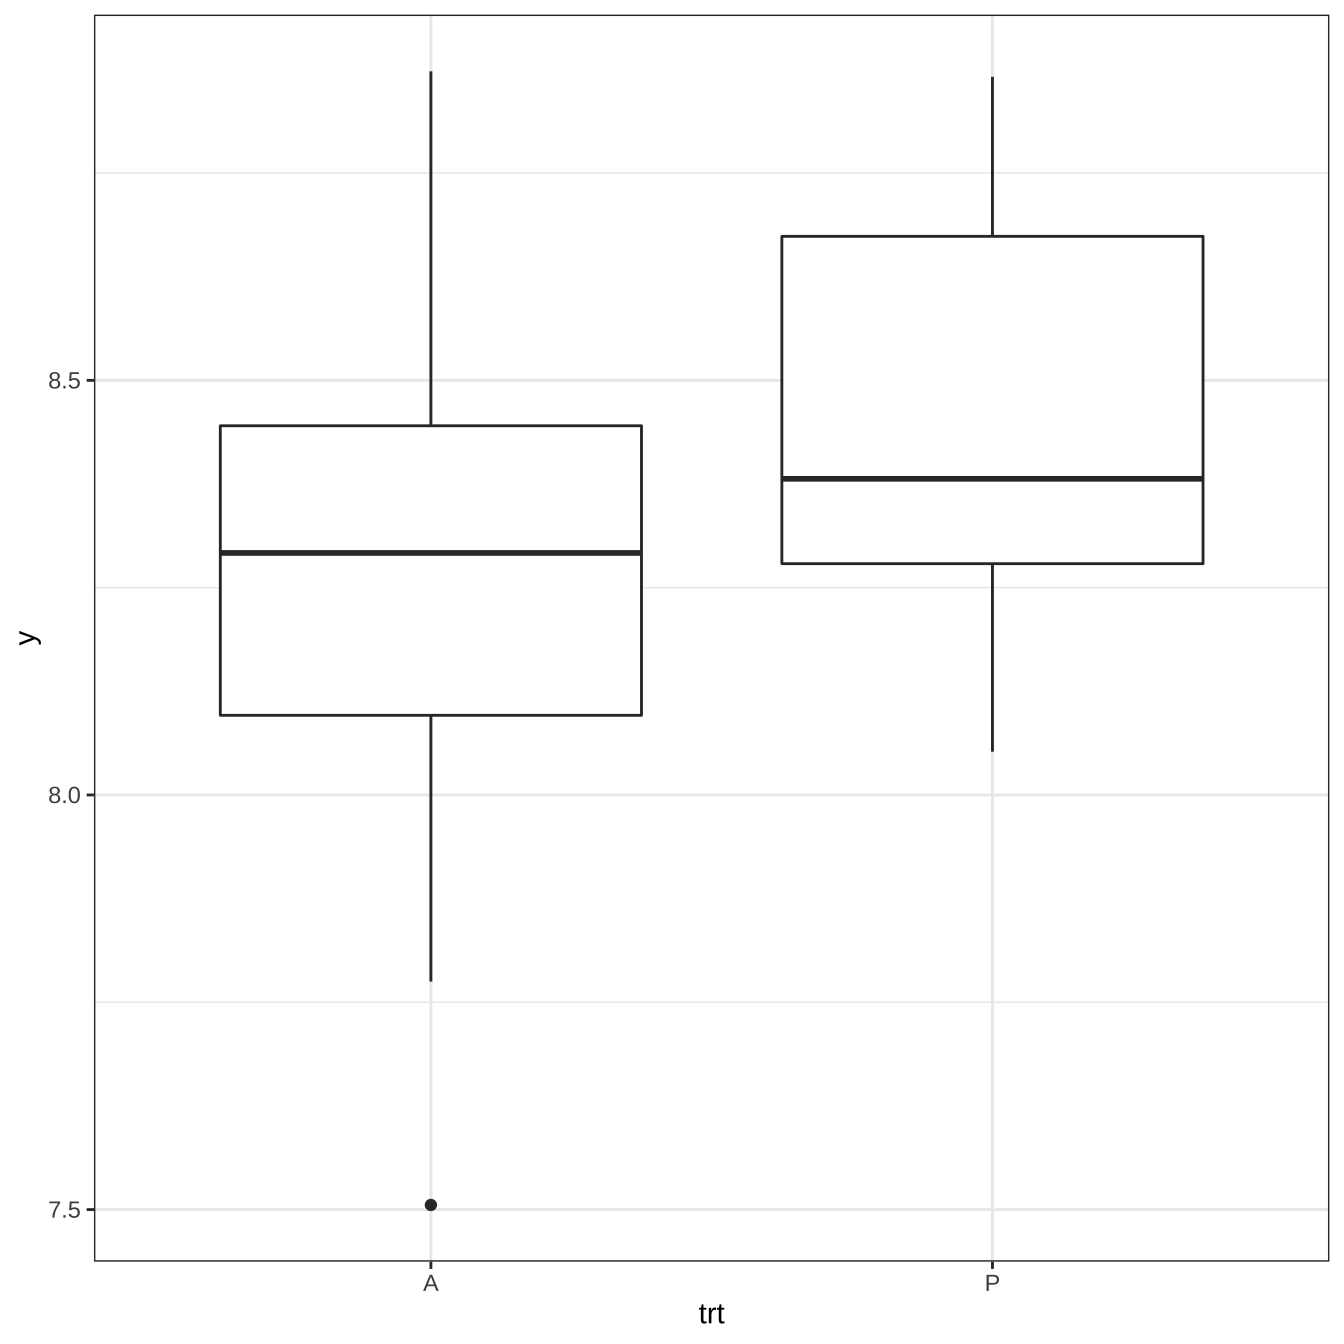
\includegraphics[width=0.7\linewidth]{lmpractice_files/figure-latex/unnamed-chunk-102-1} 

}

\caption{처리 집단에 따른 반응값}\label{fig:unnamed-chunk-102}
\end{figure}

위의 그림에서 나타난 것과 같이 위약를 투여한 집단 P의 면역세포 증가비율이 새로운 약을 투여한 집단 A보다 평균적으로 크다는 것을 알 수 있다.

따라서 약을 복용하지 않는 것이 면역세포를 증가시키는데 도움이 된다는 비상식적인 결론이 분석에서 얻어진것이다.

일원배치 분산분석 모형에서 두 집단의 평균의 차이가 있는지 대한 가설을 검정할 수 있다.

\begin{Shaded}
\begin{Highlighting}[]
\NormalTok{anova.fit }\OtherTok{\textless{}{-}} \FunctionTok{lm}\NormalTok{(y}\SpecialCharTok{\textasciitilde{}}\NormalTok{trt,}\AttributeTok{data=}\NormalTok{data1)}
\FunctionTok{summary}\NormalTok{(anova.fit)}
\end{Highlighting}
\end{Shaded}

\begin{verbatim}
## 
## Call:
## lm(formula = y ~ trt, data = data1)
## 
## Residuals:
##      Min       1Q   Median       3Q      Max 
## -0.75309 -0.16513 -0.02542  0.19655  0.61403 
## 
## Coefficients:
##             Estimate Std. Error t value Pr(>|t|)    
## (Intercept)  8.25865    0.06495 127.149   <2e-16 ***
## trtP         0.19045    0.09186   2.073    0.045 *  
## ---
## Signif. codes:  0 '***' 0.001 '**' 0.01 '*' 0.05 '.' 0.1 ' ' 1
## 
## Residual standard error: 0.2905 on 38 degrees of freedom
## Multiple R-squared:  0.1016, Adjusted R-squared:  0.07799 
## F-statistic: 4.299 on 1 and 38 DF,  p-value: 0.04497
\end{verbatim}

\begin{Shaded}
\begin{Highlighting}[]
\FunctionTok{anova}\NormalTok{(anova.fit)}
\end{Highlighting}
\end{Shaded}

\begin{verbatim}
## Analysis of Variance Table
## 
## Response: y
##           Df Sum Sq Mean Sq F value  Pr(>F)  
## trt        1 0.3627 0.36271  4.2987 0.04497 *
## Residuals 38 3.2063 0.08438                  
## ---
## Signif. codes:  0 '***' 0.001 '**' 0.01 '*' 0.05 '.' 0.1 ' ' 1
\end{verbatim}

두 집단을 ANOVA를 이용한 F 검정으로 비교해 보면 p-값이 0.045로서
두 집단간의 유의한 차이가 있음을 알 수 있으며 이 유의한 차이는 위약를 투여한 집단 P의 면역새포 증가 비율 집단 A보다 크다는 것을 의미한다.

그런데 두 집단에 속한 환자들의 연령를 비교해 보면 위약를 투여한 집단 P의 평균 나이가 새로운 약을 투여한 집단 A의 평균 나이보다 20세 정도 적다. 따라서 콜레스테롤이 감소한 결과가 약효의 차이 때문인지 나이의 차이때문인지 확신할 수 없다.

\begin{Shaded}
\begin{Highlighting}[]
\NormalTok{data1 }\SpecialCharTok{\%\textgreater{}\%} \FunctionTok{ggplot}\NormalTok{( }\FunctionTok{aes}\NormalTok{(age, y)) }\SpecialCharTok{+} \FunctionTok{geom\_point}\NormalTok{(}\FunctionTok{aes}\NormalTok{(}\AttributeTok{colour =}\NormalTok{ trt)) }\SpecialCharTok{+} \FunctionTok{theme\_bw}\NormalTok{()}
\end{Highlighting}
\end{Shaded}

\begin{figure}

{\centering 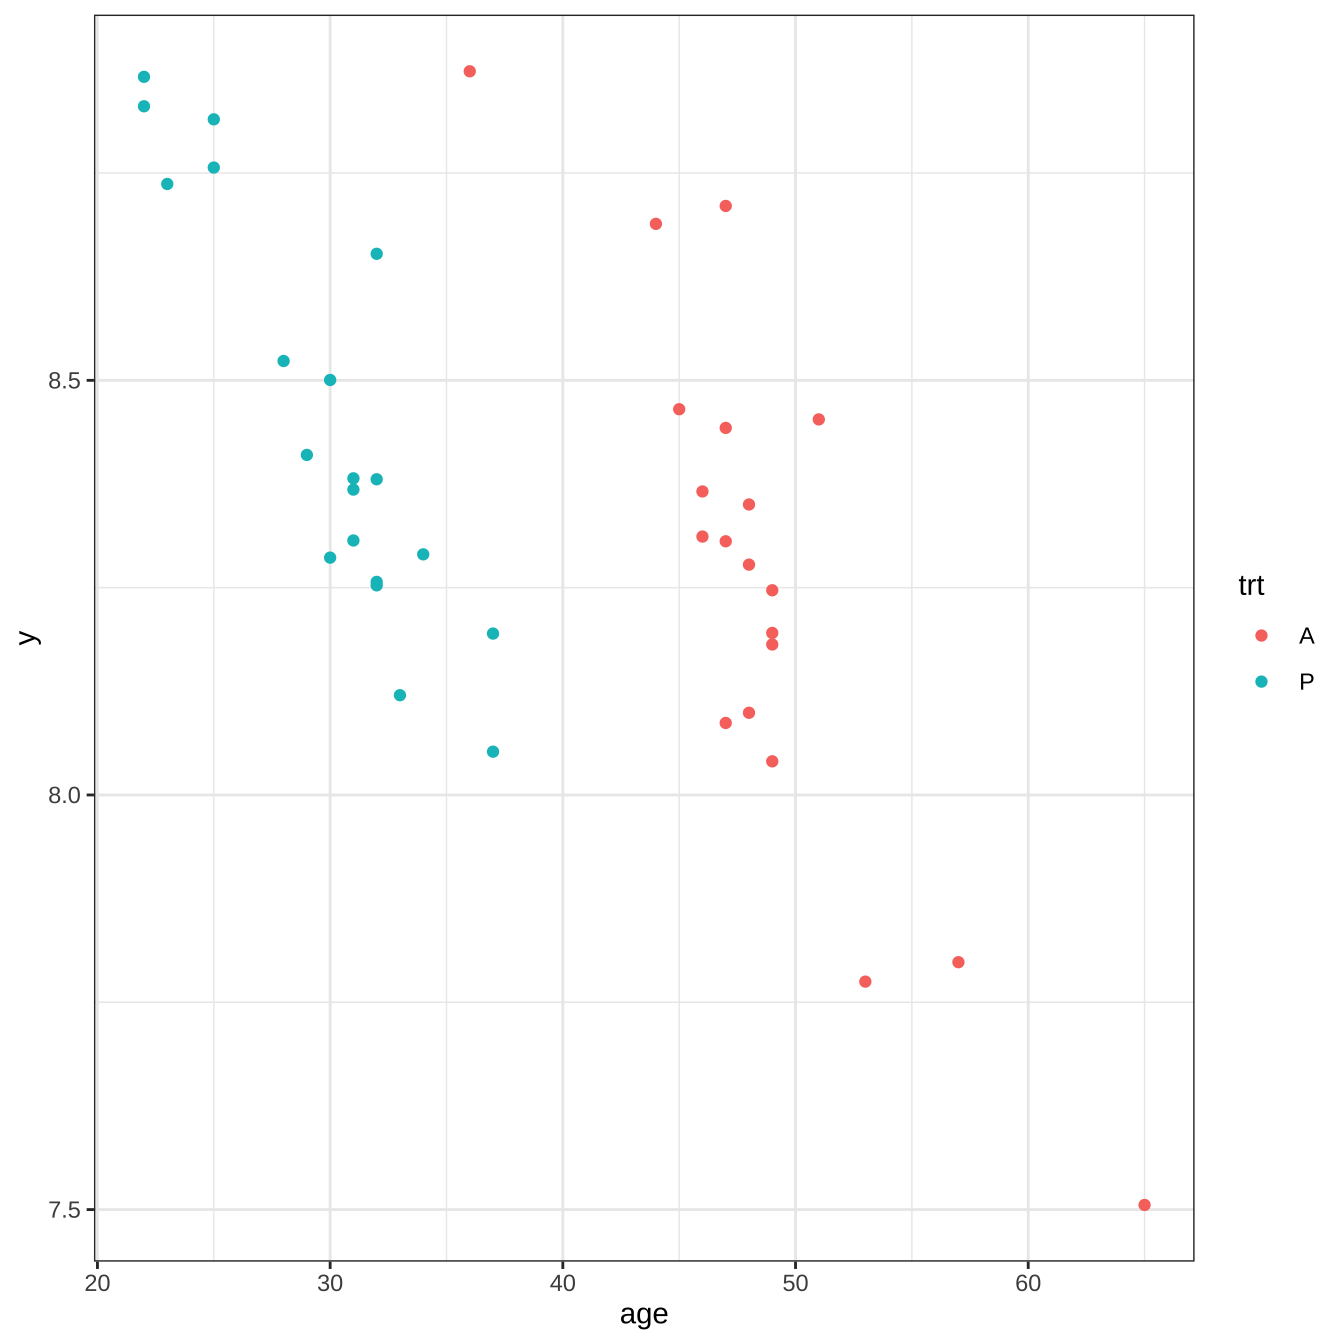
\includegraphics[width=0.9\linewidth]{lmpractice_files/figure-latex/unnamed-chunk-104-1} 

}

\caption{나이와 반응변수의 관계}\label{fig:unnamed-chunk-104}
\end{figure}

\begin{Shaded}
\begin{Highlighting}[]
\NormalTok{data1sum }\OtherTok{\textless{}{-}}\NormalTok{data1 }\SpecialCharTok{\%\textgreater{}\%} \FunctionTok{group\_by}\NormalTok{(trt)  }\SpecialCharTok{\%\textgreater{}\%}  \FunctionTok{summarise}\NormalTok{(}\AttributeTok{mean=}\FunctionTok{mean}\NormalTok{(age), }\AttributeTok{median=} \FunctionTok{median}\NormalTok{(age), }\AttributeTok{sd=}\FunctionTok{sd}\NormalTok{(age), }\AttributeTok{min=}\FunctionTok{min}\NormalTok{(age), }\AttributeTok{max=}\FunctionTok{max}\NormalTok{(age))}
\NormalTok{data1sum }
\end{Highlighting}
\end{Shaded}

\begin{verbatim}
## # A tibble: 2 x 6
##   trt    mean median    sd   min   max
##   <fct> <dbl>  <dbl> <dbl> <dbl> <dbl>
## 1 A      48.6     48  5.54    36    65
## 2 P      29.8     31  4.43    22    37
\end{verbatim}

따라서 연령을 공변량으로 반영하여 공분산 분석을 적용하기로 하였다.

\begin{Shaded}
\begin{Highlighting}[]
\NormalTok{ancova.fit }\OtherTok{\textless{}{-}} \FunctionTok{lm}\NormalTok{(y}\SpecialCharTok{\textasciitilde{}}\NormalTok{trt}\SpecialCharTok{+}\NormalTok{age,}\AttributeTok{data=}\NormalTok{data1)}
\FunctionTok{summary}\NormalTok{(ancova.fit)}
\end{Highlighting}
\end{Shaded}

\begin{verbatim}
## 
## Call:
## lm(formula = y ~ trt + age, data = data1)
## 
## Residuals:
##      Min       1Q   Median       3Q      Max 
## -0.25781 -0.07730 -0.01854  0.06204  0.37297 
## 
## Coefficients:
##              Estimate Std. Error t value Pr(>|t|)    
## (Intercept) 10.723681   0.224503  47.766  < 2e-16 ***
## trtP        -0.761545   0.096808  -7.867 2.05e-09 ***
## age         -0.050773   0.004578 -11.091 2.54e-13 ***
## ---
## Signif. codes:  0 '***' 0.001 '**' 0.01 '*' 0.05 '.' 0.1 ' ' 1
## 
## Residual standard error: 0.1416 on 37 degrees of freedom
## Multiple R-squared:  0.7923, Adjusted R-squared:  0.781 
## F-statistic: 70.55 on 2 and 37 DF,  p-value: 2.367e-13
\end{verbatim}

\begin{Shaded}
\begin{Highlighting}[]
\FunctionTok{anova}\NormalTok{(ancova.fit)}
\end{Highlighting}
\end{Shaded}

\begin{verbatim}
## Analysis of Variance Table
## 
## Response: y
##           Df  Sum Sq Mean Sq F value    Pr(>F)    
## trt        1 0.36271 0.36271    18.1  0.000137 ***
## age        1 2.46486 2.46486   123.0 2.535e-13 ***
## Residuals 37 0.74144 0.02004                      
## ---
## Signif. codes:  0 '***' 0.001 '**' 0.01 '*' 0.05 '.' 0.1 ' ' 1
\end{verbatim}

공분산 분석의 결과를 보면 집단 P에 대한 계수가 \(trtP= -0.761545\)로 집단 A보다 평균적으로 \(0.76\) 낮다는 것을 알수 있다.

\begin{center}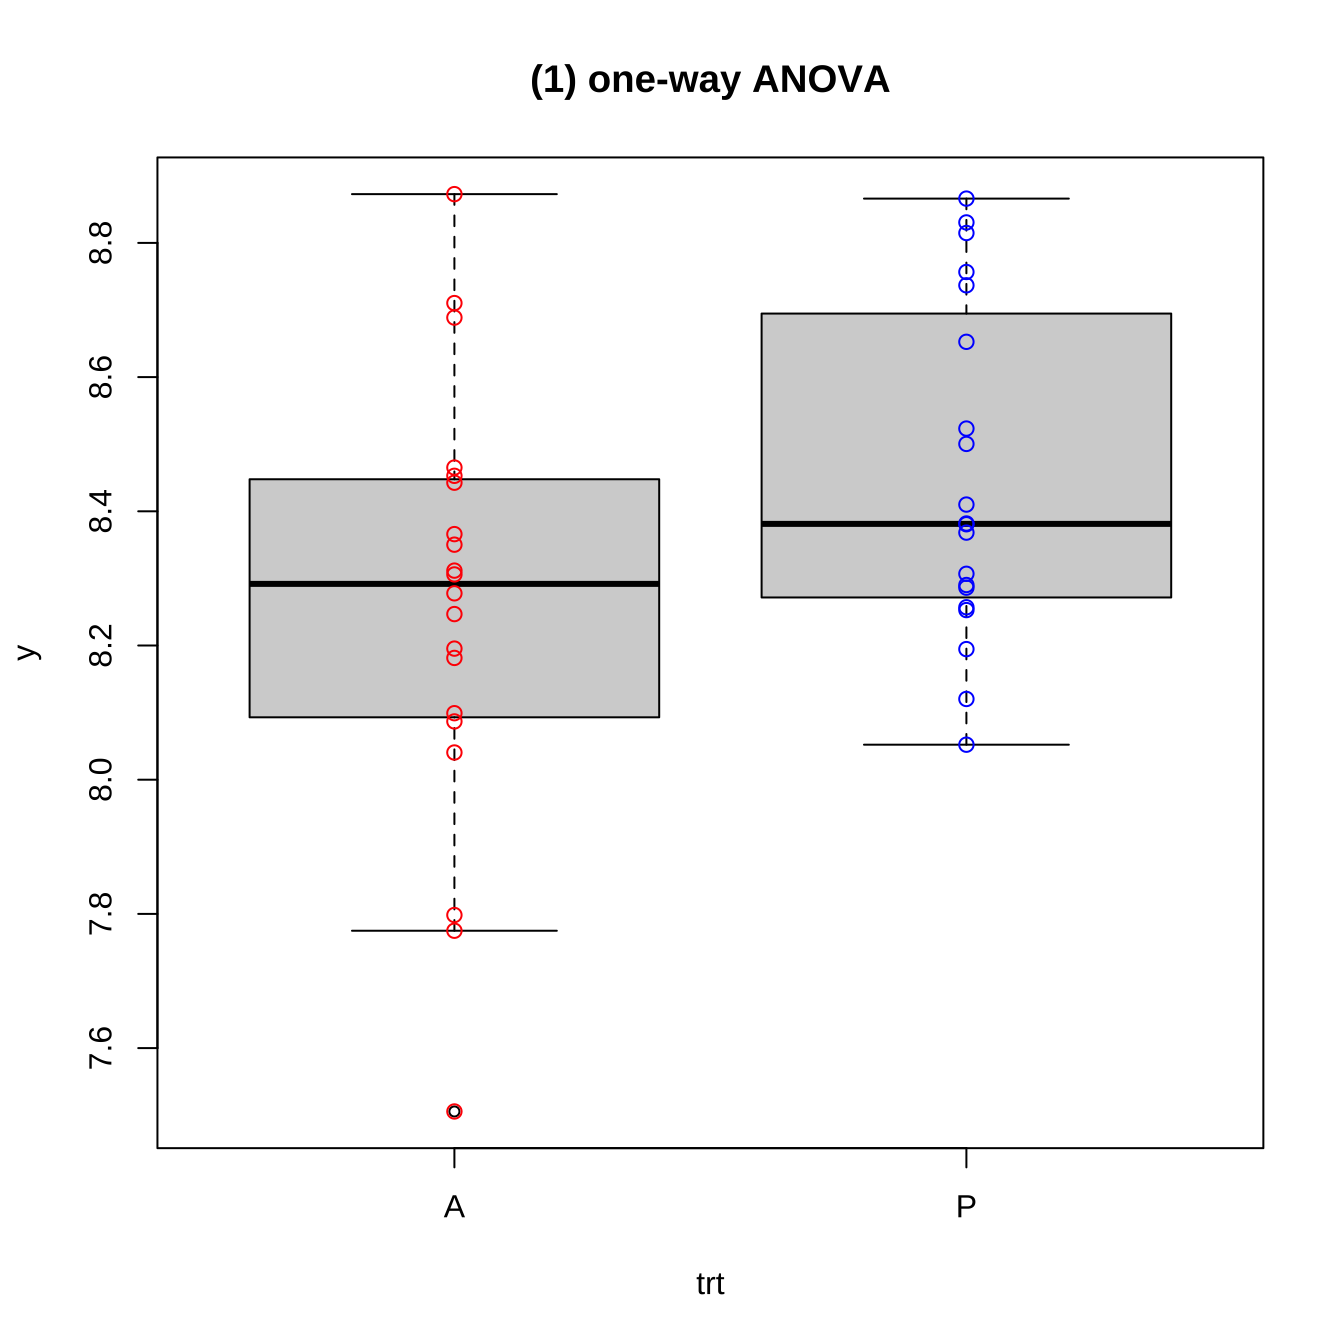
\includegraphics[width=0.6\linewidth]{lmpractice_files/figure-latex/unnamed-chunk-107-1} 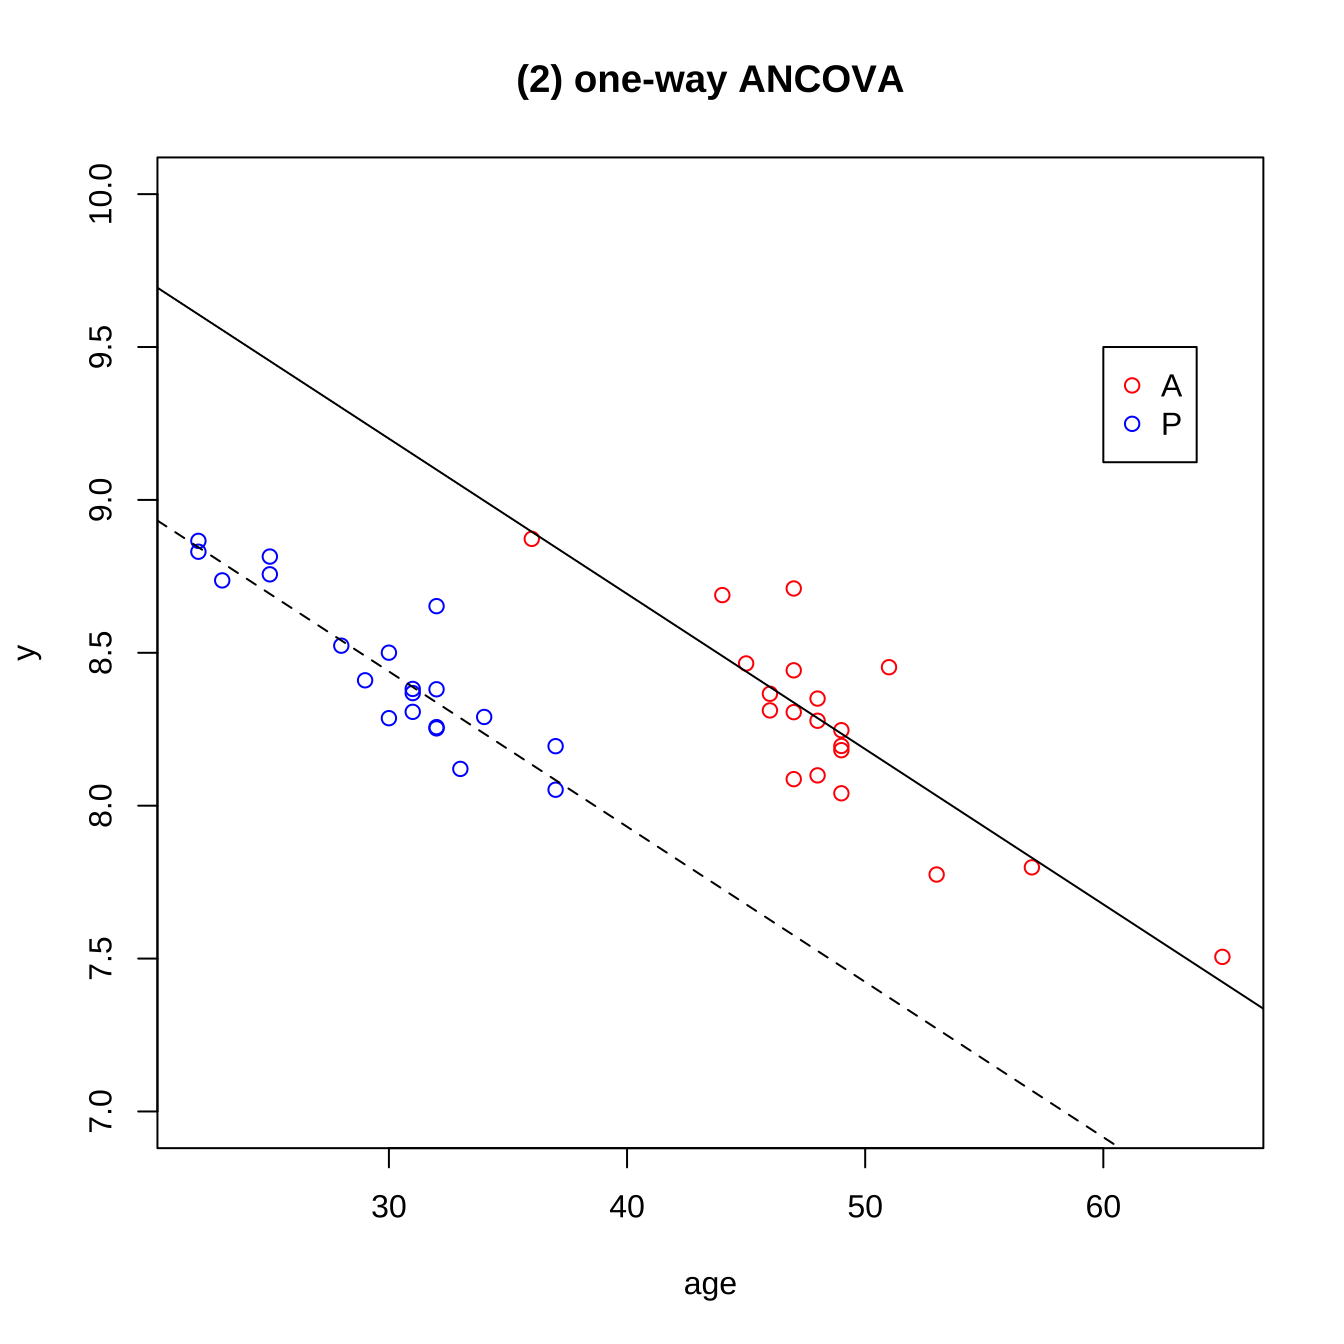
\includegraphics[width=0.6\linewidth]{lmpractice_files/figure-latex/unnamed-chunk-107-2} \end{center}

위의 그림에서 나타난 바와 같이 연령의 효과를 반영하면 집단 A의 회귀식이 집단 P의
회귀식보다 위에 위치함을 알 수 있고 이는 집단 A의 회귀식의 절편이 집단 P의 회귀식의 절편보다 크다는 것을 의미하며 이는 새로운 약을 투여한 집단의 면역세포 증가 비율이 위약 집단보다 크다는 것을 의미한다.

또한 연령에 대한 기울기를 보면 \(-0.050669\)으로서
나이가 많을 수록 면역세포 증가 비율이 작아짐을 알 수 있다.

따라서 나이를 고려하지 않은 일원배치 분산분석에서
두 집단의 차이는 20세라는 평균 나이에 의한 차이 즉, \((20) \times (-0.050669)= -1.01\)과 약의 효과에 의한 차이가 상호작용하여 비상식적인 결과가 나타난 것이다.

한가지 더 주목할 점은 나이를 고려하지 않은 일원배치 분산분석에서 오차항의 분산에 대한 추정량은
\(\hat \sigma^2 = (0.2916)^2 =0.085\)이며 공분산 분석에서는 \(\hat \sigma^2 = (0.1416)^2 =0.020\)으로
줄어 들었다. 이는 공분산 분석이 자료의 변동 중 처리(treament)로 설명할 수 없는 부분을 공변량인 나이를 이용하여 부가적으로 설명해준다 것을 알수 있다.

\hypertarget{uxc5f0uxc2b5uxbb38uxc81c-7.13}{%
\section{연습문제 7.13}\label{uxc5f0uxc2b5uxbb38uxc81c-7.13}}

\begin{Shaded}
\begin{Highlighting}[]
\NormalTok{fit5 }\OtherTok{\textless{}{-}} \FunctionTok{lm}\NormalTok{(postscore }\SpecialCharTok{\textasciitilde{}}\NormalTok{ method , }\AttributeTok{data=}\NormalTok{english2)}
\FunctionTok{summary}\NormalTok{(fit5)}
\end{Highlighting}
\end{Shaded}

\begin{verbatim}
## 
## Call:
## lm(formula = postscore ~ method, data = english2)
## 
## Residuals:
##     Min      1Q  Median      3Q     Max 
## -14.000  -6.444   1.111   5.556  14.000 
## 
## Coefficients:
##              Estimate Std. Error t value Pr(>|t|)    
## (Intercept)   79.8889     2.7181  29.392   <2e-16 ***
## methodA 방법   1.0000     3.8439   0.260    0.797    
## methodB 방법  -0.8889     3.8439  -0.231    0.819    
## ---
## Signif. codes:  0 '***' 0.001 '**' 0.01 '*' 0.05 '.' 0.1 ' ' 1
## 
## Residual standard error: 8.154 on 24 degrees of freedom
## Multiple R-squared:  0.009972,   Adjusted R-squared:  -0.07253 
## F-statistic: 0.1209 on 2 and 24 DF,  p-value: 0.8867
\end{verbatim}

\begin{Shaded}
\begin{Highlighting}[]
\FunctionTok{anova}\NormalTok{(fit5)}
\end{Highlighting}
\end{Shaded}

\begin{verbatim}
## Analysis of Variance Table
## 
## Response: postscore
##           Df  Sum Sq Mean Sq F value Pr(>F)
## method     2   16.07   8.037  0.1209 0.8867
## Residuals 24 1595.78  66.491
\end{verbatim}

\begin{Shaded}
\begin{Highlighting}[]
\NormalTok{fit6 }\OtherTok{\textless{}{-}} \FunctionTok{lm}\NormalTok{(postscore }\SpecialCharTok{\textasciitilde{}}\NormalTok{ method }\SpecialCharTok{+}\NormalTok{ prescore }\SpecialCharTok{+}\NormalTok{ method}\SpecialCharTok{:}\NormalTok{prescore , }\AttributeTok{data=}\NormalTok{english2)}
\FunctionTok{summary}\NormalTok{(fit6)}
\end{Highlighting}
\end{Shaded}

\begin{verbatim}
## 
## Call:
## lm(formula = postscore ~ method + prescore + method:prescore, 
##     data = english2)
## 
## Residuals:
##     Min      1Q  Median      3Q     Max 
## -3.5402 -1.2554  0.0054  1.0200  3.8300 
## 
## Coefficients:
##                       Estimate Std. Error t value Pr(>|t|)    
## (Intercept)           22.92142    6.07039   3.776  0.00111 ** 
## methodA 방법           8.92311    8.03989   1.110  0.27961    
## methodB 방법          -7.50913    7.87202  -0.954  0.35099    
## prescore               0.73665    0.07797   9.447 5.19e-09 ***
## methodA 방법:prescore -0.07883    0.10484  -0.752  0.46048    
## methodB 방법:prescore  0.07167    0.10030   0.715  0.48275    
## ---
## Signif. codes:  0 '***' 0.001 '**' 0.01 '*' 0.05 '.' 0.1 ' ' 1
## 
## Residual standard error: 2.098 on 21 degrees of freedom
## Multiple R-squared:  0.9427, Adjusted R-squared:  0.929 
## F-statistic: 69.04 on 5 and 21 DF,  p-value: 2.575e-12
\end{verbatim}

\begin{Shaded}
\begin{Highlighting}[]
\FunctionTok{anova}\NormalTok{(fit6)}
\end{Highlighting}
\end{Shaded}

\begin{verbatim}
## Analysis of Variance Table
## 
## Response: postscore
##                 Df  Sum Sq Mean Sq  F value   Pr(>F)    
## method           2   16.07    8.04   1.8258   0.1857    
## prescore         1 1492.12 1492.12 338.9743 1.95e-14 ***
## method:prescore  2   11.22    5.61   1.2747   0.3003    
## Residuals       21   92.44    4.40                      
## ---
## Signif. codes:  0 '***' 0.001 '**' 0.01 '*' 0.05 '.' 0.1 ' ' 1
\end{verbatim}

\hypertarget{chapter06}{%
\chapter{회귀모형의 선택}\label{chapter06}}

\hypertarget{uxbcc0uxc218uxc120uxd0dduxc758-uxae30uxc900}{%
\section{변수선택의 기준}\label{uxbcc0uxc218uxc120uxd0dduxc758-uxae30uxc900}}

패키지 \texttt{leap} 에 수록된 \texttt{regsubsets()} 함수를 이용하면 가능한 모든 모형에 대한 중요한 선택 기준들이
게산된다.

\begin{itemize}
\tightlist
\item
  `rss``: 잔차 제곱합
\item
  \texttt{rsq}: \(R^2\)
\item
  \texttt{adjr2} : 수정된 \(R^2\)
\item
  \texttt{cp} : 맬로우의 \(C_p\)
\item
  \texttt{bic} : BIC
\end{itemize}

교재 예제에 나타난 자료 \texttt{houseprice}는 독립변수의 수가 4개이므로 가능한 회귀식의 개수가 \(2^4=16\)개이므로 이러한 방법을 적용할 수 있다. 하지만 독립변수의 수가 10개만 되고 가능한 회귀식의 수가 1024개나 되고 20개가 모형의 수가 100만개가 넘으므로 이들 모두에 대한 통계량을 계산하는 것은 실제로 쉽지않다.

이제 예제 자료 \texttt{houseprice}에 대하여 \texttt{regsubsets}함수를 사용하여 가능한 회귀식을 모두 적합하고 각 식에 대한 모형선택의 기준값을 계산해보자. \texttt{regsubsets}함수에서 \texttt{nbest=6}는 독립변수의 수가 같은 모형들 중에서 가장 좋은 6개의 모형만을 보여주라는 명령문이다.

모든 가능한 회귀식에 대한 통계량은 \texttt{summaryf}함수를 통하여 볼 수 있다.

\begin{Shaded}
\begin{Highlighting}[]
\NormalTok{houseprice.rgs }\OtherTok{\textless{}{-}} \FunctionTok{regsubsets}\NormalTok{(price }\SpecialCharTok{\textasciitilde{}}\NormalTok{ . , }\AttributeTok{data=}\NormalTok{houseprice, }\AttributeTok{nbest=}\DecValTok{6}\NormalTok{)}
\FunctionTok{summaryf}\NormalTok{(houseprice.rgs)}
\end{Highlighting}
\end{Shaded}

\begin{verbatim}
##          tax ground floor year        rss        rsq      adjr2         cp        bic
## 1  ( 1 )                *       182.66315 0.86271916 0.85722792  20.943616 -47.022941
## 1  ( 2 )   *                    215.97764 0.83768158 0.83118885  28.958146 -42.499601
## 1  ( 3 )          *             628.61671 0.52756188 0.50866435 128.227503 -13.654236
## 1  ( 4 )                     * 1202.47186 0.09627993 0.06013112 266.280912   3.858312
## 2  ( 1 )   *            *        95.19550 0.92845564 0.92249361   1.901360 -61.323304
## 2  ( 2 )                *    *  153.80917 0.88440442 0.87477146  16.002160 -48.369244
## 2  ( 3 )          *     *       168.58785 0.87329747 0.86273892  19.557496 -45.892146
## 2  ( 4 )   *      *             191.93607 0.85575007 0.84372925  25.174420 -42.390102
## 2  ( 5 )   *                 *  214.64151 0.83868576 0.82524290  30.636710 -39.371316
## 2  ( 6 )          *          *  626.80968 0.52891996 0.48966329 129.792782 -10.436125
## 3  ( 1 )   *            *    *   92.31936 0.93061720 0.92156727   3.209442 -58.855794
## 3  ( 2 )   *      *     *        93.26197 0.92990878 0.92076645   3.436208 -58.581513
## 3  ( 3 )          *     *    *  150.10029 0.88719183 0.87247773  17.109908 -45.732450
## 3  ( 4 )   *      *          *  187.51305 0.85907420 0.84069258  26.110366 -39.723741
## 4  ( 1 )   *      *     *    *   91.44876 0.93127151 0.91877542   5.000000 -55.815783
\end{verbatim}

위의 결과를 보면 두 개의 변수 \texttt{tax}와 \texttt{floor}가 포함된 회귀식이 다음과 같은 통계량으로 가장 좋은 모형으로 나타난다.

\begin{itemize}
\tightlist
\item
  \texttt{rss}: 잔차제곱합(residual sum of square), \(SSE = 95.20\)
\item
  \texttt{rsq}: 결정계수(\(R^2_p\)), \(R^2=0.92846\)
\item
  \texttt{adjr2}: 수정된 결정계수(\(R^2_{ap}\)), \(R^2_a=0.92249\)
\item
  \texttt{cp}: 맬로우즈 \(C_p\), \(C_p = 1.901\)
\item
  \texttt{bic}: BIC(Bayesian Information Criteria), \(BIC= -61.323\)
\end{itemize}

다음은 변수들이 포함되어 나타나는 선택된 기준의 값을 그림으로 표시한 것이다.
Y 축은 선택 기준의 값이고 X축은 변수들의 포함 여부을 나타낸다.

\begin{Shaded}
\begin{Highlighting}[]
\FunctionTok{plot}\NormalTok{(houseprice.rgs , }\AttributeTok{scale =} \StringTok{"bic"}\NormalTok{, }\AttributeTok{main =} \StringTok{"BIC"}\NormalTok{)}
\end{Highlighting}
\end{Shaded}

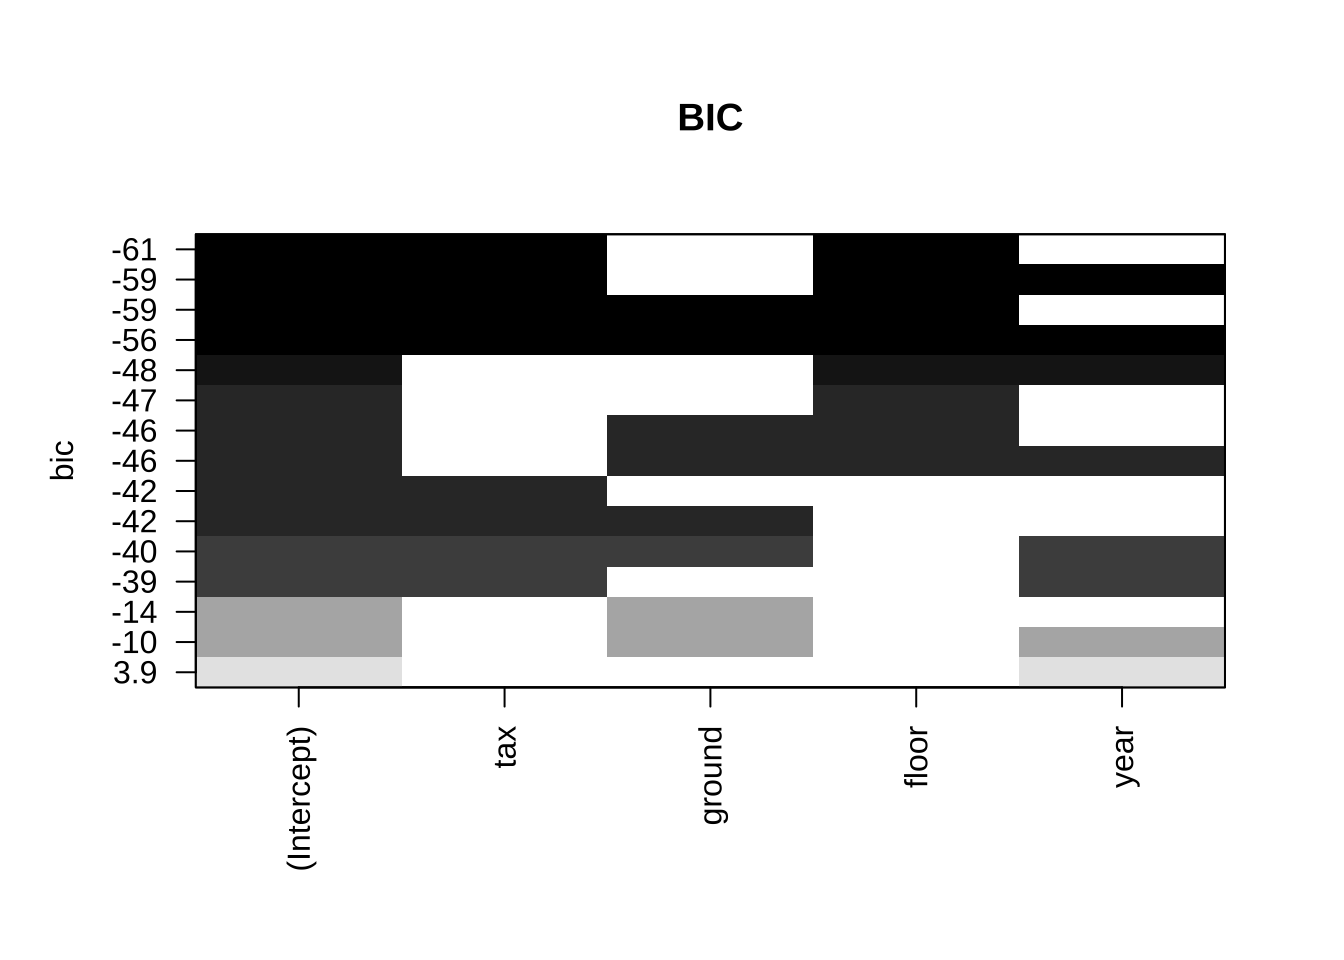
\includegraphics{lmpractice_files/figure-latex/unnamed-chunk-110-1.pdf}
패키지 \texttt{olsrr}에 있는 함수 \texttt{ols\_step\_all\_possible()}을 이용하면 가능한 모등회귀에 대한
통계량을 구하고 여러 가지 통계량에 대한 그림을 \texttt{plot()} 함수를 이용하여 쉽게 그릴 수 있다.

\begin{Shaded}
\begin{Highlighting}[]
\NormalTok{fit1 }\OtherTok{\textless{}{-}} \FunctionTok{lm}\NormalTok{(price }\SpecialCharTok{\textasciitilde{}}\NormalTok{ ., }\AttributeTok{data=}\NormalTok{houseprice)}
\NormalTok{houseprice.rgs2 }\OtherTok{\textless{}{-}} \FunctionTok{ols\_step\_all\_possible}\NormalTok{(fit1)}
\NormalTok{houseprice.rgs2}
\end{Highlighting}
\end{Shaded}

\begin{verbatim}
##    Index N            Predictors   R-Square Adj. R-Square Mallow's Cp
## 3      1 1                 floor 0.86271916    0.85722792   20.943616
## 1      2 1                   tax 0.83768158    0.83118885   28.958146
## 2      3 1                ground 0.52756188    0.50866435  128.227503
## 4      4 1                  year 0.09627993    0.06013112  266.280912
## 6      5 2             tax floor 0.92845564    0.92249361    1.901360
## 10     6 2            floor year 0.88440442    0.87477146   16.002160
## 8      7 2          ground floor 0.87329747    0.86273892   19.557496
## 5      8 2            tax ground 0.85575007    0.84372925   25.174420
## 7      9 2              tax year 0.83868576    0.82524290   30.636710
## 9     10 2           ground year 0.52891996    0.48966329  129.792782
## 13    11 3        tax floor year 0.93061720    0.92156727    3.209442
## 11    12 3      tax ground floor 0.92990878    0.92076645    3.436208
## 14    13 3     ground floor year 0.88719183    0.87247773   17.109908
## 12    14 3       tax ground year 0.85907420    0.84069258   26.110366
## 15    15 4 tax ground floor year 0.93127151    0.91877542    5.000000
\end{verbatim}

\begin{Shaded}
\begin{Highlighting}[]
\FunctionTok{plot}\NormalTok{(houseprice.rgs2)}
\end{Highlighting}
\end{Shaded}

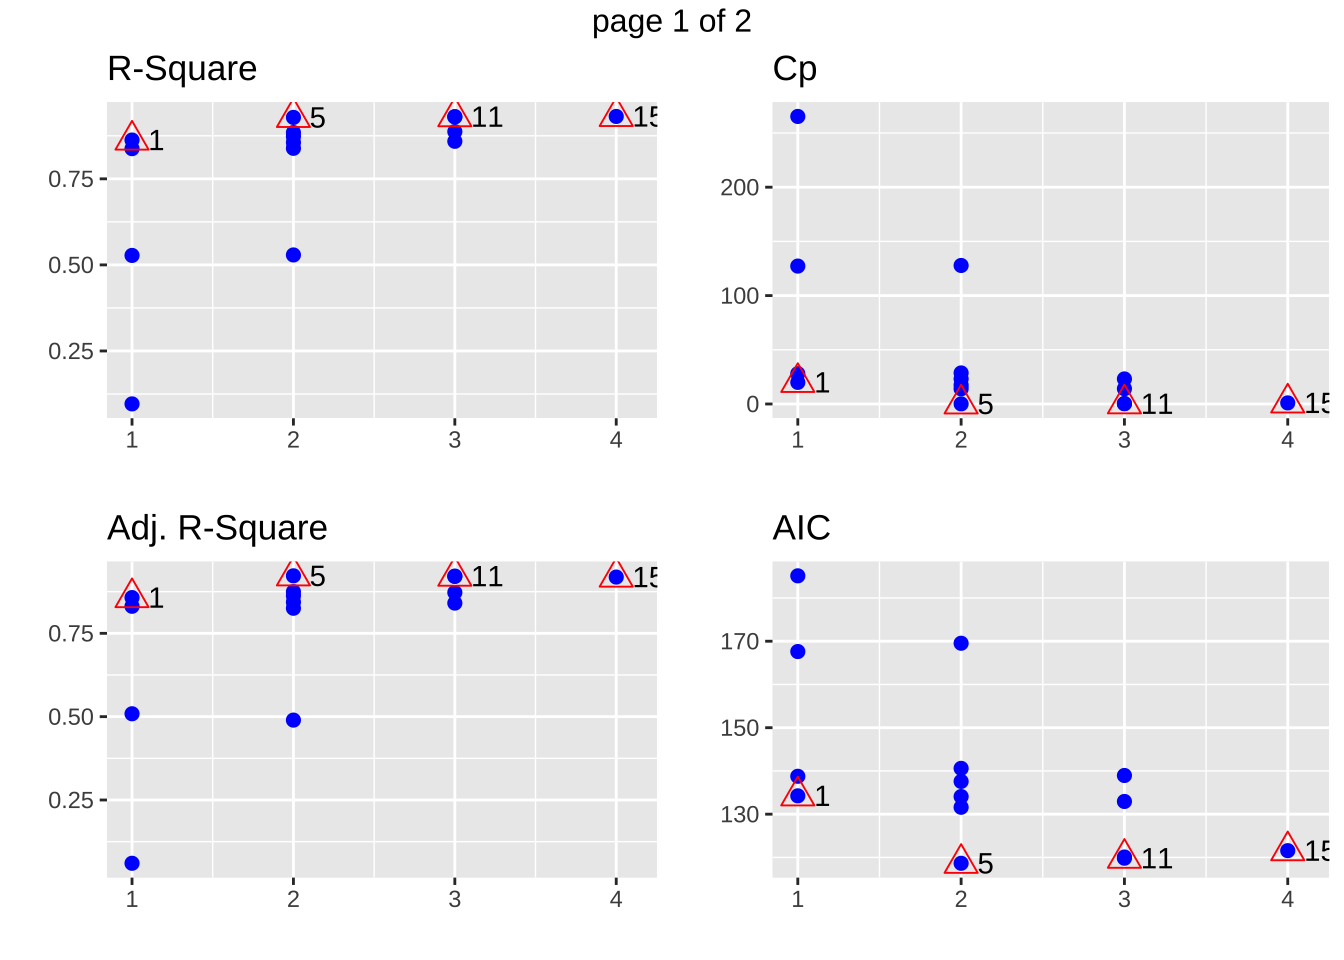
\includegraphics{lmpractice_files/figure-latex/unnamed-chunk-111-1.pdf} 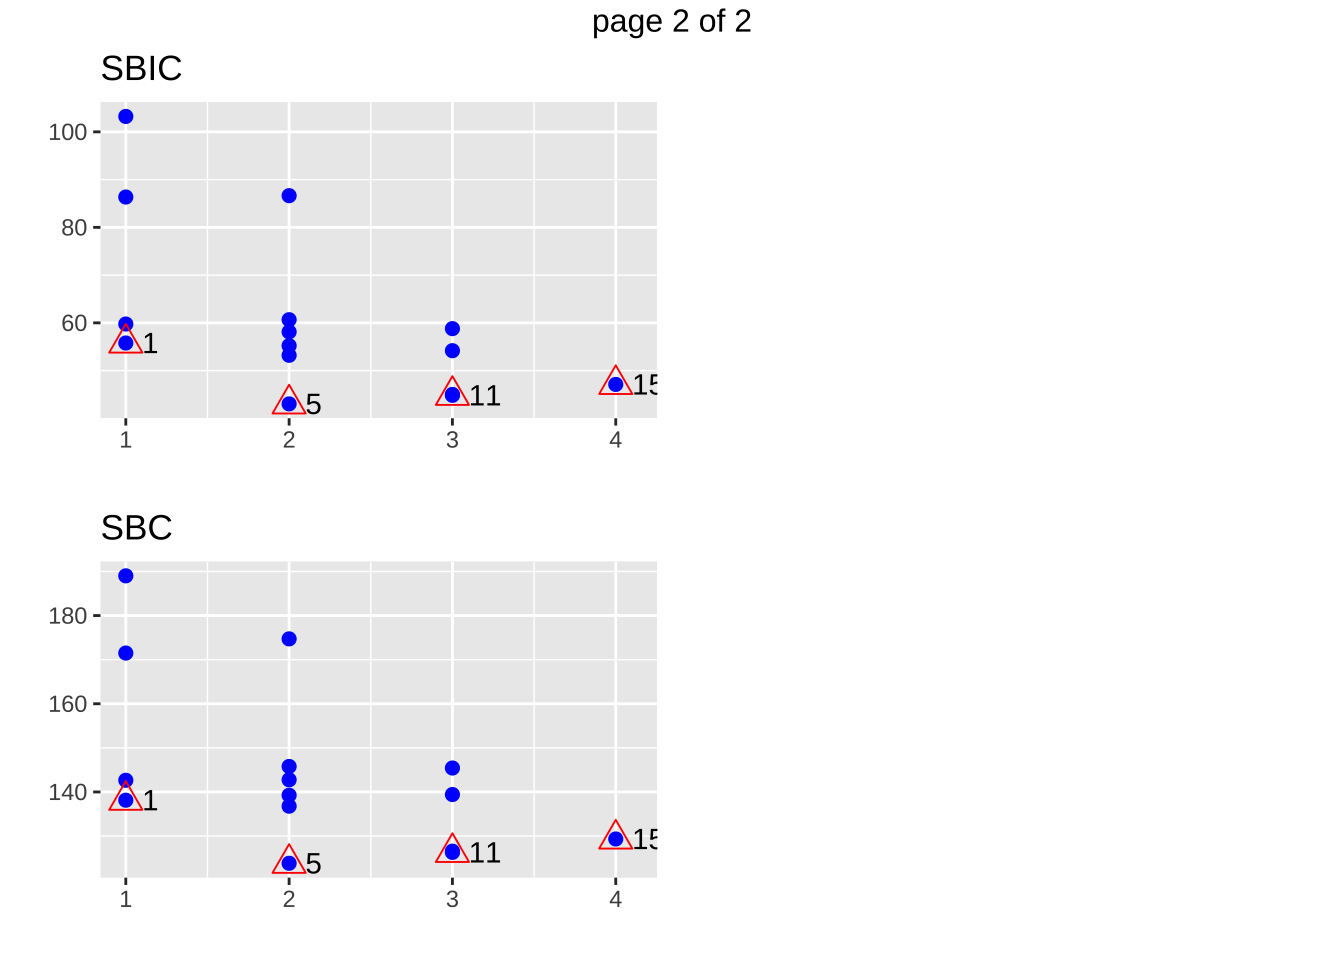
\includegraphics{lmpractice_files/figure-latex/unnamed-chunk-111-2.pdf}

맬로우의 \(C_p\) 를 나타내는 방법은 아래와 같이 선택된 독립변수의 개수에서 \(y=x\) 측에 가까운 값을 가진 모형이 좋은 모형이다.

\begin{Shaded}
\begin{Highlighting}[]
\FunctionTok{subsets}\NormalTok{(houseprice.rgs, }\AttributeTok{statistic=}\StringTok{"cp"}\NormalTok{, }\AttributeTok{legend =}\NormalTok{ F, }\AttributeTok{min.size =} \DecValTok{1}\NormalTok{, }\AttributeTok{main =} \StringTok{"Mallow Cp"}\NormalTok{,}\AttributeTok{ylim=}\FunctionTok{c}\NormalTok{(}\DecValTok{0}\NormalTok{,}\DecValTok{300}\NormalTok{))}
\end{Highlighting}
\end{Shaded}

\begin{verbatim}
##        Abbreviation
## tax               t
## ground            g
## floor             f
## year              y
\end{verbatim}

\begin{Shaded}
\begin{Highlighting}[]
\FunctionTok{abline}\NormalTok{(}\AttributeTok{a =} \DecValTok{1}\NormalTok{, }\AttributeTok{b =} \DecValTok{1}\NormalTok{, }\AttributeTok{lty =} \DecValTok{2}\NormalTok{)}
\end{Highlighting}
\end{Shaded}

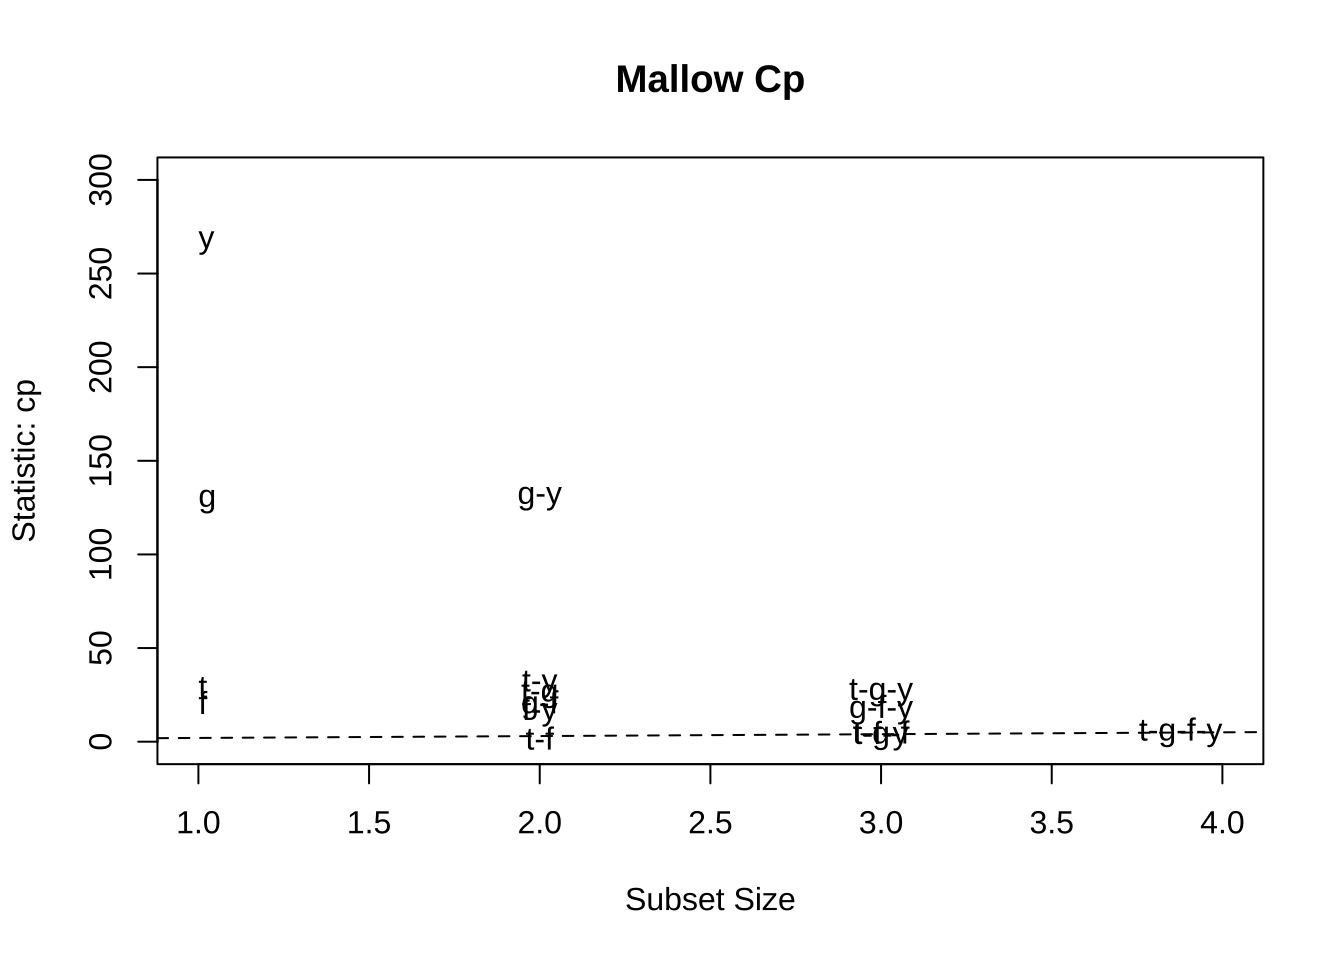
\includegraphics{lmpractice_files/figure-latex/unnamed-chunk-112-1.pdf}

PRESS 잔차는 함수 \texttt{press()} 로 구할 수 있다.

\[ PRESS_p = \sum_{i=1}^n ( y_i - \hat y_{i(i)})^2 \]

또한 교과서 264 페이지에 나온 교차확인(cross validation)에 의거한 \(R^2_{pred}\) 은 다음과 같이 계산되며 \texttt{press()} 함수에 의해 주어진다.

\[ R^2_{pred} = 1 - \frac{PRESS_p}{SST} \]

\begin{Shaded}
\begin{Highlighting}[]
\FunctionTok{press}\NormalTok{(houseprice.rgs)}
\end{Highlighting}
\end{Shaded}

\begin{verbatim}
##          tax ground floor year     PRESS pred.r.squared
## 1  ( 1 )                *       220.8853      0.8339932
## 1  ( 2 )   *                    316.0868      0.7624443
## 1  ( 3 )          *             838.8121      0.3695891
## 1  ( 4 )                     * 1430.6084      0.0000000
## 2  ( 1 )   *            *       144.3991      0.8914766
## 2  ( 2 )                *    *  207.6594      0.8439331
## 2  ( 3 )          *     *       233.7615      0.8243161
## 2  ( 4 )   *      *             358.2145      0.7307832
## 2  ( 5 )   *                 *  341.4294      0.7433981
## 2  ( 6 )          *          *  911.3553      0.3150691
## 3  ( 1 )   *            *    *  153.5941      0.8845661
## 3  ( 2 )   *      *     *       159.1752      0.8803716
## 3  ( 3 )          *     *    *  233.2240      0.8247200
## 3  ( 4 )   *      *          *  380.1744      0.7142792
## 4  ( 1 )   *      *     *    *  170.4810      0.8718747
\end{verbatim}

\hypertarget{uxc774uxc0c1uxce58uxb97c-uxc81cuxac70uxd55c-uxacbduxc6b0}{%
\section{이상치를 제거한 경우}\label{uxc774uxc0c1uxce58uxb97c-uxc81cuxac70uxd55c-uxacbduxc6b0}}

교과서에서 분석하였듯이 9,10,27 번째 자료가 이상점 또는 영향점일 가능성이 높으므로 이를 제거하고 모형의 선택 기준을 다시 계산해 보자.

\begin{Shaded}
\begin{Highlighting}[]
\NormalTok{housepriceEX }\OtherTok{\textless{}{-}}\NormalTok{ houseprice[}\SpecialCharTok{{-}}\FunctionTok{c}\NormalTok{(}\DecValTok{9}\NormalTok{,}\DecValTok{10}\NormalTok{,}\DecValTok{27}\NormalTok{),]}
\NormalTok{housepriceEX.rgs }\OtherTok{\textless{}{-}} \FunctionTok{regsubsets}\NormalTok{(price }\SpecialCharTok{\textasciitilde{}}\NormalTok{ . , }\AttributeTok{data=}\NormalTok{housepriceEX, }\AttributeTok{nbest=}\DecValTok{6}\NormalTok{)}
\FunctionTok{summaryf}\NormalTok{(housepriceEX.rgs)}
\end{Highlighting}
\end{Shaded}

\begin{verbatim}
##          tax ground floor year       rss       rsq     adjr2         cp        bic
## 1  ( 1 )   *                    48.17790 0.7675502 0.7569843  0.2458362 -28.661838
## 1  ( 2 )                *      102.73566 0.5043188 0.4817878 23.1726808 -10.487628
## 1  ( 3 )          *            125.87070 0.3926964 0.3650917 32.8947363  -5.613326
## 1  ( 4 )                     * 174.34503 0.1588164 0.1205808 53.2651405   2.205420
## 2  ( 1 )   *            *       46.18667 0.7771576 0.7559345  1.4090560 -26.496810
## 2  ( 2 )   *      *             47.39011 0.7713512 0.7495751  1.9147822 -25.879469
## 2  ( 3 )   *                 *  48.11577 0.7678500 0.7457405  2.2197243 -25.514758
## 2  ( 4 )                *    *  83.74651 0.5959380 0.5574559 17.1928590 -12.214327
## 2  ( 5 )          *     *       85.27968 0.5885408 0.5493542 17.8371405 -11.778929
## 2  ( 6 )          *          * 116.96847 0.4356480 0.3819002 31.1537464  -4.195690
## 3  ( 1 )   *      *     *       45.62514 0.7798669 0.7468469  3.1730851 -23.612331
## 3  ( 2 )   *            *    *  45.69348 0.7795371 0.7464677  3.2018056 -23.576407
## 3  ( 3 )   *      *          *  47.34784 0.7715551 0.7372884  3.8970174 -22.722834
## 3  ( 4 )          *     *    *  74.63053 0.6399210 0.5859092 15.3620431 -11.802150
## 4  ( 1 )   *      *     *    *  45.21326 0.7818541 0.7359287  5.0000000 -20.651921
\end{verbatim}

\begin{Shaded}
\begin{Highlighting}[]
\FunctionTok{press}\NormalTok{(housepriceEX.rgs)}
\end{Highlighting}
\end{Shaded}

\begin{verbatim}
##          tax ground floor year     PRESS pred.r.squared
## 1  ( 1 )   *                    56.10399     0.72930829
## 1  ( 2 )                *      117.36430     0.43373824
## 1  ( 3 )          *            157.83378     0.23848023
## 1  ( 4 )                     * 202.40162     0.02344834
## 2  ( 1 )   *            *       57.66354     0.72178375
## 2  ( 2 )   *      *             64.24819     0.69001399
## 2  ( 3 )   *                 *  63.42708     0.69397570
## 2  ( 4 )                *    * 108.09369     0.47846724
## 2  ( 5 )          *     *      114.27185     0.44865875
## 2  ( 6 )          *          * 160.37982     0.22619605
## 3  ( 1 )   *      *     *       68.98320     0.66716837
## 3  ( 2 )   *            *    *  65.44694     0.68423019
## 3  ( 3 )   *      *          *  72.26745     0.65132247
## 3  ( 4 )          *     *    * 109.76504     0.47040332
## 4  ( 1 )   *      *     *    *  79.24660     0.61764930
\end{verbatim}

\hypertarget{uxbcc0uxc218uxc120uxd0dd-uxbc29uxbc95}{%
\section{변수선택 방법}\label{uxbcc0uxc218uxc120uxd0dd-uxbc29uxbc95}}

회귀식에서 변수를을 선택할 때 가장 큰 모형을 적합시키면 각 변수에 대한 중요도를 각 회귀계수에 대한
가설 검정 \(H_o: \beta_i=0\)에 대한 t-통계량을 보고 판단할 수 있다.

\begin{Shaded}
\begin{Highlighting}[]
\FunctionTok{summary}\NormalTok{(fit1)}
\end{Highlighting}
\end{Shaded}

\begin{verbatim}
## 
## Call:
## lm(formula = price ~ ., data = houseprice)
## 
## Residuals:
##     Min      1Q  Median      3Q     Max 
## -3.4891 -1.3574  0.1337  1.0686  3.4938 
## 
## Coefficients:
##             Estimate Std. Error t value Pr(>|t|)    
## (Intercept)  1.21874    2.04661   0.595  0.55759    
## tax          0.05195    0.01383   3.756  0.00109 ** 
## ground       0.01159    0.02534   0.458  0.65169    
## floor        0.34941    0.07268   4.807 8.41e-05 ***
## year        -0.21894    0.33149  -0.660  0.51582    
## ---
## Signif. codes:  0 '***' 0.001 '**' 0.01 '*' 0.05 '.' 0.1 ' ' 1
## 
## Residual standard error: 2.039 on 22 degrees of freedom
## Multiple R-squared:  0.9313, Adjusted R-squared:  0.9188 
## F-statistic: 74.53 on 4 and 22 DF,  p-value: 1.817e-12
\end{verbatim}

위는 4개의 독립변수를 포함한 가장 큰 모형에 대하여 각 계수의 유의성 검정에 대한 결과이다.
변수 \texttt{floor}가 가장 유의한 변수이고 다음으로 \texttt{tax}가 유의함을 알 수 있다. 또한
2개의 변수 \texttt{year}와 \texttt{ground}는 유의하지 않음을 알 수 있다.

이렇게 독립변수들은 반응변수를 설명하는 정도가 다르므로 모든 가능한 회귀식을 적합하여 모형을 선택하는 것보다
변수의 중요도를 고려하여 변수들을 유의한 정도에 따라 차례로 모형에 포함시키거나 제거하는 절차가 더 효율적이다. 이렇게 가장 단순한 모형(평균모형)에서 시작하여 설명력이 높은 변수들을 순차적으로 포함시키거나(forward selection; 전진선택) 가장 큰 모형(full model)에서 시작하여 설명력이 낮은 변수들을
차례로 제거하는 방법(backward elimination; 후방제거)을 단계별 회귀(stepwise regression)이라고 한다.

단계별 회귀는 다음과 같은 세 가지 방법이 있다.

\begin{itemize}
\tightlist
\item
  전진선택 (forward selection)
\item
  후방제거 (backward elimination)
\item
  단계별 선택 (stepwise selection)
\end{itemize}

단계별 선택은 전진선택과 후방제거를 결합한 형태로서 새로운 변수가 추가되는 경우마다(전진선택) 제거할 변수를 있는지 판단하여 유의하지 않다면 제거하는(후방제거) 방법이다.

\hypertarget{uxb2e8uxacc4uxbcc4-uxc120uxd0dduxc758-uxc801uxc6a9}{%
\subsection{단계별 선택의 적용}\label{uxb2e8uxacc4uxbcc4-uxc120uxd0dduxc758-uxc801uxc6a9}}

단계별 선택에서 전진선택과 후방제거는 \texttt{add1()}와 \texttt{drop1()}함수를 사용한다.

\hypertarget{uxd3c9uxade0uxbaa8uxd615}{%
\subsubsection{평균모형}\label{uxd3c9uxade0uxbaa8uxd615}}

\begin{Shaded}
\begin{Highlighting}[]
\NormalTok{model0 }\OtherTok{\textless{}{-}} \FunctionTok{lm}\NormalTok{(price}\SpecialCharTok{\textasciitilde{}}\DecValTok{1}\NormalTok{, houseprice)}
\FunctionTok{summary}\NormalTok{(model0)}
\end{Highlighting}
\end{Shaded}

\begin{verbatim}
## 
## Call:
## lm(formula = price ~ 1, data = houseprice)
## 
## Residuals:
##    Min     1Q Median     3Q    Max 
## -6.300 -4.275 -0.800  1.125 23.200 
## 
## Coefficients:
##             Estimate Std. Error t value Pr(>|t|)    
## (Intercept)   19.250      1.377   13.98 1.32e-13 ***
## ---
## Signif. codes:  0 '***' 0.001 '**' 0.01 '*' 0.05 '.' 0.1 ' ' 1
## 
## Residual standard error: 7.154 on 26 degrees of freedom
\end{verbatim}

\hypertarget{uxccabuxbc88uxc9f8-uxbcc0uxc218uxc758-uxcd94uxac00}{%
\subsubsection{첫번째 변수의 추가}\label{uxccabuxbc88uxc9f8-uxbcc0uxc218uxc758-uxcd94uxac00}}

이제 가장 설명력있는 변수를 추가하는데 다음과 같은 2개의 모형을 비교하는 부분 F 검정을 이용하여 가장 유의한 변수를 추가한다.

\[ H_0: y=\beta_0 + \epsilon \quad \text{vs} \quad y=\beta_0 + \beta_1 x_i + \epsilon \]

\begin{Shaded}
\begin{Highlighting}[]
\FunctionTok{add1}\NormalTok{(model0, }\AttributeTok{scope=}\SpecialCharTok{\textasciitilde{}}\NormalTok{tax}\SpecialCharTok{+}\NormalTok{ ground}\SpecialCharTok{+}\NormalTok{ floor}\SpecialCharTok{+}\NormalTok{ year, }\AttributeTok{test=}\StringTok{"F"}\NormalTok{)}
\end{Highlighting}
\end{Shaded}

\begin{verbatim}
## Single term additions
## 
## Model:
## price ~ 1
##        Df Sum of Sq     RSS     AIC  F value    Pr(>F)    
## <none>              1330.58 107.233                       
## tax     1   1114.60  215.98  60.142 129.0183 2.310e-11 ***
## ground  1    701.96  628.62  88.987  27.9170 1.792e-05 ***
## floor   1   1147.92  182.66  55.619 157.1084 2.807e-12 ***
## year    1    128.11 1202.47 106.500   2.6634    0.1152    
## ---
## Signif. codes:  0 '***' 0.001 '**' 0.01 '*' 0.05 '.' 0.1 ' ' 1
\end{verbatim}

위의 결과에서 가장 유의한 변수가 \texttt{floor}이므로 회귀식에 추가한다. 변수를 추가하는 경우는 고려하는 변수를 포함한 모형과 포함하지 않는 모형이 가장 유의한 차이를 보이는 변수를 선택한다.

\begin{Shaded}
\begin{Highlighting}[]
\NormalTok{model1 }\OtherTok{\textless{}{-}} \FunctionTok{update}\NormalTok{(model0, . }\SpecialCharTok{\textasciitilde{}}\NormalTok{ . }\SpecialCharTok{+}\NormalTok{ floor)}
\FunctionTok{summary}\NormalTok{(model1)}
\end{Highlighting}
\end{Shaded}

\begin{verbatim}
## 
## Call:
## lm(formula = price ~ floor, data = houseprice)
## 
## Residuals:
##     Min      1Q  Median      3Q     Max 
## -4.6682 -2.1916 -0.1459  2.0517  4.9644 
## 
## Coefficients:
##             Estimate Std. Error t value Pr(>|t|)    
## (Intercept)  1.25296    1.52716    0.82     0.42    
## floor        0.59511    0.04748   12.53 2.81e-12 ***
## ---
## Signif. codes:  0 '***' 0.001 '**' 0.01 '*' 0.05 '.' 0.1 ' ' 1
## 
## Residual standard error: 2.703 on 25 degrees of freedom
## Multiple R-squared:  0.8627, Adjusted R-squared:  0.8572 
## F-statistic: 157.1 on 1 and 25 DF,  p-value: 2.807e-12
\end{verbatim}

위에서 \texttt{update()} 함수는 앞에서 적합한 모형 \texttt{model0}에 변수 \texttt{floor}를 추가한다.

\hypertarget{uxb450-uxbc88uxc9f8-uxbcc0uxc218uxc758-uxcd94uxac00}{%
\subsubsection{두 번째 변수의 추가}\label{uxb450-uxbc88uxc9f8-uxbcc0uxc218uxc758-uxcd94uxac00}}

\begin{Shaded}
\begin{Highlighting}[]
\FunctionTok{add1}\NormalTok{(model1, }\AttributeTok{scope=}\SpecialCharTok{\textasciitilde{}}\NormalTok{tax}\SpecialCharTok{+}\NormalTok{ ground}\SpecialCharTok{+}\NormalTok{ floor}\SpecialCharTok{+}\NormalTok{ year, }\AttributeTok{test=}\StringTok{"F"}\NormalTok{)}
\end{Highlighting}
\end{Shaded}

\begin{verbatim}
## Single term additions
## 
## Model:
## price ~ floor
##        Df Sum of Sq     RSS    AIC F value    Pr(>F)    
## <none>              182.663 55.619                      
## tax     1    87.468  95.195 40.023 22.0517 8.997e-05 ***
## ground  1    14.075 168.588 55.454  2.0037   0.16976    
## year    1    28.854 153.809 52.977  4.5023   0.04437 *  
## ---
## Signif. codes:  0 '***' 0.001 '**' 0.01 '*' 0.05 '.' 0.1 ' ' 1
\end{verbatim}

\begin{Shaded}
\begin{Highlighting}[]
\NormalTok{model2 }\OtherTok{\textless{}{-}} \FunctionTok{update}\NormalTok{(model1, . }\SpecialCharTok{\textasciitilde{}}\NormalTok{ . }\SpecialCharTok{+}\NormalTok{ tax)}
\FunctionTok{summary}\NormalTok{(model2)}
\end{Highlighting}
\end{Shaded}

\begin{verbatim}
## 
## Call:
## lm(formula = price ~ floor + tax, data = houseprice)
## 
## Residuals:
##    Min     1Q Median     3Q    Max 
## -3.009 -1.658  0.048  1.220  3.548 
## 
## Coefficients:
##             Estimate Std. Error t value Pr(>|t|)    
## (Intercept)  0.39497    1.13994   0.346    0.732    
## floor        0.34835    0.06313   5.518 1.13e-05 ***
## tax          0.05742    0.01223   4.696 9.00e-05 ***
## ---
## Signif. codes:  0 '***' 0.001 '**' 0.01 '*' 0.05 '.' 0.1 ' ' 1
## 
## Residual standard error: 1.992 on 24 degrees of freedom
## Multiple R-squared:  0.9285, Adjusted R-squared:  0.9225 
## F-statistic: 155.7 on 2 and 24 DF,  p-value: 1.798e-14
\end{verbatim}

위의 결과로부터 변수 \texttt{tax}가 가장 유의한 변수임을 알 수 있고 이를 모형에 추가한다.

\hypertarget{uxbcc0uxc218uxc758-uxc81cuxac70}{%
\subsubsection{변수의 제거}\label{uxbcc0uxc218uxc758-uxc81cuxac70}}

이제 독립변수가 두 개가(\texttt{floor}와 \texttt{tax}) 모형에 포함되었고 가장 최근에 포함된 변수 \texttt{tax}를 제외한
나머지 변수를 제거할 수 있는지 감정한다. 후방제거하는 경우는 제거할 변수가 포함된 모형과 포함하지 않는 모형의
설명력에 유의한 차이가 없어야 한다. 즉 F-검정이 유의하니 않으면 제거한다.

\begin{Shaded}
\begin{Highlighting}[]
\FunctionTok{drop1}\NormalTok{(model2, }\AttributeTok{test=}\StringTok{"F"}\NormalTok{)}
\end{Highlighting}
\end{Shaded}

\begin{verbatim}
## Single term deletions
## 
## Model:
## price ~ floor + tax
##        Df Sum of Sq     RSS    AIC F value    Pr(>F)    
## <none>               95.195 40.023                      
## floor   1   120.782 215.978 60.142  30.451 1.126e-05 ***
## tax     1    87.468 182.663 55.619  22.052 8.997e-05 ***
## ---
## Signif. codes:  0 '***' 0.001 '**' 0.01 '*' 0.05 '.' 0.1 ' ' 1
\end{verbatim}

위의 함수 \texttt{drop1()}의 결과에서 모든 변수에 대한 F-통계량이 유의하므로 변수를 제거하지 않는다.

\hypertarget{uxc138-uxbc88uxc9f8-uxbcc0uxc218uxc758-uxcd94uxac00}{%
\subsubsection{세 번째 변수의 추가}\label{uxc138-uxbc88uxc9f8-uxbcc0uxc218uxc758-uxcd94uxac00}}

독립변수가 두 개가(\texttt{floor}와 \texttt{tax}) 모형에 새로운 변수를 추가하는 검정을 실시해 보자

\begin{Shaded}
\begin{Highlighting}[]
\FunctionTok{add1}\NormalTok{(model2, }\AttributeTok{scope=}\SpecialCharTok{\textasciitilde{}}\NormalTok{tax}\SpecialCharTok{+}\NormalTok{ ground}\SpecialCharTok{+}\NormalTok{ floor}\SpecialCharTok{+}\NormalTok{ year, }\AttributeTok{test=}\StringTok{"F"}\NormalTok{)}
\end{Highlighting}
\end{Shaded}

\begin{verbatim}
## Single term additions
## 
## Model:
## price ~ floor + tax
##        Df Sum of Sq    RSS    AIC F value Pr(>F)
## <none>              95.195 40.023               
## ground  1    1.9335 93.262 41.469  0.4768 0.4968
## year    1    2.8761 92.319 41.194  0.7165 0.4060
\end{verbatim}

위의 결과에서 유의한 변수가 없으므로 더 이상 변수를 추가하지 않는다.

\hypertarget{uxcd5cuxc885-uxbaa8uxd615}{%
\subsubsection{최종 모형}\label{uxcd5cuxc885-uxbaa8uxd615}}

더 이상 추가할 변수와 제거할 변수가 없으면 단계별 선택을 중단한다. 따라서 단계별 선택법에 의한
최종 모형은 \texttt{floor}와 \texttt{tax}, 두 개의 독립변수를 포함하는 모형이다.

이러한 단계별 회귀의 결과는 모든 가능한 회귀에 의한 방법과 모형이 일치한다. 독립변수의 수가 많는 경우 이러한 단계별 회귀 방법은 유용하게 사용된다.

\hypertarget{uxd568uxc218-step}{%
\subsection{\texorpdfstring{함수 \texttt{step()}}{함수 step()}}\label{uxd568uxc218-step}}

위에서 논의한 세종류의 변수선택법은 함수 \texttt{step()}을 이용하여 한 번에 결과를 얻을 수 있다.

\begin{rmdcaution}
주의할 점은 함수 \texttt{step()}은 변수의 선택 기준이 F-검정이 아니 AIC 를 이용한다는 점이다.
\end{rmdcaution}

\hypertarget{uxc804uxc9c4uxc120uxd0dduxbc95}{%
\subsubsection{전진선택법}\label{uxc804uxc9c4uxc120uxd0dduxbc95}}

\begin{Shaded}
\begin{Highlighting}[]
\NormalTok{model0 }\OtherTok{\textless{}{-}} \FunctionTok{lm}\NormalTok{(price}\SpecialCharTok{\textasciitilde{}}\DecValTok{1}\NormalTok{, houseprice)}
\FunctionTok{step}\NormalTok{(model0,  }\AttributeTok{scope=}\SpecialCharTok{\textasciitilde{}}\NormalTok{tax}\SpecialCharTok{+}\NormalTok{ ground}\SpecialCharTok{+}\NormalTok{ floor}\SpecialCharTok{+}\NormalTok{ year, }\AttributeTok{direction=}\StringTok{"forward"}\NormalTok{)}
\end{Highlighting}
\end{Shaded}

\begin{verbatim}
## Start:  AIC=107.23
## price ~ 1
## 
##          Df Sum of Sq     RSS     AIC
## + floor   1   1147.92  182.66  55.619
## + tax     1   1114.60  215.98  60.142
## + ground  1    701.96  628.62  88.987
## + year    1    128.11 1202.47 106.500
## <none>                1330.58 107.233
## 
## Step:  AIC=55.62
## price ~ floor
## 
##          Df Sum of Sq     RSS    AIC
## + tax     1    87.468  95.195 40.023
## + year    1    28.854 153.809 52.977
## + ground  1    14.075 168.588 55.454
## <none>                182.663 55.619
## 
## Step:  AIC=40.02
## price ~ floor + tax
## 
##          Df Sum of Sq    RSS    AIC
## <none>                95.195 40.023
## + year    1    2.8761 92.319 41.194
## + ground  1    1.9335 93.262 41.469
\end{verbatim}

\begin{verbatim}
## 
## Call:
## lm(formula = price ~ floor + tax, data = houseprice)
## 
## Coefficients:
## (Intercept)        floor          tax  
##     0.39497      0.34835      0.05742
\end{verbatim}

\hypertarget{uxd6c4uxbc29uxc81cuxac70}{%
\subsubsection{후방제거}\label{uxd6c4uxbc29uxc81cuxac70}}

\begin{Shaded}
\begin{Highlighting}[]
\NormalTok{fit }\OtherTok{\textless{}{-}} \FunctionTok{lm}\NormalTok{(price}\SpecialCharTok{\textasciitilde{}}\NormalTok{tax}\SpecialCharTok{+}\NormalTok{ ground}\SpecialCharTok{+}\NormalTok{ floor}\SpecialCharTok{+}\NormalTok{ year, houseprice)}
\FunctionTok{step}\NormalTok{(fit, }\AttributeTok{direction=}\StringTok{"backward"}\NormalTok{)}
\end{Highlighting}
\end{Shaded}

\begin{verbatim}
## Start:  AIC=42.94
## price ~ tax + ground + floor + year
## 
##          Df Sum of Sq     RSS    AIC
## - ground  1     0.871  92.319 41.194
## - year    1     1.813  93.262 41.469
## <none>                 91.449 42.938
## - tax     1    58.652 150.100 54.318
## - floor   1    96.064 187.513 60.326
## 
## Step:  AIC=41.19
## price ~ tax + floor + year
## 
##         Df Sum of Sq     RSS    AIC
## - year   1     2.876  95.195 40.023
## <none>                92.319 41.194
## - tax    1    61.490 153.809 52.977
## - floor  1   122.322 214.642 61.975
## 
## Step:  AIC=40.02
## price ~ tax + floor
## 
##         Df Sum of Sq     RSS    AIC
## <none>                95.195 40.023
## - tax    1    87.468 182.663 55.619
## - floor  1   120.782 215.978 60.142
\end{verbatim}

\begin{verbatim}
## 
## Call:
## lm(formula = price ~ tax + floor, data = houseprice)
## 
## Coefficients:
## (Intercept)          tax        floor  
##     0.39497      0.05742      0.34835
\end{verbatim}

\hypertarget{uxb2e8uxacc4uxbcc4-uxc120uxd0dd}{%
\subsubsection{단계별 선택}\label{uxb2e8uxacc4uxbcc4-uxc120uxd0dd}}

\begin{Shaded}
\begin{Highlighting}[]
\NormalTok{model0 }\OtherTok{\textless{}{-}} \FunctionTok{lm}\NormalTok{(price}\SpecialCharTok{\textasciitilde{}}\DecValTok{1}\NormalTok{, houseprice)}
\FunctionTok{step}\NormalTok{(model0,  }\AttributeTok{scope=}\SpecialCharTok{\textasciitilde{}}\NormalTok{tax}\SpecialCharTok{+}\NormalTok{ ground}\SpecialCharTok{+}\NormalTok{ floor}\SpecialCharTok{+}\NormalTok{ year, }\AttributeTok{direction=}\StringTok{"both"}\NormalTok{)}
\end{Highlighting}
\end{Shaded}

\begin{verbatim}
## Start:  AIC=107.23
## price ~ 1
## 
##          Df Sum of Sq     RSS     AIC
## + floor   1   1147.92  182.66  55.619
## + tax     1   1114.60  215.98  60.142
## + ground  1    701.96  628.62  88.987
## + year    1    128.11 1202.47 106.500
## <none>                1330.58 107.233
## 
## Step:  AIC=55.62
## price ~ floor
## 
##          Df Sum of Sq     RSS     AIC
## + tax     1     87.47   95.20  40.023
## + year    1     28.85  153.81  52.977
## + ground  1     14.08  168.59  55.454
## <none>                 182.66  55.619
## - floor   1   1147.92 1330.58 107.233
## 
## Step:  AIC=40.02
## price ~ floor + tax
## 
##          Df Sum of Sq     RSS    AIC
## <none>                 95.195 40.023
## + year    1     2.876  92.319 41.194
## + ground  1     1.934  93.262 41.469
## - tax     1    87.468 182.663 55.619
## - floor   1   120.782 215.978 60.142
\end{verbatim}

\begin{verbatim}
## 
## Call:
## lm(formula = price ~ floor + tax, data = houseprice)
## 
## Coefficients:
## (Intercept)        floor          tax  
##     0.39497      0.34835      0.05742
\end{verbatim}

\hypertarget{uxd328uxd0a4uxc9c0-olsrr}{%
\subsection{\texorpdfstring{패키지 \texttt{olsrr}}{패키지 olsrr}}\label{uxd328uxd0a4uxc9c0-olsrr}}

패키지 \texttt{olsrr} 의 함수 \texttt{ols\_step\_both\_p()} 이용하여 F-검정을 이용한 단계별 선택을 할 수 있다.

\begin{rmdcaution}
함수 \texttt{ols\_step\_both\_p()} 이용하여 F-검정에서는 유의수준을 지정해주지 않으면
유의 수준을 0.3 으로 사용한다.

참고로 SAS 의 모형 선택에서 자동적으로 사용되는 유의수준은 전진선택에서는 0.5, 후방제거에서는 0.1 이다.\\
\end{rmdcaution}

\begin{verbatim}
ols_step_forward_p(model, penter = 0.3,
  progress = FALSE, details = FALSE, ...)
ols_step_backward_p(model, prem = 0.3,
  progress = FALSE, details = FALSE, ...)

Forward Selection (FORWARD)

The p-values for these F statistics are compared to the SLENTRY= value that is specified in the MODEL statement (or to 0.50 if the SLENTRY= option is omitted). 

Backward Elimination (BACKWARD)

F statistics significant at the SLSTAY= level specified in the MODEL statement (or at the 0.10 level if the SLSTAY= option is omitted). 
\end{verbatim}

\begin{Shaded}
\begin{Highlighting}[]
\NormalTok{res }\OtherTok{\textless{}{-}} \FunctionTok{ols\_step\_both\_p}\NormalTok{(fit1, }\AttributeTok{details =} \ConstantTok{TRUE}\NormalTok{)}
\end{Highlighting}
\end{Shaded}

\begin{verbatim}
## Stepwise Selection Method   
## ---------------------------
## 
## Candidate Terms: 
## 
## 1. tax 
## 2. ground 
## 3. floor 
## 4. year 
## 
## We are selecting variables based on p value...
## 
## 
## Stepwise Selection: Step 1 
## 
## - floor added 
## 
##                         Model Summary                          
## --------------------------------------------------------------
## R                       0.929       RMSE                2.703 
## R-Squared               0.863       Coef. Var          14.042 
## Adj. R-Squared          0.857       MSE                 7.307 
## Pred R-Squared          0.834       MAE                 2.182 
## --------------------------------------------------------------
##  RMSE: Root Mean Square Error 
##  MSE: Mean Square Error 
##  MAE: Mean Absolute Error 
## 
##                                 ANOVA                                 
## ---------------------------------------------------------------------
##                 Sum of                                               
##                Squares        DF    Mean Square       F         Sig. 
## ---------------------------------------------------------------------
## Regression    1147.917         1       1147.917    157.108    0.0000 
## Residual       182.663        25          7.307                      
## Total         1330.580        26                                     
## ---------------------------------------------------------------------
## 
##                                  Parameter Estimates                                   
## --------------------------------------------------------------------------------------
##       model     Beta    Std. Error    Std. Beta      t        Sig      lower    upper 
## --------------------------------------------------------------------------------------
## (Intercept)    1.253         1.527                  0.820    0.420    -1.892    4.398 
##       floor    0.595         0.047        0.929    12.534    0.000     0.497    0.693 
## --------------------------------------------------------------------------------------
## 
## 
## 
## Stepwise Selection: Step 2 
## 
## - tax added 
## 
##                         Model Summary                          
## --------------------------------------------------------------
## R                       0.964       RMSE                1.992 
## R-Squared               0.928       Coef. Var          10.346 
## Adj. R-Squared          0.922       MSE                 3.966 
## Pred R-Squared          0.891       MAE                 1.572 
## --------------------------------------------------------------
##  RMSE: Root Mean Square Error 
##  MSE: Mean Square Error 
##  MAE: Mean Absolute Error 
## 
##                                 ANOVA                                 
## ---------------------------------------------------------------------
##                 Sum of                                               
##                Squares        DF    Mean Square       F         Sig. 
## ---------------------------------------------------------------------
## Regression    1235.385         2        617.692    155.728    0.0000 
## Residual        95.195        24          3.966                      
## Total         1330.580        26                                     
## ---------------------------------------------------------------------
## 
##                                  Parameter Estimates                                  
## -------------------------------------------------------------------------------------
##       model     Beta    Std. Error    Std. Beta      t       Sig      lower    upper 
## -------------------------------------------------------------------------------------
## (Intercept)    0.395         1.140                 0.346    0.732    -1.958    2.748 
##       floor    0.348         0.063        0.544    5.518    0.000     0.218    0.479 
##         tax    0.057         0.012        0.463    4.696    0.000     0.032    0.083 
## -------------------------------------------------------------------------------------
## 
## 
## 
##                         Model Summary                          
## --------------------------------------------------------------
## R                       0.964       RMSE                1.992 
## R-Squared               0.928       Coef. Var          10.346 
## Adj. R-Squared          0.922       MSE                 3.966 
## Pred R-Squared          0.891       MAE                 1.572 
## --------------------------------------------------------------
##  RMSE: Root Mean Square Error 
##  MSE: Mean Square Error 
##  MAE: Mean Absolute Error 
## 
##                                 ANOVA                                 
## ---------------------------------------------------------------------
##                 Sum of                                               
##                Squares        DF    Mean Square       F         Sig. 
## ---------------------------------------------------------------------
## Regression    1235.385         2        617.692    155.728    0.0000 
## Residual        95.195        24          3.966                      
## Total         1330.580        26                                     
## ---------------------------------------------------------------------
## 
##                                  Parameter Estimates                                  
## -------------------------------------------------------------------------------------
##       model     Beta    Std. Error    Std. Beta      t       Sig      lower    upper 
## -------------------------------------------------------------------------------------
## (Intercept)    0.395         1.140                 0.346    0.732    -1.958    2.748 
##       floor    0.348         0.063        0.544    5.518    0.000     0.218    0.479 
##         tax    0.057         0.012        0.463    4.696    0.000     0.032    0.083 
## -------------------------------------------------------------------------------------
## 
## 
## 
## No more variables to be added/removed.
## 
## 
## Final Model Output 
## ------------------
## 
##                         Model Summary                          
## --------------------------------------------------------------
## R                       0.964       RMSE                1.992 
## R-Squared               0.928       Coef. Var          10.346 
## Adj. R-Squared          0.922       MSE                 3.966 
## Pred R-Squared          0.891       MAE                 1.572 
## --------------------------------------------------------------
##  RMSE: Root Mean Square Error 
##  MSE: Mean Square Error 
##  MAE: Mean Absolute Error 
## 
##                                 ANOVA                                 
## ---------------------------------------------------------------------
##                 Sum of                                               
##                Squares        DF    Mean Square       F         Sig. 
## ---------------------------------------------------------------------
## Regression    1235.385         2        617.692    155.728    0.0000 
## Residual        95.195        24          3.966                      
## Total         1330.580        26                                     
## ---------------------------------------------------------------------
## 
##                                  Parameter Estimates                                  
## -------------------------------------------------------------------------------------
##       model     Beta    Std. Error    Std. Beta      t       Sig      lower    upper 
## -------------------------------------------------------------------------------------
## (Intercept)    0.395         1.140                 0.346    0.732    -1.958    2.748 
##       floor    0.348         0.063        0.544    5.518    0.000     0.218    0.479 
##         tax    0.057         0.012        0.463    4.696    0.000     0.032    0.083 
## -------------------------------------------------------------------------------------
\end{verbatim}

\begin{Shaded}
\begin{Highlighting}[]
\NormalTok{res}
\end{Highlighting}
\end{Shaded}

\begin{verbatim}
## 
##                              Stepwise Selection Summary                               
## -------------------------------------------------------------------------------------
##                      Added/                   Adj.                                       
## Step    Variable    Removed     R-Square    R-Square     C(p)        AIC        RMSE     
## -------------------------------------------------------------------------------------
##    1     floor      addition       0.863       0.857    20.9440    134.2415    2.7031    
##    2      tax       addition       0.928       0.922     1.9010    118.6453    1.9916    
## -------------------------------------------------------------------------------------
\end{verbatim}

\begin{Shaded}
\begin{Highlighting}[]
\FunctionTok{plot}\NormalTok{(res)}
\end{Highlighting}
\end{Shaded}

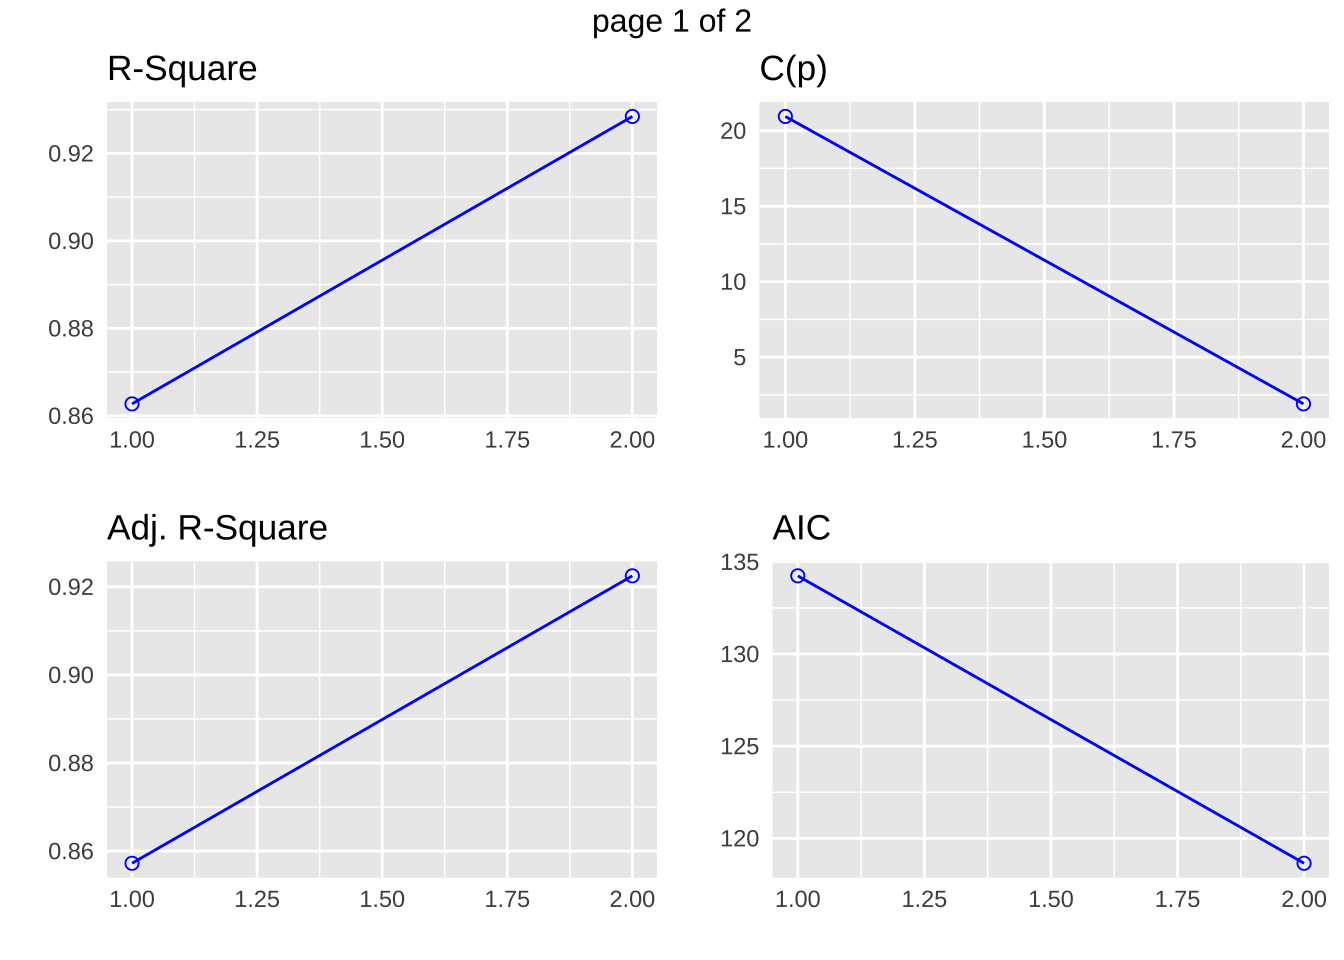
\includegraphics{lmpractice_files/figure-latex/unnamed-chunk-128-1.pdf} 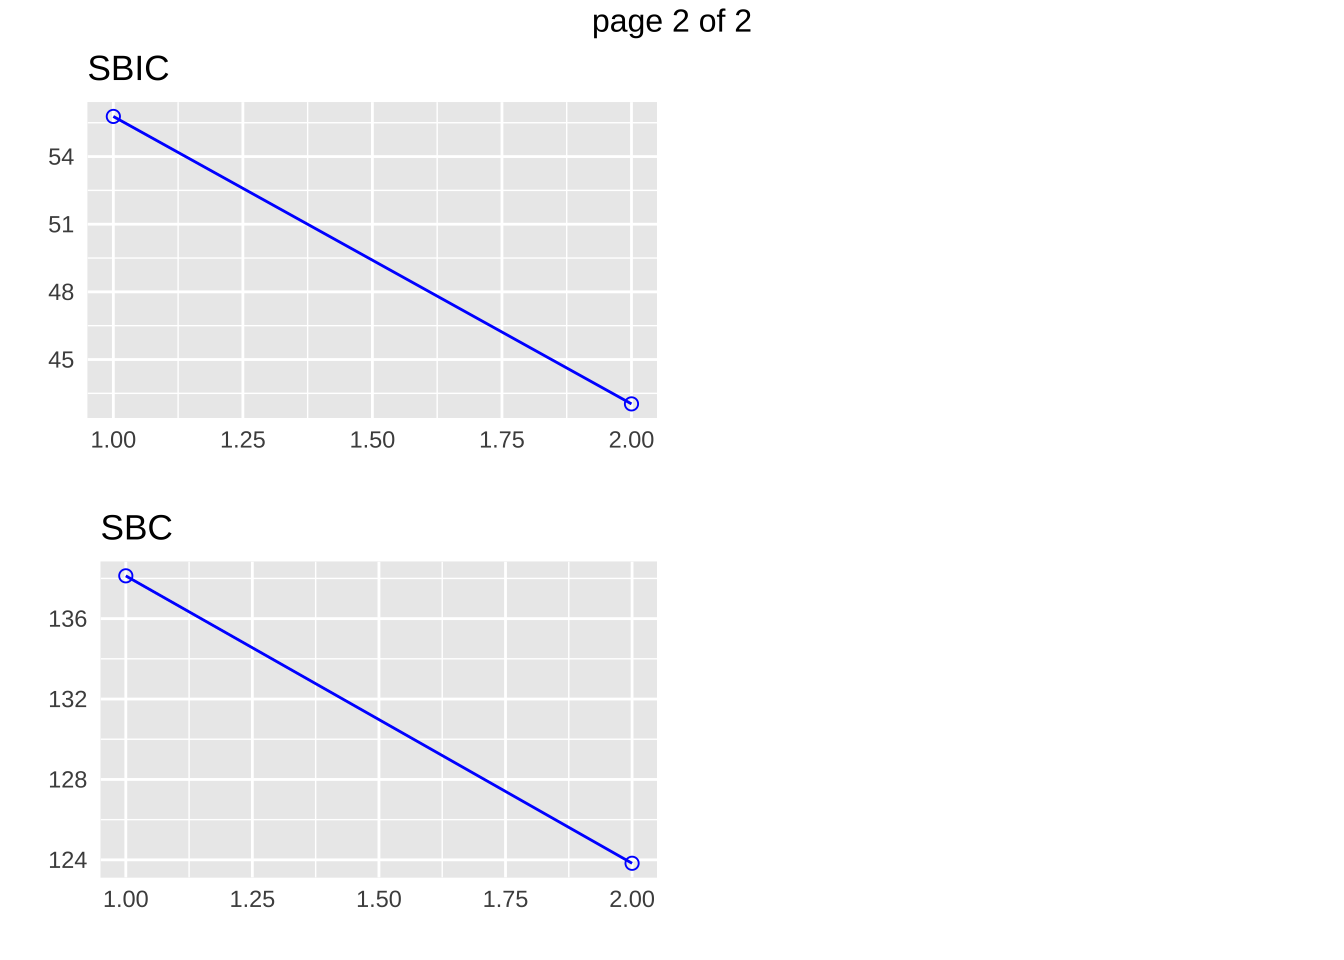
\includegraphics{lmpractice_files/figure-latex/unnamed-chunk-128-2.pdf}

함수 \texttt{ols\_step\_both\_aic()} 는 함수 \texttt{step()} 과 동일하게 AIC 를 이용하여 변수선택을 한다.

\begin{Shaded}
\begin{Highlighting}[]
\FunctionTok{ols\_step\_forward\_aic}\NormalTok{(fit1)}
\end{Highlighting}
\end{Shaded}

\begin{verbatim}
## 
##                          Selection Summary                          
## -------------------------------------------------------------------
## Variable       AIC       Sum Sq       RSS       R-Sq      Adj. R-Sq 
## -------------------------------------------------------------------
## floor        134.241    1147.917    182.663    0.86272      0.85723 
## tax          118.645    1235.385     95.195    0.92846      0.92249 
## -------------------------------------------------------------------
\end{verbatim}

\hypertarget{uxc5f0uxc2b5uxbb38uxc81c-6.10}{%
\section{연습문제 6.10}\label{uxc5f0uxc2b5uxbb38uxc81c-6.10}}

자료 \texttt{cars93}은 1993년 미국에서 판매된 93가지 종류의 저동차에 대한 자료이다. 변수 \texttt{MPG.highway}를 반응변수로 하고 \texttt{EngineSize}, \texttt{Weight}, \texttt{Price}, \texttt{Width}, \texttt{Length}, \texttt{Horsepower}, \texttt{Wheelbae} 7개의 변수를
고려하여 가장 적합한 모형을 선택해보자.

\begin{Shaded}
\begin{Highlighting}[]
\NormalTok{dat93 }\OtherTok{\textless{}{-}}\NormalTok{ Cars93[}\FunctionTok{c}\NormalTok{(}\StringTok{"MPG.highway"}\NormalTok{,}\StringTok{"EngineSize"}\NormalTok{, }\StringTok{"Weight"}\NormalTok{, }\StringTok{"Price"}\NormalTok{, }\StringTok{"Width"}\NormalTok{, }\StringTok{"Length"}\NormalTok{, }\StringTok{"Horsepower"}\NormalTok{, }\StringTok{"Wheelbase"}\NormalTok{)]}
\FunctionTok{head}\NormalTok{(dat93)}
\end{Highlighting}
\end{Shaded}

\begin{verbatim}
##   MPG.highway EngineSize Weight Price Width Length Horsepower Wheelbase
## 1          31        1.8   2705  15.9    68    177        140       102
## 2          25        3.2   3560  33.9    71    195        200       115
## 3          26        2.8   3375  29.1    67    180        172       102
## 4          26        2.8   3405  37.7    70    193        172       106
## 5          30        3.5   3640  30.0    69    186        208       109
## 6          31        2.2   2880  15.7    69    189        110       105
\end{verbatim}

\hypertarget{uxc0b0uxc810uxb3c4-uxd589uxb82c-1}{%
\subsection{산점도 행렬}\label{uxc0b0uxc810uxb3c4-uxd589uxb82c-1}}

\begin{Shaded}
\begin{Highlighting}[]
\FunctionTok{pairs}\NormalTok{(dat93)}
\end{Highlighting}
\end{Shaded}

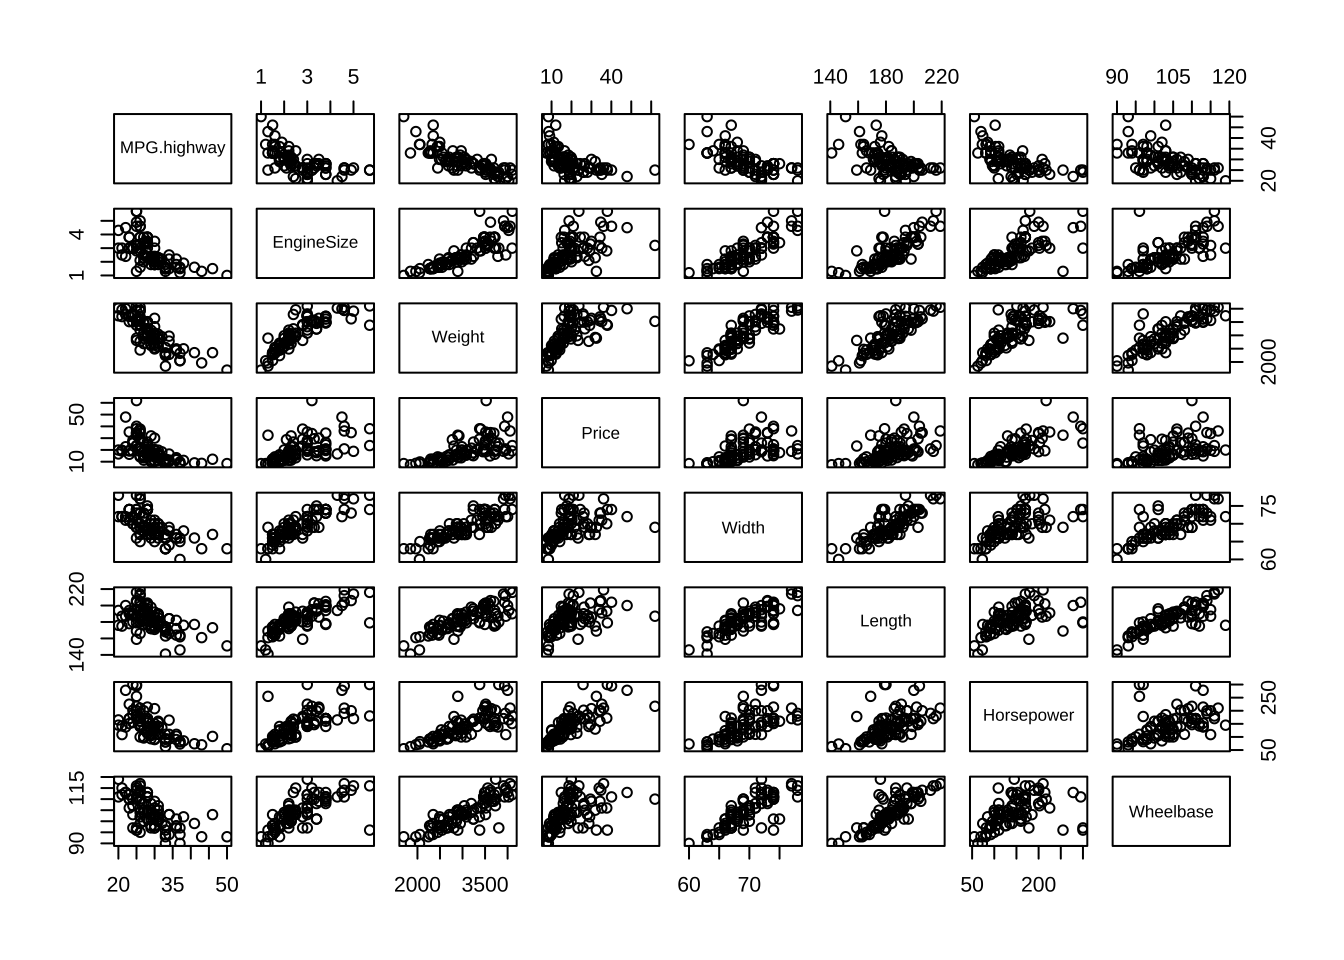
\includegraphics{lmpractice_files/figure-latex/unnamed-chunk-131-1.pdf}

\hypertarget{uxc644uxc804uxbaa8uxd615}{%
\subsection{완전모형}\label{uxc644uxc804uxbaa8uxd615}}

\begin{Shaded}
\begin{Highlighting}[]
\NormalTok{carfit }\OtherTok{\textless{}{-}} \FunctionTok{lm}\NormalTok{(MPG.highway}\SpecialCharTok{\textasciitilde{}}\NormalTok{ . , }\AttributeTok{data=}\NormalTok{dat93)}
\FunctionTok{summary}\NormalTok{(carfit)}
\end{Highlighting}
\end{Shaded}

\begin{verbatim}
## 
## Call:
## lm(formula = MPG.highway ~ ., data = dat93)
## 
## Residuals:
##     Min      1Q  Median      3Q     Max 
## -6.3952 -1.9678 -0.1942  1.4516 10.1313 
## 
## Coefficients:
##              Estimate Std. Error t value Pr(>|t|)    
## (Intercept) 21.119770  12.809426   1.649   0.1029    
## EngineSize   0.483792   0.698257   0.693   0.4903    
## Weight      -0.012833   0.001726  -7.434 7.69e-11 ***
## Price       -0.047157   0.059498  -0.793   0.4302    
## Width        0.079770   0.228192   0.350   0.7275    
## Length       0.058766   0.043322   1.356   0.1785    
## Horsepower   0.013296   0.013443   0.989   0.3254    
## Wheelbase    0.277231   0.118027   2.349   0.0212 *  
## ---
## Signif. codes:  0 '***' 0.001 '**' 0.01 '*' 0.05 '.' 0.1 ' ' 1
## 
## Residual standard error: 2.95 on 85 degrees of freedom
## Multiple R-squared:  0.7172, Adjusted R-squared:  0.694 
## F-statistic:  30.8 on 7 and 85 DF,  p-value: < 2.2e-16
\end{verbatim}

\hypertarget{uxbaa8uxb4e0-uxac00uxb2a5uxd55c-uxd68cuxadc0}{%
\subsection{모든 가능한 회귀}\label{uxbaa8uxb4e0-uxac00uxb2a5uxd55c-uxd68cuxadc0}}

\begin{Shaded}
\begin{Highlighting}[]
\NormalTok{carfit.rgs1 }\OtherTok{\textless{}{-}} \FunctionTok{regsubsets}\NormalTok{(MPG.highway}\SpecialCharTok{\textasciitilde{}}\NormalTok{ . , }\AttributeTok{data=}\NormalTok{dat93, }\AttributeTok{nbest =} \DecValTok{5}\NormalTok{)}
\FunctionTok{summaryf}\NormalTok{(carfit.rgs1)}
\end{Highlighting}
\end{Shaded}

\begin{verbatim}
##          EngineSize Weight Price Width Length Horsepower Wheelbase       rss       rsq     adjr2        cp       bic
## 1  ( 1 )                 *                                          896.6165 0.6571665 0.6533991 14.057585 -90.49226
## 1  ( 2 )                             *                             1542.8773 0.4100599 0.4035771 88.339137 -40.01409
## 1  ( 3 )          *                                                1587.8306 0.3928714 0.3861997 93.506096 -37.34317
## 1  ( 4 )                                               *           1613.0849 0.3832151 0.3764372 96.408840 -35.87565
## 1  ( 5 )                                                         * 1624.8991 0.3786978 0.3718703 97.766767 -35.19700
## 2  ( 1 )                 *                  *                       805.0012 0.6921969 0.6853568  5.527269 -95.98362
## 2  ( 2 )                 *                                       *  805.4566 0.6920227 0.6851788  5.579611 -95.93103
## 2  ( 3 )                 *           *                              843.6064 0.6774356 0.6702675  9.964575 -91.62729
## 2  ( 4 )          *      *                                          865.5483 0.6690459 0.6616913 12.486580 -89.23932
## 2  ( 5 )                 *     *                                    890.7715 0.6594014 0.6518325 15.385756 -86.56791
## 3  ( 1 )                 *                  *                    *  767.5878 0.7065024 0.6966092  3.226956 -95.87697
## 3  ( 2 )          *      *                                       *  772.5928 0.7045887 0.6946310  3.802229 -95.27255
## 3  ( 3 )                 *           *                           *  774.1634 0.7039881 0.6940102  3.982755 -95.08368
## 3  ( 4 )                 *           *      *                       791.2928 0.6974384 0.6872397  5.951620 -93.04836
## 3  ( 5 )                 *                             *         *  793.6299 0.6965448 0.6863160  6.220248 -92.77409
## 4  ( 1 )          *      *                  *                    *  753.0560 0.7120588 0.6989706  3.556655 -93.12192
## 4  ( 2 )                 *           *      *                    *  754.8013 0.7113915 0.6982729  3.757264 -92.90662
## 4  ( 3 )                 *                  *          *         *  759.7929 0.7094829 0.6962776  4.331000 -92.29363
## 4  ( 4 )          *      *           *                           *  762.8251 0.7083235 0.6950655  4.679521 -91.92322
## 4  ( 5 )                 *           *                 *         *  765.6667 0.7072370 0.6939295  5.006135 -91.57743
## 5  ( 1 )                 *           *      *          *         *  748.1512 0.7139342 0.6974936  4.992904 -89.19702
## 5  ( 2 )                 *     *            *          *         *  748.3100 0.7138735 0.6974295  5.011151 -89.17728
## 5  ( 3 )          *      *           *      *                    *  748.4773 0.7138095 0.6973618  5.030385 -89.15649
## 5  ( 4 )          *      *                  *          *         *  750.2487 0.7131322 0.6966456  5.233988 -88.93665
## 5  ( 5 )          *      *     *            *                    *  750.8656 0.7128963 0.6963961  5.304898 -88.86021
## 6  ( 1 )          *      *     *            *          *         *  740.5760 0.7168307 0.6970747  6.122202 -85.61087
## 6  ( 2 )                 *     *     *      *          *         *  743.6893 0.7156403 0.6958012  6.480052 -85.22072
## 6  ( 3 )          *      *           *      *          *         *  744.9782 0.7151475 0.6952740  6.628196 -85.05968
## 6  ( 4 )          *      *     *     *      *                    *  748.0234 0.7139831 0.6940284  6.978214 -84.68030
## 6  ( 5 )          *      *     *     *                 *         *  755.5217 0.7111160 0.6909613  7.840067 -83.75271
## 7  ( 1 )          *      *     *     *      *          *         *  739.5128 0.7172372 0.6939509  8.000000 -81.21187
\end{verbatim}

\begin{Shaded}
\begin{Highlighting}[]
\NormalTok{res1 }\OtherTok{\textless{}{-}} \FunctionTok{ols\_step\_all\_possible}\NormalTok{(carfit)}
\NormalTok{res1}
\end{Highlighting}
\end{Shaded}

\begin{verbatim}
##     Index N                                                Predictors  R-Square Adj. R-Square Mallow's Cp
## 2       1 1                                                    Weight 0.6571665     0.6533991   14.057585
## 4       2 1                                                     Width 0.4100599     0.4035771   88.339137
## 1       3 1                                                EngineSize 0.3928714     0.3861997   93.506096
## 6       4 1                                                Horsepower 0.3832151     0.3764372   96.408840
## 7       5 1                                                 Wheelbase 0.3786978     0.3718703   97.766767
## 3       6 1                                                     Price 0.3143625     0.3068280  117.106304
## 5       7 1                                                    Length 0.2947376     0.2869875  123.005644
## 16      8 2                                             Weight Length 0.6921969     0.6853568    5.527269
## 18      9 2                                          Weight Wheelbase 0.6920227     0.6851788    5.579611
## 15     10 2                                              Weight Width 0.6774356     0.6702675    9.964575
## 8      11 2                                         EngineSize Weight 0.6690459     0.6616913   12.486580
## 14     12 2                                              Weight Price 0.6594014     0.6518325   15.385756
## 17     13 2                                         Weight Horsepower 0.6580588     0.6504601   15.789345
## 28     14 2                                      Horsepower Wheelbase 0.5124413     0.5016067   59.562737
## 19     15 2                                               Price Width 0.5011887     0.4901040   62.945341
## 24     16 2                                          Width Horsepower 0.4829068     0.4714158   68.440980
## 22     17 2                                           Price Wheelbase 0.4637749     0.4518588   74.192130
## 12     18 2                                     EngineSize Horsepower 0.4481507     0.4358874   78.888844
## 9      19 2                                          EngineSize Price 0.4467943     0.4345009   79.296576
## 13     20 2                                      EngineSize Wheelbase 0.4455600     0.4332391   79.667620
## 26     21 2                                         Length Horsepower 0.4417305     0.4293245   80.818789
## 25     22 2                                           Width Wheelbase 0.4378948     0.4254036   81.971816
## 10     23 2                                          EngineSize Width 0.4306826     0.4180311   84.139838
## 23     24 2                                              Width Length 0.4108926     0.3978014   90.088817
## 20     25 2                                              Price Length 0.4053002     0.3920847   91.769933
## 11     26 2                                         EngineSize Length 0.4002766     0.3869495   93.280046
## 21     27 2                                          Price Horsepower 0.3971861     0.3837902   94.209084
## 27     28 2                                          Length Wheelbase 0.3827357     0.3690187   98.552954
## 52     29 3                                   Weight Length Wheelbase 0.7065024     0.6966092    3.226956
## 33     30 3                               EngineSize Weight Wheelbase 0.7045887     0.6946310    3.802229
## 50     31 3                                    Weight Width Wheelbase 0.7039881     0.6940102    3.982755
## 48     32 3                                       Weight Width Length 0.6974384     0.6872397    5.951620
## 53     33 3                               Weight Horsepower Wheelbase 0.6965448     0.6863160    6.220248
## 31     34 3                                  EngineSize Weight Length 0.6950183     0.6847380    6.679132
## 45     35 3                                       Weight Price Length 0.6937780     0.6834559    7.051965
## 51     36 3                                  Weight Length Horsepower 0.6922759     0.6819032    7.503506
## 47     37 3                                    Weight Price Wheelbase 0.6922722     0.6818993    7.504634
## 30     38 3                                   EngineSize Weight Width 0.6794213     0.6686152   11.367681
## 49     39 3                                   Weight Width Horsepower 0.6782765     0.6674319   11.711807
## 44     40 3                                        Weight Price Width 0.6774605     0.6665884   11.957097
## 32     41 3                              EngineSize Weight Horsepower 0.6733325     0.6623213   13.197988
## 29     42 3                                   EngineSize Weight Price 0.6727979     0.6617687   13.358684
## 46     43 3                                   Weight Price Horsepower 0.6594042     0.6479235   17.384909
## 62     44 3                                Width Horsepower Wheelbase 0.5179793     0.5017314   59.897990
## 63     45 3                               Length Horsepower Wheelbase 0.5148833     0.4985310   60.828677
## 59     46 3                                Price Horsepower Wheelbase 0.5141107     0.4977324   61.060911
## 43     47 3                           EngineSize Horsepower Wheelbase 0.5137122     0.4973205   61.180715
## 56     48 3                                     Price Width Wheelbase 0.5099474     0.4934288   62.312418
## 55     49 3                                    Price Width Horsepower 0.5066130     0.4899820   63.314768
## 54     50 3                                        Price Width Length 0.5036344     0.4869030   64.210137
## 34     51 3                                    EngineSize Price Width 0.5012349     0.4844226   64.931444
## 37     52 3                                EngineSize Price Wheelbase 0.4884132     0.4711687   68.785739
## 39     53 3                               EngineSize Width Horsepower 0.4834512     0.4660395   70.277316
## 60     54 3                                   Width Length Horsepower 0.4831570     0.4657353   70.365777
## 58     55 3                                    Price Length Wheelbase 0.4638667     0.4457948   76.164543
## 36     56 3                               EngineSize Price Horsepower 0.4593761     0.4411528   77.514439
## 41     57 3                              EngineSize Length Horsepower 0.4576417     0.4393599   78.035815
## 40     58 3                                EngineSize Width Wheelbase 0.4537493     0.4353363   79.205884
## 35     59 3                                   EngineSize Price Length 0.4515414     0.4330540   79.869587
## 42     60 3                               EngineSize Length Wheelbase 0.4493877     0.4308278   80.516993
## 57     61 3                                   Price Length Horsepower 0.4491768     0.4306097   80.580389
## 61     62 3                                    Width Length Wheelbase 0.4412041     0.4223683   82.977030
## 38     63 3                                   EngineSize Width Length 0.4307121     0.4115226   86.130983
## 72     64 4                        EngineSize Weight Length Wheelbase 0.7120588     0.6989706    3.556655
## 91     65 4                             Weight Width Length Wheelbase 0.7113915     0.6982729    3.757264
## 93     66 4                        Weight Length Horsepower Wheelbase 0.7094829     0.6962776    4.331000
## 70     67 4                         EngineSize Weight Width Wheelbase 0.7083235     0.6950655    4.679521
## 92     68 4                         Weight Width Horsepower Wheelbase 0.7072370     0.6939295    5.006135
## 88     69 4                             Weight Price Length Wheelbase 0.7068981     0.6935753    5.107983
## 73     70 4                    EngineSize Weight Horsepower Wheelbase 0.7056067     0.6922252    5.496208
## 67     71 4                         EngineSize Weight Price Wheelbase 0.7054766     0.6920891    5.535316
## 86     72 4                              Weight Price Width Wheelbase 0.7042113     0.6907663    5.915667
## 89     73 4                         Weight Price Horsepower Wheelbase 0.7015381     0.6879717    6.719233
## 68     74 4                            EngineSize Weight Width Length 0.6980586     0.6843340    7.765190
## 84     75 4                                 Weight Price Width Length 0.6977722     0.6840346    7.851291
## 90     76 4                            Weight Width Length Horsepower 0.6975840     0.6838378    7.907857
## 65     77 4                            EngineSize Weight Price Length 0.6973130     0.6835545    7.989316
## 71     78 4                       EngineSize Weight Length Horsepower 0.6958959     0.6820730    8.415308
## 87     79 4                            Weight Price Length Horsepower 0.6941365     0.6802336    8.944197
## 69     80 4                        EngineSize Weight Width Horsepower 0.6816709     0.6672014   12.691426
## 64     81 4                             EngineSize Weight Price Width 0.6798490     0.6652967   13.239103
## 85     82 4                             Weight Price Width Horsepower 0.6785699     0.6639594   13.623605
## 66     83 4                        EngineSize Weight Price Horsepower 0.6740921     0.6592781   14.969666
## 98     84 4                         Width Length Horsepower Wheelbase 0.5251823     0.5035997   59.732737
## 96     85 4                          Price Width Horsepower Wheelbase 0.5241486     0.5025189   60.043486
## 95     86 4                              Price Width Length Wheelbase 0.5201414     0.4983296   61.248067
## 83     87 4                    EngineSize Length Horsepower Wheelbase 0.5181794     0.4962785   61.837835
## 82     88 4                     EngineSize Width Horsepower Wheelbase 0.5180310     0.4961233   61.882452
## 97     89 4                         Price Length Horsepower Wheelbase 0.5163650     0.4943816   62.383258
## 79     90 4                     EngineSize Price Horsepower Wheelbase 0.5157712     0.4937608   62.561774
## 76     91 4                          EngineSize Price Width Wheelbase 0.5100005     0.4877278   64.296462
## 94     92 4                             Price Width Length Horsepower 0.5078459     0.4854753   64.944142
## 75     93 4                         EngineSize Price Width Horsepower 0.5066821     0.4842586   65.293996
## 74     94 4                             EngineSize Price Width Length 0.5038288     0.4812756   66.151710
## 78     95 4                         EngineSize Price Length Wheelbase 0.4924386     0.4693677   69.575658
## 80     96 4                        EngineSize Width Length Horsepower 0.4835609     0.4600864   72.244351
## 77     97 4                        EngineSize Price Length Horsepower 0.4663693     0.4421134   77.412237
## 81     98 4                         EngineSize Width Length Wheelbase 0.4611666     0.4366742   78.976188
## 118    99 5                  Weight Width Length Horsepower Wheelbase 0.7139342     0.6974936    4.992904
## 117   100 5                  Weight Price Length Horsepower Wheelbase 0.7138735     0.6974295    5.011151
## 106   101 5                  EngineSize Weight Width Length Wheelbase 0.7138095     0.6973618    5.030385
## 108   102 5             EngineSize Weight Length Horsepower Wheelbase 0.7131322     0.6966456    5.233988
## 103   103 5                  EngineSize Weight Price Length Wheelbase 0.7128963     0.6963961    5.304898
## 115   104 5                       Weight Price Width Length Wheelbase 0.7113951     0.6948086    5.756187
## 107   105 5              EngineSize Weight Width Horsepower Wheelbase 0.7097227     0.6930401    6.258900
## 104   106 5              EngineSize Weight Price Horsepower Wheelbase 0.7093581     0.6926546    6.368497
## 101   107 5                   EngineSize Weight Price Width Wheelbase 0.7083618     0.6916010    6.667986
## 116   108 5                   Weight Price Width Horsepower Wheelbase 0.7081360     0.6913622    6.735874
## 99    109 5                      EngineSize Weight Price Width Length 0.6988219     0.6815128    9.535752
## 105   110 5                 EngineSize Weight Width Length Horsepower 0.6985844     0.6812617    9.607135
## 114   111 5                      Weight Price Width Length Horsepower 0.6977723     0.6804029    9.851269
## 102   112 5                 EngineSize Weight Price Length Horsepower 0.6973147     0.6799190    9.988818
## 100   113 5                  EngineSize Weight Price Width Horsepower 0.6817449     0.6634544   14.669181
## 119   114 5                   Price Width Length Horsepower Wheelbase 0.5333826     0.5065655   59.267687
## 113   115 5              EngineSize Width Length Horsepower Wheelbase 0.5252650     0.4979813   61.707890
## 111   116 5               EngineSize Price Width Horsepower Wheelbase 0.5245145     0.4971878   61.933476
## 110   117 5                   EngineSize Price Width Length Wheelbase 0.5207064     0.4931608   63.078211
## 112   118 5              EngineSize Price Length Horsepower Wheelbase 0.5201984     0.4926236   63.230914
## 109   119 5                  EngineSize Price Width Length Horsepower 0.5078486     0.4795640   66.943339
## 123   120 6       EngineSize Weight Price Length Horsepower Wheelbase 0.7168307     0.6970747    6.122202
## 126   121 6            Weight Price Width Length Horsepower Wheelbase 0.7156403     0.6958012    6.480052
## 124   122 6       EngineSize Weight Width Length Horsepower Wheelbase 0.7151475     0.6952740    6.628196
## 121   123 6            EngineSize Weight Price Width Length Wheelbase 0.7139831     0.6940284    6.978214
## 122   124 6        EngineSize Weight Price Width Horsepower Wheelbase 0.7111160     0.6909613    7.840067
## 120   125 6           EngineSize Weight Price Width Length Horsepower 0.6988835     0.6778753   11.517234
## 125   126 6        EngineSize Price Width Length Horsepower Wheelbase 0.5333888     0.5008345   61.265830
## 127   127 7 EngineSize Weight Price Width Length Horsepower Wheelbase 0.7172372     0.6939509    8.000000
\end{verbatim}

\begin{Shaded}
\begin{Highlighting}[]
\FunctionTok{plot}\NormalTok{(res1)}
\end{Highlighting}
\end{Shaded}

\includegraphics{lmpractice_files/figure-latex/unnamed-chunk-134-1.pdf} \includegraphics{lmpractice_files/figure-latex/unnamed-chunk-134-2.pdf}

\hypertarget{c_p}{%
\subsection{C\_p}\label{c_p}}

\begin{Shaded}
\begin{Highlighting}[]
\FunctionTok{subsets}\NormalTok{(carfit.rgs1, }\AttributeTok{statistic=}\StringTok{"cp"}\NormalTok{, }\AttributeTok{legend =}\NormalTok{ F, }\AttributeTok{min.size =} \DecValTok{1}\NormalTok{, }\AttributeTok{main =} \StringTok{"Mallow Cp"}\NormalTok{)}
\end{Highlighting}
\end{Shaded}

\begin{verbatim}
##            Abbreviation
## EngineSize            E
## Weight               Wg
## Price                 P
## Width                Wd
## Length                L
## Horsepower            H
## Wheelbase            Wh
\end{verbatim}

\begin{Shaded}
\begin{Highlighting}[]
\FunctionTok{abline}\NormalTok{(}\AttributeTok{a =} \DecValTok{1}\NormalTok{, }\AttributeTok{b =} \DecValTok{1}\NormalTok{, }\AttributeTok{lty =} \DecValTok{2}\NormalTok{)}
\end{Highlighting}
\end{Shaded}

\includegraphics{lmpractice_files/figure-latex/unnamed-chunk-135-1.pdf}

\hypertarget{uxc804uxc9c4uxc120uxd0dduxbc95-1}{%
\subsection{전진선택법}\label{uxc804uxc9c4uxc120uxd0dduxbc95-1}}

\begin{Shaded}
\begin{Highlighting}[]
\NormalTok{model0 }\OtherTok{\textless{}{-}} \FunctionTok{lm}\NormalTok{(MPG.highway}\SpecialCharTok{\textasciitilde{}}\DecValTok{1}\NormalTok{, }\AttributeTok{data=}\NormalTok{dat93)}
\FunctionTok{step}\NormalTok{(model0,  }\AttributeTok{scope=}\SpecialCharTok{\textasciitilde{}}\NormalTok{EngineSize}\SpecialCharTok{+}\NormalTok{ Weight}\SpecialCharTok{+}\NormalTok{ Price}\SpecialCharTok{+}\NormalTok{ Width}\SpecialCharTok{+}\NormalTok{ Length}\SpecialCharTok{+}\NormalTok{ Horsepower}\SpecialCharTok{+}\NormalTok{ Wheelbase, }\AttributeTok{direction=}\StringTok{"forward"}\NormalTok{)}
\end{Highlighting}
\end{Shaded}

\begin{verbatim}
## Start:  AIC=312.3
## MPG.highway ~ 1
## 
##              Df Sum of Sq     RSS    AIC
## + Weight      1   1718.70  896.62 214.74
## + Width       1   1072.43 1542.88 265.22
## + EngineSize  1   1027.48 1587.83 267.89
## + Horsepower  1   1002.23 1613.08 269.36
## + Wheelbase   1    990.41 1624.90 270.04
## + Price       1    822.16 1793.16 279.20
## + Length      1    770.83 1844.48 281.82
## <none>                    2615.31 312.30
## 
## Step:  AIC=214.74
## MPG.highway ~ Weight
## 
##              Df Sum of Sq    RSS    AIC
## + Length      1    91.615 805.00 206.72
## + Wheelbase   1    91.160 805.46 206.77
## + Width       1    53.010 843.61 211.07
## + EngineSize  1    31.068 865.55 213.46
## <none>                    896.62 214.74
## + Price       1     5.845 890.77 216.13
## + Horsepower  1     2.334 894.28 216.50
## 
## Step:  AIC=206.72
## MPG.highway ~ Weight + Length
## 
##              Df Sum of Sq    RSS    AIC
## + Wheelbase   1    37.413 767.59 204.29
## <none>                    805.00 206.72
## + Width       1    13.708 791.29 207.12
## + EngineSize  1     7.379 797.62 207.86
## + Price       1     4.135 800.87 208.24
## + Horsepower  1     0.207 804.79 208.69
## 
## Step:  AIC=204.29
## MPG.highway ~ Weight + Length + Wheelbase
## 
##              Df Sum of Sq    RSS    AIC
## <none>                    767.59 204.29
## + EngineSize  1   14.5319 753.06 204.51
## + Width       1   12.7865 754.80 204.73
## + Horsepower  1    7.7950 759.79 205.34
## + Price       1    1.0351 766.55 206.16
\end{verbatim}

\begin{verbatim}
## 
## Call:
## lm(formula = MPG.highway ~ Weight + Length + Wheelbase, data = dat93)
## 
## Coefficients:
## (Intercept)       Weight       Length    Wheelbase  
##    26.31687     -0.01107      0.08170      0.21005
\end{verbatim}

\hypertarget{uxd6c4uxbc29uxc81cuxac70-1}{%
\subsection{후방제거}\label{uxd6c4uxbc29uxc81cuxac70-1}}

\begin{Shaded}
\begin{Highlighting}[]
\FunctionTok{step}\NormalTok{(carfit, }\AttributeTok{direction=}\StringTok{"backward"}\NormalTok{)}
\end{Highlighting}
\end{Shaded}

\begin{verbatim}
## Start:  AIC=208.83
## MPG.highway ~ EngineSize + Weight + Price + Width + Length + 
##     Horsepower + Wheelbase
## 
##              Df Sum of Sq     RSS    AIC
## - Width       1      1.06  740.58 206.96
## - EngineSize  1      4.18  743.69 207.35
## - Price       1      5.47  744.98 207.51
## - Horsepower  1      8.51  748.02 207.89
## - Length      1     16.01  755.52 208.82
## <none>                     739.51 208.82
## - Wheelbase   1     48.00  787.51 212.67
## - Weight      1    480.82 1220.33 253.41
## 
## Step:  AIC=206.96
## MPG.highway ~ EngineSize + Weight + Price + Length + Horsepower + 
##     Wheelbase
## 
##              Df Sum of Sq     RSS    AIC
## - EngineSize  1      7.73  748.31 205.93
## - Price       1      9.67  750.25 206.17
## - Horsepower  1     10.29  750.87 206.24
## <none>                     740.58 206.96
## - Length      1     19.54  760.12 207.38
## - Wheelbase   1     51.04  791.62 211.16
## - Weight      1    514.25 1254.83 254.00
## 
## Step:  AIC=205.93
## MPG.highway ~ Weight + Price + Length + Horsepower + Wheelbase
## 
##              Df Sum of Sq     RSS    AIC
## - Price       1     11.48  759.79 205.34
## <none>                     748.31 205.93
## - Horsepower  1     18.24  766.55 206.16
## - Length      1     32.26  780.57 207.85
## - Wheelbase   1     51.62  799.93 210.13
## - Weight      1    516.55 1264.86 252.74
## 
## Step:  AIC=205.34
## MPG.highway ~ Weight + Length + Horsepower + Wheelbase
## 
##              Df Sum of Sq     RSS    AIC
## - Horsepower  1      7.79  767.59 204.29
## <none>                     759.79 205.34
## - Length      1     33.84  793.63 207.39
## - Wheelbase   1     45.00  804.79 208.69
## - Weight      1    508.94 1268.73 251.03
## 
## Step:  AIC=204.29
## MPG.highway ~ Weight + Length + Wheelbase
## 
##             Df Sum of Sq     RSS    AIC
## <none>                    767.59 204.29
## - Wheelbase  1     37.41  805.00 206.72
## - Length     1     37.87  805.46 206.77
## - Weight     1    846.75 1614.34 271.43
\end{verbatim}

\begin{verbatim}
## 
## Call:
## lm(formula = MPG.highway ~ Weight + Length + Wheelbase, data = dat93)
## 
## Coefficients:
## (Intercept)       Weight       Length    Wheelbase  
##    26.31687     -0.01107      0.08170      0.21005
\end{verbatim}

\hypertarget{uxb2e8uxacc4uxbcc4-uxc120uxd0dd-1}{%
\subsection{단계별 선택}\label{uxb2e8uxacc4uxbcc4-uxc120uxd0dd-1}}

\begin{Shaded}
\begin{Highlighting}[]
\NormalTok{model0 }\OtherTok{\textless{}{-}} \FunctionTok{lm}\NormalTok{(MPG.highway}\SpecialCharTok{\textasciitilde{}}\DecValTok{1}\NormalTok{, }\AttributeTok{data=}\NormalTok{dat93)}
\FunctionTok{step}\NormalTok{(model0,  }\AttributeTok{scope=}\SpecialCharTok{\textasciitilde{}}\NormalTok{EngineSize}\SpecialCharTok{+}\NormalTok{ Weight}\SpecialCharTok{+}\NormalTok{ Price}\SpecialCharTok{+}\NormalTok{ Width}\SpecialCharTok{+}\NormalTok{ Length}\SpecialCharTok{+}\NormalTok{ Horsepower}\SpecialCharTok{+}\NormalTok{ Wheelbase, }\AttributeTok{direction=}\StringTok{"both"}\NormalTok{)}
\end{Highlighting}
\end{Shaded}

\begin{verbatim}
## Start:  AIC=312.3
## MPG.highway ~ 1
## 
##              Df Sum of Sq     RSS    AIC
## + Weight      1   1718.70  896.62 214.74
## + Width       1   1072.43 1542.88 265.22
## + EngineSize  1   1027.48 1587.83 267.89
## + Horsepower  1   1002.23 1613.08 269.36
## + Wheelbase   1    990.41 1624.90 270.04
## + Price       1    822.16 1793.16 279.20
## + Length      1    770.83 1844.48 281.82
## <none>                    2615.31 312.30
## 
## Step:  AIC=214.74
## MPG.highway ~ Weight
## 
##              Df Sum of Sq     RSS    AIC
## + Length      1     91.62  805.00 206.72
## + Wheelbase   1     91.16  805.46 206.77
## + Width       1     53.01  843.61 211.07
## + EngineSize  1     31.07  865.55 213.46
## <none>                     896.62 214.74
## + Price       1      5.85  890.77 216.13
## + Horsepower  1      2.33  894.28 216.50
## - Weight      1   1718.70 2615.31 312.30
## 
## Step:  AIC=206.72
## MPG.highway ~ Weight + Length
## 
##              Df Sum of Sq     RSS    AIC
## + Wheelbase   1     37.41  767.59 204.29
## <none>                     805.00 206.72
## + Width       1     13.71  791.29 207.12
## + EngineSize  1      7.38  797.62 207.86
## + Price       1      4.14  800.87 208.24
## + Horsepower  1      0.21  804.79 208.69
## - Length      1     91.62  896.62 214.74
## - Weight      1   1039.48 1844.48 281.82
## 
## Step:  AIC=204.29
## MPG.highway ~ Weight + Length + Wheelbase
## 
##              Df Sum of Sq     RSS    AIC
## <none>                     767.59 204.29
## + EngineSize  1     14.53  753.06 204.51
## + Width       1     12.79  754.80 204.73
## + Horsepower  1      7.79  759.79 205.34
## + Price       1      1.04  766.55 206.16
## - Wheelbase   1     37.41  805.00 206.72
## - Length      1     37.87  805.46 206.77
## - Weight      1    846.75 1614.34 271.43
\end{verbatim}

\begin{verbatim}
## 
## Call:
## lm(formula = MPG.highway ~ Weight + Length + Wheelbase, data = dat93)
## 
## Coefficients:
## (Intercept)       Weight       Length    Wheelbase  
##    26.31687     -0.01107      0.08170      0.21005
\end{verbatim}

\begin{Shaded}
\begin{Highlighting}[]
\FunctionTok{ols\_step\_forward\_aic}\NormalTok{(carfit, }\AttributeTok{details =} \ConstantTok{TRUE}\NormalTok{)}
\end{Highlighting}
\end{Shaded}

\begin{verbatim}
## Forward Selection Method 
## ------------------------
## 
## Candidate Terms: 
## 
## 1 . EngineSize 
## 2 . Weight 
## 3 . Price 
## 4 . Width 
## 5 . Length 
## 6 . Horsepower 
## 7 . Wheelbase 
## 
##  Step 0: AIC = 578.2207 
##  MPG.highway ~ 1 
## 
## -------------------------------------------------------------------------
## Variable      DF      AIC       Sum Sq       RSS       R-Sq     Adj. R-Sq 
## -------------------------------------------------------------------------
## Weight         1    480.663    1718.695     896.617    0.657        0.653 
## Width          1    531.141    1072.435    1542.877    0.410        0.404 
## EngineSize     1    533.812    1027.481    1587.831    0.393        0.386 
## Horsepower     1    535.280    1002.227    1613.085    0.383        0.376 
## Wheelbase      1    535.959     990.413    1624.899    0.379        0.372 
## Price          1    545.122     822.156    1793.156    0.314        0.307 
## Length         1    547.746     770.831    1844.481    0.295        0.287 
## -------------------------------------------------------------------------
## 
## 
## - Weight 
## 
## 
##  Step 1 : AIC = 480.6632 
##  MPG.highway ~ Weight 
## 
## ----------------------------------------------------------------------
## Variable      DF      AIC      Sum Sq      RSS      R-Sq     Adj. R-Sq 
## ----------------------------------------------------------------------
## Length         1    472.639    91.615    805.001    0.692        0.685 
## Wheelbase      1    472.692    91.160    805.457    0.692        0.685 
## Width          1    476.996    53.010    843.606    0.677        0.670 
## EngineSize     1    479.384    31.068    865.548    0.669        0.662 
## Price          1    482.055     5.845    890.772    0.659        0.652 
## Horsepower     1    482.421     2.334    894.283    0.658        0.650 
## ----------------------------------------------------------------------
## 
## - Length 
## 
## 
##  Step 2 : AIC = 472.6393 
##  MPG.highway ~ Weight + Length 
## 
## ----------------------------------------------------------------------
## Variable      DF      AIC      Sum Sq      RSS      R-Sq     Adj. R-Sq 
## ----------------------------------------------------------------------
## Wheelbase      1    470.213    37.413    767.588    0.707        0.697 
## Width          1    473.042    13.708    791.293    0.697        0.687 
## EngineSize     1    473.783     7.379    797.622    0.695        0.685 
## Price          1    474.160     4.135    800.866    0.694        0.683 
## Horsepower     1    474.615     0.207    804.794    0.692        0.682 
## ----------------------------------------------------------------------
## 
## - Wheelbase 
## 
## 
##  Step 3 : AIC = 470.2133 
##  MPG.highway ~ Weight + Length + Wheelbase 
## 
## ----------------------------------------------------------------------
## Variable      DF      AIC      Sum Sq      RSS      R-Sq     Adj. R-Sq 
## ----------------------------------------------------------------------
## EngineSize     1    470.436    14.532    753.056    0.712        0.699 
## Width          1    470.651    12.787    754.801    0.711        0.698 
## Horsepower     1    471.264     7.795    759.793    0.709        0.696 
## Price          1    472.088     1.035    766.553    0.707        0.694 
## ----------------------------------------------------------------------
## 
## 
## No more variables to be added.
## 
## Variables Entered: 
## 
## - Weight 
## - Length 
## - Wheelbase 
## 
## 
## Final Model Output 
## ------------------
## 
##                         Model Summary                          
## --------------------------------------------------------------
## R                       0.841       RMSE                2.937 
## R-Squared               0.707       Coef. Var          10.097 
## Adj. R-Squared          0.697       MSE                 8.625 
## Pred R-Squared          0.665       MAE                 2.139 
## --------------------------------------------------------------
##  RMSE: Root Mean Square Error 
##  MSE: Mean Square Error 
##  MAE: Mean Absolute Error 
## 
##                                ANOVA                                 
## --------------------------------------------------------------------
##                 Sum of                                              
##                Squares        DF    Mean Square      F         Sig. 
## --------------------------------------------------------------------
## Regression    1847.724         3        615.908    71.413    0.0000 
## Residual       767.588        89          8.625                     
## Total         2615.312        92                                    
## --------------------------------------------------------------------
## 
##                                   Parameter Estimates                                    
## ----------------------------------------------------------------------------------------
##       model      Beta    Std. Error    Std. Beta      t        Sig      lower     upper 
## ----------------------------------------------------------------------------------------
## (Intercept)    26.317         7.088                  3.713    0.000    12.233    40.401 
##      Weight    -0.011         0.001       -1.225    -9.909    0.000    -0.013    -0.009 
##      Length     0.082         0.039        0.224     2.095    0.039     0.004     0.159 
##   Wheelbase     0.210         0.101        0.269     2.083    0.040     0.010     0.410 
## ----------------------------------------------------------------------------------------
\end{verbatim}

\begin{verbatim}
## 
##                          Selection Summary                          
## -------------------------------------------------------------------
## Variable       AIC       Sum Sq       RSS       R-Sq      Adj. R-Sq 
## -------------------------------------------------------------------
## Weight       480.663    1718.695    896.617    0.65717      0.65340 
## Length       472.639    1810.311    805.001    0.69220      0.68536 
## Wheelbase    470.213    1847.724    767.588    0.70650      0.69661 
## -------------------------------------------------------------------
\end{verbatim}

\begin{Shaded}
\begin{Highlighting}[]
\FunctionTok{ols\_step\_forward\_p}\NormalTok{(carfit, }\AttributeTok{details =} \ConstantTok{TRUE}\NormalTok{)}
\end{Highlighting}
\end{Shaded}

\begin{verbatim}
## Forward Selection Method    
## ---------------------------
## 
## Candidate Terms: 
## 
## 1. EngineSize 
## 2. Weight 
## 3. Price 
## 4. Width 
## 5. Length 
## 6. Horsepower 
## 7. Wheelbase 
## 
## We are selecting variables based on p value...
## 
## 
## Forward Selection: Step 1 
## 
## - Weight 
## 
##                         Model Summary                          
## --------------------------------------------------------------
## R                       0.811       RMSE                3.139 
## R-Squared               0.657       Coef. Var          10.792 
## Adj. R-Squared          0.653       MSE                 9.853 
## Pred R-Squared          0.635       MAE                 2.290 
## --------------------------------------------------------------
##  RMSE: Root Mean Square Error 
##  MSE: Mean Square Error 
##  MAE: Mean Absolute Error 
## 
##                                 ANOVA                                 
## ---------------------------------------------------------------------
##                 Sum of                                               
##                Squares        DF    Mean Square       F         Sig. 
## ---------------------------------------------------------------------
## Regression    1718.695         1       1718.695    174.435    0.0000 
## Residual       896.617        91          9.853                      
## Total         2615.312        92                                     
## ---------------------------------------------------------------------
## 
##                                    Parameter Estimates                                    
## -----------------------------------------------------------------------------------------
##       model      Beta    Std. Error    Std. Beta       t        Sig      lower     upper 
## -----------------------------------------------------------------------------------------
## (Intercept)    51.601         1.736                  29.732    0.000    48.154    55.049 
##      Weight    -0.007         0.001       -0.811    -13.207    0.000    -0.008    -0.006 
## -----------------------------------------------------------------------------------------
## 
## 
## 
## Forward Selection: Step 2 
## 
## - Length 
## 
##                         Model Summary                          
## --------------------------------------------------------------
## R                       0.832       RMSE                2.991 
## R-Squared               0.692       Coef. Var          10.282 
## Adj. R-Squared          0.685       MSE                 8.944 
## Pred R-Squared          0.667       MAE                 2.122 
## --------------------------------------------------------------
##  RMSE: Root Mean Square Error 
##  MSE: Mean Square Error 
##  MAE: Mean Absolute Error 
## 
##                                 ANOVA                                 
## ---------------------------------------------------------------------
##                 Sum of                                               
##                Squares        DF    Mean Square       F         Sig. 
## ---------------------------------------------------------------------
## Regression    1810.311         2        905.155    101.197    0.0000 
## Residual       805.001        90          8.944                      
## Total         2615.312        92                                     
## ---------------------------------------------------------------------
## 
##                                    Parameter Estimates                                    
## -----------------------------------------------------------------------------------------
##       model      Beta    Std. Error    Std. Beta       t        Sig      lower     upper 
## -----------------------------------------------------------------------------------------
## (Intercept)    37.522         4.700                   7.984    0.000    28.185    46.859 
##      Weight    -0.010         0.001       -1.066    -10.780    0.000    -0.011    -0.008 
##      Length     0.116         0.036        0.316      3.200    0.002     0.044     0.187 
## -----------------------------------------------------------------------------------------
## 
## 
## 
## Forward Selection: Step 3 
## 
## - Wheelbase 
## 
##                         Model Summary                          
## --------------------------------------------------------------
## R                       0.841       RMSE                2.937 
## R-Squared               0.707       Coef. Var          10.097 
## Adj. R-Squared          0.697       MSE                 8.625 
## Pred R-Squared          0.665       MAE                 2.139 
## --------------------------------------------------------------
##  RMSE: Root Mean Square Error 
##  MSE: Mean Square Error 
##  MAE: Mean Absolute Error 
## 
##                                ANOVA                                 
## --------------------------------------------------------------------
##                 Sum of                                              
##                Squares        DF    Mean Square      F         Sig. 
## --------------------------------------------------------------------
## Regression    1847.724         3        615.908    71.413    0.0000 
## Residual       767.588        89          8.625                     
## Total         2615.312        92                                    
## --------------------------------------------------------------------
## 
##                                   Parameter Estimates                                    
## ----------------------------------------------------------------------------------------
##       model      Beta    Std. Error    Std. Beta      t        Sig      lower     upper 
## ----------------------------------------------------------------------------------------
## (Intercept)    26.317         7.088                  3.713    0.000    12.233    40.401 
##      Weight    -0.011         0.001       -1.225    -9.909    0.000    -0.013    -0.009 
##      Length     0.082         0.039        0.224     2.095    0.039     0.004     0.159 
##   Wheelbase     0.210         0.101        0.269     2.083    0.040     0.010     0.410 
## ----------------------------------------------------------------------------------------
## 
## 
## 
## Forward Selection: Step 4 
## 
## - EngineSize 
## 
##                         Model Summary                          
## --------------------------------------------------------------
## R                       0.844       RMSE                2.925 
## R-Squared               0.712       Coef. Var          10.057 
## Adj. R-Squared          0.699       MSE                 8.557 
## Pred R-Squared          0.664       MAE                 2.081 
## --------------------------------------------------------------
##  RMSE: Root Mean Square Error 
##  MSE: Mean Square Error 
##  MAE: Mean Absolute Error 
## 
##                                ANOVA                                 
## --------------------------------------------------------------------
##                 Sum of                                              
##                Squares        DF    Mean Square      F         Sig. 
## --------------------------------------------------------------------
## Regression    1862.256         4        465.564    54.404    0.0000 
## Residual       753.056        88          8.557                     
## Total         2615.312        92                                    
## --------------------------------------------------------------------
## 
##                                   Parameter Estimates                                    
## ----------------------------------------------------------------------------------------
##       model      Beta    Std. Error    Std. Beta      t        Sig      lower     upper 
## ----------------------------------------------------------------------------------------
## (Intercept)    28.439         7.246                  3.925    0.000    14.040    42.839 
##      Weight    -0.012         0.001       -1.334    -8.960    0.000    -0.015    -0.009 
##      Length     0.063         0.041        0.172     1.511    0.134    -0.020     0.145 
##   Wheelbase     0.233         0.102        0.298     2.282    0.025     0.030     0.435 
##  EngineSize     0.766         0.587        0.149     1.303    0.196    -0.402     1.933 
## ----------------------------------------------------------------------------------------
## 
## 
## 
## No more variables to be added.
## 
## Variables Entered: 
## 
## + Weight 
## + Length 
## + Wheelbase 
## + EngineSize 
## 
## 
## Final Model Output 
## ------------------
## 
##                         Model Summary                          
## --------------------------------------------------------------
## R                       0.844       RMSE                2.925 
## R-Squared               0.712       Coef. Var          10.057 
## Adj. R-Squared          0.699       MSE                 8.557 
## Pred R-Squared          0.664       MAE                 2.081 
## --------------------------------------------------------------
##  RMSE: Root Mean Square Error 
##  MSE: Mean Square Error 
##  MAE: Mean Absolute Error 
## 
##                                ANOVA                                 
## --------------------------------------------------------------------
##                 Sum of                                              
##                Squares        DF    Mean Square      F         Sig. 
## --------------------------------------------------------------------
## Regression    1862.256         4        465.564    54.404    0.0000 
## Residual       753.056        88          8.557                     
## Total         2615.312        92                                    
## --------------------------------------------------------------------
## 
##                                   Parameter Estimates                                    
## ----------------------------------------------------------------------------------------
##       model      Beta    Std. Error    Std. Beta      t        Sig      lower     upper 
## ----------------------------------------------------------------------------------------
## (Intercept)    28.439         7.246                  3.925    0.000    14.040    42.839 
##      Weight    -0.012         0.001       -1.334    -8.960    0.000    -0.015    -0.009 
##      Length     0.063         0.041        0.172     1.511    0.134    -0.020     0.145 
##   Wheelbase     0.233         0.102        0.298     2.282    0.025     0.030     0.435 
##  EngineSize     0.766         0.587        0.149     1.303    0.196    -0.402     1.933 
## ----------------------------------------------------------------------------------------
\end{verbatim}

\begin{verbatim}
## 
##                              Selection Summary                              
## ---------------------------------------------------------------------------
##         Variable                    Adj.                                       
## Step     Entered      R-Square    R-Square     C(p)        AIC        RMSE     
## ---------------------------------------------------------------------------
##    1    Weight          0.6572      0.6534    14.0576    480.6632    3.1389    
##    2    Length          0.6922      0.6854     5.5273    472.6393    2.9907    
##    3    Wheelbase       0.7065      0.6966     3.2270    470.2133    2.9368    
##    4    EngineSize      0.7121      0.6990     3.5567    470.4358    2.9253    
## ---------------------------------------------------------------------------
\end{verbatim}

  \bibliography{book.bib,packages.bib}

\end{document}
